%-------------------------------------------------------------------------------

% This file is part of Code_Saturne, a general-purpose CFD tool.
%
% Copyright (C) 1998-2020 EDF S.A.
%
% This program is free software; you can redistribute it and/or modify it under
% the terms of the GNU General Public License as published by the Free Software
% Foundation; either version 2 of the License, or (at your option) any later
% version.
%
% This program is distributed in the hope that it will be useful, but WITHOUT
% ANY WARRANTY; without even the implied warranty of MERCHANTABILITY or FITNESS
% FOR A PARTICULAR PURPOSE.  See the GNU General Public License for more
% details.
%
% You should have received a copy of the GNU General Public License along with
% this program; if not, write to the Free Software Foundation, Inc., 51 Franklin
% Street, Fifth Floor, Boston, MA 02110-1301, USA.

%-------------------------------------------------------------------------------

%%%%%%%%%%%%%%%%%%%%%%%%%%%%%%%%%%%%%%%%%%%%%%%%%%%%%%%%%%%%%%%%%%%%%%
% csdoc class wich is done for reports
\documentclass[a4paper,10pt,twoside]{csshortdoc}
% MACROS SUPPLEMENTAIRES
\usepackage{csmacros}
%
%%%%%%%%%%%%%%%%%%%%%%%%%%%%%%%%%%%%%%%%%%%%%%%%%%%%%%%%%%%%%%%%%%%%%%

%
%%%%%%%%%%%%%%%%%%%%%%%%%%%%%%%%%%%%%%%%%%%%%%%%%%%%%%%%%%%%%%%%%%%%%%
% PACKAGES ET COMMANDES POUR LE DOCUMENTS PDF ET LES HYPERLIENS
\hypersetup{%
  pdftitle = {CodeSaturne practical user's guide},
  pdfauthor = {MFEE},
  pdfpagemode = UseOutlines
}
\pdfinfo{/CreationDate (D:20030429000000-01 00 )}
%
% To have thumbnails upon opening the document under ACROREAD
% pdfpagemode = UseThumbs
%
%%%%%%%%%%%%%%%%%%%%%%%%%%%%%%%%%%%%%%%%%%%%%%%%%%%%%%%%%%%%%%%%%%%%%%
% REALISATION D'UN INDEX
\usepackage{makeidx}
\makeindex
%
%%%%%%%%%%%%%%%%%%%%%%%%%%%%%%%%%%%%%%%%%%%%%%%%%%%%%%%%%%%%%%%%%%%%%%
% PACKAGES ALLTT D'ENVIRONNEMENT VERBATIM AMELIORE
\usepackage{alltt}
%
%%%%%%%%%%%%%%%%%%%%%%%%%%%%%%%%%%%%%%%%%%%%%%%%%%%%%%%%%%%%%%%%%%%%%%
% INFO POUR PAGES DE GARDES
\titreCS{\CS version~\verscs practical user's guide}
\docassociesCS{}
\resumeCS{This document presents all the necessary elements to run a calculation
with \CS version \verscs. It then lists all the variables of the code
which may be useful for more advanced utilisation.
The user subroutines of all the modules within the code are also documented.
Eventually, for each key word and user-modifiable parameter in the code,
their definition, allowed values, default values and conditions for use are given.
These key words and parameters are grouped under headings
based on their function. An alphabetical index list is also given at the end of
the document for easier consultation.}
%
%%%%%%%%%%%%%%%%%%%%%%%%%%%%%%%%%%%%%%%%%%%%%%%%%%%%%%%%%%%%%%%%%%%%%%
% DEBUT DU DOCUMENT
\begin{document}

\def\contentsname{\textbf{\normalsize TABLE OF CONTENTS}\pdfbookmark[1]{Table of
contents}{contents}}
\def\indexname{Index of the main variables and keywords}

\renewcommand{\logocs}{cs_logo_flux}

\pdfbookmark[1]{Flyleaf}{pdg}
\large
\makepdgCS
\normalsize

\input summary

\passepage

\begin{center}\begin{singlespace}
\tableofcontents
\end{singlespace}\end{center}
%
%%%%%%%%%%%%%%%%%%%%%%%%%%%%%%%%%%%%%%%%%%%%%%%%%%%%%%%%%%%%%%%%%%%%%%
% CORPS DU DOCUMENT
%
\passepage
%-------------------------------------------------------------------------------

% This file is part of Code_Saturne, a general-purpose CFD tool.
%
% Copyright (C) 1998-2020 EDF S.A.
%
% This program is free software; you can redistribute it and/or modify it under
% the terms of the GNU General Public License as published by the Free Software
% Foundation; either version 2 of the License, or (at your option) any later
% version.
%
% This program is distributed in the hope that it will be useful, but WITHOUT
% ANY WARRANTY; without even the implied warranty of MERCHANTABILITY or FITNESS
% FOR A PARTICULAR PURPOSE.  See the GNU General Public License for more
% details.
%
% You should have received a copy of the GNU General Public License along with
% this program; if not, write to the Free Software Foundation, Inc., 51 Franklin
% Street, Fifth Floor, Boston, MA 02110-1301, USA.

%-------------------------------------------------------------------------------

\nopagebreak
%==================================
%==================================
\section{Introduction}
%==================================
%==================================

\CS is an application designed to solve the Navier-Stokes
equations in the cases of 2D, 2D axi-symmetric and 3D flows. Its main module is
designed for the simulation of flows which may be steady or
unsteady, laminar or turbulent, incompressible or potentially dilatable,
isothermal or not. Scalars and turbulent fluctuations of scalars can be taken into
account. The code includes specific modules, referred to as ``specific physics'',
for the treatment of Lagrangian particle tracking, semi-transparent radiative transfer,
gas combustion, pulverised coal combustion,
electricity effects (Joule effect and electric arcs) and compressible flows.

\CS is free software; you can redistribute it
and/or modify it under the terms of the GNU General Public License
as published by the Free Software Foundation; either version 2 of
the License, or (at your option) any later version.
\CS is distributed in the hope that it will be
useful, but WITHOUT ANY WARRANTY; without even the implied warranty
of MERCHANTABILITY or FITNESS FOR A PARTICULAR PURPOSE.  See the
GNU General Public License for more details.\footnote{You should have
received a copy of the GNU General Public License
along with \CS; if not, write to the
Free Software Foundation, Inc.,
51 Franklin St, Fifth Floor,
Boston, MA  02110-1301  USA}


\CS relies on a finite volume discretisation and allows the use of
various mesh types which may be hybrid (containing several kinds of
elements) and may have structural non-conformities (hanging nodes).


\CS is composed of two main elements and an optional GUI,
as shown on \figurename~\ref{fig:elements}:
\begin{itemize}
\item the Solver module is the numerical solver
\item the Preprocessor module is in charge of mesh import\\
\end{itemize}

\begin{figure}[!h]
\centerline{
\includegraphics*[width=14cm]{cs_components}}
\caption{\CS elements}\label{fig:elements}
\end{figure}

\indent\CS also relies on the PLE (Parallel Location and Exchange) library (developed by
the same team, under LGPL license) for the management of code coupling;
this library can also be used independently.

This document is a practical user guide for \CS version \verscs.
It is the result of the joint effort of
all the members in the development team.

This document provides practical information for the usage of \CS.
For more details about the algorithms and their numerical implementation,
please refer to the reports
 \cite{ijvf}, \cite{boucker00} and \cite{mechitoua98},
and to the theoretical documentation \cite{theory}.

The latest updated version of this document is available on-line with the version of \CS
and accessible through the command
\texttt{code\_saturne info --guide theory}.

This document first
presents all the necessary elements to run a calculation
with \CS version \verscs. It then lists all the variables of the code
which may be useful for more advanced users.
The user subroutines of all the modules within the code are then documented.
Eventually, for each keyword and user-modifiable parameter in the code,
their definition, allowed values, default values and conditions for use are given.
These keywords and parameters are grouped under headings
based on their function. An alphabetical index is also given at the end of
the document for easier reference.

%==================================
\section{Quick start}
%==================================

%=================================================
\subsection{How to use the Doxygen documentation?}
%=================================================

In addition to the present user guide, a complete
\texttt{Doxygen} documentation automatically generated from the code is available with \CS. It can provide various informations about the implementation such as details on variables used throughout the code kernel and the user subroutines. It also provides an easily explorable set of user subroutine examples and Fortran-C naming references for quantities linked to the mesh or the physical fields.

One can access the \texttt{Doxygen} main page through \doxygenfile{index.html}{this link} or from a terminal by typing the following command:
\texttt{code\_saturne info --guide theory}.

On the front page, several tabs are available :
\begin{list}{$\bullet$}{}
\item \textbf{Modules}: list of all the \CS modules,
\item \textbf{Data structures}: list of all the \CS structures,
\item \textbf{Files}: list of all the source files with a brief description of their purpose,
\item \textbf{User examples}: provides various examples of how to use user subroutines,
\item \textbf{Variables and structures references}: helps users implementing user C functions,
Fortran subroutines or developing inside the code kernel.
\end{list}

In any case, the \textbf{search bar} can be used to look for a specific keyword which can
be a function, a variable, a structure, a type, etc.

%==================================
\subsection{Running a calculation}
%==================================
We assume in this section that the user has at his disposal the calculation data file (calculation set up) or already prepared it following for instance the step-by-step guidance provided in \CS tutorial. The steps described below are intended to provide the user a way to run quickly on a workstation a calculation through the Graphical User Interface (GUI).

The first thing to do before running \CS is to define an alias to the \texttt{code\_saturne} script
(see \S\ref{sec:prg_environementCS}), for example:
\begin{center}
\texttt{alias cs='\$\{prefix\}/bin/code\_saturne'}.
\end{center}
When using the \emph{bash} shell, a completion file may be sourced so as to
allow for syntax auto-completion:
\begin{center}
\texttt{source \$\{prefix\}/etc/bash\_completion.d/code\_saturne'}.
\end{center}
The second thing is to prepare the computation directories. For instance, the study directory \texttt{T\_JUNCTION}, containing a single calculation directory CASE1, will be created by typing the command (see \S\ref{sec:prg_cscreate}):\
\begin{center}
\texttt{code\_saturne create -s T\_JUNCTION}\
\end{center}
The mesh files should be copied in the directory \texttt{MESH} (though they may also be selected from another directory, see \S\ref{sec:prg_stepbystepcalculation}),
and the Fortran user files necessary for the calculation in the directory \texttt{CASE1/SRC}.  Finally, the calculation data file \texttt{setup.xml} read by the GUI should be copied to the directory \texttt{CASE1/DATA}.
Once these steps completed, the user should go in the directory \texttt{CASE1/DATA} and type de command line \texttt{./SaturneGUI setup.xml} to load the calculation file into the interface. A window similar to \figurename\ref{fig:3_e1} will appear. Click on the heading ``Calculation management'', select the heading ``Prepare batch calculation'', see \figurename~\ref{fig:43_e1}. After having chosen the number of processors, press ``start calculation'' to run the calculation.

\begin{figure}[!ht]
\begin{center}
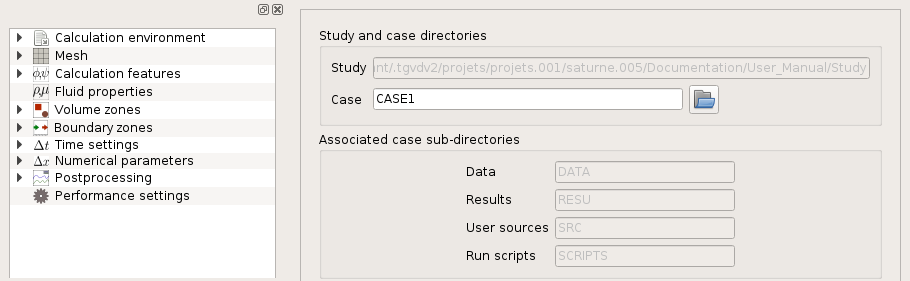
\includegraphics[width=0.9\textwidth]{gui_case_dir}
\caption{Identity and paths}
\label{fig:3_e1}
\end{center}
\end{figure}

\begin{figure}[!ht]
\begin{center}
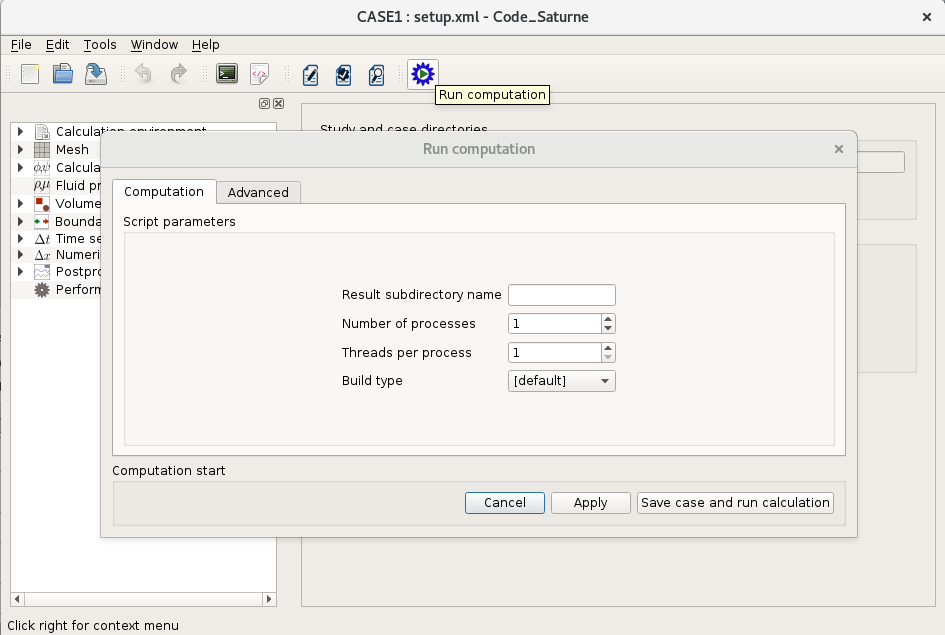
\includegraphics[width=0.9\textwidth]{gui_prepare_execution}
\caption{Prepare execution}
\label{fig:43_e1}
\end{center}
\end{figure}

If no problem arises, the simulation results can be found in the directory \texttt{CASE1/RESU} and be read directly by {\em ParaView} or {\em EnSight} in \texttt{CASE1/RESU/<YYYYMMDD-hhmm>/postprocessing}. Calculation history can be found in the file \texttt{<YYYYMMDD-hhmm>/run\_solver.log}.

%==================================
\subsection{Troubleshooting}
%==================================
If the calculation does not run properly, the user is advised to check the
following points in\\
\texttt{CASE1/RESU/<YYYYMMDD-hhmm>}:
\begin{list}{$\bullet$}{}
\item  if the calculation stops in the pre-processor, the user should check for error messages in the file \texttt{preprocessor*.log}.
\item if the problem is related to boundary conditions, the user should visualise the file \texttt{error.ensight} with {\em EnSight} or {\em ParaView},
\item if the calculation stops in the \CS core, the user should look for messages at the end of the files \texttt{run\_solver.log} and \texttt{error*}. In addition, the user can track the following keywords in the log; these are specific error signals:
  \begin{list}{-}{}
  \item  \texttt{SIGFPE}: a floating point exception occurred. It happens when there is a division by 0, when the calculation did not converge, or when a real number reached a value over $10^{300}$. Depending on the architecture \CS is running
on, this type of exception may be caught or ignored.
  \item  \texttt{SIGSEGV}: a memory error such as a segmentation violation occurred. An array may have exceeded its allocated memory size and a memory location in use was overwritten.
  \end{list}
In order to easily find the problem, it is also advised to use a debug version of \CS (see the installation documentation) in combination with the use of the valgrind tool (if it is installed). The use of valgrind can be specified in the GUI in the advanced options of the item ``Prepare batch calculation'' under the heading ``Calculation management'' or without the GUI, in the \texttt{cs\_user\_scripts.py} file (this file can be found in \texttt{DATA/REFERENCE} and should be copied in \texttt{DATA}, see \S\ref{sec:prg_stepbystepcalculation}).
\end{list}
%==================================
%==================================
\section{Practical information about \CS}
%==================================
%==================================

%==================================
\subsection{System Environment for \CS}
%==================================

%==================================
\subsubsection{Preliminary settings}
%==================================
\label{sec:prg_environementCS}

In order to use \CS, the user should define the following alias (in their \texttt{.bashrc},
or equivalent, or \texttt{.alias} file, depending on the environment):
\begin{center}
\texttt{alias cs='\$\{install\_directory\}/bin/code\_saturne'}
\end{center}
where \texttt{install\_directory} is the base directory where
\CS and its components have been installed\footnote{Without this step, using the absolute path is still possible}.

This step may be skipped if \texttt{\$\{install\_directory\}} is in a standard location (such as \texttt{/usr} or \texttt{/usr/local}.


%==================================
\subsubsection{Configuration file}
%==================================
A configuration file for \CS is available in \texttt{\$\{install\_directory\}/etc}. This file can be useful as a post-install step
for computing environments using a batch system, for separate front-end and compute systems (such as Blue Gene systems),
or for coupling with \syrthes 4 or \CA (see the installation documentation for more details).\\

A user may define a local configuration, by copying
\texttt{\$\{install\_directory\}/etc/code\_saturne.cfg} (if present)
or \texttt{\$\{install\_directory\}/etc/code\_saturne.cfg.template} to\\
\texttt{\$HOME/.code\_saturne.cfg}, then uncomment and define the applicable sections.\\

Note that this user configuration file's settings usually apply to all installed \CS versions.

Two options in the \texttt{.code\_saturne.cfg} file could be useful for the user:
\begin{list}{$\bullet$}{}
\item Set the temporary directory (see \S\ref{sec:prg_temporarydirectory} for more details on the temporary execution directory).
\item Set the mesh database directory: it is possible to indicate a path where meshes are stored.
In this case, the GUI will propose this directory automatically for mesh selection. Without the GUI, it is
then possible to fill in the \texttt{cs\_user\_scripts.py} file (see \S\ref{sec:prg_stepbystepcalculation})
with the name of the desired mesh of the database directory and the code will
find it automatically (be careful if you have the same name for a mesh in the database directory
and in the \texttt{MESH} directory, the mesh in \texttt{MESH} will be used).
\end{list}

%==================================
\subsubsection{Standard directory hierarchy}
%==================================
\label{sec:prg_architecture}%
The standard architecture for the simulation studies is:

\noindent
An optional study directory containing:
\begin{list}{$\bullet$}{}
\item A directory \texttt{MESH} containing the mesh(es)
      necessary for the study
\item A directory \texttt{POST} for the potential post-processing scripts (not
used directly by the code)
\item One or several calculation directories
\end{list}

\noindent
Every calculation directory contains:
\begin{list}{$\bullet$}{}
\item A directory \texttt{SRC} for the potential user subroutines
      necessary for the calculation
\item A directory \texttt{DATA} for the calculation data (data
      file from the interface, input profiles, thermo-chemical data, ...), the user script and the XML file.
\item A directory \texttt{SCRIPTS} for the launch script
\item A directory \texttt{RESU} for the results\\
To improve the calculation traceability, the files and directories
sent to \texttt{RESU} after a calculation are  placed in a subdirectory
named after that run's ``id'', which is by default based on the run date
and time, using the format: \texttt{YYYYMMDD-hhmm}.
It is also possible to force a specific run id, using the \texttt{--id}
option of \texttt{code\_saturne run}.
\end{list}

\noindent
In the standard cases, \texttt{RESU/<run\_id>} contains a
\texttt{postprocessing} directory with the post-processing
(visualization) files, a \texttt{restart} directory for the calculation
restart files, a \texttt{monitoring} directory for the files of chronological
record of the results at specific locations (probes),\\
\texttt{preprocessor.log} and \texttt{run\_solver.log} files reporting the
Preprocessor and the Solver execution. All files from the \texttt{DATA}
directory not in subdirectories are also copied. For a tracing of
the modifications in prior calculations, the user-subroutines used in
a calculation are stored in a \texttt{src\_saturne} subdirectory. The data files
(such as the XML Interface data file and thermo-chemical data files) and
launch script are also copied into the results directory. \texttt{compil.log} and
\texttt{summary} are respectively reports of the compilation stage and
general information on the calculation (type of machine, user,
version of the code, ...).

\begin{table}[h!t]
\begin{tabular}{lll}
\multicolumn{3}{l}{Below are typical contents of a case directory CASE1 in a study STUDY} \\
\multicolumn{2}{l}{\texttt{STUDY/CASE1/DATA:}}&{\bf \CS data}\\
&        \texttt{SaturneGUI}        &Graphical User Interface launch script\\
&        \texttt{setup.xml}         &Graphical User Interface parameter file\\
&        \texttt{REFERENCE}         &Example of user scripts and meteorological\\
&                                   &  or thermochemical date files (used with the\\
&                                   & specific physics modules)\\
\multicolumn{2}{l}{\texttt{STUDY/CASE1/SRC:}}&{\bf \CS user subroutines }\\
&        \texttt{REFERENCE}         &  Available user subroutines\\
&        \texttt{EXAMPLES}          &  Examples of user subroutines\\
&        \texttt{cs\_user\_boundary\_conditions.f90}  &  User subroutines used for the present calculation\\
&        \texttt{cs\_user\_parameters.f90} &\\
\multicolumn{2}{l}{\texttt{STUDY/CASE1/RESU/}\emph{\texttt{YYYYMMDD-hhmm:}}}&{\bf Results} for the
                                                             calculation YYYYMMDD-hhmm\\
&        \texttt{postprocessing}    &Directory containing the \CS post-processing output\\
&                                   &in the {\em EnSight}, \med, or CGNS format (both volume and boundary);\\
&        \texttt{src\_saturne}      &copy of the \CS user subroutines used for the calculation\\
&        \texttt{monitoring}        &Directory containing the chronological records for \CS\\
&        \texttt{checkpoint}        &Directory containing the \CS restart files \\
&        \texttt{compile.log}       &Compilation log\\
&     \texttt{setup.xml}            &Graphical User Interface parameter file used for the\\
&                                   &calculation\\
&        \texttt{runcase}           &Copy of the launch script used for the calculation\\
&        \texttt{preprocessor.log}  &Execution report for the \CS Preprocessor\\
&        \texttt{run\_solver.log}   &Execution report for the Solver module of \CS\\
&        \texttt{summary}           &General information (machine, user, version, ...)\\
\multicolumn{2}{l}{\texttt{STUDY/CASE1/SCRIPTS:}}&{\bf Launch script}\\
&        \texttt{runcase}           &Launch script (which may contain batch
                                     system keywords)\\
\end{tabular}
\end{table}

When running, the code
may use additional files or directories inside its execution directory, set
by the execution script, which include a \texttt{mesh\_input} file or directory,
as well as a \texttt{restart} directory (which is a link or copy of a previous
run's \texttt{checkpoint} directory), as well as a \texttt{run\_solver.sh}
script.

For coupled calculations, whether with \CS itself or \syrthes, each coupled
calculation domain is defined by its own directory (bearing the same name
as the domain), but results are placed in a \texttt{RESU\_COUPLING}
directory, with a subdirectory for each run, itself containing one
subdirectory per coupled domain. Coupled cases are run through
the standard the {\texttt{code\_saturne run} command, but require a coupling
parameters file (\texttt{coupling\_parameters.py}) specified using the
{\texttt{--coupling option}. The run command must be called from the toplevel
({\texttt{STUDY}) directory, so an additional {\texttt{STUDY/runcase} launch
script is used in this case. Note that case-local scripts (such as
{\texttt{STUDY/CASE1/SCRIPTS/runcase}) are still used by the master script to
determine which parameter file to use.

So in the coupled case, calculation results would not be placed in
\texttt{STUDY/CASE1/RESU/}\emph{\texttt{YYYYMMDD-hhmm}}, but in
\texttt{STUDY/RESU\_COUPLING/}\emph{\texttt{YYYYMMDD-hhmm}}\texttt{/CASE1}, with the \texttt{summary}
file being directly placed in \texttt{STUDY/RESU\_COUPLING/}\emph{\texttt{YYYYMMDD-hhmm}}
(as it references all coupled domains).

\begin{table}[h!t]
\begin{tabular}{lll}
\multicolumn{3}{l}{Below are typical additional contents with a coupled \syrthes
  case SOLID1 in a study STUDY} \\
\multicolumn{2}{l}{\texttt{STUDY/runcase}}&{Coupled launch script}\\
\multicolumn{2}{l}{\texttt{STUDY/coupling\_parameters.py}}&{Coupled launch parameters}\\
\multicolumn{2}{l}{\texttt{STUDY/SOLID1/DATA:}}&{\bf \syrthes data}\\
&        \texttt{syrthes\_data.syd}          &\syrthes data file \\
&        \texttt{syrthes.py}                 &\syrthes script\\
&        \texttt{usr\_examples}              &\syrthes user subroutine examples\\
\multicolumn{2}{l}{\texttt{STUDY/RESU\_COUPLING/}\emph{\texttt{YYYYMMDD-hhmm}}\texttt{/SOLID1:}}&{\bf results
 (file names defined in \texttt{syrthes.env})}\\
&        \texttt{src}                &\syrthes user subroutines
                                     used in the calculation\\
&        \texttt{compile.log}        &\syrthes compilation report\\
&        \texttt{listsyr}            &Execution log\\
&        \texttt{geoms}              &\syrthes \ solid geometry file\\
&        \texttt{histos1}            &\syrthes chronological records at
                                               specified monitoring points\\
&        \texttt{resus1}             &\syrthes calculation restart file (1 time step)\\
&        \texttt{resusc1}            &\syrthes chronological solid
                                      post-processing file\\
&                                    &(may be transformed into the {\em EnSight}\\
&                                    & or {\em MED} format with the {\em syrthes4ensight}\\
&                                    & or {\em syrthes4med30} utility)\\
\end{tabular}
\end{table}

%==================================
\subsubsection{\CS Solver library files}
%==================================
\label{sec:prg_library}%
Information about the content of the \CS base directories is given below. It
is not of vital interest for the user, but given only as general
information. Indeed, the case preparer command \texttt{code\_saturne~create}
automatically extracts the necessary files and prepares the launch script
without the user having to go directly into the \CS base directories
(see \S\ref{sec:prg_cscreate}).
The \texttt{code\_saturne~info} command gives direct
access to the most needed information (especially the user's and theory
guides and the Doxygen documentation) without the user having to look for them in the \CS
directories.

The subdirectories \texttt{\{install\_directory\}/lib} and \texttt{\{install\_directory\}/bin }
contain the libraries and compiled executables respectively.

The data files (for instance thermochemical data) are located in the
directory \texttt{data}.

The user subroutines are available in the directory \texttt{src/user},
with examples in \texttt{src/user\_examples}.
The case preparer command \texttt{code\_saturne~create} copies all these files
in the user directories \texttt{SRC/REFERENCE} and \texttt{SRC/EXAMPLES}
during the case preparation.

The directory \texttt{bin} contains an example of the launch script, the
compilation parameter files and various utility programs.

%==================================
\subsection{Setting up and running a calculation}
%==================================

%==================================
\subsubsection{Step by step calculation}
%==================================
\label{sec:prg_stepbystepcalculation}%

This paragraph summarises the different steps which are necessary to
prepare and run a standard case:

\begin{list}{$\bullet$}{}

\item Check the version of \CS set for use in the environment variables
(\texttt{code\_saturne~info --version}). If it does not correspond to
the desired version, update the user profile or aliases to get the
required version, logging out of the session and in again if necessary (cf.
\S\ref{sec:prg_environementCS}).

\item Prepare the different directories using the \texttt{code\_saturne~create}
command (see \S\ref{sec:prg_cscreate}).

\item It is recommended to place the mesh(es) in the directory \texttt{MESH},
but they may be selected from other directories, either with the Graphical User Interface (GUI)
 or the \texttt{cs\_user\_scripts.py} file (see below). Make sure they are
in a format compliant with \CS (see \S\ref{sec:prg_meshes}). There can be
several meshes in case of mesh joining or coupling with
\syrthes\footnote{\syrthes 4 uses meshes composed of 4-node tetrahedra}.

\item Go to the directory \texttt{DATA} and launch the
      GUI using the command \texttt{./SaturneGUI}.

\item If not using the GUI, copy the
  \texttt{DATA/REFERENCE/cs\_user\_scripts.py} file to \texttt{DATA} and
  edit it, so that the correct run options and paths may be set. For advanced
  uses, this file may also be used in conjunction with the GUI. Just as with
  user Fortran subroutines below, settings defined in this file have priority
  over those defined in the GUI.

\item Place the necessary user subroutines in the directory \texttt{SRC} (see
\S\ref{sec:prg_ssprgutilis}). When not using the Interface, some subroutines are
compulsory.

\begin{list}{}{}

\item {\bf For all physics:}

    \begin{list}{}{}
        \item {\em compulsory without Graphical User Interface:}
        \begin{list}{-}{}
            \item \texttt{usipph} (in \texttt{cs\_user\_parameters.f90}) to
              specify the turbulence and temperature models

            \item \texttt{usipsu} (in \texttt{cs\_user\_parameters.f90}) to
              define most user parameters

            \item \texttt{cs\_user\_boundary\_conditions} to manage the boundary conditions
        \end{list}

        \item {\em  very useful without Graphical User Interface:}
        \begin{list}{-}{}
            \item \texttt{\texttt{cs\_user\_model.c}}
              (in \texttt{cs\_user\_parameters.c}) to
              define user scalars (species)

            \item \texttt{usipes} (in \texttt{cs\_user\_parameters.f90}) to
              define monitoring points and additional parameters for results outputs
        \end{list}

        \item {\em  very useful:}
        \begin{list}{-}{}
            \item \texttt{usphyv} (in
              \texttt{cs\_user\_physical\_properties.f90}) to manage variable physical
                  properties (fluid density, viscosity ...)

            \item \texttt{cs\_user\_initialization} to manage the non-standard initialisations
        \end{list}
    \end{list}

  \item{\bf For the ``gas combustion'' specific physics:}

    \begin{list}{}{}
        \item {\em compulsory without Graphical User Interface:}
        \begin{list}{-}{}
            \item \texttt{usppmo} (in \texttt{cs\_user\_parameters.f90})
               to select a specific physics module and combustion model
        \end{list}

        \item {\em very useful:}
        \begin{list}{-}{}
            \item  \texttt{cs\_user\_combustion}
                   (in \texttt{cs\_user\_parameters.f90}),
                   depending on the selected combustion model,
                   to specify the calculation options
                   for the variables
                   corresponding to combustion model
        \end{list}
    \end{list}

  \item{\bf For the ``pulverized fuel combustion'' specific physics:}

    \begin{list}{}{}
        \item {\em compulsory without Graphical User Interface:}
        \begin{list}{-}{}
            \item \texttt{usppmo} (in \texttt{cs\_user\_parameters.f90})
               to select the specific physics module
        \end{list}

        \item {\em very useful:}
        \begin{list}{-}{}
            \item  \texttt{cs\_user\_combustion}
               (in \texttt{cs\_user\_parameters.f90})
               to specify the calculation options
                   for the variables
                   corresponding to pulverized fuel combustion
        \end{list}
    \end{list}

or \texttt{cs\_user\_combustion}
  \item{\bf For the ``heavy fuel combustion'' specific physics:}

 (not accessible through the Graphical User Interface in version \verscs)
    \begin{list}{}{}
        \item {\em compulsory:}
        \begin{list}{-}{}
            \item \texttt{usppmo} (in \texttt{cs\_user\_parameters.f90})
               to select the specific physics module
            \item \texttt{cs\_user\_combustion}
               (in \texttt{cs\_user\_parameters.f90})
               to specify the calculation options
                   for the variables
                   corresponding to heavy fuel combustion
        \end{list}
    \end{list}


     \item{\bf For the ``atmospheric module'' specific physics:}

    \begin{list}{}{}
       \item {\em compulsory without Graphical User Interface:}
        \begin{list}{-}{}
            \item \texttt{usppmo} (in \texttt{cs\_user\_parameters.f90})
                  to select the specific physics module
        \end{list}

        \item {\em very useful:}
        \begin{list}{-}{}
            \item  \texttt{usati1} (in \texttt{cs\_user\_parameters.f90})
                   to manage the reading of the meteo file
           \item  \texttt{usadtv} or \texttt{usatsoil} (in \texttt{cs\_user\_atmospheric\_model.f90})
                   to manage the options to the specific physics

        \end{list}
    \end{list}


     \item{\bf For the ``electric module'' specific physics
      (Joule effect and electric arcs):}

    \begin{list}{}{}
       \item {\em compulsory without Graphical User Interface:}
        \begin{list}{-}{}
            \item \texttt{usppmo} (in \texttt{cs\_user\_parameters.f90})
                  to select the specific physics module

            \item \texttt{cs\_user\_initialization} to initialise the enthalpy in
                  case of Joule effect

            \item \texttt{cs\_user\_physical\_properties.c}
                  to define the physical
                  properties in case of Joule effect
        \end{list}

        \item {\em very useful:}
        \begin{list}{-}{}
            \item  \texttt{cs\_user\_model} and \texttt{cs\_user\_parameters} (in \texttt{cs\_user\_parameters.c})
                   to manage the options related
                   to the variables corresponding to the electric module

        \end{list}
    \end{list}

%     \item{\bf For the ``heavy fuel oil combustion module'' specific physics:}
%(not accessible through the Graphical User Interface in version \verscs)
%    \begin{list}{}{}
%        \item {\em compulsory:}
%        \begin{list}{-}{}
%            \item \texttt{usppmo} to select the specific physics module
%        \end{list}
%    \end{list}


    \item{\bf For the ``Lagrangian module'' (dispersed phase):}

(the continuous phase is managed in the same way as for a case of standard
physics)
    \begin{list}{}{}
        \item {\em compulsory without Graphical User Interface:}
        \begin{list}{-}{}
            \item \texttt{cs\_user\_lagr\_model} to manage the calculation conditions

            \item \texttt{cs\_user\_lagr\_boundary\_conditions} to manage the
              boundary conditions for the dispersed phase

        \end{list}

    \end{list}

   \item {\bf For the ``compressible module'':}

    \begin{list}{}{}
        \item {\em compulsory without Graphical User Interface:}
        \begin{list}{-}{}
            \item \texttt{usppmo} (in \texttt{cs\_user\_parameters.f90})
                  to select the specific physics module
        \end{list}
        \item {\em very useful:}
        \begin{list}{-}{}
            \item \texttt{uscfx1} and \texttt{uscfx2} (in \texttt{cs\_user\_parameters.f90})
                  to manage the calculation parameters

%            \item \texttt{cs\_user\_boundary\_conditions} to manage the
%                  boundary conditions

           \item \texttt{usphyv} (in \texttt{cs\_user\_physical\_properties}
                  to manage the variable physical properties

        \end{list}
    \end{list}

\end{list}


A comprehensive list of the user subroutines and their instructions
      for use are given in \S\ref{sec:prg_ssprgutilis}.

\item If necessary, place in the directory \texttt{DATA} the different
      external data (input profiles, thermochemical data files, ...)

\item Prepare the launch script \texttt{runcase}, directly or through the
      Graphical Interface (see \S\ref{sec:prg_runcase}), or prepare the
      \texttt{DATA/cs\_user\_scripts.py} file.

\item Run the calculation and analyse the results

\item If necessary, purge the temporary files (in \texttt{RESU/<run\_id>} or
      \texttt{<scratch>/<run\_id>} directory) (see \S\ref{sec:prg_temporarydirectory}).
\end{list}


%==================================
\subsubsection{Temporary execution directory}
%==================================
\label{sec:prg_temporarydirectory}%
During a calculation, \CS may use a temporary directory for the compilation and
the execution if such a ``scratch'' directory is defined in the GUI, by setting the
\texttt{CS\_SCRATCHDIR} environment variable, or in the \texttt{code\_saturne.cfg} file.
In this case, it is only at the end of the compilation that the result files are only copied at the end in the directory
\texttt{RESU}. This is recommended if the compute environment includes different
file-systems, some better suited to data storage, others to intensive I/O.
If this is not the case, there is no point in running in a scratch directory
rather than the results directory, as this incurs additional file copies.

If the environment variable \texttt{CS\_SCRATCHDIR} is defined,
its value has priority over that defined in the preference file
so if necessary, it
is possible to define a setting specific to a given run using this mechanism.

\noindent
{\em WARNING: in case of an error, the temporary directories are not deleted
after a calculation, so that they may be used for debugging. They may then
accumulate and may hinder the correct operation of the machine.\\
\centerline{\bf It is therefore essential to remove them regularly.}}


%==================================
\subsubsection{Execution modes}
%==================================
\label{sec:prg_executionmodes}%
As explained before, \CS is composed of two main modules, the Preprocessor and the
Solver. The Preprocessor reads the meshes.
The resulting data is transferred to the Solver through specific
files, named \texttt{mesh\_input}, or placed in a directory of that name when
multiple meshes are imported.

Yet, the Preprocessor does not run in parallel and may require a
large amount of memory. The launch scripts therefore allows specifically
choosing which modules to run, either through the GUI or through the
\texttt{cs\_user\_scripts.py} file:

\hspace*{0.5cm} If a {mesh\_input} file or directory is defined (which may be
either a {mesh\_input} from a previous Preprocessor run or a {mesh\_output}
from a previous solver run), the script will copy or link it to
the execution directory, and the Preprocessor will not be rerun.

\hspace*{0.5cm} If \texttt{domain.exec\_kernel = False}, the Solver will not
be run. This is useful when only the mesh import stage is required.

In a similar manner, the Solver accepts several command-line options relative to execution mode, notably \texttt{domain.solver\_args = '--preprocess'} or \texttt{'--quality'}, restricting the run to the preprocessing stages, or preprocessing stages augmented by mesh quality criteria computation. Whenever the preprocessing stages defined lead to an effective mesh modification, a \texttt{mesh\_output} file is produced, which can be used directly as an input for a successive calculation.

The GUI presents the range of options in the form of four execution modes (under the ``Mesh`` page):

\begin{list}{$\bullet$}{}

\item {\bf mesh import}: the Preprocessor is run to transform one or more meshes into an internal \texttt{mesh\_input} file (or directory in case of multiple meshes).

\item {\bf mesh preprocessing}: the Solver is run in preprocessing mode, so as to handle all mesh modification operations, such as joining, periodicity, smoothing, \emph{etc.} If a \texttt{mesh\_input} file or directory is provided, it is used directly; otherwise, mesh import is run first.

\item {\bf mesh quality criteria}: similar to preprocessing, with the addition of mesh quality criteria computation, and post-processing output of those criteria. Some additional mesh consistency checks are also run.

\item {\bf standard}: this includes preprocessing, followed by a standard computation.

\end{list}

Note that to allow preprocessing in multiple passes, all defined preprocessing operations are run even on previously preprocessed meshes. In most cases, those will not produce additional changes (such as joining already joined meshes), but in the case of mesh smoothing, they might lead to small changes. So when using a previously preprocessed mesh it is recommended
not to define any preprocessing operations, so as to skip the preprocessing stage.

It is encouraged to separate the preprocessing and calculation runs, as
this not only speeds up calculations, but also ensures that the mesh is identical, regardless of the architecture or number of processors it is run on. Indeed, when running the same pre-processing stages such as mesh joining on a different machine or a different number of processors, very minor floating-point truncation errors may lead to very slightly different preprocessed meshes.
The GUI option to ``Use unmodified checkpoint mesh in case of restart`` encourages this usage.

Note also that mesh partitioning is done directly by the Solver.
Depending on the partitioning algorithm used, a partition map
(\texttt{partition\_output/domain\_number\_*}) may be output,
allowing the use of the same partitioning in future calculations.
By default, this file is output when using graph-based partitioners, which may
use randomization and do not guarantee a reproducible output, and is not output
when using a deterministic space-filling curve based partitioning.

If the code was built only with a serial partitioning library,
graph-based partitioning may best be run in a serial pre-processing stage.
In some cases, serial partitioning might also provide better partitioning
quality than parallel partitioning, so if both are available, comparing
the performance of the code may be worthwhile, at least for calculations
expected to run for many iterations.

%==================================
\subsubsection{Environment variables\label{sec:envcs}}
%==================================

Setting a few environment variables specific to \CS allows modifying
its default behaviour. The environment variables used by \CS
are described here:

\envvar{CS\_SCRATCHDIR}

Allows defining the execution directory (see
\S\ref{sec:prg_temporarydirectory}),
overriding the default path or settings from the global
or user \texttt{code\_saturne.cfg}.

\envvar{CS\_MPIEXEC\_OPTIONS}

This variable allows defining extra arguments to be passed to
the MPI execution command by the run scripts.
If this option is defined, it will have priority over the value defined
in the preference file (or by computed defaults), so if necessary, it
is possible to define a setting specific to a given run using this
mechanism. This may be useful when tuning the installation to a given
machine, for example experimenting MPI mapping and ``bind to core''
features.

%==================================
\subsubsection{Interactive modification of selected parameters}
%==================================
\label{sec:prg_control_file}%
During a calculation, it is possible to change the limit time step number
(\texttt{ntmabs}) specified through the GUI or in \texttt{cs\_user\_parameters.f90}.
To do so, a file named \texttt{control\_file} must be placed in the
execution directory (see \S\ref{sec:prg_temporarydirectory}).
The existence of this file is checked at the beginning of each time step.

To change the maximum number of time steps, this file must contain a line
indicating the value of the new limit number of time steps.\\
If this new limit has already been reached,
 \CS will stop
properly at the end of the current time step (the results and restart files
will be written correctly).\\
This procedure allows the user to stop a calculation in a clean and interactive
way whenever they wish.

The \texttt{control\_file} may also contain a few other commands,
allowing the user to force checkpointing or postprocessing at a given time step
or physical time, or to force an update of log files.
The following commands are available (using the common notations $< >$ to
indicate a required argument, $[ ]$ to indicate an optional argument).

\begin{tabular}[top]{|p{6.5cm}%
                     |>{\PreserveBackslash\raggedright\hspace{0pt}}p{8.5cm}|}
\hline
\texttt{max\_time\_step}                   & $<$time\_step\_number$>$ \\
\texttt{max\_time\_value}                  & $<$time\_value$>$ \\
\texttt{max\_wall\_time}                   & $<$wall\_time$>$ \\
\hline
\texttt{checkpoint\_time\_step}            & $<$time\_step\_number$>$ \\
\texttt{checkpoint\_time\_value}           & $<$time\_value$>$ \\
\texttt{checkpoint\_wall\_time}            & $<$wall\_clock\_time$>$ \\
\texttt{checkpoint\_time\_step\_interval}   & $<$time\_step\_interval$>$ \\
\texttt{checkpoint\_time\_value\_interval}  & $<$time\_interval$>$  \\
\texttt{checkpoint\_wall\_time\_interval}   & $<$wall\_time\_interval$>$ \\
\hline
\texttt{control\_file\_wtime\_interval}     & $<$wall\_time\_interval$>$ \\
\hline
\texttt{flush}                             & $[$time\_step\_number$]$ \\
\hline
\hline
\texttt{notebook\_set}                     & $<$parameter\_name$>$ $<$value$>$ \\
\hline
\texttt{postprocess\_time\_step}           & $<$time\_step\_number$>$ [writer\_id] \\
\texttt{postprocess\_time\_value}          & $<$time\_step\_value$>$ [writer\_id] \\
\hline
\texttt{time\_step\_limit}                 & $<$time\_step\_count$>$ \\
\hline
\end{tabular}

The \texttt{time\_step\_limit} differs from the \texttt{max\_time\_step} command,
in the sense that it allows reducing the maximum number of time steps,
but not increasing it. Also, in the case of a restart, it refers to the
number of additional time steps, not to the number of absolute time steps.

Note that for the \texttt{postprocess\_time\_*} options, the last argument
(\texttt{writer\_id}} is optional. If not defined, or 0, postprocessing
is activated for all writers; if specified, only the writer with the specified
id is affected. Also, postprocessing output by one ore more writers at a
future time step may be cancelled using the negative value of that time step.

For the \texttt{flush} option, the time step is also optional. If not
specified, logs and time plots are updated at the beginning of the
next time step. Also, if the \texttt{control\_file} is empty (such as
when created by the \texttt{touch control\_file} command on Unix/Linux
systems, a \texttt{flush} request for the next time step.

Multiple entries may be defined in this file, with one line per entry.

%==================================
\subsection{Case preparer}
%==================================
\label{sec:prg_cscreate}%
The case preparer command \texttt{code\_saturne~create} automatically creates a
study directory according to the typical architecture and copies and
pre-fills an example of calculation launch script.

The syntax of \texttt{code\_saturne~create} is as follows:

\noindent
\texttt{code\_saturne~create --study STUDY CASE\_NAME1 CASE\_NAME2...}\\
creates a study directory \texttt{STUDY} with case subdirectories
\texttt{CASE\_NAME1} and \texttt{CASE\_NAME2}...
If no case name is given, a default case directory called \texttt{CASE1} is
created.

\noindent
\texttt{code\_saturne~create --case Flow3 --case Flow4}\\
executed in the directory \texttt{STUDY} adds the case directories
\texttt{Flow3} and \texttt{Flow4}. Whenever multiple cases are created simultaneously, it is assumed they may be coupled, so toplevel \texttt{runcase} and \texttt{coupling\_parameters.py} files and \texttt{RESU\_COUPLING} directory are also created.

In the directory \texttt{DATA}, the \texttt{code\_saturne~create} command
places a subdirectory \texttt{REFERENCE} containing examples of thermochemical
data files used for pulverised coal combustion, gas combustion, electric arcs, or
a meteo profile. The file to be used for the calculation must be copied directly
in the \texttt{DATA} directory and its name may either be unchanged, or
be referenced using the GUI or using the \texttt{usppmo} subroutine in
\texttt{cs\_user\_parameters.f90}. As a rule of thumb, all files in \texttt{DATA}
except for \texttt{SaturneGUI} are copied, but subdirectories are not.\\
The \texttt{code\_saturne~create} command also places in the directory
\texttt{DATA} the launch script for the Graphical User Interface:
\texttt{SaturneGUI}.

In the directory \texttt{SRC}, the \texttt{code\_saturne~create} command creates a
subdirectory \texttt{REFERENCE} containing all the available user subroutines,
and the subdirectory \texttt{EXAMPLES} containing examples of user subroutines.
Only the user subroutines placed directly under
the directory \texttt{SRC} will be considered. The others will be ignored.

In the directory \texttt{SCRIPTS}, the \texttt{code\_saturne~create} command copies an example of the launch script: \texttt{runcase}.
The XML file may be specified in the script (see \S\ref{sec:prg_runcase}),
and using the GUI sets it automatically.

\smallskip \noindent

%==================================
\subsection{Supported mesh and post-processing output formats
\label{sec:formats}}
%==================================

\CS supports multiple mesh formats, all of these having been requested
at some time by users or projects based on their meshing or post-processing
tools. All of these formats have advantages and disadvantages (in terms
of simplicity, functionality, longevity, and popularity) when compared to
each other. The following formats are currently supported by \CS:

\begin{list}{-}{}

\item \hyperref[sec:fmtdesc_des]{\simail (NOPO)}
\item \hyperref[sec:fmtdesc_unv]{\ideas universal}
\item \hyperref[sec:fmtdesc_med]{\med}
\item \hyperref[sec:fmtdesc_cgns]{CGNS}
\item \hyperref[sec:fmtdesc_ensight6]{\ensight 6}
\item \hyperref[sec:fmtdesc_ensightg]{\ensightg}
\item \hyperref[sec:fmtdesc_neu]{\gambit neutral}
\item \hyperref[sec:fmtdesc_gmsh]{\gmsh}
\item \hyperref[sec:fmtdesc:ccm]{STAR-CCM+}
\item \hyperref[sec:fmtdesc_catalyst]{\catalyst (co-processing)}
\end{list}

These formats are described in greater detail in the following sections.
Unless a specific option is used, the \pcs determines the mesh format directly
from the file suffix: %
{\em``\texttt{.case}''} for \ensight (6 or Gold),
{\em``\texttt{.ccm}''} for STAR-CCM+,
{\em``\texttt{.cgns}''} for CGNS,
{\em``\texttt{.des}''} for \simail,
{\em``\texttt{.med}''} for \med,
{\em``\texttt{.msh}''} for \gmsh,
{\em``\texttt{.neu}''} for \gambit neutral,
{\em``\texttt{.unv}''} for I-deas universal.

Note that the preprocessor can read gzipped mesh files directly (for Formats
other than MED or CGNS, which use specific external libraries) on most machines.

%==================================
\subsubsection{Formats supported for input\label{sec:formats_in}}
%==================================

\subsubsubsection{NOPO/\simail (INRIA/Distene)%
\label{sec:fmtdesc_des}}

This format is output by \simail, which was used heavily at EDF until
a few years ago. \CS does not
currently handle cylindrical or spherical coordinates, but it seems that
\simail always outputs meshes in Cartesian coordinates, even if points
have been defined in another system. Most ``classical'' element types
are usable, except for pyramids.

Note that depending on the architecture on which a file was
produced by \simail\footnote{``little endian'' on Intel or AMD processors, or
``big endian'' on most others, and starting with \simail 7, 32-bit or 64-bit
 integer and floating-point numbers depending on architecture},
it may not be directly readable by \simail on a different machine, while
this is not a problem for the \pcs, which automatically detects the
byte ordering and the 32/64 bit variant and adjusts accordingly.

\smallskip \noindent
\begin{tabular}[top]{|p{4.5cm}%
                     |>{\PreserveBackslash\raggedright\hspace{0pt}}p{10.5cm}|}
\hline
Default extension: & {\tt .des}\\
\hline
File type:         & semi-portable ``Fortran'' binary (IEEE integer and
                     floating-point numbers on 4 or 8 bytes, depending on
                     32 or 64 bit \simail version, bytes also ordered based
                     on the architecture)\\
\hline
Surface elements:  & triangles, quadrangles
                     (+ volume element face references)\\
\hline
Volume elements:   & tetrahedra, prisms, hexahedra\\
\hline
Zone selection:    & element face references and volume sub-domains\\
                   & (interpreted as numbered groups)\\
\hline
Compatibility:     & all files of this type as long as the coordinate
                     system used is Cartesian and not cylindrical or
                     spherical\\
\hline
Documentation:     & Simail user documentation and release notes or
                     MODULEF documentation:
                     \url{http://www-rocq.inria.fr/modulef} \par
                     Especially: \par
                     \url{http://www-rocq.inria.fr/modulef/Doc/FR/Guide2-14/node49.html} \\
\hline
\end{tabular}

\subsubsubsection{\ideas universal file%
\label{sec:fmtdesc_unv}}

This format was very popular in the 1990's and early 2000's, and though
the I-deas tool has not focused on the CFD (or even meshing) market since
many years, it is handled (at least in part) by many tools, and may
be considered as a major ``legacy'' format. It may contain many different
datasets, relative to CAD, meshing, materials, calculation results,
or part representation. Most of these datasets are ignored by \CS,
and only those relative to vertex, element, group, and coordinate system
definitions are handled.

This format's definition evolves with \ideas versions, albeit in a limited
manner: some datasets are declared obsolete, and are replaced by others,
but the definition of a given dataset type is never modified. Element and
Vertex definitions have not changed for many years, but group definitions
have gone through several dataset variants through the same period,
usually adding minor additional group types not relevant to meshing.
If one were to read a file generated with a more recent version of \ideas
for which this definitions would have changed with no update in the \pcs,
as the new dataset would be unknown, it would simply be ignored.

Note that this is a text format. Most element types are handled, except
for pyramids.

\smallskip \noindent
\begin{tabular}[top]{|p{4.5cm}%
                     |>{\PreserveBackslash\raggedright\hspace{0pt}}p{10.5cm}|}
\hline
Default extension: & {\tt .unv}\\
\hline
File type:         & text\\
\hline
Surface elements:  & triangles, quadrangles\\
\hline
Volume elements:   & tetrahedra, prisms, hexahedra\\
\hline
Zone selection:    & colors (always) and named groups\\
\hline
Compatibility:     & \ideas (\emph{Master Series} 5 to 9, \emph{NX Series} 10 to 12)
                     at least\\
\hline
Documentation:     & Online I-deas NX Series documentation, and\\
                     \url{https://docs.plm.automation.siemens.com/tdoc/nx/10/nx_help/#uid:index_advanced:xid602249:id625716:id625821}\\
\hline
\end{tabular}

\subsubsubsection{\gambit neutral%
\label{sec:fmtdesc_neu}}

This format may be produced by Ansys \fluent's GAMBIT meshing tool.
As this tool does not export meshes to other formats directly handled
by the \pcs (though \fluent itself may export files to the CGNS or
\ideas universal formats), it was deemed useful to enable the \pcs
to directly read files in \gambit neutral format.

Note that this is a text format. ``Classical'' element types are usable.

\smallskip \noindent
\begin{tabular}[top]{|p{4.5cm}%
                     |>{\PreserveBackslash\raggedright\hspace{0pt}}p{10.5cm}|}
\hline
Default extension: & {\tt .neu}\\
\hline
File type:         & text\\
\hline
Surface elements:  & triangles, quadrangles\\
\hline
Volume elements:   & tetrahedra, pyramids, prisms, hexahedra\\
\hline
Zone selection:    & boundary conditions for faces, element groups for cells\\
                   & (interpreted as named groups)\\
\hline
Documentation:     & GAMBIT on-line documentation\\
\hline
\end{tabular}

\subsubsubsection{\ensight 6%
\label{sec:fmtdesc_ensight6}}

This format is used for output by the \harpoon meshing tool, developed
by Sharc Ltd (also the distributor of \ensight for the United Kingdom).
This format may represent all ``classical'' element types.

Designed for post processing, it does not explicitly handle the definition
of surface patches or volume zones, but allows the use of many \emph{parts}
(i.e. groups of elements) which use a common vertex list.
A possible convention (used at least by \harpoon) is to add surface
elements to the volume mesh, using one \emph{part} per group. The volume
mesh may also be separated into several \emph{parts} so as to identify
different zones. As \emph{part} names may contain up to 80 characters,
we do not transform them into groups (whose names could be unwieldy),
so we simply convert their numbers to group names.

Also note that files produced by \harpoon may contain badly oriented
prisms, so the \pcs orientation correction option
(\texttt{--reorient}) may must be used. Meshes built by this tool also
contain hanging nodes, with non-conforming elements sharing some vertices.
Mesh joining must thus also be used, and is not activated automatically,
as the user may prefer to specify which surfaces should be joined,
and which ones should not (\textit{i.e.} to conserve thin walls).

\smallskip \noindent
\begin{tabular}[top]{|p{4.5cm}%
                     |>{\PreserveBackslash\raggedright\hspace{0pt}}p{10.5cm}|}
\hline
Default extension: & {\tt .case}\\
\hline
File type:         & text file (extension \emph{.case}), and text,
                     binary, or Fortran binary file with
                     (\emph{.geo} extension), describing integers and floats in the IEEE format,
                     using 32 bits\\
\hline
Surface elements:  & triangles, quadrangles\\
\hline
Volume elements:   & tetrahedra, pyramids, prisms, hexahedra\\
\hline
Zone selection:    & part numbers interpreted as numbered groups\\
\hline
Compatibility:     & All files of this type\\
\hline
Documentation:     & on-line documentation, also available at:
                     \url{www3.ensight.com/EnSight10_Docs/UserManual.pdf}\\
\hline
\end{tabular}

\subsubsubsection{\gmsh%
\label{sec:fmtdesc_gmsh}}

This format is used by the free \href{http://www.geuz.org/gmsh}{\gmsh}
tool. This tool has both meshing and post-processing functionality,
but \CS only imports the meshes.

Note that some meshes produced by \gmsh man contain some badly oriented
elements, so the \pcs's \texttt{-reorient} option may be necessary.

The \pcs handles versions 1 and 2 of this array. In version 1,
two labels are associated with each element: the first defines the
element's physical entity  number, the second defines its elementary
entity number. Using version 2, it is possible to associate an
arbitrary number of labels with each element, but files produced
by \gmsh use 2 labels, with the same meanings as with version 1.

The decision was taken to convert physical entity numbers to groups. It is possible
to build a mesh using \gmsh without defining any  physical entities
(in which case all elements will belong to the same group, but the \gmsh
documentation clearly says that geometric entities are to be used
so as to group elementary entities having similar ``physical'' meanings.

To obtain distinct groups with a mesh generated by \gmsh, it
is thus necessary for the user to define physical entities.
This requires an extra step, but allows for fine-grained control
over the groups associated with the mesh, while using only elementary
entities could lead to a high number of groups.

\smallskip \noindent
\begin{tabular}[top]{|p{4.5cm}%
                     |>{\PreserveBackslash\raggedright\hspace{0pt}}p{10.5cm}|}
\hline
Default extension: & {\tt .msh}\\
\hline
File type:         & text or binary file\\
\hline
Surface elements:  & triangles, quadrangles\\
\hline
Volume elements:   & tetrahedra, pyramids, prisms, hexahedra\\
\hline
Zone selection:    & physical entity numbers interpreted as numbered groups\\
\hline
Compatibility:     & all files of this type\\
\hline
Documentation:     & included documentation, also available at:
                     \href{http://www.geuz.org/gmsh}
                          {http://www.geuz.org/gmsh}\\
\hline
\end{tabular}

%==================================
\subsubsection{Formats supported for input or output\label{sec:formats_inout}}
%==================================

\subsubsubsection{\ensightg%
\label{sec:fmtdesc_ensightg}}

This format may represent all ``classical'' element types, as well as
arbitrary polygons and convex polyhedra.

This format evolves slightly from one \ensight version to another, keeping
backwards compatibility. For example, polygons could not be used in the
same \emph{part} as other element types prior to version 7.4, which removed
this restriction and added support for polyhedra. Version 7.6 added support
for material type definitions.

This format offers many possibilities not used by \CS, such as defining
values on part of a mesh only (using ``undefined'' marker values or
partial values), assigning materials to elements, defining rigid
motion, or defining per-processor mesh parts with ghost cells for
parallel runs. Note that some libraries allowing direct \ensightg support
do not necessarily support the whole format specification.
Especially, VTK does not support material types.
Also, both \ensightg (8.2 and above) and VTK allow for automatic distribution,
reducing the usefulness of pre-distributed meshes with per-processor files.

Note than when using \paraview, if multiple parts (i.e. meshes) are
present in a give case, using the ``Extract Blocks'' filter is
required to separate those parts and obtain a proper visualization,
unless the \texttt{separate\_meshes} writer option is used.
The VisIt software does not seem to handle multiple parts in an \ensight case,
so different meshes must be assigned to different \emph{writers},
or the \texttt{separate\_meshes} option must be used
(see \S\ref{sec:prg_definitionpostprocess}) when using this tool.

This format may be used as an input format, similar to \ensight 6.
Compared to the latter, each \emph{part} has its own coordinates and vertex
connectivity; hence as a convention, we consider that surface or
volume zones may only be considered to be part of the same mesh
if the file defines vertex IDs (which we consider to be
unique vertex labels). In this case, \emph{part} numbers
are interpreted as group names. Without vertex IDs, only one part is read,
and no groups are assigned.

\smallskip \noindent
\begin{tabular}[top]{|p{4.5cm}%
                     |>{\PreserveBackslash\raggedright\hspace{0pt}}p{10.5cm}|}
\hline
Default extension: & {directory {\tt{{\it \{case\_name\}}.ensight}},
                     containing a file with the \tt .case} extension\\
\hline
File type:         & multiple binary or text files\\
\hline
Surface elements:  & triangles, quadrangles, polygons\\
\hline
Volume elements:   & tetrahedra, pyramids, prisms, hexahedra, convex polyhedra\\
\hline
Zone selection:    & possibility of defining element materials (not used), or
                     interpret part number as group name if vertex IDs are
                     given\\
\hline
Compatibility:     & files readable by \ensight 7.4 to 10.0, as well as tools
                     based on the \href{http://www.vtk.org}{\vtk} library,
                     especially \paraview\ (\url{http://www.paraview.org})\\
\hline
Documentation:     & online documentation, also available at:
                     \url{www3.ensight.com/EnSight10_Docs/UserManual.pdf}\\
\hline
\end{tabular}

\subsubsubsection{\med}\hyperdef{sec}{med}{}
\label{sec:fmtdesc_med}

Initially defined by EDF R\&D, this format (\emph{Mod\`ele d'\'echanges de Donn\'ees},
or \emph{Model for Exchange of Data}) has been defined and maintained through
a \med working group comprising members of EDF R\&D and CEA.
This is the reference format for the
\href{http://www.salome-platform.org/}{\emph SALOME} environment.
This format is quite complete, allowing the definition of all ``classical''
element types, in nodal or descending connectivity.
It may handle polygonal faces and polyhedral cells,
as well as the definition of structured meshes.

This format, which requires a library also depending on the free HDF5 library,
allows both for reading and writing meshes with their attributes (``families'' of
group combinations), as well as handling calculation data,
with the possibility (unused by \CS) of defining variables only on a subset
(``profile'') of a mesh.

The \med library is available under a \href{http://www.gnu.org}{LGPL} license,
and is even packaged in some Linux distributions
(at least Debian and Ubuntu). \CS requires at least \med 3.0.2, which in turn
requires HDF5 1.8. This format is upwards-compatible with \med 2.3,
so old files in that version of the format may be read, though not output.

\smallskip \noindent
\begin{tabular}[top]{|p{4.5cm}%
                     |>{\PreserveBackslash\raggedright\hspace{0pt}}p{10.5cm}|}
\hline
Default extension:    & {\tt .med}\\
\hline
File type:            & portable binary, based on the HDF5 library
                       (\url{http://www.hdfgroup.org/HDF5/index.html})\\
\hline
Surface elements:     & triangles, quadrangles, simple polygons\\
\hline
Volume elements:      & tetrahedra, pyramids, prisms, hexahedra, simple polyhedra\\
\hline
Zone selection:       & element families ({\it i.e.} colors and groups)\\
\hline
Input compatibility:  & \med 2.3, 3.0 to 3.3
                     (only unstructured nodal connectivity is supported)\\
\hline
Output compatibility: & \med 3.0 and above \\
\hline
Documentation:        & on-line documentation. Download link at \url{http://files.salome-platform.org/Salome/other/med-3.3.1.tar.gz}\\
\hline
\end{tabular}

\subsubsubsection{CGNS}\hyperdef{sec}{cgns}{}
\label{sec:fmtdesc_cgns}

Promoted by organizations including the AIAA, NASA, Boeing Commercial, ANSYS,
Airbus, ONERA, SAFRAN, ANSYS, Pointwise, Inc., Numeca, and others,
this format(\emph{CFD General Notation System}) is quite well established in
the world of CFD. The concept is similar to that of \med, with a bigger
emphasis on normalization of variable names or calculation information, and
even richer possibilities.

Slightly older than \med, this library was free from the start, with a good
English documentation, and is thus much better known. It is more focused
on CFD, where \med is more generic. A certain number of tools accompany
the CGNS distribution, including a mesh visualizer, and an interpolation
tool.

\CS should be able to read almost any mesh written in this format, though
meshes with over-set interfaces may not be usable for a calculation
(calculations with over-set interfaces may be possible in the context of coupling \CS
with itself but with two separate meshes).
Other (abutting) interfaces are not handled automatically (as there are
at least 3 or 4 ways of defining them, and some mesh tools do not export
them\footnote{For example, \icemcfd can join non-conforming meshes, but it
exports joining surfaces as simple boundary faces with user-defined boundary
conditions.}), so the user is simply informed of their existence in the
\pcs's log file, with a suggestion to use an appropriate conformal joining
option. Structured zones are converted to unstructured zones immediately after
being read.

Boundary condition information is interpreted as groups with the same
name. The format does not yet provide for selection of volume elements,
as only boundary conditions are defined in the model (and can be assigned to
faces in the case of unstructured meshes, or vertices in any case).
Note that boundary conditions defined at vertices are not ignored by
the \pcs, but are assigned to the faces of which all vertices bear
the same condition.\footnote{If one of a face's vertices does not bear
a boundary condition, that condition is not transferred to the face.}

The \pcs also has the capability of building additional volume or surface groups,
based on the mesh sections to which cells or faces belong. This may be
activated using a sub-option of the mesh selection, and allows obtaining
zone selection information from meshes that do not have explicit
boundary condition information but that are subdivided in appropriate zones or
sections (which depends on the tool used to build the mesh).

When outputting to CGNS, an unstructured connectivity is used for the calculation
domain, with no face joining information or face boundary condition
information.\footnote{Older versions of the documentation specified that
a field must be defined on all elements of a zone, so that adding faces
on which to base boundary conditions to a volume mesh would have required
also defining volume fields on these faces. More recent versions of the
documentation make it clear that a field must be defined on all elements
of maximum dimension in a zone, not on all elements.}

Many tools support CGNS, though that support may have limitations.
Some editors seem to use different means to mark zones to associate with
boundary conditions than the ones recommended in the CGNS documentation, and
some behaviours are worse. Also, some readers do not allow the user to
choose between multiple CGNS bases (meshes in the \CS sense),
so when outputting to CGNS, it may be necessary to output
each post-processing mesh using a separate output.

\smallskip \noindent
\begin{tabular}[top]{|p{4.5cm}%
                     |>{\PreserveBackslash\raggedright\hspace{0pt}}p{10.5cm}|}
\hline
Default extension:    & {\tt .cgns}\\
\hline
File type:            & portable binary (uses the ADF library specific to CGNS, or HDF5)\\
\hline
Surface elements:     & triangles, quadrangles, simple polygons\\
\hline
Volume elements:      & tetrahedra, pyramids, prisms, hexahedra, simple polyhedra\\
\hline
Zone selection:       & Surface zone selection using boundary conditions, no volume zone
                        selection, but the \pcs allows creation of groups associated to
                        zones or sections in the mesh using mesh selection sub-options\\
\hline
Input compatibility:  & CGNS 2.5 or CGNS 3.1 and above\\
\hline
Output compatibility: & CGNS 3.1 and above\\
\hline
Documentation:        & See CGNS site: \url{http://www.cgns.org}\\
\hline
\end{tabular}

\subsubsubsection{\starccmp%
\label{sec:fmtdesc:ccm}}

This polyhedral format is the current CD-Adapco (SIEMENS) format, and is based on
CD-Adapco's libccmio, which is based on ADF (the low-level file format
used by CGNS prior to the shift to HDF5). libccmio comes with a version
of ADF modified for performance, but also works with a standard version
from CGNS.

Currently, geometric entity numbers are converted to numbered groups,
with the corresponding names printed to the \pcs log. Depending on whether
the names were generated automatically or set by the user, it would be
preferable to use the original group names rather than base their
names on their numbers.

This format may also be used for output, though its limitations
make this a less general solution than other output formats:
only 3D meshes are handled, though values can be output on boundary
face regions (which may not overlap). As such, to ensure consistency,
output using this format is limited as follows:

\begin{itemize}
\item output of the full volume mesh and cell or vertex data on that
      mesh is handled normally.
\item output of the full surface mesh and per face data on that mesh
      handled normally, only if output of the full volume mesh to
      this format is also enabled. It is ignored otherwise.
\item output of sub-meshes or meshes built during the preprocessing
      stage and all other data is ignored.
\end{itemize}

As such, this formal may be useful for interoperability of data
with a CCMIO-based tool-chain, but simultaneously using another output
format to visualize possible error output is recommended.

The CCMIO library is distributed by CD-Adapco to its clients upon demand.

Use of the CGNS format should be preferred to this format when possible,
and CGNS output is available in Star-CCM+ since version 12.06 at least.

\smallskip \noindent
\begin{tabular}[top]{|p{4.5cm}%
                     |>{\PreserveBackslash\raggedright\hspace{0pt}}p{10.5cm}|}
\hline
Default extension: & {\tt .ccm}\\
\hline
File type:         & binary file using modified ADF library.\\
\hline
Surface elements:  & polygons\\
\hline
Volume elements:   & polyhedra\\
\hline
Zone selection:    & named face and cell sets\\
                   & (interpreted as numbered groups, with names appearing in log)\\
\hline
Compatibility:     & all files of this type?\\
\hline
Documentation:     & documentation and source code provided by CD-Adapco\\
\hline
\end{tabular}

%==================================
\subsubsection{Formats supported for output only\label{sec:formats_out}}
%==================================

\subsubsubsection{\catalyst%
\label{sec:fmtdesc_catalyst}}

This is not a ``true'' output format in the sense that output is not written
directly to file, but is exported to the \catalyst co-processor.
In turn, this co-processor will execute operations based on a
special \paraview Python script, and directly generate output such
as images or movies.

Co-processing scripts may be generated under \paraview 4.2 or above, using initial
output in another format (such as \ensightg). With ParaView 4.2 to 5.4,
this required activating the CoProcessing plugin. With ParaView 5.5,
a ''Generate Script'' item can be found directly under the ``Catalyst''
menubar item.

A \CS postprocessing writer will try to read a script named
\texttt{\emph{<writer\_name>}.py}, which should be places in a case's
\texttt{DATA} directory.
Using ParaView 5.5 or above, in the ``Name Simulation Inputs'' stage of the
Catalyst script generator, the ``simulation name'' field should be set to
the same name as the script (i.e. \emph{writer\_name}).

Note that this output is heavily dependent on \paraview.
Some operations may work very well, while other,
similar operations may fail.

\smallskip \noindent
\begin{tabular}[top]{|p{4.5cm}%
                     |>{\PreserveBackslash\raggedright\hspace{0pt}}p{10.5cm}|}
\hline
Default extension: & not applicable\\
\hline
File type:         & co-processing\\
\hline
Surface elements:  & triangles, quadrangles, polygons\\
\hline
Volume elements:   & tetrahedra, pyramids, prisms, hexahedra, convex polyhedra\\
\hline
Compatibility:     & \catalyst from \href{http://paraview.org}{\paraview} 4.2
                      or above (version 5.4 or above recommended)\\
\hline
Documentation:     & online documentation and Wiki,  at:
                     \url{http://paraview.org/Wiki/Main_Page}\\
\hline
\end{tabular}

%==================================
\subsubsection{Meshing tools and associated formats}
%==================================

Most often, the choice of a mesh format is linked to the choice of
a meshing tool. Still, some tools allow exporting a mesh under several
formats handled by \CS. This is the case of \fluent and \icemcfd,
which can export meshes to both the \ideas universal and CGNS formats
(\fluent's \gambit is also able to export to \ideas universal format).

Traditionally, users exported files to the \ideas universal format,
but it does not handle pyramid elements, which are often used by these
tools to transition from hexahedral to tetrahedral cells in the case
of hybrid meshes. The user is encouraged to export to CGNS, which
does not have this limitation.

Tools related to the \salome platform should preferably use
\salome{}'s native \med format.

%==================================
\subsubsection{Meshing remarks}
%==================================
\label{sec:prg_meshes}%

{\em WARNING: }
Some turbulence models ($k-\varepsilon$, $R_{ij}-\varepsilon$ SSG, ...) used in
\CS are ``High-Reynolds'' models. Therefore the size of the cells
neighbouring the wall must be greater than the thickness of the viscous
sub-layer (at the wall, $y^+>2.5$ is required, and $30<y^+<100$ is
preferable). If the mesh does not match this constraint, the results may
be false (particularly if thermal phenomena are involved). For more details
on these constraints, see the keyword \texttt{iturb}.

%==================================
\subsection{Preprocessor command line options}
%==================================
\label{sec:prg_optappelecs}%
The main options are:
\begin{list}{$\bullet$}{}
\item \texttt{--help}: provides a summary of the different command line options

\item \texttt{<mesh>}: the last argument is used to specify the name of the mesh file.
The launch script automatically calls the Preprocessor for every
mesh in the \texttt{MESHES[]} list specified by the user.

\item \texttt{--reorient}: attempts to re-orient badly-oriented cells
if necessary to compensate for mesh-generation software
whose output does not conform to the format specifications.

\end{list}

%==================================
\subsection{Solver command line options}
%==================================
\label{sec:prg_optappelnoy}%
In the standard cases, the compilation of \CS and its execution are entirely
controlled by the launch script. The potential command line options are passed
through user modifiable variables at the beginning of the \texttt{cs\_user\_scripts.py} file
(this file may be copied from the \texttt{DATA/REFERENCE} to the \texttt{DATA} and edited).
This way, the user only has to fill these variables and doesn't need
to search deep in the script for the Solver command line. For more advanced
usage, the main options are described below:

\begin{list}{$\bullet$}{}
\item \texttt{--app-name}: specifies the application name. This is
useful only in the case of code coupling, where the application name
is used to distinguish between different code instances launched together.

\item \texttt{--mpi}: specifies that the calculation is running
with MPI communications. The number of processors used will be determined
automatically by the Solver. With most MPI implementations, the
code will detect the presence of an MPI environment automatically, and
this option is redundant. It is only kept for the rare case in which the
MPI environment might not be detected.

\item \texttt{--preprocess}: triggers the preprocessing-only mode.
The code may run without any Interface parameter file or any user subroutine.
Only the initial operations such as mesh joining and modification are
executed.

\item \texttt{-q} or \texttt{--quality}: triggers the verification mode.
The code may run without any Interface parameter file or any user subroutine.
This mode includes the preprocessing stages, and adds elementary tests:\\
\begin{list}{-}{}
\item the quality criteria of the mesh are calculated (non-orthogonality angles,
internal faces off-set, \ldots) and corresponding
visualizable post-processing output is generated.\\
\item a few additional mesh consistency tests are run.\\
\end{list}

\item \texttt{--benchmark}: triggers the benchmark mode, for a timing
of elementary operations on the machine. A secondary option
\texttt{--mpitrace} can be added. It is to be activated when the benchmark mode
is used in association with an MPI trace utility. It restricts the elementary
operations to those implying MPI communications and does only one of each
elementary operation, to avoid overfilling the MPI trace report.\\
This command is to be placed in the \\texttt{domain.solver\_args} variable
in the \texttt{cs\_user\_scripts.py} file to be added automatically to the
Solver command line.

\item \texttt{--trace}: activates the tracing of the output to the standard output.
This option can be specified in the \texttt{domain.logging\_args} field
of the user script.

\item \texttt{--logp}: activates the output for the
processors of rank 1 to $N-1$ in a calculation in parallel on $N$ processors.
in files \texttt{run\_solver\_r0001.log} to \texttt{run\_solver\_r$N-1$.log}.
This option can be specified in the \texttt{domain.logging\_args} field
of the user script.

\item \texttt{-h} or \texttt{--help}: displays a summary of the different
command line options.
\end{list}

%==================================
\subsection{Launch scripts}
%==================================
\label{sec:prg_runcase}%

The case preparer command \texttt{code\_saturne~create} places an example of launch script,
\texttt{runcase}, in the \texttt{SCRIPTS} directory. This script is quite minimalist and is known to work on every architecture \CS has been tested on.
If a batch system is available, this script will contain options
for batch submission.
The script will then contain a line setting the proper \texttt{PYTHONPATH}
variable for \CS to run.
Finally, it simply contains the \texttt{code\_saturne run}  command,
possible with a \texttt{--param} option when a parameters file
defined by the GUI is used. Other options recognized by
\texttt{code\_saturne run} may be added.

In the case of a coupled calculation, this script also exists, and
may be used for preprocessing stages, but an additional
\texttt{runcase} and accompanying \texttt{coupling\_parameters.py } file
is added in the directory above the coupled case
directories, and may be used to define the list of coupled cases,
as well as global options, such as MPI options of the temporary
execution directory.

When not using the GUI, or if additional options must be accessed,
the \texttt{cs\_user\_scripts.py} file may be copied from
the \texttt{DATA/REFERENCE} to the \texttt{DATA} and edited.
This file contains several Python functions:

\begin{list}{$\bullet$}{}

\item \texttt{define\_domain\_parameter\_file} allows defining
 the choice of a parameters file produced by the GUI. This is
 generally not useful, as the parameters file may be directly
 defined in \texttt{runcase}, or passed
 as an option to \texttt{code\_saturne run}, but could be useful
 when running more complex parametric scripts, and is provided for
 the sake of completeness.
\item \texttt{define\_domain\_parameters} allows defining
 most parameters relative to case execution for the current
 domain, including advanced options not accessible
 through the GUI. This function is the most important one in the user
 scripts file, and contains descriptions of the various options.
 Note that in most examples, setting of options is preceded by
 a \texttt{if domain.param == None:} line, ensuring the settings
 are only active if no GUI-defined parameters file is present.
 This is used to prevent accidental override of parameters defined
 by the GUI: parameters defined through the user script have priority
 over the GUI parameters file, so if both are used, these tests
 may be removed for parameters which should be defined through
 user scripts.
\end{list}

%==================================
\subsection{Graphical User Interface}
%==================================
\label{sec:prg_gui}%
A Graphical User Interface is available with \CS.
This Interface creates or reads an XML file according to
a specific \CS schema which is then interpreted by the code.

In version \verscs, the Graphical Interface manages calculation parameters,
standard initialisation values and boundary
conditions for standard physics, pulverised fuel combustion, gas combustion,
atmospheric flows, Lagrangian module,  electrical model, compressible model and radiative
transfers (user subroutines can still be completed though).

The Interface is optional. Every data that can be specified through the
Interface can also be specified in the user subroutines. In case of
conflict, all calculation parameters, initialisation value or boundary condition
set directly in the user subroutines will prevail over what is defined by the
Interface. However, it is no longer necessary to redefine everything in the
user subroutines. Only what was not set or could not be set using the Graphical
Interface should be specified.

{\em WARNING: }
There are some limitations to the changes that can be made between the Interface
and the user routines. In particular, it is not possible to specify a certain
number of solved variables in the Interface and change it in the user routines
(for example, it is not possible to specify the use of a $k-\varepsilon$ model
in the Interface and change it to $R_{ij}-\varepsilon$ in \texttt{cs\_user\_parameters.f90}, or
to define additional scalars in \texttt{cs\_user\_parameters.f90} with respect to the
Interface). Also, all boundaries should be referenced in the Interface, even if
the associated conditions are intended to be modified in \texttt{cs\_user\_boundary\_conditions}, and
their nature (entry, outlet, wall\footnote{Smooth and rough walls are considered
to have the same nature}, symmetry) should not be changed.

For example, in order to set the boundary conditions of a calculation
corresponding to a channel flow with a given inlet velocity profile, one
should:\\
- set the boundary conditions corresponding to the wall and the output
using the Graphical Interface\\
- set a dummy boundary condition for the inlet (uniform velocity for instance)
- set the proper velocity profile at inlet in \texttt{cs\_user\_boundary\_conditions}. The wall and
output areas must not appear in \texttt{cs\_user\_boundary\_conditions}. The dummy velocity
entered in the Interface will not be taken into account.

The Graphical User Interface is launched with the \texttt{./SaturneGUI} command
in the directory \texttt{DATA}. The first step is
then to load an existing parameter file (in order to modify it) or to
open a new one. The headings to be filled for a standard calculation are the
following:

\begin{list}{-}{}
\item Identity and paths: definition of the calculation directories
      (STUDY, CASE, DATA, SRC, SCRIPTS, MESH).

\item Calculation environment: definition of the mesh file(s),
      stand-alone execution of the Preprocessor module
      (used by the Interface to get the groups of the boundary
      faces).

\item Thermophysical models: physical model, ALE mobile mesh features,
      turbulence model, thermal model, coupling with \syrthes.

\item Additional scalars: definition, initialisation of the scalars,
      and physical characteristics.

\item Physical properties: reference pressure, fluid characteristics, gravity.
      It is also possible to write user laws for the density, the viscosity,
      the specific heat and the thermal conductivity in the interface through
      the use of a formulae interpreter.

\item Volume conditions: initialisation of the variables, and definition of
      the zones where to apply head losses or source terms.

\item Boundary conditions: definition of the boundary conditions for
      each variable. The colors of the boundary faces may be read
      directly from a ``preprocessor.log*'' files created by the \pcs
      or a ``run\_solver.log'' file from a previous Solver run.

\item Numerical parameters: number and type of time step, advanced parameters
      for the numerical solution of the equations.

\item Calculation control: parameters concerning the time averages, time step,
      location of
      the probes where some variables will be monitored over time,
      definition of the frequency of the outputs in the calculation
      log and in the chronological records and of the EnSight outputs.
      The item {\itshape Profiles} allows to save, with a  given frequency,
      1D profiles on an axis defined from two points provided by the user.

\item Calculation management: management of the calculation restarts,
      updating of the launch script (temporary execution directory, parallel
      computing, user data or result files, ...) and interactive launch of the
      calculation.

\end{list}

The \CS tutorial \cite{tutorial} offers a step-by-step guidance to the setting
up of some simple calculations with the \CS Interface.

To launch \CS using an XML parameter file,
the name of the file must
be given using the \texttt{--param} option of \texttt{code\_saturne run} in
the launch script (see \S\ref{sec:prg_runcase}). When the launch
script is edited from the Interface (Calculation management $\rightarrow$
Prepare batch analysis), this option is set automatically.

%==================================
\subsection{User subroutines}
%==================================
%==================================
\label{sec:prg_ssprgutilis}
%==================================
\subsubsection{Preliminary comments}
%==================================

The user can run the calculations with or without an interface, with or
 without the user subroutines. Without interface, some user subroutines
 are needed (see \S\ref{sec:prg_stepbystepcalculation}). With interface,
all the user subroutines are optional.

The parameters can be read in the interface and then in the user
subroutines. In the case that a parameter is specified in the interface
 and in a user subroutine, it is the value in the user subroutine that
 is taken into account. For this reason, all the examples of
 user subroutines are placed in the \texttt{EXAMPLES} directory by the
 case setup \texttt{code\_saturne~create} (and available subroutines in the
 directory \texttt{REFERENCE}).

%==================================
\subsubsection{Example routines}
%==================================

Some user subroutines may be used for many different user definitions. As
including enough examples in those subroutines would make them very
difficult to read, these routines provided as templates only, with
separate examples in a case's \texttt{EXAMPLES} subdirectory of its
\texttt{SRC} directory.

Example file names are defined by inserting the name of the matching example
in the file name. For example, a basic example for
\texttt{cs\_user\_boundary\_conditions.f90} is provided in \\
\texttt{cs\_user\_boundary\_conditions-base.f90}, while an example dedicated
to atmospheric flows is provided in
{cs\_user\_boundary\_conditions-atmospheric.f90}.

The user is encouraged to check what examples are available, and to study
those that are relevant to a given setup.

Template user subroutines contain three sections the user may define,
marked by the following strings:

\begin{itemize}
\item \texttt{INSERT\_VARIABLE\_DEFINITIONS\_HERE}
\item \texttt{INSERT\_ADDITIONAL\_INITIALIZATION\_CODE\_HERE}
\item \texttt{INSERT\_MAIN\_CODE\_HERE}
\end{itemize}

Comparing template and example files with a graphical file comparison tool
should help the user highlights the matching sections from the examples,
so it is recommended as good practice for those not already very familiar
with those user subroutines.

%==================================
\subsubsection{Main variables}
%==================================

This section presents a non-exhaustive list of the main variables that
may be encountered by the user. Most of them should not be modified by the
user. They are calculated automatically from the data. However it may be
useful to know what they represent.
Developers can also refer to \cite{theory}.

These variables are listed in the alphabetical index at the end of this
document (see \S~\ref{sec:prg_motscles}).

The type of each variable is given: integer [i], real number [r],
integer array [ia], real array [ra].

For a further detailed list of variables, one can refer to the dedicated
\texttt{Doxygen} documentation.

%==================================
\subsubsubsection{Array sizes}
%==================================
\label{sec:prg_dimensions}

For array sizes, please refer to the following \texttt{Doxygen} documentation:
\begin{itemize}
\item \doxygenfile{mesh.html}{Mesh dimensions},
\item \doxygenfile{group__dimens.html}{General variable array dimensions},
\item \doxygenfile{group__paramx.html}{Specific variable array dimensions}.
\end{itemize}

%==================================
\subsubsubsection{Geometric variables}
%==================================

The main geometric variables are available in most of the
subroutines and directly accessible through arrays defined
in the \texttt{mesh} module (i.e. \texttt{use mesh}). For
further details, please refer to the following
\doxygenfile{mesh.html}{\texttt{Doxygen} documentation}.

%====================================
\subsubsubsection{Physical variables}
%====================================

Almost all physical variables\footnote{except some of the properties defined at
the cell centers} can be accessed via the \texttt{cs\_field} API and are
available in all the subroutines as fields (either through their name or their
id). The previous system, which used multidimensional arrays, has been
progressively replaced by the \texttt{cs\_field} API.

For a thorough description of the user management of all physical
variables as well as the corresponding syntaxes between the \texttt{cs\_field}
API (both in C and Fortran) and the previous system, please refer to
\doxygenfile{field.html}{the dedicated \texttt{Doxygen} documentation}.

Note that local arrays of values of physical variables, retrieved via the
\texttt{cs\_field} API, follow a naming convention, fully described at
\doxygenfile{local.html}{this page} of the \texttt{Doxygen} documentation. It
is highly recommended to follow this convention to ease the comprehension.

\underline{About the solved variables}

The indexes allowing marking out the different solved variables (from 1 to
\texttt{nvar}) are integers available in a ``module'' called
\texttt{numvar}.

For example, \texttt{ipr} refers to the variable ``pressure''.

The list of integers referring to solved variables can be accessed through
the following \doxygenfile{group__main__variables.html}{\texttt{Doxygen} documentation}.
These variable index-numbers can be used to retrieve the corresponding field indices
(for instance, \texttt{ivarfl(ipr)} is the field index for the pressure),
but also for some arrays of variable associated options (for instance,
\texttt{visls0(itempk)} is the viscosity of the temperature).

To access the main solved variables, please refer to the following
\doxygenfile{field.html}{\texttt{Doxygen} documentation}.

\bigskip

Concerning the solved scalar variables (apart from the variables
pressure, $k$, $\varepsilon$, $R_{ij}$, $\omega$, $\varphi$,
$\overline{f}$, $\alpha$, $\nu_t$), the following is very important:
\begin{list}{-}{}
\item The designation ``scalar'' refers to scalar variables which are
      solution of an advection equation, apart from the variables of the
      turbulence model  ($k$, $\varepsilon$, $R_{ij}$, $\omega$,
      $\varphi$, $\overline{f}$, $\alpha$, $\nu_t$): for instance the
      temperature, scalars which may be passive or not, ``user'' or not.
      The mean value of the square of the fluctuations of a ``scalar'' is a
      ``scalar'', too. The scalars may be divided into two groups:
      \texttt{nscaus} ``user'' scalars and \texttt{nscapp}
      ``specific physics'' scalars, with \texttt{nscal=nscaus+nscapp}.
      \texttt{nscal} must be less than or equal to \texttt{nscamx}.
\item The \texttt{j}$^{\text{th}}$ user scalar is, in
      the whole list of the \texttt{nscal} scalars, the scalar number
      \texttt{j}. In the list of the \texttt{nvar} solved variables, it
      corresponds to the variable number \texttt{isca(j)}.
\item The \texttt{j}$^{\text{th}}$ scalar related to a specific physics is, in
      the whole list of the \texttt{nscal} scalars, the scalar number
      \texttt{iscapp(j)}. In the list of the \texttt{nvar} solved variables, it
      corresponds to the variable number
      \texttt{isca(iscapp(j)})\index{\texttt{iscapp}}.

\item Apart from specific physics, the temperature (or the enthalpy) is the
      scalar number \texttt{iscalt}\index{iscalt} in the list of the
      \texttt{nscal} scalars. It corresponds to the variable number
      \texttt{isca(iscalt)}. if there is no thermal scalar,
      \texttt{iscalt} is equal to -1.
\item A ``user'' scalar number \texttt{j} may represent the mean of the
      square of the fluctuations of a scalar \texttt{k} ({\em i.e.} the average
      $\overline{\varphi^\prime\varphi^\prime}$ for a fluctuating scalar
      $\varphi$ ). This can be made either {\em via} the
      interface or by declaring that scalar using
      \texttt{cs\_parameters\_add\_variable\_variance} in
      \texttt{cs\_user\_parameters.c} (if the scalar in question is not a ``user''
      scalar, the selection is made automatically). For instance, if \texttt{j}
      and \texttt{k} are ``user'' scalars, the variable $\varphi$ corresponding
      to \texttt{k} is the variable number
      \texttt{isca(k)=isca(iscavr(j))}.\footnote{It is really
      $\overline{\varphi^\prime\varphi^\prime}$, and not
      $\displaystyle\sqrt{\overline{\varphi^\prime\varphi^\prime}}$}.
\end{list}

\bigskip

\underline{About the physical properties at the cell centers}\\
To access the physical properties, please refer to the following
\doxygenfile{field.html}{\texttt{Doxygen} documentation}. Some
index numbers are also described in the physical properties
numbering \doxygenfile{group__physical__prop.html}{\texttt{Doxygen} documentation}.

\minititre{Note: Variable physical properties}\label{provar}
Some physical properties such as specific heat or diffusivity are often
constant (choice made by the user).
In that case, in order to limit the necessary memory, these
properties are stored as a simple real number rather than in a domain-sized
array of reals.
\begin{list}{$\bullet$}{}
\item This is the case for the specific heat $C_p$.
\begin{list}{-}{}
\item If $C_p$ is constant, it can be specified in
      the interface or by indicating \texttt{icp=0} in \\
      \texttt{cs\_user\_parameters.f90}, and the property will be stored in
      the real number \texttt{cp0}.
\item If $C_p$ is variable, it can be specified in the interface or by
      indicating \texttt{icp=1} in \\
      \texttt{cs\_user\_parameters.f90}. The code will then
      modify this value to make \texttt{icp} refer to the effective
      property field id corresponding to the specific heat,
      in a way which is transparent for the user. For each cell
      \texttt{iel}, the value of $C_p$ can then be defined in \texttt{usphyv}
      in an array which pointer can be retrieved by calling
      \texttt{field\_get\_val\_s(icp, cpro\_cp)}.
\end{list}
\item This is the same for the diffusivity $K$ of each scalar \texttt{iscal}.
\begin{list}{-}{}
\item If $k$ is constant, it can be specified in the interface or by
      calling \texttt{field\_set\_key\_int(ivarfl(isca(iscal)), kivisl, -1)}
      in \texttt{cs\_user\_parameters.f90}, (in \texttt{usipsu}) and the property
      will be stored in the real number \texttt{visls0(iscal)}.
\item If $k$ is variable, it can be specified in the interface or by
      calling \texttt{field\_set\_key\_int(ivarfl(isca(iscal)), kivisl, 0)}
      in \texttt{cs\_user\_parameters.f90}, (in \texttt{usipsu}). The code will then
      modify this key value to make it refer to the effective
      field id corresponding to the diffusivity of the scalar
      \texttt{iscal}, in a way which is transparent for the user. For each cell
      \texttt{iel}, the value of $k$ is then given in \texttt{usphyv} and stored
      in the field whose id is given by calling
      \texttt{field\_set\_key\_int(ivarfl(isca(iscal)), kivisl, ...)}.
\end{list}
\end{list}

\bigskip

Two other variables, \texttt{hbord} and \texttt{tbord}, should be noted here,
although they are relatively local (they appear only in the treatment of the
boundary conditions) and are used only by developers.

\variab{hbord}{hbord(nfabor)}{ra}{Array of the exchange coefficient for
temperature (or enthalpy) at the boundary faces. The table is allocated only if
\texttt{isvhb}\index{\texttt{isvhb}} is set to 1 in the subroutine \texttt{tridim}
(which is note a user subroutine), which is done automatically, but only if the coupling
with \syrthes or the 1D thermal wall module are activated.}

\variab{tbord}{tbord(nfabor)}{ra}{Temperature (or enthalpy) at the boundary
faces\footnote{It is the physical temperature at the boundary faces, not the
boundary condition for temperature. See \cite{theory} for more details on
boundary conditions}. The table is allocated only if
\texttt{isvtb}\index{\texttt{isvtb}} is set to 1 in the subroutine \texttt{tridim}
 (which is note a user subroutine), which is done automatically but only if the
coupling with \syrthes or the 1D thermal wall module are activated.}

Tables \texttt{hbord} and \texttt{tbord} are of size \texttt{nfabor},
although they concern only the wall boundary faces.


%==================================
\subsubsubsection{Variables related to the numerical methods}
%==================================

The main numerical variables and ``pointers'' are described in the
\texttt{Doxygen} documentation below.

\minititre{Boundary conditions}

\begin{itemize}
\item \doxygenanchor{group__mesh.html\#ifmfbr}{\texttt{ifmfbr}} and
\doxygenanchor{group__mesh.html\#isympa}{\texttt{isympa}} arrays.

\item \doxygenanchor{group__coupled__case.html\#itrifb}{\texttt{itrifb}},
\doxygenanchor{group__coupled__case.html\#itypfb}{\texttt{itypfb}} and
\doxygenanchor{group__coupled__case.html\#uetbor}{\texttt{uetbor}} arrays.
\end{itemize}

\minititre{Distance to the wall}

\begin{itemize}
\item \doxygenanchor{group__auxiliary.html\#dispar}{\texttt{dispar}} and
\doxygenanchor{group__auxiliary.html\#yplpar}{\texttt{yplpar}} arrays.
\end{itemize}

\minititre{Pressure drops and porosity}

\begin{itemize}
\item \doxygenanchor{group__auxiliary.html\#icepdc}{\texttt{icepdc}},
\doxygenanchor{group__auxiliary.html\#ckupdc}{\texttt{ckupdc}} and
\doxygenanchor{group__auxiliary.html\#porosi}{\texttt{porosi}} arrays as well as
\doxygenanchor{group__auxiliary.html\#ncepdc}{\texttt{ncepdc}}\texttt{ncepdc}.
\end{itemize}

\minititre{Mass sources}

\begin{itemize}
\item \doxygenanchor{group__auxiliary.html\#icetsm}{\texttt{icetsm}},
\doxygenanchor{group__auxiliary.html\#itypsm}{\texttt{itypsm}} and
\doxygenanchor{group__auxiliary.html\#smacel}{\texttt{smacel}} arrays as well as
\doxygenanchor{group__auxiliary.html\#ncetsm}{\texttt{ncetsm}}.
\end{itemize}

\minititre{Wall 1D thermal module}

\variab{nfpt1d}{nfpt1d}{i}{Number of boundary faces which are coupled
with a wall 1D thermal module. See the user subroutine
\texttt{cs\_user\_1d\_wall\_thermal.c}}

\variab{ifpt1d}{ifpt1d}{ia} {Array allowing marking out the numbers of
the \texttt{nfpt1d} boundary faces which are coupled with a wall 1D
thermal module. The numbers of these boundary faces are
given by \texttt{ifpt1d(ii)}, with
1$\leqslant$\texttt{ii}$\leqslant$\texttt{nfpt1d}.
See the user subroutine \texttt{cs\_user\_1d\_wall\_thermal.c}}

\variab{nppt1d}{nppt1d}{ia}{Number of discretisation cells in the 1D wall for the
\texttt{nfpt1d} boundary faces which are coupled with a 1D wall thermal module. The
number of cells for these boundary faces is given by
\texttt{nppt1d(ii)}, with
1$\leqslant$\texttt{ii}$\leqslant$\texttt{nfpt1d}. See
the user subroutine \texttt{cs\_user\_1d\_wall\_thermal.c}}

\variab{eppt1d}{eppt1d}{ia}{Thickness of the 1D wall for the
\texttt{nfpt1d} boundary faces which are coupled with a 1D wall thermal
module. The wall thickness for these boundary faces is therefore given
by \texttt{eppt1d(ii)}, with
1$\leqslant$\texttt{ii}$\leqslant$\texttt{nfpt1d}. See the user subroutine
\texttt{cs\_user\_1d\_wall\_thermal.c}}

\minititre{Others}

\variab{dt}{dt(ncelet)}{ra}{Value of the time step}

\variab{ifmcel}{ifmcel(ncelet)}{ia}{Family number of the elements. See note 1}

\variab{s2kw}{s2kw(ncelet)}{ra}{Square of the norm of the deviatoric part of the deformation
rate tensor ($S^2=2S_{ij}^D S_{ij}^D$). This array is defined only
with the $k-\omega$ (SST) turbulence model}

\variab{divukw}{divukw}{ia}{Divergence of the velocity. More precisely it is the trace of the velocity gradient (and not a finite volume divergence term). In the
cell \texttt{iel},  $div(\vect{u})$ is given by \texttt{divukw(iel1)}.
This array is defined only with the $k-\omega$ SST turbulence model
(because in this case it may be calculated at the same time as $S^2$)}.

\minititre{Note: boundary conditions}
The \textbf{gradient} boundary conditions in \CS boil down to determine a value for the
current variable $\varia$ at the boundary faces $\fib$, that is to say $\varia_\fib$,
value expressed as a function of $\varia_{\centip}$, value of $\varia$ in $\centip$,
projection of the center of the adjacent cell on the straight line
perpendicular to the boundary face and crossing its center:
\begin{equation}
\varia_\fib=A_{\fib}^g +B_{\fib}^g \varia_{\centip}.
\end{equation}

For a face \texttt{ifac}, the pair of coefficients $A_{\fib}^g , \, B_{\fib}^g$ is
may be accessed using the \texttt{field\_get\_coefa\_s} and
\texttt{field\_get\_coefb\_s} functions, replacing \texttt{s} with \texttt{v}
for a vector.

The \textbf{flux} boundary conditions in \CS boil down to determine the value of the diffusive
flux of the
current variable $\varia$ at the boundary faces $\fib$, that is to say
 $D_{\ib} \left(K_\fib, \, \varia \right)$,
value expressed as a function of $\varia_{\centip}$, value of $\varia$ in $\centip$,
projection of the center of the adjacent cell on the straight line
perpendicular to the boundary face and crossing its center:
\begin{equation}
D_{\ib} \left(K_\fib, \, \varia \right) = A_{\fib}^f +B_{\fib}^f \varia_{\centip}.
\end{equation}

For a face \texttt{ifac}, the pair of coefficients $A_{\fib}^f , \, B_{\fib}^f$
may be accessed using the \texttt{field\_get\_coefaf\_s} and
\texttt{field\_get\_coefbf\_s} functions, replacing \texttt{s} with \texttt{v}
for a vector.

The \textbf{divergence} boundary conditions in \CS boil down to determine a value for the
current variable $\varia$ (mainly the Reynolds stress components, the divergence $\divv \left(\tens{R} \right)$ used in the calculation of the momentum equation) at the boundary faces $\fib$,
that is to say $\varia_\fib$,
value expressed as a function of $\varia_{\centip}$, value of $\varia$ in $\centip$,
projection of the center of the adjacent cell on the straight line
perpendicular to the boundary face and crossing its center:
\begin{equation}
\varia_\fib=A_{\fib}^d +B_{\fib}^d \varia_{\centip}.
\end{equation}

For a face \texttt{ifac}, the pair of coefficients $A_{\fib}^d , \, B_{\fib}^d$
may be accessed using the \texttt{field\_get\_coefad\_s} and
\texttt{field\_get\_coefbd\_s} functions, replacing \texttt{s} with \texttt{v}
for a vector.

\clearpage
%==================================
\subsubsubsection{User arrays}
%==================================
Modules containing user arrays accessible from all user subroutines may
be defined in the \texttt{user\_modules.f90} file. This file is
compiled before any other Fortran user file, to ensure modules
may be accessed in other user subroutines using the \texttt{use <module>}
construct. It may contain any routines or variables the user needs,
and contains no predefined routines or variables (i.e. the only
specificity of this file is that a file with this name is compiled before
all others).

%==================================
\subsubsubsection{Parallelism and periodicity}
%==================================

Parallelism is based on domain partitioning: each processor is assigned
a part of the domain, and data for cells on parallel boundaries
is duplicated on neighbouring processors in corresponding ``ghost'',
or ``halo'' cells (both terms are used interchangeably). Values in
these cells may be accessed just the same as values in regular cells.
Communication is only required when cell values are modified
using values from neighbouring cells, as the values in the ``halo'' can
not be computed correctly (since the halo does not have access to all
its neighbours), so halo values must be updated by copying values from
the corresponding cells on the neighbouring processor.

Compared to other tools using a similar system, a specificity of
\CS is the separation of the halo in two parts: a standard part,
containing cells shared through faces on parallel boundaries, and an
extended part, containing cells shared through vertices, which is
used mainly for least squares gradient reconstruction using an
extended neighbourhood. Most updates need only to operate on the standard
halo, requiring less data communication than those on the extended halos.

\begin{figure}[!h]
\centerline{
\includegraphics*[width=14cm]{halo}}
\caption{Parallel domain partitioning: halos}\label{fig:haluile}
\end{figure}

Periodicity is handled using the same halo structures as parallelism,
with an additional treatment for vector and coordinate values: updating
coordinates requires applying the periodic transformation to the copied
values, and in the case of rotation, updating vector and tensor values
also requires applying the rotation transformation.
Ghost cells may be parallel, periodic, or both. The example of a pump
combining parallelism and periodicity is given in \figurename~\ref{fig:parperio_pump}.
In this example, all periodic boundaries match with boundaries on
the same domain, so halos are either parallel or periodic.

\begin{figure}[!h]
\centerline{
\includegraphics*[width=5.5cm]{rota_perio_parall}}
\caption{Combined parallelism and periodicity}\label{fig:parperio_pump}
\end{figure}

\label{prg_paralperio}
{\bf Activation}

Parallelism is activated by means of the GUI or of the launch scripts
in the standard cases:
\begin{list}{$\bullet$}{}

\item On clusters with batch systems, the launching of a parallel run
      requires to complete the batch cards located in the
      beginning of \texttt{runcase} script,
       and set the number of MPI processes, or the numbers
      of physical nodes and processors per node (\texttt{ppn}) wanted.
      This can be done through the Graphical Interface or by editing
      the \texttt{runcase} file directly.
      The number of processors defined here will override the number
      defined through the GUI in a non-batch environment
      (so that studies defined on one environment may be migrated
      to larger compute resources easily), but it may be overridden
      by the \texttt{define\_case\_parameters} function from
      the \texttt{cs\_user\_scripts.py} file, or by setting the
      \texttt{n\_procs\_weight}, \texttt{n\_procs\_min}, and
      \texttt{n\_procs\_max} parameters for the different domains
      defined in \texttt{coupling\_parameters.py}.

\item On clusters with unsupported batch systems,
      \texttt{runcase} file may have to be modified manually.
      Please do not hesitate to contact the \CS support
      (saturne-support@edf.fr) so that these modifications can be added to
      the standard launch script to make it more general.

\item A parallel calculation may be stopped in the same manner as a
      sequential one using the file \texttt{control\_file} (see paragraph
      \ref{sec:prg_control_file}).

\item The standard elements of information displayed in the log
      (marked out with \texttt{'v  '} for the min/max values of the
      variables), \texttt{'c  '} for the data concerning the convergence
      and \texttt{'a  '} for the values before clipping) are global
      values for the whole domain and not related to each processor.

\end{list}

\vspace{0.5cm}
{\bf User subroutines}

The user can check in a subroutine
\begin{list}{-}{}
\item that the presence of periodicity is tested with the variable
      \texttt{iperio} (=1 if periodicity is activated);
\item that the presence of rotation periodicities is tested with the variable
      \texttt{iperot} (number of rotation periodicities);
\item that running of a calculation in parallel is tested for with the
      variable \texttt{irangp} (\texttt{irangp} is worth -1 in the case of a
      non-parallel calculation and $p-1$ in the case of a parallel calculation,
      $p$ being the number of the current processor)
\end{list}
Attention must be paid to the coding of the user subroutines. If
conventional subroutines like \texttt{cs\_user\_parameters.f90} or \texttt{cs\_user\_boundary\_conditions}
usually do not cause any problem, some kind of developments are more
complicated. The most usual cases are dealt with below. \\ Examples are
given for the subroutine \texttt{cs\_user\_extra\_operations}.
\begin{list}{$\bullet$}{}
\item {\bf Access to information related to neighbouring cells in
      parallel and periodic cases}.\\
When periodicity or parallelism are brought into use, some cells of the
      mesh become physically distant from their neighbours. Concerning
      parallelism, the calculation domain is split and distributed
      between the processors: a cell located at the ``boundary'' of a
      given processor may have neighbours on different processors. \\
In the same way, in case of periodicity, the neighbouring cells of cells
      adjacent to a periodic face are generally distant. \\
When data concerning neighbouring cells are required for the
      calculation, they must first be searched on the other processors
      or on the other edge of periodic frontiers. In order to ease the
      manipulation of these data, they are stored temporarily in virtual
      cells called ``halo'' cells, as can be seen in \figurename~\ref{fig:haluile}.
It is in particular the case when the following operations are made on a
      variable $A$:
\begin{list}{-}{}
\item calculation of the gradient of $A$ (use of the subroutine \texttt{grdcel});
\item calculation of an internal face value from the values of $A$  in
      the neighbouring cells (use of \texttt{ifacel}).
\end{list}
The variable $A$ must be exchanged before these operations can be
      made: to allow it, the subroutine \texttt{synsca} may be called.

\item {\bf Global operations in parallel mode}.\\
In parallel mode, the user must pay attention when performing
      global operations. The following list is not exhaustive:
        \begin{list}{-}{}
\item calculation of extreme values on the domain (for instance, minimum
      and maximum of some calculation values);
\item test of the existence of a certain value (for instance, do faces
      of a certain color exist?);
\item verification of a condition on the domain (for instance, is a
      given flow value reached somewhere?);
\item counting out of entities (for instance, how many cells have
      pressure drops?);
\item global sum (for instance, calculation of a mass flow or the total
      mass of a pollutant).
      \end{list}
The user may refer to the different examples present in the directory \texttt{EXAMPLES} in the\\
\texttt{cs\_user\_extra\_operations-parallel\_operations.f90} file.
Care should be taken with the fact that the boundaries between
      subdomains consist of {\bf internal} faces shared between
      two processors (these are indeed internal faces, even if they are
      located at a ``processor boundary''). They should not be counted twice
      (once per processor) during global operations using internal faces
      (for instance, counting the internal faces per processor and
      summing all the obtained numbers drives into over-evaluating the
      number of internal faces of the initial mesh).

\item {\bf Writing operations that should be made on one
      processor only in parallel mode}.\\
In parallel mode, the user must pay attention during the writing of
      pieces of information. Writing to ``run\_solver.log'' can be done
      simply by using the \texttt{nfecra} logical unit (each processor will write
      to its own ``run\_solver.log'' file): use
      \texttt{write(nfecra, ...}. \\
If the user wants an operation to be done by only one processor (for
      example, open or write a file), the associated instructions must
      be included inside a test on the value of \texttt{irangp} (generally it is
      the processor 0 which realises these actions, and we want the
      subroutine to work in non-parallel mode, too: \texttt{if
      (irangp.le.0) then ...}).
\end{list}

{\bf Some notes about periodicity}

Note that periodic faces are not part of the domain boundary:
periodicity is interpreted as a ``geometric'' condition
rather than a classical boundary condition.

Some particular points should be reminded:
\begin{list}{-}{}
\item Periodicity can also work when the periodic boundaries are meshed
      differently (periodicity of non-conforming faces), {\it except} for
      the case of a 180 degree rotation periodicity with faces coupled
      on the rotation axis.
\item rotation periodicity is incompatible with
  \begin{list}{-}{}
  \item semi-transparent radiation,
  \item reinforced velocity-pressure coupling (\texttt{ipucou=1)}.
  \end{list}
\item although it has not been the case so far, potential problems might be met
      in the case of rotation periodicity with the $R_{ij}-\varepsilon$ (LRR)
      model. They would come from the way of taking into account the
      orthotropic viscosity (however, this term usually has a low influence).
\end{list}

%==================================
\subsubsubsection{Variables saved to allow calculation restarts}
%==================================

The directory \texttt{checkpoint} contains:
\begin{list}{-}{}
\item \texttt{main}: main restart file,
\item \texttt{auxiliary}: auxiliary restart file (see \texttt{ileaux\index{ileaux}},
                       \texttt{iecaux\index{iecaux}}),
\item \texttt{radiative\_transfer}: restart file for the radiation module,
\item \texttt{lagrangian}: main restart file for the Lagrangian module,
\item \texttt{lagrangian\_stats}: auxiliary restart file for the Lagrangian module (mainly for the statistics),
\item \texttt{1dwall\_module}: restart file for the 1D wall thermal module,
\item \texttt{vortex}: restart file for the vortex method (see
                       \texttt{ivrtex\index{ivrtex}}).
\end{list}

The main restart file contains the values in every cell of the mesh for
pressure, velocity, turbulence variables and all the scalars (user scalars et specific physics scalars.
Its content is sufficient for a calculation restart, but the complete continuity of the solution at
restart is not ensured\footnote{In other words, a restart calculation of n time
steps following a calculation of m time steps will not yield strictly the same
results as a direct calculation on m+n time steps, whereas it is the case when
the auxiliary file is used}.

The auxiliary restart file completes the main restart file to ensure
solution continuity in the case of a calculation restart.
If the code cannot find one or several pieces of data required for the
calculation restart in the auxiliary restart file, default values are
then used. This allows in particular to run calculation restarts even if
the number of faces has been modified (for instance in case of
modification of the mesh merging or of periodicity
conditions\footnote{Imposing a periodicity changes boundary faces into
internal faces}). More precisely, the auxiliary restart file contains
the following data:

\begin{list}{-}{}
\item type and value of the time step, turbulence model,
\item density value at the cells and boundary faces, if it is variable,
\item values at the cells of the other variable physical properties,
when they are extrapolated in time (molecular dynamic viscosity, turbulent or
sub-grid scale viscosity, specific heat, scalar diffusivity). The specific heat is stored automatically for the Joule
effect (in case the user should need
it at restart to calculate the temperature from the enthalpy before the new
specific heat has been estimated),
\item time step value at the cells, if it is variable,
\item mass flow value at the internal and boundary faces (at the last
time step, and also at the previous time step if required by the time scheme),
\item boundary conditions,
\item values at the cells of the source terms when they are extrapolated in time,
\item number of time-averages, and values at the cells of the associated
cumulated values,
\item for each cell, distance to the wall when it is required (and
index-number of the nearest boundary face, depending on \texttt{icdpar}%
\index{\texttt{icdpar}}),
\item values at the cells of the external forces in balance with a part
of the pressure (hydrostatic, in general),
\item for the D3P gas combustion model: massic enthalpies and temperatures at entry,
type of boundary zones and entry indicators,
\item for the EBU gas combustion model: temperature of the fresh gas, constant
mixing rate (for the models without mixing rate transport), types of boundary
zones, entry indicators, temperatures and mixing rates at entry,
\item for the LWC gas combustion model: the boundaries of the probability
density functions for enthalpy and mixing rate, types of boundary
zones, entry indicators, temperatures and mixing rates at entry,
\item for the pulverised coal combustion: coal density,  types of boundary
zones, variables \texttt{ientat}, \texttt{ientcp}, \texttt{inmoxy}, \texttt{timpat}, \texttt{x20}
(in case of coupling with the Lagrangian module, \texttt{iencp} and \texttt{x20}
are not saved),
\item for the pulverised fuel combustion: types of boundary
zones, variables \texttt{ientat}, \texttt{ientfl}, \texttt{inmoxy}, \texttt{timpat}, \texttt{qimpat}
, \texttt{qimpfl},
\item for the electric module: the tuned potential difference \texttt{dpot}%
\index{\texttt{dpot}}
and, for the electric arcs module, the tuning coefficient \texttt{coejou}%
\index{\texttt{coejou}}
(when the boundary conditions are tuned), the Joule source term for the enthalpy
(when the Joule effect is activated) and the Laplace forces (with the electric
arc module).
\end{list}

It should be noted that, if the auxiliary restart file is read, it is
possible to run calculation restarts with relaxation of the
density\footnote{Such a relaxation only makes sense for a steady
calculation}(when it is variable), because this variable is stored in the
restart file. On the other hand, it is generally not possible to do the
same with the other physical properties (they are stored in the restart
file only when they are extrapolated in time, or with the Joule effect for the
specific heat).

Apart from \texttt{vortex} which has a different structure and is
always in text format, all the restart files are binary
files. Nonetheless, they may be dumped or compared using
the \texttt{cs\_io\_dump} tool.

In the case of parallel calculations, it should be noted that all the processors
will write their restart data in the same files. Hence, for instance, there will
always be one and only one \texttt{main} file, whatever the number of
processors used. The data in the file are written according to the initial full
domain ids for the cells, faces and nodes. This allows in particular
to restart using {\it p} processors a calculation begun with {\it n} processors,
or to make the restart files independent of any mesh renumbering that may
be carried out in each domain.

{\em WARNING: if the mesh is composed of several files, the order
in which they appear in the launch script or in the Graphical Interface must not
be modified in case of a calculation restart\footnote{When uncertain, the user
can check the saved copy of the launch script in the \texttt{RESU} directory, or
the head of the \texttt{preprocessor*.log} files, which repeat the
command lines passed to the Preprocessor module}.}

{\em NOTE: when joining of faces or periodicity is used, two nodes closer
than a certain (small) tolerance will be merged. Hence, due to numerical
truncation errors, two different machines may yield different results.
This might change the number of faces in the global
domain\footnote{The number of cells will not be modified, it is always the sum of the
number of cells of the different meshes} and make restart files
incompatible. Should that problem arise when making a calculation restart on a
different architecture, the solution is to ignore the \texttt{auxiliary}
file and use only the \texttt{main} file, by setting \texttt{ileaux = 0}
in \texttt{cs\_user\_parameters.f90}}

%==================================
\subsubsection{Using selection criteria in user subroutines}
%==================================
\label{sec:fvm_selector}

In order to use selection criteria (cf. \S\ref{sec:selection_criteria}) in Fortran
user subroutines, a collection of utility subroutines is provided. The aim is to
define a subset of the mesh, for example:

\begin{list}{-}{}
\item boundary regions (cf. \texttt{cs\_user\_boundary\_conditions}, \texttt{usalcl},
\texttt{cs\_user\_radiative\_transfer\_bcs.f90}, \texttt{cs\_user\_lagr\_boundary\_conditions}, ...),
\item volume initialization (cf. \texttt{cs\_user\_initialization}, ...),
\item head-loss region (cf. \texttt{cs\_user\_head\_losses.f90}),
\item source terms region (cf. \texttt{cs\_user\_source\_terms}),
\item advanced post-processing (cf. \texttt{cs\_user\_postprocess.c},
      \texttt{cs\_user\_extra\_operations}, ...),
\end{list}

This section explains how to define surface or volume sections,
in the form of lists \texttt{lstelt} of \texttt{nlelt} elements
(internal faces, boundary faces or cells).
For each type of element, the user calls the appropriate Fortran
subroutine: \texttt{getfbr}
for boundary faces, \texttt{getfac} for internal faces
and \texttt{getcel} for cells. All of these take
the three following arguments:
\begin{list}{-}{}
\item the character string which contains the selection
      criterion (see some examples below),
\item the returned number of elements \texttt{nlelt},
\item the returned list of elements \texttt{lstelt}.
\end{list}

Several examples of possible selections are given here:
\begin{list}{-}{}
\item \verb+call getfbr('Face_1, Face_2', nlelt, lstelt)+ to select
  boundary faces in groups Face\_1 or Face\_2,
\item \verb+call getfac('4', nlelt, lstelt)+ to select internal
  faces of color 4,
\item \verb+call getfac('not(4)', nlelt, lstelt)+ to select internal
  faces which have a different color than 4,
\item \verb+call getfac('4 to 8', nlelt, lstelt)+ to internal faces
with color between 4 and 8 internal faces,
\item \verb+call getcel('1 or 2', nlelt, lstelt)+ to select cells
  with colors 1 or 2,
\item \verb+call getfbr('1 and y > 0', nlelt, lstelt)+ to select boundary
  faces of color 1 which have the coordinate $Y > 0$,
\item \verb+call getfac('normal[1, 0, 0, 0.0001]', nlelt, lstelt)+ to select
internal faces which have a normal direction to the vector (1,0,0),
\item \verb+call getcel('all[]', nlelt, lstelt)+ to select all cells.
\end{list}

The user may then use a loop on the selected elements.\\
For instance, in the subroutine \texttt{cs\_user\_boundary\_conditions} used to impose
boundary  conditions, let us consider the boundary faces of color
number 2 and which have the coordinate $X <= 0.01$
(so that \verb+call getfbr('2 and x <= 0.01', nlelt,lstelt)+);
we can do a loop (\verb+do ilelt = 1, nlelt+) and
obtain \verb+ifac = lstelt(ilelt)+.

More examples are available in the \doxygenfile{base_examples.html}{\texttt{doxygen} documentation}.

\minititre{Note: legacy method using explicit families and properties}

The selection method for user subroutines by prior versions of \CS
is still available, though it may be removed in future versions.
This method was better adapted to working with colors than with groups,
and is explained here:

From \CS 's point of view, all the references to mesh entities (boundary faces
and volume elements) correspond to a number (color number or negative
of group number) associated with the entity. An entity may have several
references (for instance, one entity may have one color and belong to
several groups). In \CS, these references may be designated as
``properties''. \\
The mesh entities are gathered in equivalence classes on the base of
their properties. These equivalence classes are called ``families''. All
the entities of one family have the same properties. In order to know
the properties (in particular the color) of an entity (a boundary face
for example), the user must first determine the family to which it
belongs. \\
For instance, let's consider a mesh whose boundary faces have all been
given one color (for example using SIMAIL). The family of the boundary
face \texttt{ifac} is \texttt{ifml=ifmfbr(ifac)}. The first (and only)
property of this family is the color \texttt{icoul}, obtained for the face
\texttt{ifac} with \texttt{icoul=iprfml(ifml,1)}. In order to know the
property number corresponding to a group, the utility function
\texttt{numgrp(nomgrp, lngnom)} (with a name
\texttt{nomgrp} of the type \texttt{character*} and its length
\texttt{lngnom} of the type \texttt{integer}) can be used.

%==================================
\subsection{Face and cell mesh-defined properties and selection}
%==================================
\label{sec:selection_criteria}

The mesh entities may be referenced by the user during the mesh
creation. These references may then be used to mark out some mesh entities
according to the need (specification of boundary conditions, pressure
drop zones, ...). The references are generally of one of the two
following types:
\begin{list}{$\bullet$}{}
\item color.
A color is an integer possibly associated with boundary faces and
volume elements by the mesh generator. Depending on the tool,
this concept may have different names, which \CS interprets
as colors. Most tools allow only one color per face or element.
      \begin{list}{-}{}
      \item I-deas uses a color number with a default of
            7 (green) for elements, be they volume elements or boundary
            ``surface coating'' elements. Color 11 (red) is used for
            for vertices, but vertex properties are ignored by \CS.
      \item SIMAIL uses the equivalent notions of ``reference''
            for element faces, and ``subdomain'' for volume elements.
            By default, element faces are assigned no reference (0),
            and volume elements domain 1.
      \item Gmsh uses ``physical property'' numbers.
      \item EnSight has no similar notion, but if several parts
            are present in an EnSight 6 file, or several parts
            are present \emph{and} vertex ids are given in an
            Ensight Gold file, the part number is interpreted as
            a color number by the Preprocessor.
      \item The MED 2.3 model allowed integer ``attributes'', though
            many tools working with this format ignored those
            and only handle groups.
      \end{list}
\item groups.
Named ``groups'' of mesh entities may also be used with many
mesh generators or formats. In some cases, a given cell or face may belong
to multiple groups (as some tools allow new groups to be defined
by boolean operations on existing groups).
In \CS, every group is assigned a group number (base on alphabetical
ordering of groups).
      \begin{list}{-}{}
      \item I-deas assigns a group number with each
            group, but by default, this number is just a counter.
            Only the group name is considered by \CS (so that elements
            belonging to two groups with identical names and different
            numbers are considered as belonging to the same group).
      \item CGNS allows both for named boundary conditions and mesh
            sections. If present, boundary condition names are
            interpreted as group names, and groups may also be defined
            based on element section or zone names using additional
            Preprocessor options (\texttt{-grp-cel} or
            \texttt{-grp-fac} followed by \texttt{section} or
            \texttt{zone}).
      \item Using the MED format, it is preferable to use ``groups''
            than colors, as many tools ignore the latter.
      \end{list}
\end{list}

Selection criteria may be defined in a similar fashion whether
using the GUI or in user subroutines.
Typically, a selection criteria is simply a string containing
the required color numbers or group names, possibly combined
using boolean expressions. Simple geometric criteria are also
possible.

A few examples are given below:

\verb+ENTRY+\\
\verb+1 or 7+\\
\verb+all[]+\\
\verb+3.1 >= z >= -2 or not (15 or entry)+\\
\verb+range[04, 13, attribute]+\\
\verb+sphere[0, 0, 0, 2] and (not no_group[])+

Strings such as group names containing white-space
or having names similar to reserved operators may be protected
using ``escape characters''.\footnote{Note that for defining a
string in Fortran, double quotes are easier to use, as they do not
conflict with Fortran's single quotes delimiting a string.
In C, the converse is true. Also, in C, to define a string
such as \texttt{{$\backslash$}plane}, the string
\texttt{{$\backslash$}{$\backslash$}plane} must be
used, as the first $\backslash$ character is used by the
compiler itself. Using the GUI, either notation is easy.}
More complex examples of strings with protected strings are given here:

\verb+"First entry" or Wall\ or\ sym+\\
\verb+entry or \plane or "noone's output"+

The following operators and syntaxes are allowed (fully capitalized
versions of keywords are also allowed, but mixed upper-case/lower-case
versions are not):

\begin{tabular}[top]{p{6cm} l}
\multicolumn{2}{l}{\bf escape characters }\\
protect next character only: & \texttt{$\backslash$} \\
protect string:              & \texttt{{'}$string${'}} \quad \texttt{"$string$"}\\
\end{tabular}

\begin{tabular}[top]{p{6cm} l}
\multicolumn{2}{l}{\bf basic operators }\\
priority: & \texttt{(} \quad \texttt{)} \\
not:      &  \texttt{not} \quad \texttt{!} \quad \texttt{!=} \\
and:      &  \texttt{and} \quad \texttt{\&} \quad \texttt{\&\&} \\
or:       &  \texttt{or} \quad \texttt{|} \quad \texttt{||} \quad \texttt{,} \quad \texttt{;} \\
xor:      &  \texttt{xor} \quad \texttt{\^} \\
\end{tabular}

\begin{tabular}[top]{p{6cm} l}
\multicolumn{2}{l}{\bf general functions }\\
select all:                        &  \texttt{all[]}\\
entities having no group or color: &  \texttt{no\_group[]} \\
select a range of groups or colors: &  \texttt{range[$first$, $last$]} \\
                                    &  \texttt{range[$first$, $last$, group]} \\
                                    &  \texttt{range[$first$, $last$, attribute]} \\
\end{tabular}

For the range operator, $first$ and $last$ values are inclusive.
For attribute (color) numbers, natural integer value ordering is used,
while for group names, alphabetical ordering is used. Note also that in
the bizarre (not recommended) case in which a mesh would contain for
example both a color number 15 and a group named ``15'', using
\texttt{range[15, 15, group]} or \texttt{range[15, 15, attribute]}
could be used to distinguish the two.

Geometric functions are also available. The coordinates considered are
those of the cell or face centres. Normals are of course
usable only for face selections, not cell selections.

\begin{tabular}[top]{p{6cm} l}
\multicolumn{2}{l}{\bf geometric functions }\\
face normals:   &  \texttt{normal[$x$, $y$, $z$, $epsilon$]} \\
                &  \texttt{normal[$x$, $y$, $z$, epsilon = $epsilon$]} \\
plane, $ax + by + cz + d = 0$ form: &  \texttt{plane[$a$, $b$, $c$, $d$, $epsilon$]} \\
                &  \texttt{plane[$a$, $b$, $c$, $d$, epsilon = $epsilon$]} \\
                &  \texttt{plane[$a$, $b$, $c$, $d$, inside]} \\
                &  \texttt{plane[$a$, $b$, $c$, $d$, outside]} \\
plane, normal + point in plane form: &  \texttt{plane[$n_x$, $n_y$, $n_z$, $x$, $y$, $z$, $epsilon$]} \\
                &  \texttt{plane[$n_x$, $n_y$, $n_z$, $x$, $y$, $z$, epsilon = $epsilon$]} \\
                &  \texttt{plane[$n_x$, $n_y$, $n_z$, $x$, $y$, $z$, inside]} \\
                &  \texttt{plane[$n_x$, $n_y$, $n_z$, $x$, $y$, $z$, outside]} \\
box, extents form: &  \texttt{box[$x_{min}$, $y_{min}$, $z_{min}$,
                                  $x_{max}$, $y_{max}$, $z_{max}$]} \\
box, origin + axes form: &  \texttt{box[$x_0$, $y_0$, $z_0$,}\\
                         &  \texttt{\qquad $dx_1$, $dy_1$, $dz_1$,
                                        $dx_2$, $dy_2$, $dz_2$,
                                        $dx_3$, $dy_3$, $dz_3$]} \\
cylinder:       &  \texttt{cylinder[$x_0$, $y_0$, $z_0$, $x_1$, $y_1$, $z_1$, $radius$]} \\
sphere:         &  \texttt{sphere[$x_c$, $y_c$, $z_c$, $radius$]} \\
inequalities:   &  \texttt{>}, \texttt{<}, \texttt{>=}, \texttt{<=} associated
                   with \texttt{x}, \texttt{y}, \texttt{z}  or
                   \texttt{X}, \texttt{Y}, \texttt{Z} keywords\\
                &   and coordinate value; \\
                &  \texttt{$x_{min}$ <= x < $x_{max}$} type syntax is allowed. \\
\end{tabular}

In the current version of \CS, all selection criteria used
are maintained in a list, so that re-interpreting a criterion already
encountered (such as at the previous time step) is avoided.
Lists of entities corresponding to a criteria containing no geometric
functions are also saved in a compact manner, so re-using a previously
used selection should be very fast. For criteria containing geometric
functions, the full list of corresponding entities is not maintained,
so each entity must be compared to the criterion at each time step.
Heavy use of many selection criteria containing geometric functions
may thus lead to reduced performance.

%==================================
\section{Importing and preprocessing meshes}
%==================================

Importing meshes is done by the \pcs module, while and preprocessing
is done mainly by the code Solver (except for element orientation
checking, which is done by the \pcs).

The \pcs module of \CS reads the
mesh file(s) (under any supported format) and translates the necessary
information into a Solver input file.

When multiple meshes are used, the \pcs is called once per mesh,
and each resulting output is added in a \texttt{mesh\_input}
directory (instead of a single \texttt{mesh\_input} file).

The executable of the \pcs module is \texttt{cs\_preprocess}, and
is normally called through the run script, so it is not in standard paths
(it is at \texttt{<prefix>/libexec/code\_saturne/cs\_preprocess}).
Its most useful options and sub-options are described briefly here.
To obtain a complete and up-to-date list of options and environment
variables, use the following command:
\texttt{cs\_preprocess~-h} or \texttt{cs\_preprocess~--help}.
Many options, such as this one, accept a short and a long version.

Nonetheless, it may be useful to call the \pcs manually
in certain situations, especially for frequent verification when
building a mesh, so its use is described here. Verification
may also be done using the GUI or the mesh quality check mode
of the general run script.

The \pcs is controlled using command-line arguments.
A few environment variables allow advanced users to modify
some behaviours or to obtain a trace of memory management.

%==================================
\subsection{\pcs options\label{sec:optpcs}}
%==================================

Main choices are done using command-line options. For example:

\texttt{cs\_preprocess --num 2 fluid.med}

\noindent means that we read the second mesh defined in the
\texttt{fluid.med} file, while:

\texttt{cs\_preprocess --no-write --post-volume med fluid.msh}

\noindent means that we read file \texttt{fluid.msh}, and
do not produce a \texttt{mesh\_input}  file, but do output
a \texttt{fluid.med} file (effectively converting a Gmsh file to
a MED file).

\subsubsection{Mesh selection\label{sec:optpcs:mesh}}

Any use of the preprocessor requires one mesh file (except for
\texttt{cs\_preprocess} and \texttt{cs\_preprocess~-h} which respectively
print the version number and list of options).
This file is selected as the last argument to \texttt{cs\_preprocess},
and its format is usually automatically determined based on its
extension (c.f. \ref{sec:formats_in} page~\pageref{sec:formats_in})
but a \texttt{--format} option allows forcing the format choice of
the selected file.

For formats allowing multiple meshes in a single file, the
\texttt{--num} option followed by a strictly positive integer allows
selection of a specific mesh; by default, the first mesh is selected.

For meshes in CGNS format, we may in addition use the \texttt{--grp-cel}
or \texttt{--grp-fac} options, followed by the \texttt{section}
or \texttt{zone} keywords, to define additional groups of cell or faces
based on the organization of the mesh in sections or zones. The sub-options
have no effect on meshes of other formats.

\subsubsection{Post-processing output\label{sec:optpcs:post}}

By default, the \pcs does not generate any post-processor output.
By adding \texttt{--post-volume [format]},
with the optional \texttt{format} argument being one of \texttt{ensight},
\texttt{med}, or \texttt{cgns} to the command-line arguments,
the output of the volume mesh to the default or indicated format
is provoked.

In case of errors, output of error visualization output is always
produced, and by adding \texttt{--post-error [format]},
the format of that output may be selected (from one of \texttt{ensight},
\texttt{med}, or \texttt{cgns}, assuming MED and CGNS are
available),

\subsubsection{Element orientation correction\label{sec:optpcs:orient}}

Correction of element orientation is possible and can be activated using the
\texttt{--reorient} option.

Note that we cannot guarantee correction (or even detection) of a bad
orientation in all cases.
Not all local numbering possibilities of elements are tested,
as we focus on ``usual'' numbering permutations. Moreover,
the algorithms used may produce false positives or fail to find
a correct renumbering in the case of highly non convex elements.
In this case, nothing may be done short of modifying the mesh, as
without a convexity hypothesis, it is not always possible to choose
between two possible definitions starting from a point set.

With a post-processing option such as \texttt{--post-error}
or, \texttt{--post-volume},
visualizable meshes of corrected elements as well as remaining
badly oriented elements are generated.

\subsection{Environment variables\label{sec:envvpcs}}

Setting a few environment variables specific to the \pcs allows modifying
its default behaviour. In general, if a given behaviour is modifiable
through an environment variable rather than by a command-line option,
it has little interest for a non-developer, or its modification is
potentially hazardous. The environment variables used by the \pcs
are described here:

\envvar{OMP\_NUM\_THREADS}

Deactivating OpenMP by setting \code{OMP\_NUM\_THREADS=1}.

\envvar{CS\_PREPROCESS\_MEM\_LOG}

Allows defining a file name in which memory allocation, reallocation,
and freeing is logged.

\envvar{CS\_PREPROCESS\_MIN\_EDGE\_LEN}

Under the indicated length ($10^{-15}$ by default), an edge is considered
to be degenerate and its vertices will be merged after the transformation
to descending connectivity. Degenerate edges and faces will thus be
removed. Hence, the post-processed element does not change, but the
Solver may handle a prism where the preprocessor input contained a
hexahedron with two identical vertex couples (and thus a face of zero
surface). If the \pcs does not print any information relative to this
type of correction, it means that it has not been necessary. To completely
deactivate this automatic correction, a negative value may be assigned
to this environment variable.

\envvar{CS\_PREPROCESS\_IGNORE\_IDEAS\_COO\_SYS}

If this variable is defined and is a strictly positive integer, coordinate
systems in \ideas universal format files will be ignored. The behaviour
of the \pcs will thus be the same as that of versions 1.0 and 1.1.
Note that in any case, non Cartesian coordinate systems are not handled yet.

\envvar{CS\_RENUMBER}

Deactivating renumbering is possible by setting \code{CS\_RENUMBER=off}.


\subsubsection{System environment variables\label{sec:envpcs:sys}}

Some system environment variables may also modify the behaviour of
the \pcs. For example, if the \pcs was compiled with \med support
on an architecture allowing shared (dynamic) libraries, the
\texttt {LD\_PRELOAD} environment variable may be used to define a
``prioritary'' path to load \med or HDF5 libraries, thus allowing the user to experiment
with other versions of these libraries without recompiling the \pcs.
To determine which shared libraries are used by an executable file, use
the following command: \texttt{ldd~\{executable\_path\}}.

\subsection{Optional functionality\label{sec:pcs:lib_opt}}

Some functions of the \pcs are based on external libraries,
which may not always be available. It is thus possible to configure
and compile the \pcs so as not to use these libraries.
When running the \pcs, the supported options are printed.
The following optional libraries may be used:

\begin{itemize}

\item CGNS library. In its absence, \hyperref[sec:fmtdesc_cgns]{CGNS}
      format support is deactivated.

\item \med-file library. In its absence, \hyperref[sec:fmtdesc_med]{\med}
      format is simply deactivated.

\item libCCMIO library. In its absence, \hyperref[fmtdesc:ccm]{CCM}
      format is simply deactivated.

\item Read compressed files using Zlib. With this option, it is
      possible to directly read mesh files compressed with a
      \emph{gzip} type algorithm and bearing a \emph{.gz} extension.
      This is limited to formats not already based on an external
      library (i.e. it is not usable with CGNS, \med, or CCM files),
      and has memory and CPU time overhead, but may be practical.
      Without this library, files must be uncompressed before use.

\end{itemize}

\subsection{General remarks}

Note that the \pcs is in general capable of reading all ``classical''
element types present in mesh files (triangles, quadrangles, tetrahedra,
pyramids, prisms, and hexahedra).
Quadratic or cubic elements are converted upon reading into their
linear counterparts. Vertices referenced by no element (isolated vertices
or centres of higher-degree elements) are discarded. Meshes are read
in the order defined by the user and are appended, vertex and element
indices being incremented appropriately.
\footnote{Possible entity labels are not maintained, as they would
probably not be unique when appending multiple meshes.}

At this stage, volume elements are sorted by type, and the fluid domain
post-processing output is generated if required.

In general, groups assigned to vertices are ignored.
selections are thus based on faces or cells. with tools such
as \simail, faces of volume elements may be referenced directly, while
with \ideas or SALOME, a layer of surface elements bearing the required
colors and groups must be added. Internally, the \pcs always considers
that a layer of surface elements is added (i.e. when reading a \simail
mesh, additional faces are generated to bear cell face colors.
When building the $faces \rightarrow cells$ connectivity, all faces with the
same topology are merged: the initial presence of two layers of identical
surface elements belonging to different groups would thus lead to
a calculation mesh with faces belonging to two groups).

\subsection{Files passed to the Solver\label{sec:pcs:mode_comm}}

Data passed to the Solver by the \pcs is transmitted using a
binary file, using ``big endian'' data representation, named
\texttt{mesh\_input} (or contained in a directory of that name).

When using the \pcs for mesh verification, data for the Solver
is not always needed. In this case, the \texttt{--no-write} option may
avoid creating a \pcs output file.

%==================================
\subsection{Mesh preprocessing%
\label{sec:prepro}}
%==================================

\subsubsection{Joining of non-conforming meshes}\label{sec:optpcs:join}

Conforming joining of possibly non-conforming meshes may be done by the
solver, and defined either using the Graphical User Interface (GUI) or the
\texttt{cs\_user\_join} user function. In the GUI, the user must
add entries in the ``Face joining'' section of the ``Meshes'' tab in the item
``Calculation environment $\rightarrow$ Meshes selection''.
The user may specify faces to be joined, and can also modify basic joining
parameters, see \figurename\ref{fig:joining}.
%
\begin{figure}[!h]
\begin{center}
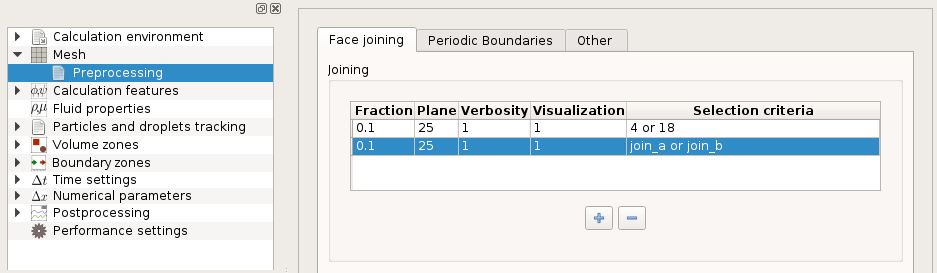
\includegraphics[width=0.9\textwidth]{gui_mesh_join}
\caption{Conformal or non-conformal joining}
\label{fig:joining}
\end{center}
\end{figure}
%
For a simple mesh, it is rarely useful to specify strict face selection
criteria, as joining is sufficiently automated to detect which faces
may actually be joined. For a more complex mesh, or a mesh with thin
walls which we want to avoid transforming into interior faces, it is
recommended to filter boundary faces that may be joined by using
face selection criteria. This has the
additional advantage of reducing the number of faces to test for
in the intersection/overlap search, and thus reduced to the time
required by the joining algorithm.

One may also modify tolerance criteria using 2 options:

\noindent
\begin{tabular}[top]{p{3.0cm}%
                     >{\PreserveBackslash\raggedright\hspace{0pt}}p{12.0cm}}
\texttt{fraction} $r$  &
assigns value $r$ (where $0 < r < 0.49$) to the maximum
intersection distance multiplier ($0.1$ by default). The maximum
intersection distance for a given vertex is based on the length of
the shortest incident edge, multiplied by $r$. The maximum intersection
at a given point along an edge is interpolated from that at its
vertices, as shown on the left of \figurename~\ref{fig:join_tolerance}; \\
\texttt{plane} $c$ &
assigns the maximum angle between normals for two faces to be
considered coplanar ($25^{\circ}$ by default);
this parameter is used in the second stage of the algorithm, to
reconstruct conforming faces, as shown on the right of figure
\ref{fig:join_tolerance}.\\
\end{tabular}

\begin{figure}[!hp]
\centerline{
\includegraphics*[width=14cm]{join_tolerance}}
\caption{Maximum intersection tolerance and faces normal angle
\label{fig:join_tolerance}}
\end{figure}

In practice, we are sometimes led to increase the maximum intersection
distance multiplier to $0.2$ or even $0.3$ when joining curved surfaces,
so that all intersection are detected. As this influences merging
of vertices and thus simplification of reconstructed faces, but also
deformation of ``lateral'' faces, it is recommended only to modify it
if necessary. As for the \texttt{plane} parameter, its use has
only been necessary on a few meshes up to now, and always in the
sense of reducing the tolerance so that face reconstruction does not
try to generate faces from initial faces on different surfaces.

\subsubsection{Periodicity\label{sec:optpcs:period}}

Handling of periodicity is based on an extension of conforming joining,
as shown on \figurename~\ref{fig:join_periodic}. It is thus not necessary
for the periodic faces to be conforming (though it usually leads to better
mesh quality). All options relative to conforming joining of
non-conforming faces also apply to periodicity. Note also that
once pre-processed, 2 periodic faces have the same orientation
(possibly adjusted by periodicity of rotation).

This operation can also be performed by the solver and specified
either using the GUI or the \\\texttt{cs\_user\_periodicity} function.

\begin{figure}[!hp]
\centerline{
\includegraphics*[height=8cm]{join_periodic}}
\caption{Matching of periodic faces
\label{fig:join_periodic}}
\end{figure}

As with joining, it is recommended to filter boundary faces to process
using a selection criterion. As many periodicities may be built as desired,
as long as boundary faces are present. Once a periodicity is handled,
faces having periodic matches do not appear as boundary faces, but as
interior faces, and are thus not available anymore for other
periodicities.

%==================================
\subsubsection{Parameters for conforming or non-conforming mesh joinings}
%==================================

The setting of these parameters is done in the user subroutine \texttt{cs\_user\_join} (called once). The user can specify the parameters used for the joining of different meshes. Below is given the list of the standard parameters which can me modified:
\begin{list}{-}{}
\item \texttt{fract}: the initial tolerance radius associated to each vertex is equal to the length of the shortest incident edge, multiplied by this fraction,
\item \texttt{plane}: when subdividing faces, 2 faces are considered coplanar and may be joined if the angle between their unit normals (in degrees) does not exceed this parameter,
\item \texttt{iwarnj}: the associated verbosity level (debug level if over 3).
\end{list}
In the call of the function \texttt{cs\_join\_add}, a selection criteria for
mesh faces to be joined is specified.

The call to the function '\texttt{cs\_join\_set\_advanced\_param}' allows defining parameters not available through the GUI.

The list of advanced modifiable parameters is given below:
\begin{list}{-}{}
\item \texttt{mtf}: a merge tolerance factor, used to locally modify the tolerance associated to each vertex before the merge step. Depending on its value, four
scenarios are possible:
\begin{list}{$\rightarrow$}{}
\item if $mtf=0$, no vertex merge
\item if $mtf<1$, the vertex merge is more strict. It may increase the number of tolerance reduction and therefore define smaller subset of vertices to merge together but it can drive to loose intersections.
\item if $mtf=1$, no change occurs
\item if $mtf>1$, the vertex merge is less strict. The subset of vertices able to merge is greater.
\end{list}
\item \texttt{pmf}: a pre-merge factor. This parameter is used to define a limit under which two vertices are merged before the merge step,
\item \texttt{tcm}: a tolerance computation mode. If its value is:
\begin{list}{$\rightarrow$}{}
\item 1 (default), the tolerance is the minimal edge length related to a vertex, multiplied by a fraction.
\item 2, the tolerance is computed like for 1 with, in addition, the multiplication by a coefficient equal to the maximum between $sin(e1)$ and $sin(e2)$; where $e1$ and $e2$ are two edges sharing the same vertex V for which we want to compute the tolerance.
\item 11, it is the same as 1 but taking into account only the selected faces.
\item 12, it is the same as 2 but taking into account only the selected faces.
\end{list}
\item \texttt{icm}: the intersection computation mode. If its value is:
\begin{list}{$\rightarrow$}{}
\item 1 (default), the original algorithm is used. Care should be taken to clip the intersection on an extremity.
\item 2, a new intersection algorithm is used. Caution should be used to avoid clipping the intersection on an extremity.
\end{list}
\item \texttt{maxbrk}: defines the maximum number of equivalence breaks which is enabled during the merge step,
\item \texttt{maxsf}: defines the maximum number of sub-faces used when splitting a selected face
\end{list}
%
The following are advanced parameters used in the search algorithm for face intersections between selected faces (octree structure). They are useful in case of memory limitation:
\begin{list}{-}{}
\item \texttt{tml}: the tree maximum level is the deepest level reachable during the tree building,
\item \texttt{tmb}: the tree maximum boxes is the maximum number of bounding boxes (BB) which can be linked to a leaf of the tree (not necessary true for the deepest level),
\item \texttt{tmr}: the tree maximum ratio. The building of the tree structure stops when the number of bounding boxes is superior to the product of \texttt{tmr} with the number of faces to locate. This is an efficient parameter to reduce memory consumption.
\end{list}

Examples of mesh modification are given in the following \doxygenfile{cs_user_mesh.html}{\texttt{doxygen} documentation}.

%==================================
\subsubsection{Parameters for periodicity}
%==================================

Periodicities can be set directly in the Graphical User Interface (GUI) or using the user function \texttt{cs\_user\_periodicity} (called once during the calculation initialisation). In both cases, the user can choose between 3 types of periodicities: translation, rotation, or mixed
(see \figurename\ref{fig:periodicities}).
Then specific parameters must be set.

\begin{figure}[!h]
\begin{center}
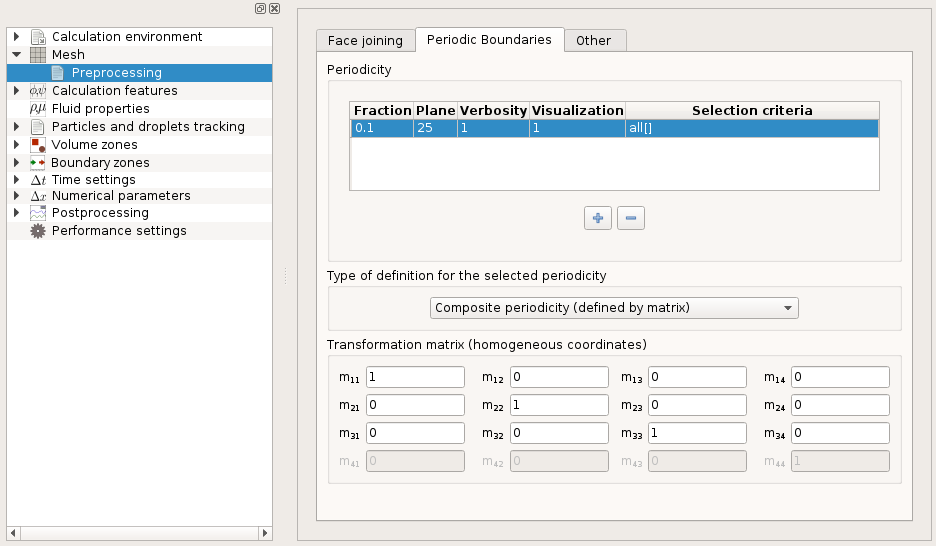
\includegraphics[width=0.9\textwidth]{gui_mesh_periodicity}
\caption{Periodicity}
\label{fig:periodicities}
\end{center}
\end{figure}

As periodicity is an extension of mesh joining, all parameters (whether basic or advanced) available for mesh joining are also applicable for periodicity, in addition to the parameters defining the periodicity transformation.

%==================================
\subsubsection{Modification of the mesh geometry}
%==================================
\noindent
\textit{Functions called only once during the calculation initialisation.}

The user function \texttt{cs\_user\_mesh\_input} allows a detailed
selection of imported meshes read, reading files multiple times,
applying geometric transformations, and renaming groups.

The user function \texttt{cs\_user\_mesh\_modify} may be used
for advanced modification of the main \texttt{cs\_mesh\_t}} structure.

{\em WARNING: Caution must be exercised when using this function
along with periodicity. Indeed, the periodicity parameters are not
updated accordingly, meaning that the periodicity may not be valid
after mesh vertex coordinates have changed. It is particularly
true when one rescales the mesh. Rescaling should thus be done
in a separate run, before defining periodicity.}

The user function \texttt{cs\_user\_mesh\_thinwall} allows
insertion of thin walls in the calculation mesh. Currently, this
function simply transforms the selected internal faces into boundary
faces, on which boundary conditions can (and must) be applied.

Faces on each side of a thin wall will share the same vertices,
so post-processing of the main volume mesh may not show the
inserted walls, though they will appear in the main boundary
output mesh.

%==================================
\subsection{Mesh smoothing utilities}
%==================================
\noindent
\textit{Function called once only during the calculation initialisation.}

The smoothing utilities may be useful when the calculation mesh has local
defects.
The principle of smoothers is to mitigate the local defects by averaging
the mesh quality. This procedure can help for calculation robustness or/and
results quality.

The user function \texttt{cs\_user\_mesh\_smoothe} allows to use different
smoothing functions detailed below.

{\em WARNING 1: Caution must be exercised when using this function
along with periodicity. Indeed, the periodicity parameters are not
currently updated accordingly, meaning that the periodicity may be
unadapted after one changes the mesh vertex coordinates. It is particularly
true when one rescales the mesh. Rescaling should thus be done
in a separate run, before defining periodicity.}

{\em WARNING 2: Caution must be exercised when using smoothing utilities
because the geometry may be modified. In order to preserve geometry,
the function} \texttt{cs\_mesh\_smoother\_fix\_by\_feature} {\em allows to
fix by a feature angle criterion the mobility of boundary vertices.}

\subsubsection{Fix by feature}
The vertex normals are defined by the average of the normals of the
faces sharing the vertex.
The feature angle between a vertex and one of its adjacent faces is defined
by the angle between the vertex normal and the face normal.

This function sets a vertex if one of its feature angles is less than
$cos(\theta)$ where $\theta$ is the maximum feature angle (in degrees)
defined by the user.
In fact, if $\theta = 0^{\circ}$ all boundary vertices will be fixed, and
if $\theta = 90^{\circ}$ all boundary vertices will be free.

Fixing all boundary vertices ensures the geometry is preserved, but reduces
the smoothing algorithm's effectiveness.

\subsubsection{Warped faces smoother}

The function \texttt{cs\_mesh\_smoother\_unwarp} allows reducing face warping
in the calculation mesh.

Be aware that, in some cases, this algorithm may degrade other mesh quality
criteria.

%==================================
\section{Partitioning for parallel runs\label{sec:parall:part}}
%==================================

Graph partitioning (using one of the optional \metis or
\scotch libraries) is done by the Solver. Unless explicitly
deactivated, this stage produces one or several ``cell $\rightarrow$ domain''
distribution files, named {\tt domain\_number\_\it{p}} for a partitioning on
$p$ sub-domains, which may be read when starting a subsequent computation so as
to avoid re-running that stage. These files are placed in a directory named
{\tt partition\_output}.

The Solver redistributes data read in {\tt mesh\_input} based on the associated
(re-read or computed) partitioning, so there is no need to run any
prior script when running on a different number of processors, although
a previous partitioning may optionally be re-used.

Without a graph-based partitioning library, or based on the user's choice,
the Solver will use a built-in partitioning using a space-filling curve
(Z or Hilbert curve) technique. This usually leads to partitionings
of lower quality than with graph partitioning, but parallel
performance remains reasonable.

Partitioning options may be defined using the GUI or by calling
the appropriate functions in the
\texttt{cs\_user\_partition\_options} user function.

\subsection{Partitioning stages\label{sec:parall:part:stages}}

Partitioning is always done just after reading the mesh, unless a
partitioning input file is available, in which case the partitioning
replaces this stage.

When a mesh modification implying a change of cell connectivity graph
is expected, the mesh may be repartitioned after the pre-processing
stage, prior to calculation. By default, re-partitioning is only done
if the partitioning algorithm chosen for that stage is expected to
produce different results due to the connectivity change. This is
the case for graph-based algorithms such as those of \metis or \scotch,
when mesh joining is defined, or additional periodic matching is defined
(and the algorithm is not configured to ignore periodicity information).

There are thus two possible partitioning stages:

\begin{itemize}
\item \texttt{CS\_PARTITION\_FOR\_PREPROCESS}, which is optional, and
      occurs just  after reading the mesh.
\item \texttt{CS\_PARTITION\_MAIN}, which occurs just after reading the
      mesh if it is the only stage, or after mesh preprocessing (and
      before computation), if the partitioning for preprocessing stage
      is activated.
\end{itemize}

The number of partitioning stages is determined automatically based on
information provided through \texttt{cs\_partition\_set\_preprocess\_hints()},
but repartitioning may also be forced or inhibited using the
\texttt{cs\_partition\_set\_preprocess()} user function.

\subsection{Partitioner choice\label{sec:parall:part:partlib}}

If the Solver has been configured with both \ptscotch or \scotch and
\parmetis or \metis libraries, \ptscotch will be used by default\footnote{
Though \parmetis will be chosen before serial \scotch in a parallel
run}, but the user may force the selection of another partitioning
type using either the GUI or user routines.

In addition to graph-based partitionings, a space-filling curve based
algorithm is available, using either a Morton (Z) or Peano-Hilbert
curve, in the computation domain's bounding box or bounding curve.

When partitioning for preprocessing, a space-filling curve is used,
unless forced by calling\\ \texttt{cs\_partition\_set\_algorithm()}
with the appropriate algorithm choice for the\\
\texttt{CS\_PARTITION\_FOR\_PREPROCESS} stage.

\subsection{Effect of periodicity\label{sec:parall:part:noperiod}}

By default, face periodicity relations are taken into account when building
the ``cell $\rightarrow$ cell'' connectivity graph used for partitioning.
This allows better partitioning optimization, but increases the probability
of having groups of cells at opposite sides of the domain in a same
sub-domain. This is not an issue for standard calculations, but may
degrade performance of search algorithms based on bounding boxes.
It is thus possible to ignore periodicity when partitioning a mesh.

Also, partitioning using a space-filling curve ignores periodicity.

Note that nothing guarantees that a graph partitioner will not place
disjoint cells in the same sub-domain independently of this option,
but this behaviour is rare.

%==================================
\section{Basic modelling setup}
%==================================

%==================================
\subsection{Initialisation of the main parameters}
%==================================

This operation is done in the Graphical User Interface (GUI) or by using the user subroutines in \\ \texttt{cs\_user\_parameters.f90}.
In the GUI, the initialisation is performed by filling the parameters displayed in \figurename\ref{fig:gui_calculation_features}
to \ref{fig:gui_output_profiles}. If the 'Mobile mesh' option is activated,
please see Section \ref{sec:ALE} for more details. The headings filled for the initialisation of the main parameters
are the followings:
\begin{list}{-}{}
\item Thermophysical model options: Steady or unsteady algorithm, specific physics, ALE mobile mesh,
      turbulence model, thermal model and species transport (definition of the scalars and their variances),
see \figurename~\ref{fig:gui_calculation_features} to \figurename~\ref{fig:gui_species}. If a thermal scalar, temperature or enthalpy, is selected,
two other headings on conjugate heat transfer and radiative transfers can be filled in (see \figurename~\ref{fig:gui_thermal_scalar}).
\item Body forces: gravity and coriolis forces, see \figurename~\ref{fig:gui_body_forces}.
\item Physical properties: reference pressure, velocity and length, fluid properties (density, viscosity, thermal conductivity,
specific heat and scalar diffusivity), see \figurename~\ref{fig:gui_reference_values} to \figurename~\ref{fig:gui_fluid_props}.
If non-constant values are used for the fluid properties, and if the GUI is not used, the \\ \texttt{cs\_user\_physical\_properties}
file must be used, see \S~\ref{sec:usphyv}.
\item Volume conditions: definition of volume regions (for initialisation, head losses and source terms,
see \S~\ref{sec:prg_usersourceterms} and \S~\ref{sec:prg_headlosses}), initialisation of the variables (including scalars), see \figurename~\ref{fig:gui_initialisation}.
\item Boundary conditions: definition and parametrisation of boundary conditions for all variables (including scalars).
If the GUI is not used, the \texttt{cs\_user\_boundary\_conditions} file must be used, see \S~\ref{sec:prg_boundaryconditions}.
\item Numerical parameters: number and type of time steps, and advanced parameters for the numerical solution of the equations,
see \figurename~\ref{fig:gui_global_parameters} to \figurename~\ref{fig:gui_time_step}.
\item Calculation control: parameters related to the time averages, the
      locations of the probes where some variables will be monitored over time
      (if the GUI is not used, this information is specified in \S~\ref{sec:cs_user_initialization}),
       the definition of the frequency of the outputs in the calculation
      log, the post-processing output writer frequency and format options, and
      the post-processing output meshes and variables selection, see
      \figurename~\ref{fig:gui_time_averages}, \figurename~\ref{fig:gui_output_log}, \figurename~\ref{fig:gui_output_writers},
      and \figurename~\ref{fig:gui_output_meshes}. The item ``Profiles'' allows to save, with a
      frequency defined by the user, 1D profiles on a parametric curve define by its equation, see \figurename\ref{fig:gui_output_profiles}.
\end{list}

\begin{figure}[!ht]
\begin{center}
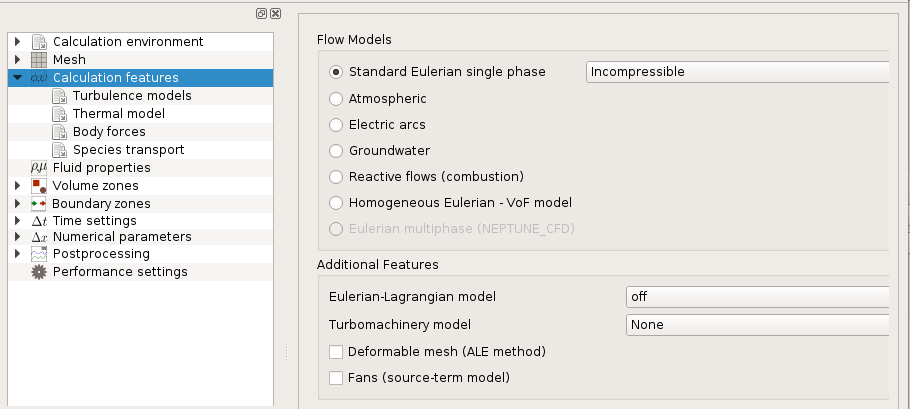
\includegraphics[width=0.9\textwidth]{gui_calculation_features}
\caption{Calculation features options}
\label{fig:gui_calculation_features}
\end{center}
\end{figure}

\begin{figure}[!ht]
\begin{center}
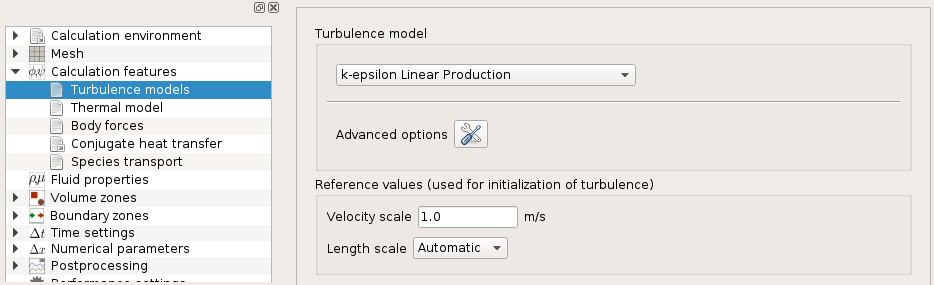
\includegraphics[width=0.9\textwidth]{gui_turbulence_models}
\caption{Turbulence model selection}
\label{fig:gui_turbulence_models}
\end{center}
\end{figure}

\begin{figure}[!ht]
\begin{center}
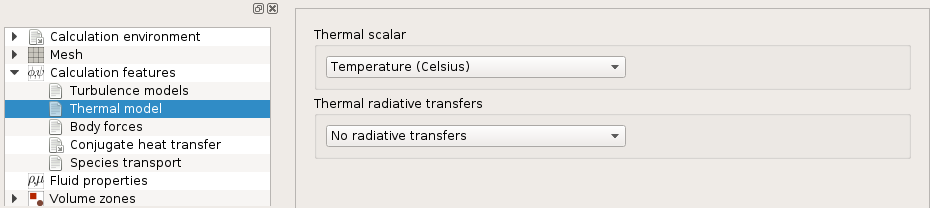
\includegraphics[width=0.9\textwidth]{gui_thermal_scalar}
\caption{Thermal scalar selection}
\label{fig:gui_thermal_scalar}
\end{center}
\end{figure}

\begin{figure}[!ht]
\begin{center}
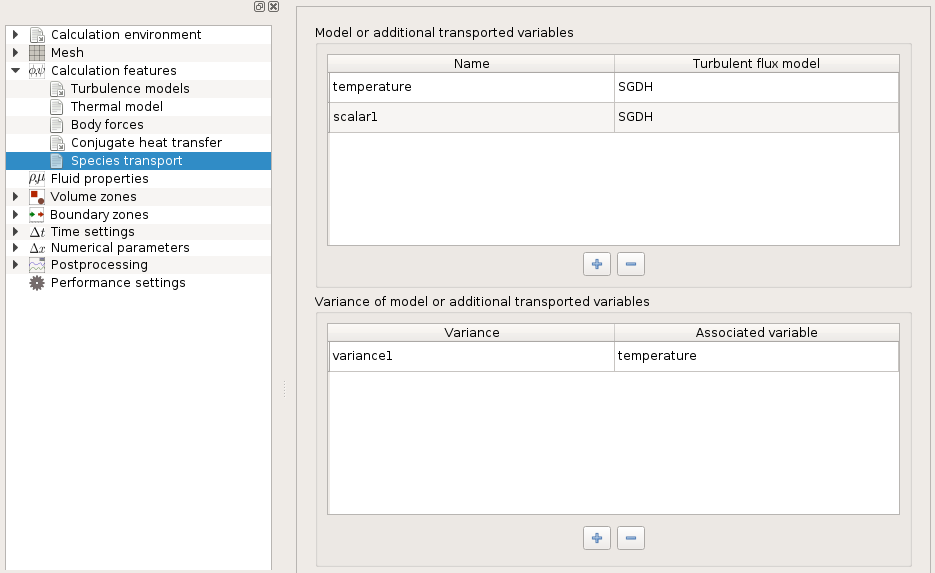
\includegraphics[width=\textwidth]{gui_user_scal_def_init}
\caption{Definition of the transported species/scalars}
\label{fig:gui_species}
\end{center}
\end{figure}

\begin{figure}[!ht]
\begin{center}
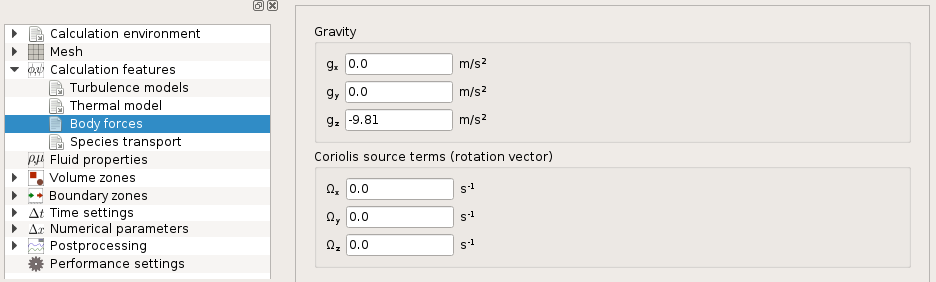
\includegraphics[width=0.9\textwidth]{gui_body_forces}
\caption{Setting of the gravity}
\label{fig:gui_body_forces}
\end{center}
\end{figure}

\begin{figure}[!ht]
\begin{center}
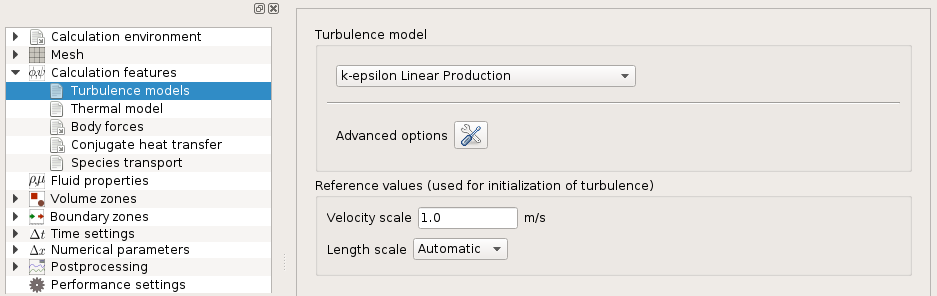
\includegraphics[width=13cm]{gui_phys_prop_reference_values}
\caption{Setting of the reference values for pressure, velocity and length}
\label{fig:gui_reference_values}
\end{center}
\end{figure}

\begin{figure}[!ht]
\begin{center}
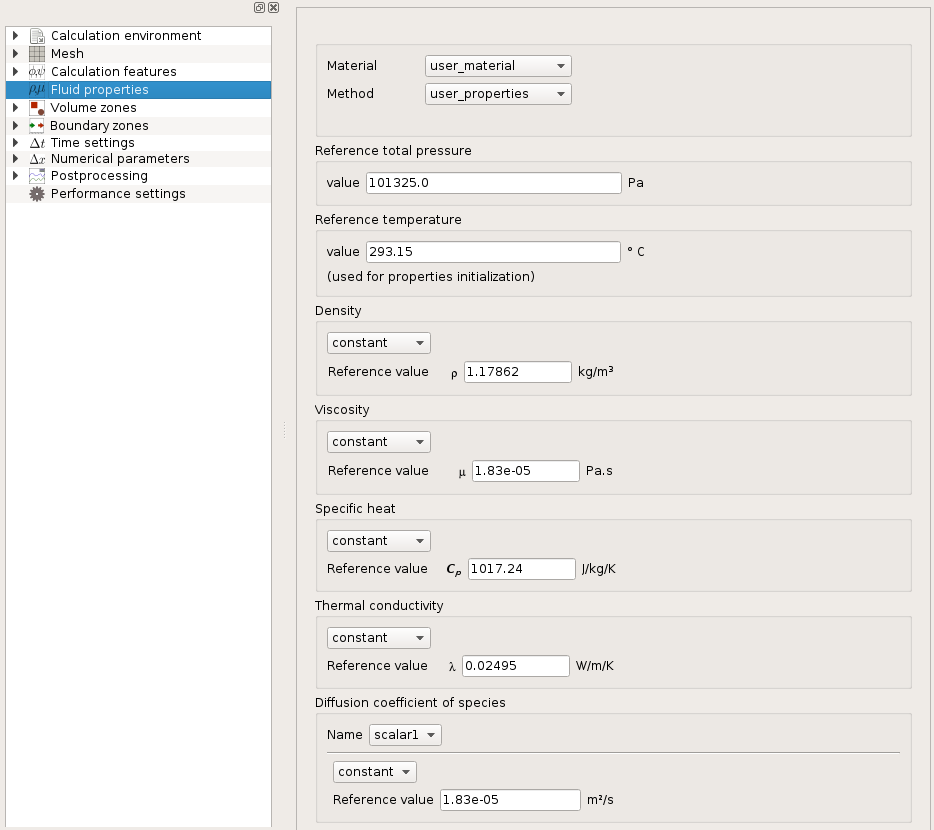
\includegraphics[width=\textwidth]{gui_fluid_props}
\caption{Fluid properties}
\label{fig:gui_fluid_props}
\end{center}
\end{figure}

\begin{figure}[!ht]
\begin{center}
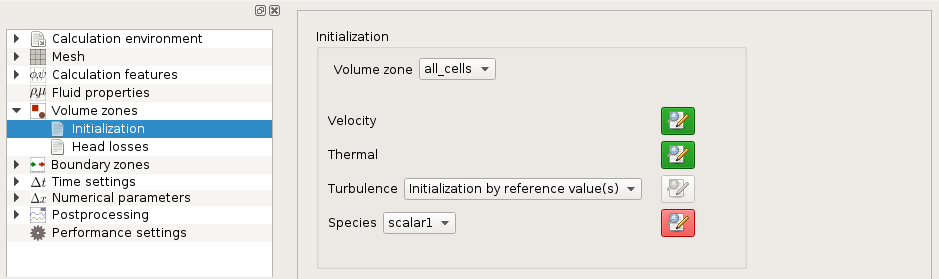
\includegraphics[width=\textwidth]{gui_initialisation}
\caption{Initialisation of variables}
\label{fig:gui_initialisation}
\end{center}
\end{figure}

\begin{figure}[!ht]
\begin{center}
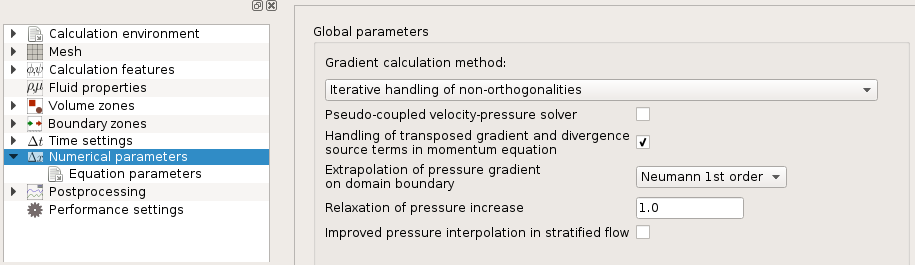
\includegraphics[width=\textwidth]{gui_global_res_parameters}
\caption{Global resolution parameters}
\label{fig:gui_global_parameters}
\end{center}
\end{figure}

\begin{figure}[!ht]
\begin{center}
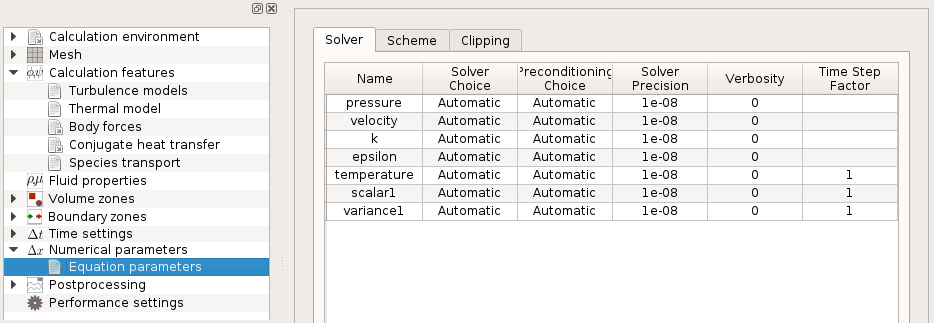
\includegraphics[width=0.9\textwidth]{gui_numerical_parameters}
\caption{Numerical parameters for the main variables resolution}
\label{fig:gui_numerical_parameters}
\end{center}
\end{figure}

\begin{figure}[!ht]
\begin{center}
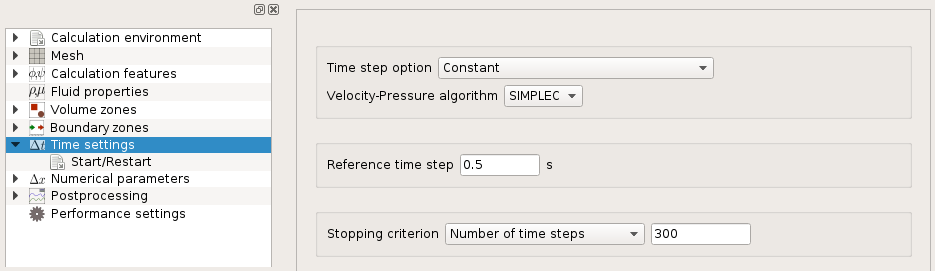
\includegraphics[width=0.9\textwidth]{gui_time_step}
\caption{Time step settings}
\label{fig:gui_time_step}
\end{center}
\end{figure}

\begin{figure}[!ht]
\begin{center}
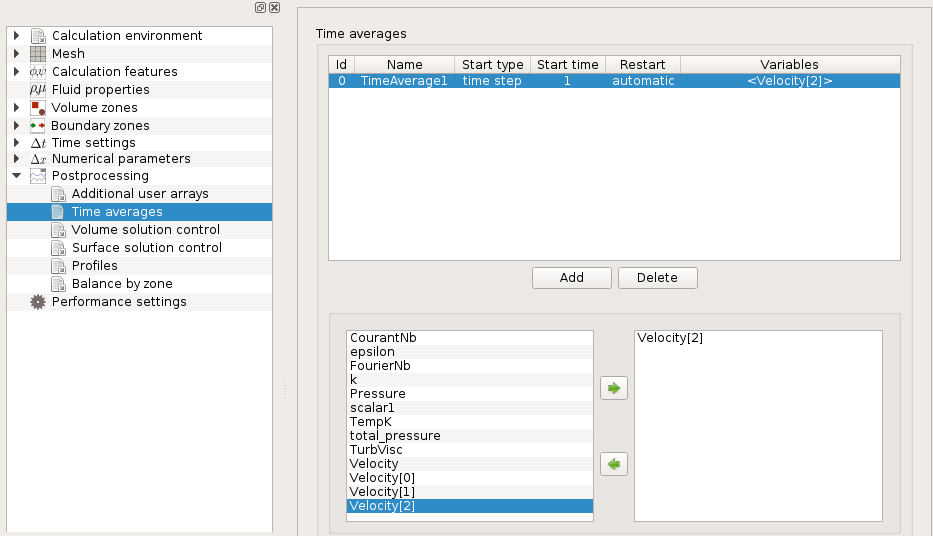
\includegraphics[width=0.9\textwidth]{gui_time_averages}
\caption{Management of time averaged variables}
\label{fig:gui_time_averages}
\end{center}
\end{figure}

\begin{figure}[!ht]
\begin{center}
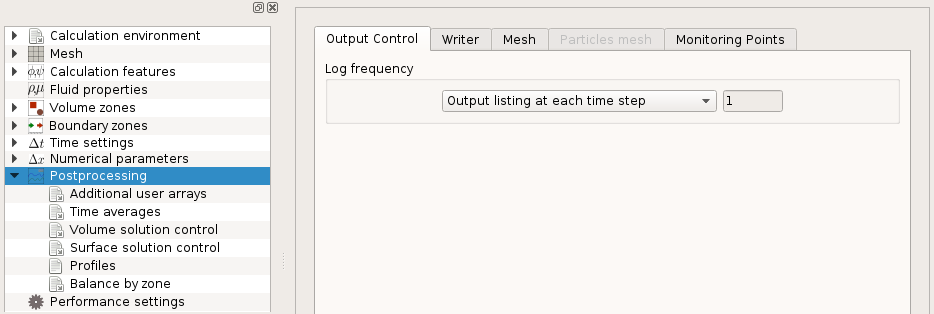
\includegraphics[width=0.9\textwidth]{gui_output_log}
\caption{Parameters of chronological logging options}
\label{fig:gui_output_log}
\end{center}
\end{figure}

\begin{figure}[!ht]
\begin{center}
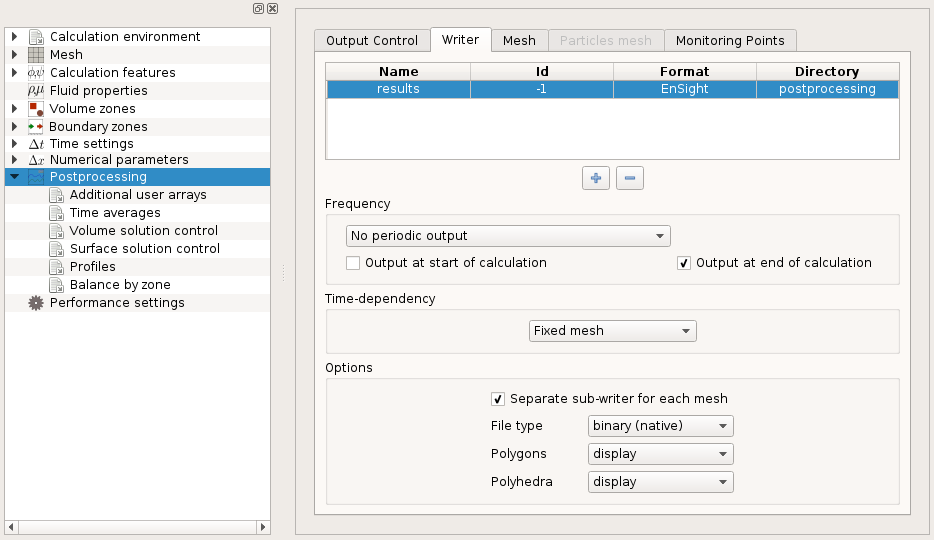
\includegraphics[width=0.9\textwidth]{gui_output_writers}
\caption{Management of postprocessing writers}
\label{fig:gui_output_writers}
\end{center}
\end{figure}

\begin{figure}[!ht]
\begin{center}
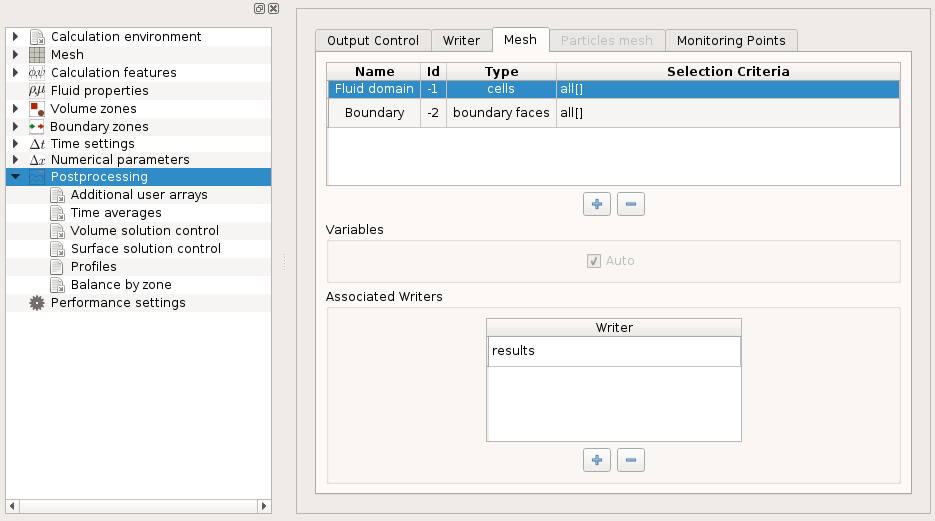
\includegraphics[width=0.9\textwidth]{gui_output_meshes}
\caption{Management of postprocessing meshes}
\label{fig:gui_output_meshes}
\end{center}
\end{figure}

\begin{figure}[!ht]
\begin{center}
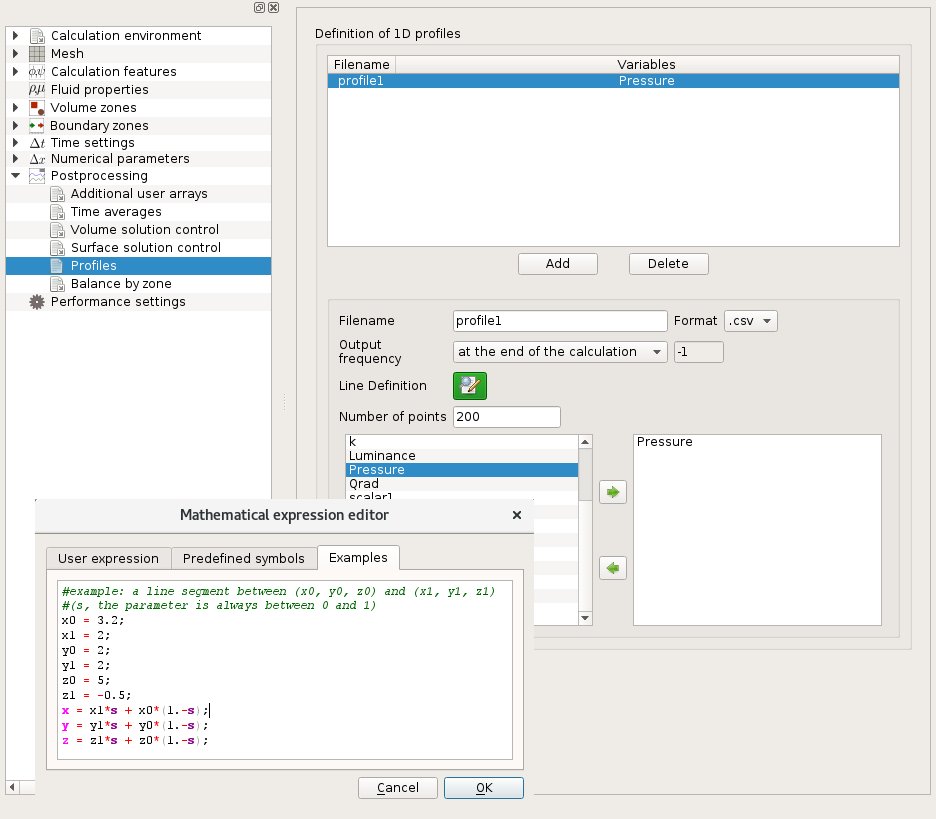
\includegraphics[width=0.9\textwidth]{gui_output_profiles}
\caption{Management of 1D profiles of the solution}
\label{fig:gui_output_profiles}
\end{center}
\end{figure}

With the GUI, the subroutine \texttt{cs\_user\_parameters.f90} is only
used to modify high-level parameters which can not be managed by the
interface. Without the GUI, this
subroutine is compulsory and some of the headings must be completed (see \S\ref{sec:prg_stepbystepcalculation}).
\texttt{cs\_user\_parameters.f90}
is used to indicate the value of different calculation
basic parameters: constant and uniform physical values, parameters of
numerical schemes, input-output management...\\
It is called only during the calculation initialisation.

For more details about the different parameters, please refer to the key
word list (\S\ref{sec:prg_motscles}).

\texttt{cs\_user\_parameters.f90} is in fact constituted of 4 separate subroutines:  \texttt{usipph}, \texttt{usppmo},
\texttt{usipsu} and \texttt{usipes}. Each one controls various
 specific parameters. The keywords which are not featured in the supplied example
can be provided by the user in \texttt{SRC/REFERENCE/base}; in this case,
understanding of the comments is required to add the keywords in the appropriate
subroutine, it will ensure that the value
has been well defined. The modifiable parameters in each of the subroutines of
\texttt{cs\_user\_parameters.f90} are:

\begin{list}{$\bullet$}{}
\item \texttt{usipph}: \texttt{iturb}, \texttt{itherm} and \texttt{icavit} (don't modify these
      parameters anywhere else)
\item \texttt{usppmo}: activation of specific physical models.
\item \texttt{usipsu}: physical parameters of the calculation (thermal scalar, physical
      properties, ...), numerical parameters (time steps, number of iterations, ...),
      definition of the time averages.
\item \texttt{usipes}: post-processing output parameters (periodicity, variable names,
      probe positions, ...)
\end{list}

For more details on the different parameters, see the list of keywords
(\S~\ref{sec:prg_motscles}).
 The names of the keywords can also be seen in the help sections of the interface.

\noindent
$\bullet\ $ When using the interface, only the
additional parameters (which can not be defined in the interface)
should appear in \texttt{cs\_user\_parameters.f90}. The user
needs then only to activate examples which are useful for his
case (replacing \texttt{if (.false.)} with \texttt{if (.true.)},
or removing such tests).

\subsection{Selection of mesh inputs: \textmd{\texttt{cs\_user\_mesh\_input}}}
%==================================

\noindent
\textit{Subroutine called only during the calculation initialisation.}

This C function may be used to select which mesh input files
are read, and apply optional coordinate transformations or group renumberings
to them. By default, the input read is a file or directory named
\texttt{mesh\_input}, but if this function is used, any file can be selected,
and the same file can be read multiple times (applying a different
coordinate transformation each time).
All inputs read through this function are automatically concatenated, and
may be later joined using the mesh joining options.

Geometric transformations are defined using a homogeneous coordinates
transformation matrix. Such a matrix has 3 lines and 4 columns, with the
first 3 columns describing a rotation/scaling factor, and the last column
describing a translation. A 4th line is implicit, containing zeroes
off-diagonal, and 1 on the diagonal. The advantages of this representation
is that any rotation/translation/scaling combination may be expressed
by matrix multiplication, while simple rotations or translations
may still be defined easily.

%==================================
%==================================
\subsection{Non-default variables initialisation} \label{sec:cs_user_initialization}
%==================================

The non-default variables initialisation is performed in the subroutine \texttt{cs\_user\_initialization} (called only during the calculation initialisation).\\ At the calculation beginning, the variables are initialised
automatically by the code. Velocities and scalars are set to 0 (or \texttt{scamax} or \texttt{scamin} if 0 is outside the acceptable
scalar variation range), and the turbulent variables are estimated from
\texttt{uref} and \texttt{almax}. \\
For $k$ (of variable index \texttt{ik}) in the $k-\varepsilon$,
$R_{ij}-\varepsilon$, v2f or $k-\omega$ models:
\begin{equation*}
k = 1.5 \left(0.02 \textrm{ \texttt{uref}}\right)^2
\end{equation*}
and in $R_{ij}-\varepsilon$:
\begin{equation*}
R_{ij}=\frac{2}{3}k\delta_{ij}
\end{equation*}
For $\varepsilon$ (of variable index \texttt{iep}) in the $k-\varepsilon$,
$R_{ij}-\varepsilon$ or v2f models:
\begin{equation*}
\varepsilon = k^{1.5} \frac{C_\mu}{\textrm{\texttt{almax}}}
\end{equation*}
For $\omega$ (of variable index \texttt{iomg}) in the $k-\omega$ model:
\begin{equation*}
\omega = k^{0.5} \frac{1}{\textrm{\texttt{almax}}}
\end{equation*}
For $\varphi$ and $\overline{f}$ (of variable indices \texttt{iphi} and
\texttt{ifb}) in the v2f models:
\begin{equation*}
\left\{\begin{array}{ll}
\varphi = & \frac{2}{3} \\
\overline{f} = & 0
\end{array}\right.
\end{equation*}
For $\alpha$ (of variable index \texttt{ial}) in the EBRSM and BL-v2/k models:
\begin{equation*}
\alpha = 1
\end{equation*}
For $\tilde{\nu}_t$ in the Spalart-Allmaras model:
\begin{equation*}
\tilde{\nu}_t = 0.02 \sqrt{\frac{3}{2}} (\textrm{\texttt{uref}}) (\textrm{\texttt{almax}})
\end{equation*}

The subroutine \texttt{cs\_user\_initialization} allows if necessary to
initialise certain variables to values closer to their estimated final values,
in order to obtain a faster convergence.

This subroutine allows also the user to make a non-standard initialisation of
physical parameters (density, viscosity, ...), to impose a local
value of the time step, or to modify some parameters (time step,
variable specific heat, ...) in the case of a calculation restart.

\minititre{Note: value of the time step}
\begin{list}{-}{}
\item For calculations with constant and uniform time step
      (\texttt{idtvar}=0), the value of the time step is \texttt{dtref},
      given in the parametric file of the interface or in
      \texttt{cs\_user\_parameters.f90}.
\item For calculations with a non-constant time step
      (\texttt{idtvar}=1 or 2), which is not a calculation restart,
      the value of \texttt{dtref} given in the parametric file of the interface
      or in \texttt{cs\_user\_parameters.f90} is used to initialise the time
      step.
\item For calculations with a non-constant time step
      (\texttt{idtvar}=1 or 2) which is a restart of a
      calculation whose time step type was different (for instance, restart
      using a variable time step of a calculation run using a constant time
      step), the value of \texttt{dtref}, given in the parametric file of the
      interface or in \texttt{cs\_user\_parameters.f90}, is used to initialise
      the time step.
\item For calculations with non-constant time step
      (\texttt{idtvar}=1 or 2) which is a restart of a
      calculation whose time step type was the same (for instance, restart with
      \texttt{idtvar}=1 of a calculation run with \texttt{idtvar}=1), the time
      step is read from the restart file and the value of \texttt{dtref} given
      in the parametric file of the interface, or in
      \texttt{cs\_user\_parameters.f90}, is not used.
\end{list}
It follows, that for a calculation with a non-constant time step
(\texttt{idtvar}=1 or 2) which is a restart of a calculation in which
\texttt{idtvar} had the same value, \texttt{dtref} does not allow to modify the
time step. The user subroutine \texttt{cs\_user\_initialization} allows
modifying the array \texttt{dt} which contains the value of the time step read
from the restart file (array whose size is \texttt{ncelet}, defined at the cell
centres whatever the chosen time step type is).

\clearpage

%==================================
\subsection{Manage boundary conditions}
%==================================
\label{sec:prg_boundaryconditions}
The boundary conditions can be specified in the Graphical User Interface (GUI) under the heading ``Boundary conditions''
or in the user subroutine \texttt{cs\_user\_boundary\_conditions} called every time step.
With the GUI, each region and the type of boundary condition associated to it are defined in
\figurename~\ref{fig:gui_bc_regions}. Then, the parameters of the boundary condition are specified
 in \figurename~\ref{fig:gui_bc_parameters}. The colors of the boundary faces may be read directly from
a ``preprocessor.log'' file created by the Preprocessor. This file can be generated directly by the interface
under the heading ``Definition of boundary regions $\rightarrow$ Add from Preprocessor log $\rightarrow$ import groups and references from Preprocessor log'', see \figurename~\ref{fig:gui_bc_regions}.
%
\begin{figure}[!ht]
\begin{center}
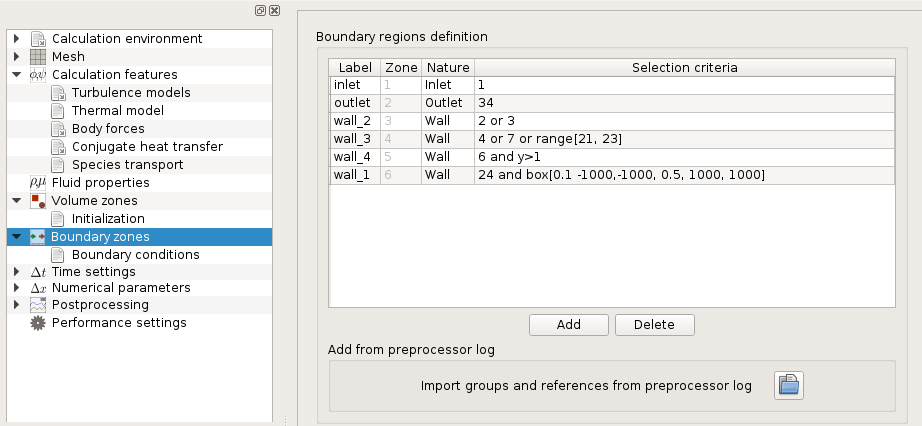
\includegraphics[width=0.9\textwidth]{gui_bc_regions}
\caption{Definition of the boundary conditions}
\label{fig:gui_bc_regions}
\end{center}
\end{figure}
%
\begin{figure}[!ht]
\begin{center}
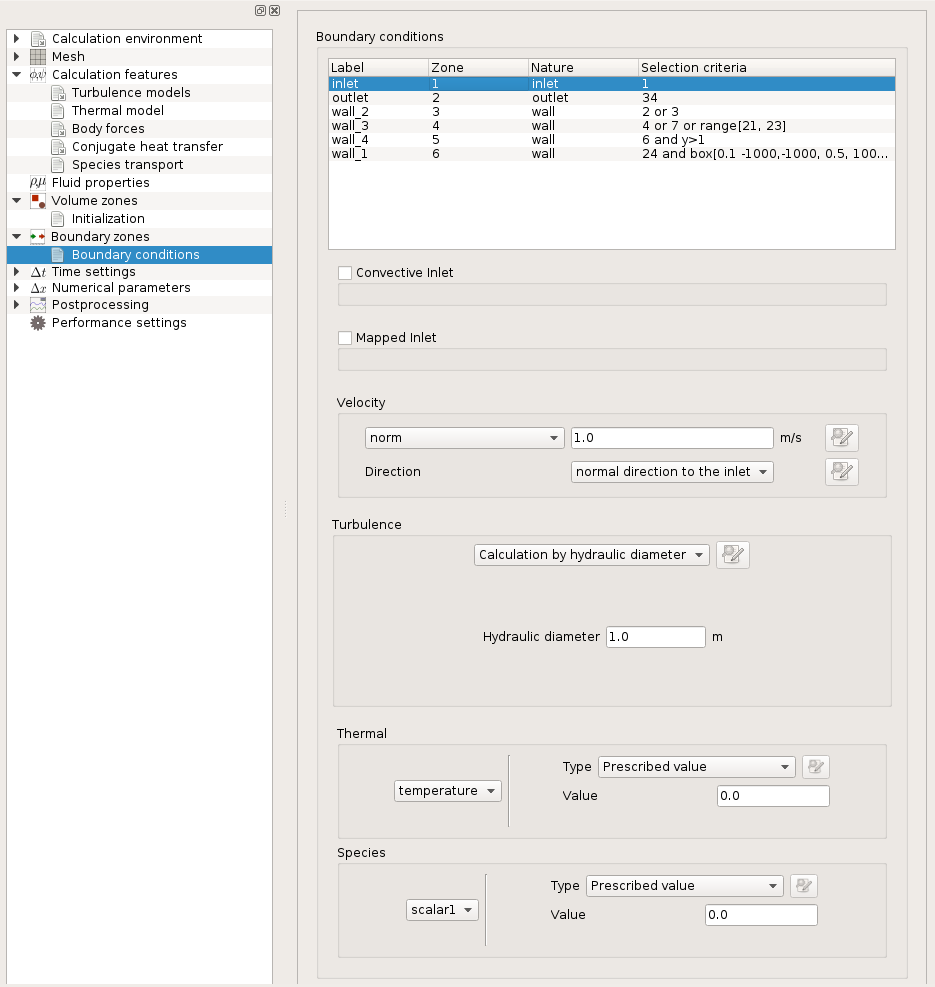
\includegraphics[width=13cm]{gui_bc_parameters}
\caption{Parameters of the boundary conditions}
\label{fig:gui_bc_parameters}
\end{center}
\end{figure}
%
\texttt{cs\_user\_boundary\_conditions} is the second compulsory subroutine for every calculation launched
without interface (except in the case of specific physics where the
corresponding boundary condition user subroutine must be used).

When using the interface, only complex boundary conditions (input profiles, conditions varying in time, ...)
need to be defined with \texttt{cs\_user\_boundary\_conditions}.
In the case of a calculation launched without the
interface, all the boundary conditions must appear in \texttt{cs\_user\_boundary\_conditions}.

\texttt{cs\_user\_boundary\_conditions} is essentially constituted of loops on boundary
face subsets. Several sequences
of \verb+call getfbr+ \verb+('criterion', nlelt, lstelt)+ (cf.
\S\ref{sec:fvm_selector}) allow selecting
the boundary faces with respect to their group(s), their
color(s) or geometric criteria. If needed, geometric and
physical variables are also available to the user. These allow him
to select the boundary faces using other criteria.

For more details about the treatment of boundary conditions, the user
may refer to the theoretical and computer documentation \cite{theory} of
the subroutine \texttt{condli} (for wall conditions, see
\texttt{clptur}) (to access this document on a workstation, use
\mbox{\texttt{code\_saturne~info --guide theory}}).

From the user point of view, the boundary conditions are fully
defined by three arrays\footnote{Except with Lagrangian boundary condition}:
\texttt{itypfb(nfabor)}\index{\texttt{itypfb}},
\texttt{icodcl(nfabor,nvar)}\index{\texttt{icodcl}} and
\texttt{rcodcl(nfabor,nvar,3)}\index{\texttt{rcodcl}}.
\begin{list}{-}{}
\item \texttt{itypfb(ifac)} defines the type of the face \texttt{ifac}
      (input, wall, ...).
\item \texttt{icodcl(ifac,ivar)} defines the type of boundary
      condition for the variable \texttt{ivar} on the face \texttt{ifac}
      (Dirichlet, flux ...).
\item \texttt{rcodcl(ifac,ivar,.)} gives the numerical values associated with the
      type of boundary condition (value of the Dirichlet condition, of the flux ...).
\end{list}

In the case of standard boundary conditions (see
\S\ref{sec:prg_clstandard}), it is sufficient to complete \texttt{itypfb(ifac)} and
parts of the array \texttt{rcodcl}; the array \texttt{icodcl} and most of \texttt{rcodcl} are filled automatically. For non-standard boundary
conditions (see \S\ref{sec:prg_clnonstandard}), the arrays \texttt{icodcl} and
\texttt{rcodcl} must be fully completed.

%==================================
\subsubsection{Coding of standard boundary conditions}
%==================================
\label{sec:prg_clstandard}%
The standard keywords used by the indicator \texttt{itypfb} are:
\texttt{ientre\index{ientre}}, \texttt{iparoi\index{iparoi}},
\texttt{iparug\index{iparug}}, \texttt{isymet\index{isymet}},
\texttt{isolib\index{isolib}}, \texttt{ifrent\index{ifrent}}, \texttt{ifresf\index{ifresf}},
\texttt{i\_convective\_inlet\index{i\_convective\_inlet}} and \texttt{iindef\index{iindef}}.

\begin{list}{$\bullet$}{}
\item If \texttt{itypfb=ientre}: inlet face.

\begin{list}{$\rightarrow$}{}
\item Zero-flux condition for pressure and Dirichlet condition for all
      other variables. The value of the Dirichlet condition must be given in
      \texttt{rcodcl(ifac,ivar,1)} for every value of \texttt{ivar}, except for
      \texttt{ivar=ipr}. The other values of \texttt{rcodcl} and
      \texttt{icodcl} are filled automatically.
\end{list}

\item If \texttt{itypfb=iparoi}: smooth solid wall face, impermeable and with friction.

\begin{list}{$\rightarrow$}{}
\item the eventual sliding wall velocity of the face is
      found in \texttt{rcodcl(ifac,ivar,1)} (\texttt{ivar} being
      \texttt{iu}, \texttt{iv} or \texttt{iw}). The initial
      values of \texttt{rcodcl(ifac,ivar,1)} are zero for
      the three velocity components (and therefore are to be specified
      only if the velocity is not equal to zero). \\
{\em WARNING: the wall sliding velocity must belong to the boundary face
      plane. For safety, the code only uses the projection of this
      velocity on the face. As a consequence, if the velocity specified
      by the user does not belong to the face plane, the wall sliding velocity really
      taken into account will be different.}

\item For scalars, two kinds of boundary conditions can be
      defined:
\begin{list}{$\rightsquigarrow$}{}
\item Imposed value at the wall. The user must write\\
\hspace*{1cm}\texttt{icodcl(ifac,ivar)}=5\\
\hspace*{1cm}\texttt{rcodcl(ifac,ivar,1)}=imposed value\\
\item Imposed flux at the wall. The user must write\\
\hspace*{1cm}\texttt{icodcl(ifac,ivar)}=3\\
\hspace*{1cm}\texttt{rcodcl(ifac,ivar,3)}=imposed flux value (depending on the
variable, the user may refer to the case \texttt{icodcl}=3 of \S~\ref{sec:prg_clnonstandard} for the flux definition).
\item If the user does not fill these arrays, the default condition
      is zero flux.
\end{list}
\end{list}

\item If \texttt{itypfb=iparug}: rough solid wall face, impermeable and with friction.

\begin{list}{$\rightarrow$}{}
\item the eventual moving velocity of the wall tangent to the face is
      given by \texttt{rcodcl(ifac,ivar,1)} (\texttt{ivar} being
      \texttt{iu}, \texttt{iv} or \texttt{iw}). The initial
      value of \texttt{rcodcl(ifac,ivar,1)} is zero for
      the three velocity components (and therefore must be specified
      only in the case of the existence of a slipping velocity). \\
{\em WARNING: the wall moving velocity must be in the boundary face
      plane. By security, the code uses only the projection of this
      velocity on the face. As a consequence, if the velocity specified
      by the user is not in the face plane, the wall moving velocity really
      taken into account will be different.}
\item The dynamic roughness must be specified in \texttt{rcodcl(ifac,iu,3)}.
      The values of \texttt{rcodcl(ifac,iv,3)} stores the thermal and scalar roughness.
      The values of \texttt{rcodcl(ifac,iw,3)} is not used.
\item For scalars, two kinds of boundary conditions can be defined:
\begin{list}{$\rightsquigarrow$}{}
\item Imposed value at the wall. The user must write\\
\hspace*{1cm}\texttt{icodcl(ifac,ivar)}=6\\
\hspace*{1cm}\texttt{rcodcl(ifac,ivar,1)}=imposed value\\
\item Imposed flux at the wall. The user must write\\
\hspace*{1cm}\texttt{icodcl(ifac,ivar)}=3\\
\hspace*{1cm}\texttt{rcodcl(ifac,ivar,3)}= imposed flux value (definition
      of the flux condition according to the variable, the user can refer to the
      case \texttt{icodcl}=3 of the paragraph \ref{sec:prg_clnonstandard}).
\item If the user does not complete these arrays, the default condition
      is zero flux.
\end{list}
\end{list}
\item If \texttt{itypfb=isymet}: symmetry face (or wall without friction).
\begin{list}{$\rightarrow$}{}
\item Nothing to be writen in \texttt{icodcl} and  \texttt{rcodcl}.
\end{list}

\item If \texttt{itypfb=isolib}: free outlet face (or more precisely free
      inlet/outlet with forced pressure)
\begin{list}{$\rightarrow$}{}
\item The pressure is always treated with a Dirichlet condition, calculated
      with the constraint $\displaystyle \frac{\partial }{\partial n}\left(\frac{ \partial P}{\partial \tau}\right)=0$.
      The pressure is set to $P_0$ at the first \texttt{isolib} face met.
      The pressure calibration is always done on a single face, even if there are
      several outlets.
\item If the mass flow is coming in, the velocity is set to zero
      and a Dirichlet condition for the scalars and the turbulent quantities is used
      (or zero-flux condition if no Dirichlet value has been specified).
\item If the mass flow is going out, zero-flux condition are set for the velocity,
      the scalars and the turbulent quantities.
\item Nothing is written in \texttt{icodcl} or \texttt{rcodcl} for the pressure or
      the velocity. An optional Dirichlet condition can be specified for the scalars
      and turbulent quantities.
\end{list}

\item If \texttt{itypfb=ifrent}: free outlet, free inlet (based on Bernoulli relationship) face.

\begin{list}{$\rightarrow$}{}
\item if outlet, the equivalent to standard outlet.
      In case of ingoing flux, the Benoulli relationship which links pressure and velocity is used (see the thory guide for more information). An additional head loss modelling what is going on outward of the domain can be added by the user.
\end{list}

\item If \texttt{itypfb=ifresf}: free-surface boundary condition.

\item If \texttt{itypfb=i\_convective\_inlet}: inlet with zero diffusive flux for all transported variables (species and velocity). This allows to exactly impose the ingoing flux.

\item If \texttt{itypfb=iindef}: undefined type face (non-standard case).
\begin{list}{$\rightarrow$}{}
\item Coding is done in a non-standard way by filling both arrays \texttt{rcodcl} and
      \texttt{icodcl} (see \S~\ref{sec:prg_clnonstandard}).
\end{list}
\end{list}

\minititre{Notes}
$\bullet\ $ Whatever is the value of the indicator \texttt{itypfb(ifac)}, if
the array \texttt{icodcl(ifac,ivar)} is modified by the user ({\em i.e.} filled
with a non-zero value), the code will not use the default
conditions for the variable \texttt{ivar} at the face \texttt{ifac}. It will
take into account only the values of \texttt{icodcl} and \texttt{rcodcl} provided by the
user (these arrays must then be fully completed, like in the non-standard case). \\
For instance, for a normal symmetry face where scalar 1 is associated with a
Dirichlet condition equal to 23.8 (with an infinite exchange
coefficient):\\
\hspace*{2cm}\texttt{itypfb(ifac)=isymet}\\
\hspace*{2cm}\texttt{icodcl(ifac,isca(1))=1}\\
\hspace*{2cm}\texttt{rcodcl(ifac,isca(1),1)=23.8}\\
(\texttt{rcodcl(ifac,isca(1),2)=rinfin} is the default value, therefore it is
not necessary to specify a value)\\
The boundary conditions for the other variables are automatically
defined.

\noindent
$\bullet\ $The user can define new types of boundary faces. He only must
choose a value $N$ and to fully specify the boundary conditions (see
\S\ref{sec:prg_clnonstandard}). He must specify
\texttt{itypfb(ifac)}=$N$ where $N$ range is 1 to
\texttt{ntypmx\index{ntypmx}} (maximum number of boundary face types), and of
course different from the values \texttt{ientre}, \texttt{iparoi},
\texttt{iparug}, \texttt{isymet}, \texttt{isolib} and \texttt{iindef} (the values
of these variables are given in the \texttt{paramx} module). This allows to
easily isolate some boundary faces, in order for instance to calculate balances.

%==================================
\subsubsection{Coding of non-standard boundary conditions}
%==================================
\label{sec:prg_clnonstandard}%
Ifa face does not correspond to a standard type, the user
must completely fill the arrays \texttt{itypfb}, \texttt{icodcl} and
\texttt{rcodcl}. \texttt{itypfb(ifac)} is then equal to \texttt{iindef}
or another value defined by the user (see note at the end of
\S~\ref{sec:prg_clstandard}). The arrays \texttt{icodcl} and \texttt{rcodcl}
must be filled as follows:

\begin{list}{$\bullet$}{}
\item If \texttt{icodcl(ifac,ivar)}=1: Dirichlet condition at the face
      \texttt{ifac} for the variable \texttt{ivar}.

\begin{list}{$\rightarrow$}{}
\item \texttt{rcodcl(ifac,ivar,1)} is the value of the variable \texttt{ivar}
      at the face \texttt{ifac}.

\item \texttt{rcodcl(ifac,ivar,2)} is the value of the exchange coefficient
      between the outside and the fluid for the variable \texttt{ivar}. An
      infinite value (\texttt{rcodcl(ifac,ivar,2)=rinfin}) indicates an
      ideal transfer between the outside and the fluid (default case).

\item \texttt{rcodcl(ifac,ivar,3)} is not used.

\item \texttt{rcodcl(ifac,ivar,1)} has the units of the variable
      \texttt{ivar}, {\em i.e.}:
\begin{list}{$\rightsquigarrow$}{}
\item $m/s$ for the velocity

\item $m^2/s^2$ for the Reynolds stress

\item $m^2/s^3$ for the dissipation

\item $Pa$ for the pressure

\item \degresC\ for the temperature

\item $J.kg^{-1}$ for the enthalpy

\item \degresC$^2$ for temperature fluctuations

\item $J^2.kg^{-2}$ for enthalpy fluctuations
\end{list}

\item \texttt{rcodcl(ifac,ivar,2)} has the following units (defined in such way
      that when multiplying the exchange coefficient by the variable, the
      given flux has the same units as the flux defined below when
      \texttt{icodcl=3}):

\begin{list}{$\rightsquigarrow$}{}
\item $kg.m^{-2}.s^{-1}$ for the velocity

\item $kg.m^{-2}.s^{-1}$ for the Reynolds stress

\item $s.m^{-1}$ for the pressure

\item $W.m^{-2}.\mbox{\degresC}^{-1}$ for the temperature

\item $kg.m^{-2}.s^{-1}$ for the enthalpy
\end{list}

\end{list}

\item If \texttt{icodcl(ifac,ivar)=2}: radiative outlet at the face \texttt{ifac}
      for the variable \texttt{ivar}. It reads $ \dfrac{\partial \varia }{\partial t} + C \dfrac{\partial \varia}{\partial n} = 0 $, where $C$ is a to be defined celerity of radiation.

\begin{list}{$\rightarrow$}{}
\item \texttt{rcodcl(ifac,ivar,3)} is not used.

\item \texttt{rcodcl(ifac,ivar,1)} is the flux value of \texttt{ivar} at the cell center $\centip$,
      projection of the center of the adjacent cell on the straight line
      perpendicular to the boundary face and crossing its center,
      at the previous time step.
      It corresponds to:
\item \texttt{rcodcl(ifac,ivar,2)} is CFL number based on the parameter $C$,
      the distance to the boundary $\centip \centf$ and the time step:
      $CFL = \dfrac{C dt }{\centip \centf}$,

\end{list}

\item If \texttt{icodcl(ifac,ivar)=3}: flux condition at the face \texttt{ifac}
      for the variable \texttt{ivar}.

\begin{list}{$\rightarrow$}{}
\item \texttt{rcodcl(ifac,ivar,1)} and \texttt{rcodcl(ifac,ivar,2)} are not used.

\item \texttt{rcodcl(ifac,ivar,3)} is the flux value of \texttt{ivar} at the
      wall. This flux is negative if it is a source for the fluid. It corresponds to:
\begin{list}{$\rightsquigarrow$}{}
\item
$\displaystyle -(\lambda_T+C_p\frac{\mu_t}{\sigma_T})\grad T\cdot\vect{n}$ for a temperature (in $W/m^2$)

$\displaystyle -(\frac{\lambda_T}{C_p}+\frac{\mu_t}{\sigma_h})\grad h\cdot\vect{n}$
     for an enthalpy (in $W/m^2$).

$\displaystyle -(\lambda_\varphi+\frac{\mu_t}{\sigma_\varphi})\grad\varphi\cdot\vect{n}$ in the case of another scalar $\varphi$ (in $kg.m^{-2}.s^{-1}.[\varphi]$, where $[\varphi]$ are the units of $\varphi$).

\item $-\Delta t\ \grad P\cdot\vect{n}$ for the pressure (in $kg.m^{-2}.s^{-1}$).

\item $-(\mu+\mu_t)\grad U_i\cdot\vect{n}$ for a velocity component (in $kg.m^{-1}.s^{-2}$).

\item $-\mu\grad R_{ij}\cdot\vect{n}$ for a $R_{ij}$ tensor component (in $W/m^2$).
\end{list}

\end{list}

\item If \texttt{icodcl(ifac,ivar)}=4: symmetry condition, for the symmetry
      faces or wall faces without friction. This condition can only be
      used for velocity components ($\vect{U}\cdot\vect{n}=0$) and
      the $R_{ij}$ tensor components (for other variables, a zero-flux
      condition type is usually used).\\

\item If \texttt{icodcl(ifac,ivar)}=5: friction condition, for wall faces
      with friction. This condition can not be applied to the pressure.
\begin{list}{$\rightsquigarrow$}{}
\item For the velocity and (if necessary) the turbulent variables, the
      values at the wall are calculated from theoretical profiles. In
      the case of a sliding wall, the three components of the sliding
      velocity are given by (\texttt{rcodcl(ifac,iu,1)},
      \texttt{rcodcl(ifac,iv,1)}, and \\\texttt{rcodcl(ifac,iw,1)}).\\
{\em WARNING: the wall sliding velocity must belong to the boundary face
      plane. For safety, the code uses only the projection of this
      velocity on the face. Therefore, if the velocity vector specified
      by the user does not belong to the face plane, the wall sliding velocity really
      taken into account will be different.}

\item For other scalars, the condition \texttt{icodcl}=5 is similar to
      \texttt{icodcl=1}, but with a wall exchange coefficient calculated from a
      theoretical law. Therefore, the values of \\\texttt{rcodcl(ifac,ivar,1)} and
      \texttt{rcodcl(ifac,ivar,2)} must be specified: see \cite{theory}.
\end{list}

\item If \texttt{icodcl(ifac,ivar)}=6: friction condition, for the rough-wall faces
      with friction. This condition can not be used with the pressure.
\begin{list}{$\rightsquigarrow$}{}
\item For the velocity and (if necessary) the turbulent variables, the
      values at the wall are calculated from theoretical profiles. In
      the case of a sliding wall, the three components of the sliding
      velocity are given by (\texttt{rcodcl(ifac,iu,1)},
      \texttt{rcodcl(ifac,iv,1)}, and \\\texttt{rcodcl(ifac,iw,1)}).\\
      {\em WARNING: the wall sliding velocity must belong to the boundary face
      plane. For safety, the code uses only the projection of this
      velocity on the face. Therefore, if the velocity vector specified
      by the user does not belong to the face plane, the wall sliding velocity really
      taken into account will be different.}\\
      The dynamic roughness height is given by \texttt{rcodcl(ifac,iu,3)} only.

\item For the other scalars, the condition \texttt{icodcl}=6 is similar to
      \texttt{icodcl}=1, but with a wall exchange coefficient calculated from a
      theoretical law. The values of \texttt{rcodcl(ifac,ivar,1)} and
      \texttt{rcodcl(ifac,ivar,2)} must therefore be specified: see \cite{theory}.
      The thermal roughness height is then given by \texttt{rcodcl(ifac,ivar,3)}.
\end{list}

\item If \texttt{icodcl(ifac,ivar)}=9: free outlet condition for the
      velocity. This condition is only applicable to velocity
      components.\\
      If the mass flow at the face is negative, this condition is equivalent
      to a zero-flux condition.\\
      If the mass flow at the face is positive, the velocity at the face is set to zero (but not the mass flow).\\
\texttt{rcodcl} is not used.

\item If \texttt{icodcl(ifac,ivar)}=14: generalized symmetry boundary condition for vectors (Marangoni
      effect for the velocity for instance).
      This condition is only applicable to vectors and set a Dirichlet boundary condition on the normal
      component and a Neumann condition on the tangential components.\\
      If the three components are  \texttt{ivar1, ivar2, ivar3}, the required values are:

\begin{list}{$\rightarrow$}{}
      \item \texttt{rcodcl(ifac,ivar1,1)}: Dirichlet value in the $x$ direction.
      \item \texttt{rcodcl(ifac,ivar2,1)}: Dirichlet value in the $y$ direction.
      \item \texttt{rcodcl(ifac,ivar3,1)}: Dirichlet value in the $z$ direction.
      \item \texttt{rcodcl(ifac,ivar1,3)}: flux value for the $x$ direction.
      \item \texttt{rcodcl(ifac,ivar2,3)}: flux value for the $y$ direction.
      \item \texttt{rcodcl(ifac,ivar3,3)}: flux value for the $z$ direction.
\end{list}
      Therefore, the code automatically computes the boundary condition to impose to the normal and to
      the tangential components.

\end{list}

\minititre{Note}
$\bullet\ $A standard \texttt{isolib} outlet face amounts to a Dirichlet
condition (\texttt{icodcl}=1) for the pressure, a free outlet condition
(\texttt{icodcl}=9) for the velocity and a Dirichlet condition
(\texttt{icodcl}=1) if the user has specified a Dirichlet value or a zero-flux
condition (\texttt{icodcl}=3) for the other variables.\\

%==================================
\subsubsection{Checking of the boundary conditions}
%==================================

The code checks the main compatibilities between the boundary
conditions. In particular, the following rules must be respected: \\
$\bullet\ $On each face, the boundary conditions of the three velocity components must belong to the same type. The same is true for the components of the $R_{ij}$ tensor.\\
$\bullet\ $If the boundary conditions for the velocity belong to the
``sliding'' type (\texttt{icodcl}=4), the conditions for $R_{ij}$ must belong to
the ``symmetry'' type (\texttt{icodcl}=4), and vice versa.\\
$\bullet\ $If the boundary conditions for the velocity belong to the
``friction'' type (\texttt{icodcl}=5 or 6), the boundary conditions for the turbulent variables
must belong to the ``friction'' type, too.\\
$\bullet\ $If the boundary condition of a scalar belongs to the
``friction'' type, the boundary condition of the velocity must belong to
the ``friction'' type, too.

In case of mistakes, if the post-processing output is activated (which is the default setting),
a special error output, similar to the mesh format, is produced in order to help
correcting boundary condition definitions.

%==================================
\subsubsection{Sorting of the boundary faces}
%==================================

In the code, it may be necessary to have access to all the boundary
faces of a given type. To ease this kind of search, an array made of
sorted faces is automatically filled (and updated at each time step):
\texttt{itrifb(nfabor)\index{itrifb}}.\\
\texttt{ifac=itrifb(i)} is the number of the i$^{\text{th}}$  face of type
1.\\
\texttt{ifac=itrifb(i+n)} is the number of the i$^{\text{th}}$ face of type
2, if there are $n$ faces of type 1.\\
... etc.

Two auxiliary arrays of size \texttt{ntypmx} are also defined.\\
\texttt{idebty(ityp)\index{idebty}} is the index
corresponding to the first
face of type \texttt{ityp} in the array \texttt{itrifb}.\\
\texttt{ifinty(ityp)\index{ifinty}} is the index
corresponding to the last
face of type \texttt{ityp} in the array \texttt{itrifb}.

Therefore, a value \texttt{ifac0} found between \texttt{idebty(ityp)} and
\texttt{ifinty(ityp)} is associated to each face \texttt{ifac} of type
\texttt{ityp=itypfb(ifac)}, so that \texttt{ifac=itrifb(ifac0)}.

If there is no face of type \texttt{ityp}, the code set \\
\texttt{ifinty(ityp)=idebty(ityp)-1},\\
which enables to bypass, for all the missing \texttt{ityp}, the loops such as \\
\texttt{do ii=idebty(ityp),ifinty(ityp)}.

The values of all these indicators are displayed at the beginning of the
code execution log.

%=============================================================
\subsubsection[Boundary conditions with LES]
{Boundary conditions with LES}
%===============================================================
\subsubsubsection{Vortex method}
\label{sec:prg_usvort}%
The subroutine \texttt{usvort} allows generating the unsteady inlet boundary
conditions for the LES by the vortex method. The method is based on
 the generation of vortices in the 2D inlet plane with help from
the pre-defined functions. The fluctuation normal to the inlet plane
is generated by a Langevin equation. It is in the subroutine \texttt{usvort}
 where the parameters of this method are given.

\noindent
\textit{Subroutine called at each time step}

To allow the application of the vortex method, an indicator must be informed of
the method in the user subroutine \texttt{cs\_user\_parameters.f90} (ivrtex=1)

The subroutine \texttt{usvort} contains 3 separate parts:

\begin{list}{-}{}
\item The 1st part defines the number of inlets concerned with the vortex
method (\texttt{nnentt\index{nnent}}) and the number of vortex for each inlet
(\texttt{nvort\index{nvort}}), where \texttt{ient} represents the number of inlets.
\item The 2nd part (\texttt{iappel=1}) defines the boundary faces at which the
      vortex method is applicable. The \texttt{irepvo\index{irepvo}} array is informed
      by \texttt{ient} which defines the number of inlets concerned with the vortex
(essentially, the vortex method can be applied with many independent inlets).
\item The 3rd section defines the main parameters of the method at each inlet.
      With the complexity of any given geometry, 4 cases are distinguished
      (the first 3 use the data file \texttt{ficvor} and in the final case only 1
      initial velocity and energy are imposed.):

\begin{list}{*}{}
\item \texttt{icas}=1, For the outlet of a rectangular pipe; 1 boundary condition is defined
for each side of the rectangle taking into account their interaction
with the vortex.
\item \texttt{icas}=2, For the outlet of a circular pipe; the entry face is considered as a
 wall (as far as interaction with the vortex is concerned)
\item \texttt{icas}=3, For inlets of any geometry; no boundary conditions are defined at the
 inlet face (i.e no specific treatment on the interaction between the
 vortex and the boundary)
\item \texttt{icas}=4, similar to \texttt{icas}=3 except the data file is not
 used (\texttt{ficvor}); the outflow
 parameters are estimated by the code from the global data (initial
 velocity, level of turbulence and dissipation), information which is
 supplied by the user.
\end{list}

When the geometry allows, cases 1 and 2 are used. Case 4 is only used
 if it is not possible to use the other three.

In the first 3 cases, the 2 base vectors in the plane of each inlet
must be defined (vectors \texttt{dir1} and \texttt{dir2}). The 3rd vector is
automatically calculated by the code, defined as a product of \texttt{dir1} and
\texttt{dir2}. \texttt{dir1} and \texttt{dir2} must be chosen imperatively to
give (\texttt{cen}, \texttt{dir1}, \texttt{dir2}) an orthogonal reference of the
inlet plane and so \texttt{dir3} is oriented in the entry domain. If
\texttt{icas}=2, the \texttt{cen} position must be the center of gravity of the
rectangle or disc.

The reference points (\texttt{cen}, \texttt{dir1}, \texttt{dir2}, \texttt{dir3})
 define the values of the variable in the \texttt{ficvor} file.\\
In the case where \texttt{icas}=4, the vectors \texttt{dir1} and \texttt{dir2}
are generated by the code.

If \texttt{icas}=1, the boundary conditions at the rectangle's edges must be
defined. They are defined in the array
\texttt{iclvor\index{iclvor}}. \texttt{iclvor(ii,ient)} represents the standard boundary
conditions at the edge II (1$\leqslant$II$\leqslant$4) of the inlet
\texttt{ient}. The code for the boundary conditions is as follows:
\begin{list}{*}{}
\item \texttt{iclvor}=1 for a wall
\item \texttt{iclvor}=2 for symmetry
\item \texttt{iclvor}=3 for periodicity of translation (the face corresponding
      to periodicity will automatically be taken as 3)
\end{list}
The 4 edges are numbered relative to the directions \texttt{dir1} and
\texttt{dir2} as shown in \figurename~\ref{fig:vortex}:

\begin{figure}[!ht]
\centerline{
\includegraphics*[width=8cm]{vortex}}
\caption{Numbering of the edges of a rectangular inlet(\texttt{icas}=1)
 treated by the vortex method}\label{fig:vortex}
\end{figure}

If \texttt{icas}=1, the user must define \texttt{llx} and \texttt{lly} which give
the lengths of the rectangular pipe in the directions \texttt{dir1} and \texttt{dir2}.\\
If \texttt{icas}=2, \texttt{lld} represents the diameter of the circular pipe.
If \texttt{icas}=4, \texttt{udebit}, \texttt{kdebit} and \texttt{edebit} are
defined for each inlet, these give respectively,
initial speed, turbulent energy level and the dissipation level. These can be used to
 obtain their magnitude using the correlations in the user routine \texttt{cs\_user\_boundary\_conditions} for
 fully developed flow in a pipe.

 The independent parameters are defined as follows:
\begin{list}{*}{}
\item \texttt{itmpl} represents the indicator of the advancement in time of the
  vortex. If \texttt{itmpli}=1, the vortex will be regenerated after a fixed
  time of
  \texttt{tmplim} second (defined as \texttt{itmpli}=1).
  If \texttt{itmpli}=2, following the data indicated in \texttt{ficvor} file,
  the vortex will have a variable life span equal to
  $5 \displaystyle C_\mu \displaystyle \frac{k^{\frac{3}{2}}}{\varepsilon U}$ ,
  where $C_\mu=0.09$ and $k$, $\varepsilon$ and $U$  represent respectively, turbulent energy,
  turbulent dissipation and the convective velocity in the direction normal to the inlet plane.

\item \texttt{xsgmvo} represents the support functions used in the vortex
  method. These are representative of the eddy sizes entered in the vortex
  method.
  \texttt{isgmvo} is used to define their size: if \texttt{isgmvo}=1,
  \texttt{xsgmvo} will be constant across the inlet face and is defined in
  \texttt{usvort}, if \texttt{isgmvo}=2, \texttt{xsgmvo} will be variable and
  equal to the mixing length of the standard $k-\varepsilon$ model
  ($\displaystyle {C_\mu}^{\frac{3}{4}} \displaystyle \frac{k^{\frac{3}{2}}}{\varepsilon}$), if
  \texttt{isgmvo}=3, \texttt{xsgmvo} will be equal to the maximum of $L_t$ et
  $L_K$ where $L_t$ and $L_K$ are the $\displaystyle \frac{\partial U}{\partial y}$
  $\displaystyle \frac{\partial U}{\partial y}$
  Taylor and Kolmogrov coefficients
  ($\displaystyle L_T=(5 \nu \frac{k}{\displaystyle \varepsilon})^{\frac{1}{2}}$,
  $\displaystyle L_K= 200 (\frac{\nu^3}{\varepsilon})^{\frac{1}{4}}$).

\item \texttt{idepvo} gives the vortex displacement method in the 2D inlet plane
  (the vortex method is a Lagrangian method in which the eddy centres are
  replaced by a set velocity). If \texttt{idepvo}=1, the velocity displacement
  referred to by \texttt{ud} which is the vortex following a random sampling
  (a sample number r, is taken for each vortex, at each time step and for each direction and
  the center of the vortex is replaced by the 2 principal directions,
  $r \mbox{ud} \Delta t$ where $\Delta t$ is the time step of the calculation).
  If \texttt{idepvo}=2, the vortex will be convected by itself (with the speed
  given by the time step before the vortex method)
\end{list}

A data file, \texttt{ficvor}, must be defined in the cases of
\texttt{icas}=1,2,3, for each inlet. The data file must contain the following
data in order ($x$, $y$, $U$, $\displaystyle \frac{\partial U}
{\partial y}$, $k$, $\varepsilon$). The number of lines of the file is given by
the integer \texttt{ndat}. $x$ and $y$ are the co-ordinates in the inlet plane
defined by the vectors \texttt{dir1} and \texttt{dir2}. $U$, $k$ and
$\varepsilon$ are respectively, the average speed normal to the inlet,
the turbulent energy and the turbulent dissipation.
$\displaystyle \frac{\partial U}{\partial y}
$ is the derivative in the direction normal to the
 inlet boundary in the cases, \texttt{icas}=1, \texttt{icas}=2.
 Where \texttt{icas}=3 and \texttt{icas}=4 this variable is not applied
 (it is given the value 0) so the Langevin equations, used to generate
 fluctuations normal to the inlet plane, is de-activated
 (the fluctuations normal to the inlet is 0 on both these cases).
 Note that the application of
 many different test of the Langevin equation doesn't have a notable influence
 on the results and that, by contrast it simply increases the computing time per
 iteration and so it decreases the random sampling which slows down the pressure
 solver. The interpolation used in the vortex method is defined by the function
 \texttt{phidat}. An example is given at the end of the subroutine \texttt{usvort} where the
 user can define the interpolation required. In the \texttt{phidat} function,
 \texttt{xx} and \texttt{yy} are the co-ordinates by which the value of
 \texttt{phidat} is calculated. \texttt{xdat} and \texttt{ydat} are the
 co-ordinates in the \texttt{ficvor} file. \texttt{vardat} is the
 value of the \texttt{phidat} function with the co-ordinates \texttt{xdat}
 and \texttt{ydat} (given in the \texttt{ficvor} file). Note that using an
 indicator \texttt{iii} accelerates the calculations (the user need not modify or delete).
 The user must also define the parameter \texttt{isuivo} which indicates if the
 vortex was started at 0 or if the file must be re-read (\texttt{ficmvo}).

\end{list}

{\bf \underline{WARNING}}
\begin{list}{$\bullet$}{}
\item Be sure that the \texttt{ficvor} file and  the interpolation in the user
  function \texttt{phidat} are compatible (in particular that all the entry
  region is covered by \texttt{ficvor})
\item If the user wants to use a 1D profile in the \texttt{dir2} direction,
 set $x$ =0 in the \texttt{ficvor} file and define the interpolation in
 \texttt{phidat}.
\end{list}

\subsubsubsection{Synthetic Eddy Method}
The user file \texttt{cs\_user\_les\_inflow.f90} allows to generate the
unsteady boundary conditions for the LES by the Synthetic Eddy
Method.
The basic principle of this method is illustrated in figure
\ref{sem_principle}: the turbulent fluctuations at the inlet are generated
by a set of synthetic eddies advected across the inlet
boundaries. The eddies evolve in a virtual ``box'' surrounding the inlet
boudaries and each of them contributes to the normalized velocity
fluctuations, depending on its relative position with the inlet faces
and on a form function characterizing the shape of the eddies. By this
way, the Synthetic Eddy Method provides a coherent flow with a target
mean velocity and target Reynolds stresses at LES inlet.

\begin{figure}
\centering
\includegraphics[width=0.6\linewidth]{sem_principle}
\put(-95,147){$\mathbf{U}_c$}
\put(-35,40){$v'^{SEM}$}
\put(-185,48){$\mathcal{S}$}
\put(-232,83){$\mathcal{B}$}
\caption{\label{sem_principle}Illustration of the principle of the
  Synthetic Eddy Method, with $\mathcal{S}$ the inlet boundary,
  $\mathcal{B}$ the virtual box and $\mathbf{U}_c$ the advection
  velocity of the eddies}
\end{figure}

{\bf \underline{WARNING}}: As for laminar or RANS inlets, the type of
boundary for LES inlets is \texttt{ientre}. It has to be specified in
the GUI or in the \texttt{cs\_user\_boundary\_conditions}
surboutine. On the contrary, if Dirichlet values are given for these
faces in the GUI or in the \texttt{cs\_user\_boundary\_conditions}
subroutine (\texttt{rcodcl(ifac,ivar,1)} array), they are erased by
those provided by the Synthetic Eddy Method.

In the current version of \CS, the Synthetic Eddy Method is not
available through the GUI but only through the
\texttt{cs\_user\_les\_inflow.f90} user file. The user file contains 3
subroutines:

\begin{itemize}
\item \texttt{cs\_user\_les\_inflow\_init} (mandatory): global definition
  of synthetic turbulence inlets
\item \texttt{cs\_user\_les\_inflow\_define} (mandatory): specific
  definition of each synthetic turbulence inlet
\item \texttt{cs\_user\_les\_inflow\_advanced} (not mandatory): advanced
  definition of each synthetic turbulence inlet
\end{itemize}

\texttt{cs\_user\_les\_inflow\_init}: this subroutine defines
some global parameters shared by all LES inlets. These parameters are:

\begin{itemize}
\item \texttt{nent}: number of LES inlet boundaries
\item \texttt{isuisy}: in case of a restart calculation, it indicates if
  the synthetic turbulence is re-initialize (0) or read from the
  previous calculation (1). In that case, the checkpoint folder must
  contain the \texttt{les\_inflow} restart file. This file is
  generated during a computation with synthetic turbulence, at the
  same physical times as the main and auxiliary restart files.
\end{itemize}

\texttt{cs\_user\_les\_inflow\_define}: this subroutine defines
the specific parameters of each LES inlet. These parameters are:

\begin{itemize}
\item \texttt{typent}: type of LES inflow method. The Synthetic Eddy
  Method corresponds to \texttt{typent=3}. For the sake of
  comparision, other methods can be selected through this user file
  (see remark 2).

\item \texttt{nelent}: number of synthetic eddies in the ``box''. This
  parameter might be adjusted, depending on the case (in particular
  the size of the inlet plane and the level of turbulence). As a
  general rule, the greater is the better since an insufficient number
  can lead to an intermittent signal while some numerical tests have
  shown that this parameter does not have a great influence beyond a
  threshold value. Given the inlet of size $h^2$ of a shear flow at a
  given Reynolds number $Re=u_\tau h/\nu$, an appropriate number of
  eddies can be evaluated by $(Re/50)^3$ ($Re$ and 50 approximates
  respectively the size, in wall unit, of the largest and the smallest
  synthetic eddy. Note the latter can depend on the grid size, see
  remark 1).

\item \texttt{iverbo}: level of verbosity in the
  log. \texttt{iverbo=1} provides mainly informations about the
  size of the eddies and the size of the ``box'' surrounding the inlet
  boundary.

\item \texttt{nfbent} and \texttt{lfbent}: number and list of boundary
  faces composing the LES inlet boundary.

\item \texttt{vitent}: reference mean velocity at inlet. This
  parameter imposes the target mean velocity at inlet. A finer (non
  homogeneous) definition of the mean velocity can be done in the
  \texttt{cs\_user\_les\_inflow\_advanced} subroutine (see below).

\item \texttt{enrent}: reference turbulence kinetic energy $k$ at
  inlet. This parameter imposes the target Reynolds stresses $R_{ij}$
  at inlet, computed by $R_{ij}=\frac{2}{3}k\delta_{ij}$ (isotropy). A
  finer (non isotropic and/or non homogeneous) definition of the
  Reynolds stresses can be done in the
  \texttt{cs\_user\_les\_inflow\_advanced} subroutine (see below).

\item \texttt{dspent}: reference dissipation rate $\varepsilon$ at
  inlet. This parameter is used to compute the size of the synthetic
  eddies (see remark 1). A finer (non homogeneous) definition of
  the dissipation rate can be done in the
  \texttt{cs\_user\_les\_inflow\_advanced} subroutine (see below).
\end{itemize}

\texttt{cs\_user\_les\_inflow\_advanced}: this optional subroutine
enables to give an accurate (non homogeneous) specification of inflow
statistics: mean velocity (\texttt{uvwent} array), Reynolds stresses
(\texttt{rijent} array) and dissipation rate (\texttt{epsent}
array). In that case, this accurate specification replaces the
one given in \texttt{cs\_user\_les\_inflow\_define} subroutine
(\texttt{vitent}, \texttt{enrent} and \texttt{dspent} variables).

{\bf \underline{REMARK 1}}: The specification of the dissipation rate
$\varepsilon$ at inlet is used to compute the size $\sigma_i$ of the
synthetic eddies in the $i$ cartesian direction. One has:
$$\sigma_i=\max\left\{C\frac{\big(\frac{3}{2}R_{ii}\big)^{3/2}}{\varepsilon},\Delta\right\},\qquad
C=0.5.$$
$\Delta$ is a reference size of the grid, in order to assume that all
synthetic eddies are discretized. In the implementation of \CS, it is
computed at each inlet boundary face $F$ as:
$$\Delta=2\max_{i\le3,V\in\mathcal{V}}\Big\{\big|x_i^V-x_i^C\big|\Big\}$$
with $\mathcal{V}$ the subset of the vertices of the boundary face $F$
and $C$ the cell adjacent to $F$.

{\bf \underline{REMARK 2}}: For the sake of comparison, others LES inflow methods are
available through the
\texttt{cs\_user\_les\_inflow.f90} user file, in addition to the
Synthetic Eddy Method:

\begin{itemize}
\item The Batten method corresponds to \texttt{typent=2} in
  \texttt{cs\_user\_les\_inflow\_define} subroutine. With this method,
  the inflow velocity signal is the superposition of several Fourier
  modes. The number of modes is indicated through the
  \texttt{nelent} keyword. As   for Synthetic Eddy Method, the mean
  velocity, the turbulent kinetic energy and the dissipation rate have
  to be specified at inlet: either giving their reference values
  (\texttt{vitent}, \texttt{enrent} and \texttt{dspent}) in the
  \texttt{cs\_user\_les\_inflow\_define} subroutine, either providing
  an accurate local description in the
  \texttt{cs\_user\_les\_inflow\_advanced} subroutine.

\item \texttt{typent=1}: turbulent fluctuations are given by a Gaussian
  noise. The mean velocity and Reynolds stresses have to be specified
  (in \texttt{cs\_user\_les\_inflow\_define} or in
  \texttt{cs\_user\_les\_inflow\_advanced}). The other parameters of
  the user subroutines are useless. The turbulent fluctuations
  provided by this method are much less realistic than those provided
  by the Synthetic Eddy Method or the Batten method. Especially for
  low Reynolds number flows, this could lead to the rapid dissipation
  of this fluctuations and the laminarization of the flow.

\item \texttt{typent=0}: No fluctuation. This method does not require
  any parameter. It should be reserved to regions where the flow is
  laminar.
\end{itemize}

%==================================
\subsection{Manage the variable physical properties}
%==================================
%==================================
\subsubsection{Basic variable physical properties}\label{sec:usphyv}
%==================================
When the fluid properties are not constant, the user is offered the choice to define the variation laws in the Graphical User Interface (GUI) or in the subroutine \texttt{cs\_user\_physical\_properties} which is called at each time step. In the GUI, in the item ``Fluid properties'' under the heading ``Physical properties'', the variation laws are defined for the fluid density, viscosity, specific heat, thermal conductivity and scalar diffusivity through the use of a formula editor, see \figurename~\ref{fig:gui_fluid_props2} and \figurename~\ref{fig:UL1_GUI}.
%
\begin{figure}[!ht]
\begin{center}
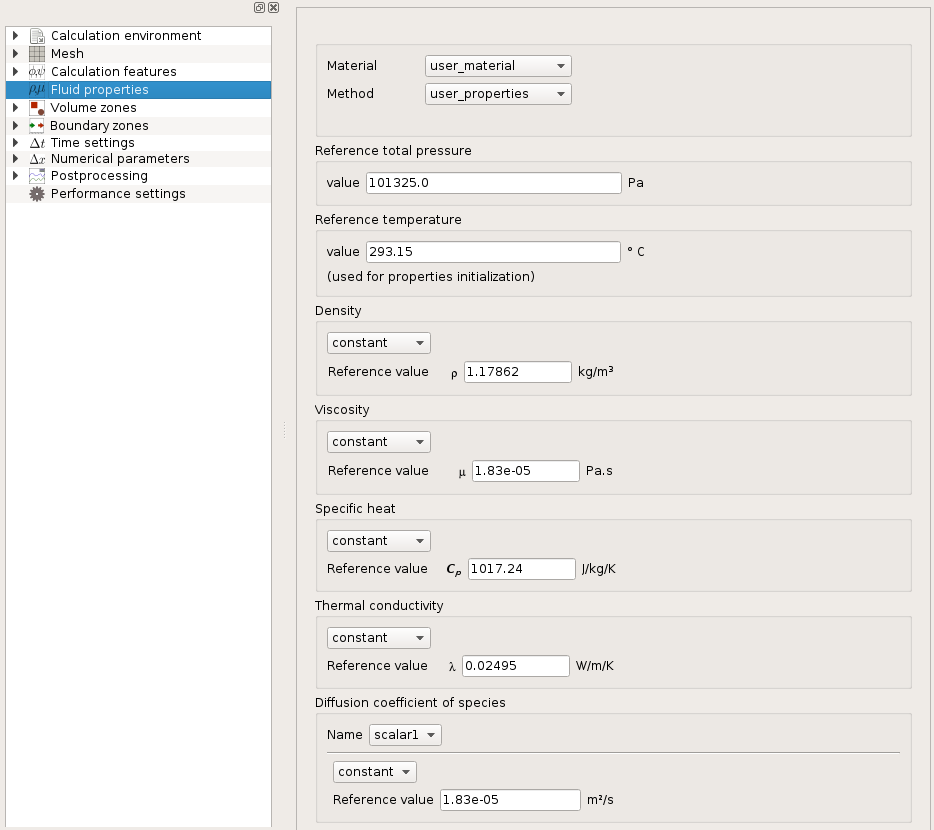
\includegraphics[width=0.9\textwidth]{gui_fluid_props}
\caption{Physical properties - Fluid properties}
\label{fig:gui_fluid_props2}
\end{center}
\end{figure}
%
\begin{figure}[!ht]
\begin{center}
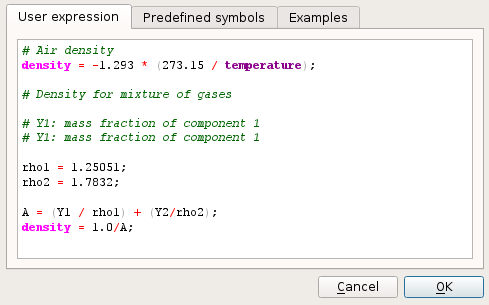
\includegraphics[width=10cm]{gui_density_law}
\caption{Definition of a user law for the density}
\label{fig:UL1_GUI}
\end{center}
\end{figure}

If necessary, all the variation laws related to the fluid physical properties are written in the subroutine \texttt{cs\_user\_physical\_properties}.

The validity of the variation laws must be checked, particularly when
non-linear laws are defined (for instance, a third-degree polynomial law
may produce negative density values).

{\bf \underline{WARNING}}\label{sec:prg_propvar}%
\begin{list}{$\bullet$}{}
\item If the user wishes to impose a variable density or variable viscosity in
      \texttt{usphyv}, it must be flagged either in the interface or in
      \texttt{cs\_user\_parameters.f90}(\texttt{irovar}=1, \texttt{ivivar}=1).
\item In order to impose a physical property ($\rho$, $\mu$,
      $\lambda$, $C_p$)\footnote{Except for some specific physics}, a reference
      value should be provided in the interface or in \texttt{cs\_user\_parameters.f90} (in
      particular for $\rho$, the pressure will be function of $\rho_0 gz$)
\item By default, the $C_p$ coefficient and the
      diffusivity for the scalars \texttt{iscal} ($\lambda_T$ for the
      temperature) are considered as constant in time and uniform in
      space, with the values \texttt{cp0} and \texttt{visls0(iscal)}
      specified in the interface or in \texttt{cs\_user\_parameters.f90}.\\
To assign a variable value to $C_p$, the user \textbf{must} specify it in the
      interface (with a user law) or assign the value 1 to \texttt{icp} in \texttt{cs\_user\_parameters.f90},
      and fill for each cell \texttt{iel} the array \texttt{cpro\_cp} which can be retrieved by calling
      \texttt{field\_get\_val\_s(icp, cpro\_cp)} in \texttt{cs\_user\_physical\_properties}.
      NB: completing the array \texttt{cpro\_cp} while \texttt{icp=0} induces array
      overwriting problems and produces wrong results.

\item In the same way, to have variable diffusivities for the scalars
      \texttt{iscal}, the user \textbf{must} specify it in the interface (with a user law) or calling \texttt{field\_set\_key\_int(ivarfl(isca(iscal)), kivisl, 0)}
      in \texttt{cs\_user\_parameters.f90} (in \texttt{usipsu}), and complete for each cell
      \texttt{iel} the values array of the field id \texttt{ifcvsl} returned by calling
      \texttt{field\_get\_key\_id(ivarfl(isca(iscal)), kivisl, ifcvsl)}
      in \texttt{cs\_user\_physical\_properties}.\\

{\em Note}: The scalar diffusivity id must not be defined for
      user scalars representing the average of the square of the
      fluctuations of another scalar, because the diffusivity of a user
      scalar \texttt{jj} representing the average of the square of the
      fluctuations of a user scalar \texttt{kk} comes directly from the
      diffusivity of this last scalar. In particular, the diffusivity
      of the scalar \texttt{jj} is variable if the diffusivity of \texttt{kk}
      is variable.
\end{list}


%==================================
\subsubsection{Modification of the turbulent viscosity}
%==================================

The subroutine \texttt{usvist} is used to modify the calculation of the turbulent
viscosity, {\em i.e.} $\mu_t$ in $kg.m^{-1}.s^{-1}$
(this piece of information, at the mesh cell centres, is conveyed by the
variable \texttt{cpro\_visct}  which can be retrieved by calling
\texttt{field\_get\_val\_s(ivisct, cpro\_cp)}). The
subroutine is called at the beginning of every time step, after the
calculation of the physical parameters of the flow and of the
``conventional'' value of $\mu_t$ corresponding to the chosen turbulence
model (indicator \texttt{iturb}).\\
{\em WARNING: The calculation of the turbulent viscosity being a
particularly sensible stage, a wrong use of {\em\texttt{usvist}} may
seriously distort the results.}

%==================================
\subsubsection{Modification of the variable $C$ of the dynamic LES model}
%==================================

\noindent
\textit{Subroutine called every time step in the case of LES with the
dynamic model.}

The subroutine \texttt{ussmag} is used to modify the calculation of the variable $C$ of
the LES sub-grid scale dynamic model.

It worth to recalling that the LES approach introduces the notion of
filtering between large eddies and small motions. The solved variables
are said to be filtered in an ``implicit'' way. Sub-grid scale models
(``dynamic'' models) introduce in addition an explicit filtering.

The notations used for the definition of the variable $C$ used in the
dynamic models of \CS are specified below. These notations are the ones
assumed in the document \cite{benhamadouche01}, to which the user may
refer to for more details.

The value of $a$ filtered by the explicit filter (of width
$\widetilde{\overline{\Delta}}$) is called $\widetilde{a}$ and the value
of $a$ filtered by the implicit filter (of width $\overline{\Delta}$) is
called $\overline{a}$.
We define:
\begin{equation}
\begin{array}{ll}
\overline{S}_{ij}=\frac{1}{2}(\frac{\partial \overline{u}_i}{\partial x_j}
                  +\frac{\partial \overline{u}_j}{\partial x_i})  &
||\overline{S}||=\sqrt{2 \overline{S}_{ij}\overline{S}_{ij}}\\
\alpha_{ij}=-2\widetilde{\overline{\Delta}}^2
             ||\widetilde{\overline{S}}||
             \widetilde{\overline{S}}_{ij}&
\beta_{ij}=-2\overline{\Delta}^2
             ||\overline{S}||
               \overline{S}_{ij}\\
L_{ij}=\widetilde{\overline{u}_i\overline{u}_j}-
 \widetilde{\overline{u}}_i\widetilde{\overline{u}}_j&
M_{ij}=\alpha_{ij}-\widetilde{\beta}_{ij}\\
\end{array}
\end{equation}


In the framework of LES, the total viscosity (molecular + sub-grid) in
$kg.m^{-1}.s^{-1}$ may be written in \CS:
\begin{equation}
\begin{array}{llll}
\mu_{\text{total}}&=&\mu+\mu_{\text{sub-grid}} &
    \text{\ \ if\ \ }\mu_{\text{sub-grid}}>0\\
                   &=&\mu                          &
    \text{\ \ otherwise }\\
\text{with\ }\mu_{\text{sub-grid}}&=&\rho C \overline{\Delta}^2 ||\overline{S}||
\end{array}
\end{equation}

$\overline{\Delta}$ is the width of the implicit filter, defined at the
cell $\Omega_i$ by \\
$\overline{\Delta}=XLESFL*(ALES*|\Omega_i|)^{BLES}$
\index{xlesfl}\index{ales}\index{bles}.

In the case of the Smagorinsky model (\texttt{iturb=40}), $C$ is a
constant which is worth $C_s^2$. $C_s^2$ is the so-called Smagorinsky
constant and is stored in the variable \texttt{$csmago$\index{csmago}}.

In the case of the dynamic model (\texttt{iturb=41}), $C$ is variable in
time and in space. It is determined by
$\displaystyle C=\frac{M_{ij}L{ij}}{M_{kl}M_{kl}}$.

In practice, in order to increase the stability, the code does not use the
value of $C$ obtained in each cell, but an average with the values
obtained in the neighbouring cells (this average uses the extended
neighbourhood and corresponds to the explicit filter). By default, the
value calculated by the code is
\begin{displaymath}
C=\frac{\widetilde{M_{ij}L{ij}}}{\widetilde{M_{kl}M_{kl}}}
\end{displaymath}

The subroutine \texttt{ussmag} allows to modify this value. It is for
example possible to calculate the local average after having calculated the
ratio
\begin{displaymath}
C=\widetilde{\left[\frac{M_{ij}L{ij}}{M_{kl}M_{kl}}\right]}
\end{displaymath}

{\em WARNING: The subroutine {\em\texttt{ussmag}} can be activated only when
the dynamic model is used.}

%==================================
\subsection{User source terms}
%==================================
\label{sec:prg_usersourceterms}

Assume, for example, that the user source terms modify the equation of a
variable $\varphi$ in the following way:
\begin{displaymath}
\rho\frac{\partial \varphi}{\partial t}+\ldots = \ldots + S_{impl}\times\varphi+S_{expl}
\end{displaymath}
The example is valid for a velocity component, for a turbulent variable ($k$, $\varepsilon$, $R_{ij}$, $\omega$,
$\varphi$ or $\overline{f}$) and for a scalar (or for the average of the
square of the fluctuations of a scalar), because the syntax of all the
subroutines \texttt{ustsnv}, \texttt{cs\_user\_turbulence\_source\_terms}
 and \texttt{ustssc} in the \texttt{cs\_user\_source\_terms} file is similar.

In the finite volume formulation, the solved system is then modified as
follows:
\begin{displaymath}
\left(\frac{\rho_i\Omega_i}{\Delta t_i}-\Omega_iS_{impl,i}\right)
\left(\varphi_i^{(n+1)}-\varphi_i^{(n)}\right)
+\ldots = \ldots + \Omega_iS_{impl,i}\varphi_i^{(n)} + \Omega_iS_{expl,i}
\end{displaymath}
The user needs therefore to provide the following values:\\
$\text{\texttt{crvimp}}_i=\Omega_iS_{impl,i}$\\
$\text{\texttt{crvexp}}_i=\Omega_iS_{expl,i}$

In practice, it is essential for the term
$\displaystyle \left(\frac{\rho_i\Omega_i}{\Delta
t_i}-\Omega_iS_{impl,i}\right)$ to be positive. To ensure this property,
the equation really taken into account by the code is the following:
\begin{displaymath}
\left(\frac{\rho_i\Omega_i}{\Delta t_i}-
\text{Min}(\Omega_iS_{impl,i};0)\right)
\left(\varphi_i^{(n+1)}-\varphi_i^{(n)}\right)
+\ldots = \ldots + \Omega_iS_{impl,i}\varphi_i^{(n)} + \Omega_iS_{expl,i}
\end{displaymath}
To make the ``implicitation'' effective, the source term decomposition
between the implicit and explicit parts will be done by the user who must
ensure that $\text{\texttt{crvimp}}_i=\Omega_iS_{impl,i}$ is always negative
(otherwise the solved equation remains right, but there will not be
``implicitation'').

{\em WARNING: When the second-order in time is used along with the extrapolation of the
source terms\footnote{indicator \texttt{isno2t} for the velocity,
\texttt{isto2t} for the turbulence and \texttt{isso2t} for the scalars}, it is no longer possible to test the sign of $S_{impl,i}$,
because of coherence reasons (for more details, the user may refer to
the theoretical and computer documentation \cite{theory} of the
subroutine \texttt{preduv}). The user must therefore make sure it is
always positive (or take the risk to affect the calculation stability).}

\minititre{Particular case of a linearised source term}

In some cases, the added source term is not linear, but the user may
want to linearise it using a first-order Taylor development, in order to
make it partially implicit.\\
Consider an equation of the type:
\begin{displaymath}
\rho\frac{\partial\varphi}{\partial t}=F(\varphi)
\end{displaymath}
To make it implicit using the following method:
\begin{eqnarray*}
\frac{\rho_i\Omega_i}{\Delta t}\left(\varphi_i^{(n+1)}-\varphi_i^{(n)}\right) & = &
\Omega_i\left[F(\varphi_i^{(n)})+\left(\varphi_i^{(n+1)}-\varphi_i^{(n)}\right)
\frac{dF}{d\varphi}(\varphi_i^{(n)})\right]\\
& = & \Omega_i\frac{dF}{d\varphi}(\varphi_i^{(n)})\times\varphi_i^{(n+1)}
+\Omega_i\left[F(\varphi_i^{(n)})-\frac{dF}{d\varphi}(\varphi_i^{(n)})
\times\varphi_i^{(n)}\right]
\end{eqnarray*}

The user must therefore specify:\\
$\displaystyle\text{\texttt{crvimp}}_i=\Omega_i\frac{dF}{d\varphi}(\varphi_i^{(n)})$\\
$\displaystyle\text{\texttt{crvexp}}_i=
\Omega_i\left[F(\varphi_i^{(n)})-\frac{dF}{d\varphi}(\varphi_i^{(n)})\times\varphi_i^{(n)}\right]$

\underline{\em Example}:\\
If the equation is
$\displaystyle \rho\frac{\partial\varphi}{\partial t}=-K\varphi^2$,
the user must set:\\
$\text{\texttt{crvimp}}_i=-2K\Omega_i\varphi_i^{(n)}$\\
$\text{\texttt{crvexp}}_i=K\Omega_i[\varphi_i^{(n)}]^2$

%==================================
\subsubsection{In Navier-Stokes}
%==================================

The source term in Navier-Stokes can be filled in thanks to the GUI or the
\texttt{cs\_user\_source\_terms} user file.
Without the GUI, the subroutine \texttt{ustsnv} is used to
add user source terms to the Navier-Stokes equations (at each time step).

\texttt{ustsnv} is called only once per time step; for each cell \texttt{iel},
the vector \texttt{crvexp(.,iel)} (explicit part) and the matrix \texttt{crvimp(.,.,iel)}
(implicit part) must be filled in for the whole velocity vector.


%==================================
\subsubsection{For $k$ and $\varepsilon$}
%==================================

\noindent
\textit{Subroutine called every time step, for the $k-\varepsilon$ and
the v2f models.}

The subroutine \texttt{cs\_user\_turbulence\_source\_terms} is used to add source terms to the transport equations
related to the turbulent kinetics energy $k$ and to the turbulent
dissipation $\varepsilon$.
This subroutine is called every time step (the
treatment of the two variables $k$ and $\varepsilon$ is made
simultaneously). The user is expected to provide the arrays \texttt{crkimp} and
\texttt{crkexp} for $k$, and \texttt{creimp} and \texttt{creexp} for
$\varepsilon$. These arrays are similar to the arrays \texttt{crvimp} and
\texttt{crvexp} given for the velocity in the user subroutine \texttt{ustsnv}.
The way of making implicit the resulting source terms is the same as the one
presented in \texttt{ustsnv}. For $\varphi$ and $\bar{f}$
in the v2f model, see \texttt{cs\_user\_turbulence\_source\_terms}, \S\ref{sec:prg_ustsv2}.

%==================================
\subsubsection{For $R_{ij}$ and $\varepsilon$}
%==================================

\noindent
\textit{Subroutine called every time step, for the $R_{ij}-\varepsilon$ models.}

The subroutine \texttt{cs\_user\_turbulence\_source\_terms} is used to add source terms to the transport equations
related to the Reynolds stress variables $R_{ij}$ and to the turbulent
dissipation $\varepsilon$.
This subroutine is called 7 times every time step
(once for each Reynolds stress component and once for the
dissipation). The user must provide the arrays \texttt{crvimp} and
\texttt{crvexp} for the field variable of index \texttt{f\_id} (referring successively to
\texttt{ir11}, \texttt{ir22}, \texttt{ir33},
\texttt{ir12}, \texttt{ir13}, \texttt{ir23} and
\texttt{iep}). These arrays are similar to the arrays \texttt{crvimp}
and \texttt{crvexp} given for the velocity in the user subroutine
\texttt{ustsnv}. The method for impliciting the resulting source terms is the
same as that presented in \texttt{ustsnv}.

%==================================
\subsubsection{For $\varphi$ and $\overline{f}$}
%==================================
\label{sec:prg_ustsv2}

\noindent
\textit{Subroutine called every time step, for the v2f models.}

The subroutine \texttt{cs\_user\_turbulence\_source\_terms} is used to add source terms to the transport equations
related to the variables $\varphi$ and $\overline{f}$ of the v2f
$\varphi$-model. This subroutine is called twice
every time step (once for $\varphi$ and once for $\overline{f}$).
The user is expected to provide the arrays \texttt{crvimp} and
\texttt{crvexp} for \texttt{ivar} referring successively to \texttt{iphi}
and \texttt{ifb}. Concerning $\varphi$, these arrays are similar to the arrays
\texttt{crvimp} and \texttt{crvexp} given for the velocity in the user subroutine
\texttt{ustsnv}. Concerning $\overline{f}$, the equation is slightly
different:
\begin{displaymath}
L^2 div(\grad(\overline{f})) = \overline{f} + \ldots + S_{impl}\times\overline{f}+S_{expl}
\end{displaymath}
In the finite volume formulation, the solved system is written as:
\begin{displaymath}
\int_{\partial\Omega_i}\grad(\overline{f})^{(n+1)}dS=\frac{1}{L_i^2}\left(
\Omega_i\overline{f}^{(n+1)}_i + \ldots +  \Omega_iS_{impl,i}\overline{f}_i^{(n+1)} +
\Omega_iS_{expl,i} \right)
\end{displaymath}
The user must then specify:\\
$\text{\texttt{crvimp}}_i=\Omega_iS_{impl,i}$\\
$\text{\texttt{crvexp}}_i=\Omega_iS_{expl,i}$

The way of making implicit the resulting source terms is the same as the
one presented in \texttt{ustsnv}.

%==================================
\subsubsection{For $k$ and $\omega$}
%==================================

\noindent
\textit{Subroutine called every time step, for the $k-\omega$ SST model.}

The subroutine \texttt{cs\_user\_turbulence\_source\_terms} is used to add source terms to the transport equations
related to the turbulent kinetics energy $k$ and to the specific
dissipation rate $\omega$. This subroutine is
called every time step (the treatment of the two
variables $k$ and $\omega$ is made simultaneously). The user is expected
to provide the arrays \texttt{crkimp} and \texttt{crkexp} for the variable
$k$, and the arrays \texttt{crwimp} and \texttt{crwexp} for the variable $\omega$.
These arrays are similar to the arrays \texttt{crvimp} and \texttt{crvexp}
given for the velocity in the user subroutine \texttt{ustsnv}. The way of
making implicit the resulting source terms is the same as the one presented in
\texttt{ustsnv}.

%==================================
\subsubsection{For $\tilde{\nu}_t$}
%==================================

\noindent
\textit{Subroutine called every time step, or the Spalart-Allmaras model.}

The subroutine \texttt{cs\_user\_turbulence\_source\_terms} is used to add source terms to the transport equations
related to the turbulent viscosity $\nu_t$ for the Spalart-Allmaras model.
This subroutine is called every time step. The user is expected
to provide the arrays \texttt{crkimp} and \texttt{crkexp} for the variable
$\tilde{\nu}_t$. These arrays are similar to the arrays \texttt{crvimp} and \texttt{crvexp}
given for the velocity in the user subroutine \texttt{ustsnv}. The way of
making implicit the resulting source terms is the same as the one presented in
\texttt{ustsnv}.

%==================================
\subsubsection{For user scalars}
%==================================

\noindent
\textit{Subroutine called every time step.}

The source terms in the transport equations related to the user scalars
(passive or not, average of the square of the fluctuations of a scalar, ...)
can be filled in thanks to the GUI or the \texttt{cs\_user\_source\_terms} user file.
Without the GUI, the subroutine \texttt{ustssc} is used to add source terms to the
transport equations related to the user scalars. In the same way as
\texttt{ustsnv}, this subroutine is called every time step, once for
each user scalar. The user must provide the arrays \texttt{crvimp}
and \texttt{crvexp} related to each scalar. \texttt{cvimp} and \texttt{crvexp}
must be set to 0 for the scalars on which it is not wished for the user source
term to be applied (the arrays are initially set to 0 at each inlet in the subroutine).

%==================================
\subsection{Pressure drops (head losses) and porosity}
%==================================
\label{sec:prg_headlosses}

%==================================
\subsubsection{Head losses}
%==================================

Pressure drops can be defined in the Graphical User Interface (GUI) or in the user sources. In the GUI, the page ``Volume zones'' allows to define areas where pressure drops are applied, see an example in fig \ref{fig:hl1}. The item ``Head losses'' allows to specify the head loss coefficients, see \figurename~\ref{fig:hl2}. The tensor representing the pressure drops is supposed to be symmetric
and positive.

\begin{figure}[!ht]
\begin{center}
%\begin{tabular}{c}
%\includegraphics[width=14cm]{gui_volume_regions} \\
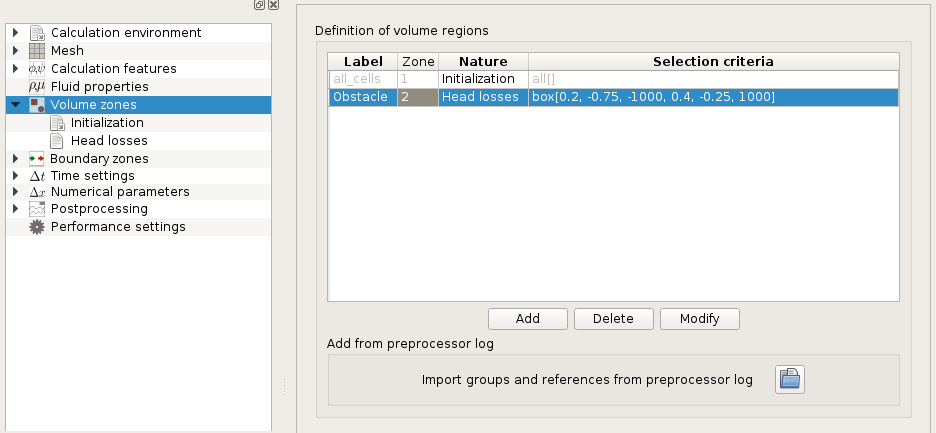
\includegraphics[width=0.9\textwidth]{gui_head_loss_regions}
%\end{tabular}
\caption{Creation of head losses region}
\label{fig:hl1}
\end{center}
\end{figure}
%
\begin{figure}[!ht]
\begin{center}
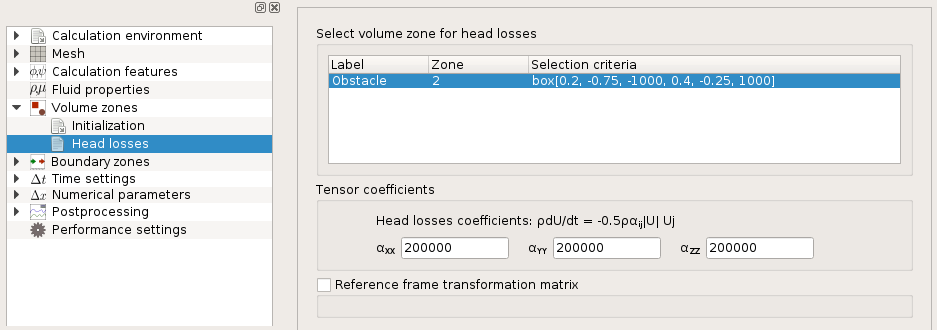
\includegraphics[width=0.9\textwidth]{gui_head_loss_coeffs}
\caption{Head losses coefficients}
\label{fig:hl2}
\end{center}
\end{figure}

In the user sources, two files can be of use: \texttt{cs\_user\_zones.c} (called at the computation start) to define a volume zone and \texttt{cs\_user\_head\_losses.c} (called at each iteration) to specify the values of the head losses coefficients. Note that volume zones defined with the GUI are available in \texttt{cs\_user\_head\_losses.c}.

See the associated \doxygenfile{cs_head_losses.html}{\texttt{doxygen}} documentation for examples.

%==================================
\subsubsection{Porosity}
%==================================

Porous zones can be set through the GUI in the ``Volume zones'' page. Alternatively, porous zones can be defined in the user source
\texttt{cs\_user\_porosity.c} and the porous model shall be chosen by setting the keyword \texttt{iporos} in
\texttt{cs\_user\_parameters} file. See the associated \doxygenfile{cs_porosity.html}{\texttt{doxygen}} documentation for examples.
Porous zones are defined at the beginning of the computation once and for all.\\

%==================================
\subsection{Management of the mass sources}
%==================================

The subroutine \texttt{cs\_user\_mass\_source\_terms} is used to add a density source term in some cells of
the domain (called at each time step). The mass conservation equation is then modified as follows:
\begin{displaymath}
\frac{\partial \rho}{\partial t} + div(\rho\vect{u})=\Gamma
\end{displaymath}

$\Gamma$ is the mass source term expressed in $kg.m^{-3}.s^{-1}$.

The presence of a mass source term modifies the evolution equation of
the other variables, too. Let $\varphi$ be any solved variable apart
from the pressure (velocity component, turbulent energy, dissipation,
scalar, ...). Its evolution equation becomes:
\begin{displaymath}
\rho\frac{\partial \varphi}{\partial t} + \ldots = \ldots + \Gamma(\varphi_i-\varphi)
\end{displaymath}

$\varphi_i$ is the value of $\varphi$ associated with the mass entering
or leaving the domain. After discretisation, the equation may be written:
\begin{displaymath}
\rho\frac{\varphi^{(n+1)}-\varphi^{(n)}}{\Delta t} + \ldots
= \ldots + \Gamma(\varphi_i-\varphi^{(n+1)})
\end{displaymath}

For each variable $\varphi$, there are two possibilities:
\begin{list}{$\bullet$}{}
\item We can consider that the mass is added (or removed) with the
      ambient value of $\varphi$. In this case
      $\varphi_i=\varphi^{(n+1)}$ and the equation of $\varphi$ is not
      modified.
\item Or we can consider that the mass is added with an
      imposed value $\varphi_i$ (this solution is physically correct
      only when the mass is effectively added, $\Gamma>0$).
\end{list}

\bigskip

This subroutine is called three times every time step.

\begin{list}{$\bullet$}{}
\item During the first call, all the cells are checked to know the
      number of cells containing a mass source term.
      This number is called \texttt{ncesmp\index{ncesmp}} in
      \texttt{cs\_user\_mass\_source\_terms} (and corresponds to
      \texttt{ncetsm\index{ncetsm}}). It is used to lay out the arrays
      related to the mass sources. If there is no mass source,
      \texttt{ncesmp} must be equal to zero (it is the default value, and the
      rest of the subroutine is then useless).

\item During the second call, all the cells are checked again to
      complete the array \texttt{icetsm\index{icetsm}} whose dimension is
      \texttt{ncesmp}. \mbox{\texttt{icetsm(ieltsm)}} is the number of the
      \texttt{ieltsm}\raisebox{1ex}{\small th} cell containing a mass source.

\item During the third call, all the cells containing mass sources are
      checked in order to complete the arrays
      \mbox{\texttt{itypsm(ncesmp,nvar)}\index{itypsm}} and
      \mbox{\texttt{smacel(ncesmp,nvar)}\index{smacel}}:\\
- \texttt{itypsm(ieltsm,ivar)} is the flow type associated with the variable
      \texttt{ivar} in the \texttt{ielstm}\raisebox{1ex}{\small th} cell
      containing a mass source.\\
\hspace*{1cm}\texttt{itypsm}=0: $\varphi_i=\varphi^{(n+1)}$ condition\\
\hspace*{1cm}\texttt{itypsm}=1: imposed $\varphi_i$ condition\\
\hspace*{1cm}\texttt{itypsm} is not used for \texttt{ivar=ipr}\\
- \texttt{smacel(ieltsm,ipr)} is the value of the mass source term $\Gamma$, in
$kg.m^{-3}.s^{-1}$.\\
- \texttt{smacel(ieltsm,ivar)}, for \texttt{ivar} different from
\texttt{ipr}, is the value
of $\varphi_i$ for the variable \texttt{ivar} in the
\texttt{ielstm}\raisebox{1ex}{\small th} cell containing a mass source.\\

\minititre{Notes}
$\bullet$ If \texttt{itypsm(ieltsm,ivar)=0}, \texttt{smacel(ieltsm,ivar)}
      is not used.\\
$\bullet$ If $\Gamma$=\texttt{smacel(ieltsm,ipr)}$<$0, mass is removed from
      the system, and \CS considers automatically a
      $\varphi_i=\varphi^{(n+1)}$ condition, whatever the values given
      to \texttt{itypsm(ieltsm,ivar)} and \texttt{smacel(ieltsm,ivar)}
      (the extraction of a variable is done at ambient value).
\end{list}

The three calls are made every time step, so that variable mass source
zones or values may be treated.\\

For the variance, do not take into account the scalar $\varphi_i$ in the environment
where $\varphi\ne\varphi_i$ generates a variance source.

%==================================
\subsection{User law editor of the GUI}
%==================================

A formula interpreter is embedded in \CS, which can be used through the GUI.
In order to call the formula editor of the GUI, click on the button:

\begin{figure}[!ht]
\begin{center}
\includegraphics[width=1cm]{gui_formula_button}
\label{fig:mei_button}
\end{center}
\end{figure}

The formula editor is a window with three tabs:
\begin{list}{$\bullet$}{}
\item User expression

This tab is the formula editor. At the opening of the
window only the required symbols are displayed.
The syntax colorization shows to the user symbols which are
required symbols, functions, or user variables.
Each expression must be closed by a semicolon (``;''). The
required symbols must be present in the final user law. A
syntax checker is used when the user clicks on the OK button.

\begin{figure}[!ht]
\begin{center}
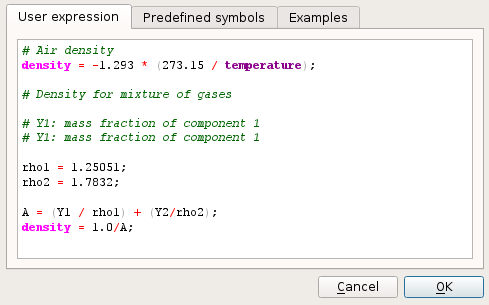
\includegraphics[width=10cm]{gui_density_law}
\caption{Example of the user law editor}
\label{fig:mei_editor}
\end{center}
\end{figure}

\item Predefined symbols

There are three types of symbols \\

\underline{Useful functions:}

\texttt{cos}: cosine

\texttt{sin}: sine

\texttt{tan}: tangent

\texttt{exp}: exponential

\texttt{sqrt}: square root

\texttt{log}: Napierian logarithm

\texttt{acos}: arc cosine

\texttt{asin}: arc sine

\texttt{atan(x)}: arc tangent (arc tangent of x in radians; the return value is in the range [-pi/2, pi/2])

\texttt{atan2(y,x)}: arc tangent (arc tangent of y/x in radians; the return value is in the range [-pi, pi])

\texttt{cosh}: hyperbolic cosine

\texttt{sinh}: hyperbolic sine

\texttt{tanh}: hyperbolic tangent

\texttt{abs}: absolute value

\texttt{mod}: modulo

\texttt{int}: floor

\texttt{min}: minimum

\texttt{max}: maximum

\underline{Useful constants:}

pi = 3.14159265358979323846

e = 2.718281828459045235\\


\underline{Operators and statements:}

$+$ \qquad$-$\qquad $*$\qquad $/$ \qquad$\wedge$

! \qquad $<$ \qquad $>$ \qquad $<=$ \qquad $>=$ \qquad $==$ \qquad $!=$ \qquad $\&\&$ \qquad $\mid\mid$

\texttt{while} \texttt{if} \texttt{else} \texttt{print}


\item Examples

This tab displays examples of formula, which could be copy and paste.

\end{list}
%==================================
\subsection{Modification of the variables at the end of a time step}
%==================================

The subroutine \texttt{cs\_user\_extra\_operations} is called at the end
of every time step. It is used to print of modify any variable at the end
of every time step.

Several examples are given in the directory \texttt{EXAMPLES}:
\begin{list}{-}{}
\item Calculation of a thermal balance at  the boundaries and in the
      domain (including the mass source terms)

\item Modification of the temperature in a given area starting from a
      given time

\item Extraction of a 1D profile (which is also possible with the GUI,
see \figurename~\ref{fig:gui_output_profiles})

\item Printing of a moment

\item Usage of utility
      subroutines in the case of a parallel calculation
      (calculation of a sum on the processors, of a maximum, ...)
\end{list}

{\em WARNING: As all the variables (solved variables, physical
properties, geometric parameters) can be modified in this subroutine, a
wrong use may distort totally the calculation.}

The thermal balance example is particularly interesting.
\begin{list}{-}{}
\item It can be easily adapted to another scalar (only three simple
      modifications to do, as indicated in the subroutine).
\item It shows how to make a sum on all the sub-domains in the framework
      of a parallel calculation (see the calls to the subroutines
      \texttt{par*}).
\item It shows the precautions to take before doing some operations in
      the framework of periodic or parallel calculations (in particular
      when we want to calculate the gradient of a variable or to have
      access to values at the neighbouring cells of a face).
\item Finally it must not be forgotten that the resolution with
      temperature (and not enthalpy) as a solved variable is questionable when the specific
      heat is not constant.
\end{list}

%==================================
\section{Advanced modelling setup}
%==================================

%==================================
\subsection{Use of a specific physics}
%==================================
\label{sec:prg_usppmo}%
Specific physics such as dispersed phase, atmospheric flows, gas combustion,
pulverised fuel combustion, electrical model and compressible model can be
added by the user from the interface, or by using the subroutine \texttt{usppmo} of
the \texttt{cs\_user\_parameters} file (called only during the calculation initialisation).
With the interface, when a specific physics is activated in \figurename~\ref{fig:5_GUI},
additional items or headings may appear (see for instance Sections \ref{sec:Ini-lag}
and \ref{sec:Ini-coal}).

\begin{figure}[!ht]
\begin{center}
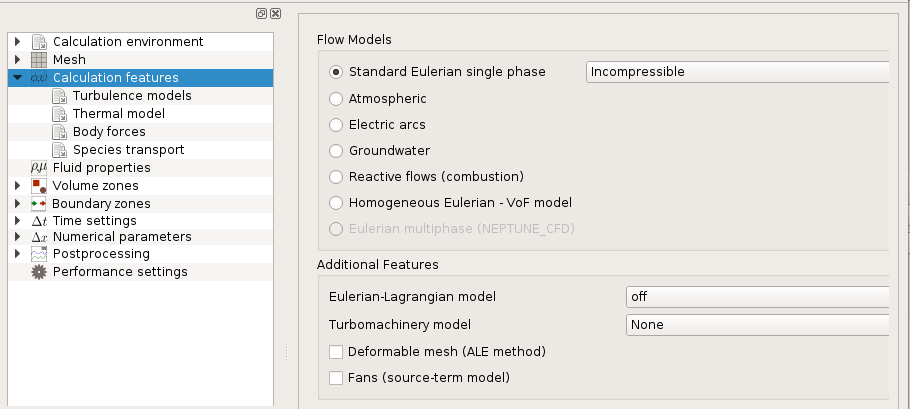
\includegraphics[width=0.9\textwidth]{gui_calculation_features}
\caption{Specific physics models selection}
\label{fig:5_GUI}
\end{center}
\end{figure}

When the interface is not used, \texttt{usppmo} is one of the three subroutines
which must be obligatory completed by the user in order to use a specific physics module
(only heavy fuel combustion is not available with the GUI).
At the moment, \CS allows to use two ``pulverised coal'' modules
(with Lagrangian coupling or not) and one ``pulverised heavy fuel'' module,
two ``gas combustion'' modules, two ``electrical'' modules,
a ``compressible'' module and an ``atmospheric'' module. To activate one of
these modules, the user must complete one (and only one) of the
indicators \texttt{ippmod(i.....)\index{ippmod}} in the subroutine
\texttt{usppmo}. By default, all the indicators \texttt{ippmod(i.....)} are
initialised at -1, which means that no specific physics is activated.

\begin{list}{$\bullet$}{}
       \item Diffusion flame in the framework of ``3 points'' rapid complete
             chemistry: indicator {\bf \tt ippmod(icod3p\index{icod3p})}
        \begin{list}{$\rightarrow$}{}
               \item \texttt{ippmod(icod3p)} = 0 adiabatic conditions
               \item \texttt{ippmod(icod3p)} = 1 permeatic conditions (enthalpy
                     transport)
               \item \texttt{ippmod(icod3p)} =-1 module not activated
         \end{list}
        \item Eddy Break Up pre-mixed flame: indicator {\bf \tt
             ippmod(icoebu\index{icoebu})}
         \begin{list}{$\rightarrow$}{}
                \item \texttt{ippmod(icoebu\index{icoebu})} = 0 adiabatic
                      conditions at constant richness
                \item \texttt{ippmod(icoebu)} = 1 permeatic conditions at
                      constant richness
                \item \texttt{ippmod(icoebu)} = 2 adiabatic conditions at
                      variable richness
                \item \texttt{ippmod(icoebu)} = 3 permeatic conditions at
                      variable richness
                \item \texttt{ippmod(icoebu)} =-1 module not activated
         \end{list}
        \item Libby-Williams pre-mixed flame: indicator {\bf \tt ippmod(icolwc\index{icolwc})}
         \begin{list}{$\rightarrow$}{}
               \item \texttt{ippmod(icolwc)}=0 two peak model with adiabiatic conditions.
               \item \texttt{ippmod(icolwc)}=1 two peak model with permeatic conditions.
               \item \texttt{ippmod(icolwc)}=2 three peak model with adiabiatic conditions.
               \item \texttt{ippmod(icolwc)}=3 three peak model with permeatic conditions.
               \item \texttt{ippmod(icolwc)}=4 four peak model with adiabiatic conditions.
               \item \texttt{ippmod(icolwc)}=5 four peak model with permeatic conditions.
               \item \texttt{ippmod(icolwc)}=-1 module not activated.
          \end{list}
        \item Multi-coals and multi-classes pulverised coal combustion:
              indicator {\bf \tt ippmod(iccoal\index{iccoal})}
              The number of different coals must be less than or equal to
              \texttt{ncharm\index{ncharm}} = 3. The number of particle size
             classes \texttt{nclpch\index{nclpch}(icha)} for the coal
             \texttt{icha}, must
             be less than or equal to \texttt{ncpcmx\index{ncpcmx}} = 10.
         \begin{list}{$\rightarrow$}{}
                \item \texttt{ippmod(iccoal)} = 0 imbalance between the
                      temperature of the continuous and the solid phases
                \item \texttt{ippmod(iccoal)} = 1 otherwise
                \item \texttt{ippmod(iccoal)} =-1 module not activated
         \end{list}

        \item Multi-classes pulverised heavy fuel combustion:
              indicator {\bf \tt ippmod(icfuel\index{icfuel})}
         \begin{list}{$\rightarrow$}{}
                \item \texttt{ippmod(icfuel)} = 0 module activated
                \item \texttt{ippmod(icfuel)} =-1 module not activated
         \end{list}

        \item Lagrangian modelling of multi-coals and
             multi-classes pulverised coal combustion:
                 indicator {\bf \tt ippmod(icpl3c\index{icpl3c})}
              The number of different coals must be less than or equal to
              \texttt{ncharm\index{ncharm}} = 3. The number of particle size
             classes \texttt{nclpch\index{nclpch}(icha)} for the coal
             \texttt{icha}, must be less than or equal to
             \texttt{ncpcmx\index{ncpcmx}} = 10.
         \begin{list}{$\rightarrow$}{}
                \item \texttt{ippmod(icpl3c)} = 1 coupling with the Lagrangian
                      module, with transport of $H_2$
                \item \texttt{ippmod(icpl3c)} =-1 module not activated
         \end{list}
       \item Electric arcs module (Joule effect and Laplace forces):
             indicator {\bf \tt ippmod(ielarc\index{ielarc})}
        \begin{list}{$\rightarrow$}{}
               \item \texttt{ippmod(ielarc)} = 1 determination of the magnetic field by
                     means of the Ampere's theorem (not available)
               \item \texttt{ippmod(ielarc)} = 2 determination of the magnetic
                     field by means of the vector potential
               \item \texttt{ippmod(ielarc)} =-1 module not activated
         \end{list}
       \item Joule effect module (Laplace forces not taken into account):
             indicator {\bf \tt ippmod(ieljou\index{ieljou})}
        \begin{list}{$\rightarrow$}{}
               \item \texttt{ippmod(ieljou)} = 1 use of a real potential
               \item \texttt{ippmod(ieljou)} = 2 use of a complex potential
               \item \texttt{ippmod(ieljou)} = 3 use of real potential and specific boundary conditions for transformers.
               \item \texttt{ippmod(ieljou)} = 4 use of complex potential and specific boundary conditions for transformers.
               \item \texttt{ippmod(ieljou)} =-1 module not activated
         \end{list}
       \item Compressible module: indicator {\bf \tt
             ippmod(icompf\index{icompf})}
        \begin{list}{$\rightarrow$}{}
               \item \texttt{ippmod(icompf)} = 0 module activated
               \item \texttt{ippmod(icompf)} =-1 module not activated
         \end{list}
       \item Atmospheric flow module: indicator {\bf \tt
             ippmod(iatmos\index{icompf})}
        \begin{list}{$\rightarrow$}{}
               \item \texttt{ippmod(iatmos)} =-1 module not activated
               \item \texttt{ippmod(iatmos)} = 0 standard modelling
               \item \texttt{ippmod(iatmos)} = 1 dry atmosphere
               \item \texttt{ippmod(iatmos)} = 2 humid atmosphere
         \end{list}
%       \item cooling towers module: indicator {\bf \tt
%             ippmod(iaeros\index{icompf})}
%        \begin{list}{$\rightarrow$}{}
%               \item \texttt{ippmod(iaeros\index)} =-1 module not activated
%               \item \texttt{ippmod(iaeros\index)} = 0 no model (NOT functional)
%               \item \texttt{ippmod(iaeros\index)} = 1 Poppe's model
%               \item \texttt{ippmod(iaeros\index)} = 2 Merkel's model
%         \end{list}
\end{list}

{\em WARNING: Only one specific physics module can be activated at the
same time.}

In the framework of the gas combustion modelling, the user may impose
his own enthalpy-temperature tabulation (conversion law). He needs then
to give the
value zero to the indicator \texttt{indjon\index{indjon}} (the default value
being 1). For more details, the user may refer to the following note
(thermochemical files).

\minititre{Note: the thermo-chemical files}
The user must not forget to place in the directory DATA the
thermochemical file \texttt{dp\_C3P}, \texttt{dp\_C3PSJ} or
\texttt{dp\_ELE} (depending on the specific physics module he activated)
Some example files are placed in the directory \texttt{DATA/REFERENCE} at the creation of the
study case. Their content is described below.

\begin{list}{$\bullet$}{}
       \item Example of file for the gas combustion:
        \begin{list}{$\rightarrow$}{}
               \item if the enthalpy-temperature conversion data base
                     JANAF is used: \texttt{dp\_C3P} (see
                     array \ref{tab:dpC3P}).

\begin{table}[htbp]
\begin{center}
\small{
\begin{tabular}{|c|c|c|c|} \hline
 Lines  &Examples of values &        Variables             & Observations                                     \\ \hline
  1     &         5         &  \texttt{ngaze\index{ngaze}} & Number of current species                        \\ \hline
  2     &        10         &   \texttt{npo\index{npo}}    & Number of points for the                         \\
        &                   &                              & enthalpy-temperature table                       \\ \hline
  3     &       300.        &  \texttt{tmin\index{tmin}}   & Lower temperature limit                          \\
        &                   &                              & for the table                                    \\ \hline
  4     &      3000.        &  \texttt{tmax\index{tmax}}   & Upper temperature limi   t                       \\
        &                   &                              & for the tabulation                               \\ \hline
  5     &                   &                              & Empty line                                       \\ \hline
  6     & CH4 O2 CO2 H2O N2 &  \texttt{nomcoe\index{nomcoe}}(\texttt{ngaze}) & List of the current species                      \\ \hline
  7     &.35 .35 .35 .35 .35&  \texttt{kabse\index{kabse}}(\texttt{ngaze})   & Absorption coefficient                           \\
        &                   &                              & of  the current species                          \\ \hline
  8     &         4         &  \texttt{nato\index{nato}}   & Number of elemental species                      \\ \hline
  9     &.012  1  0  1  0  0& \texttt{wmolat\index{wmolat}}(\texttt{nato}),  & Molar mass of the elemental                      \\
 10     &.001  4  0  0  2  0&                              & species (first column)                           \\
 11     &.016  0  2  2  1  0&\texttt{atgaze\index{atgaze}}(\texttt{ngaze},\texttt{nato})& Composition of the current species             \\
 12     &.014  0  0  0  0  2&                              & as a function of the elemental species           \\
        &                   &                              & (\texttt{ngaze} following columns)                        \\ \hline
 13     &         3         &  \texttt{ngazg\index{ngazg}} & Number of global species                         \\
        &                   &                              & Here, \texttt{ngazg} = 3 (Fuel, Oxidiser and Products)    \\ \hline
 14     &  1. 0. 0. 0. 0.   &                              & Composition of the global species as a           \\
 15     &  0. 1. 0. 0. 3.76 &\texttt{compog\index{compog}}(\texttt{ngaze},\texttt{ngazg})& function of the current species of line 6 \\
 16     &  0. 0. 1. 2. 7.52 &                              & In the order: Fuel (line 15),                    \\
        &                   &                              & Oxidiser (line 16) and Product (line 17)         \\ \hline
 17     &         1         &  \texttt{nrgaz\index{nrgaz}} & Number of global reactions                       \\
        &                   &                              & Here \texttt{nrgaz} = 1 (always equal to 1                \\
        &                   &                              & in this version)                                 \\ \hline
 18     &                   & \texttt{igfuel\index{igfuel}}(\texttt{nrgaz}), & Numbers of the global species concerned by       \\
        & 1 2 -1 -9.52 10.52&  \texttt{igoxy\index{igoxy}}(\texttt{nrgaz}),  & the stoichiometric ratio                         \\
        &                   &                              & (first 2 integers)                               \\
        &                   &\texttt{stoeg\index{stoeg}}(\texttt{ngazg},\texttt{nrgaz})& Stoichiometry in global species reaction.       \\
        &                   &                               & Negative for the reactants (here                \\
        &                   &                               & ``Fuel'' and ``Oxidiser'') and positive for      \\
        &                   &                               & the products (here ``Products'')                \\ \hline
\end{tabular}
}
\caption{Example of file for the gas combustion when JANAF is used: \texttt{dp\_C3P}}\label{tab:dpC3P}
\end{center}
\end{table}

               \item if the user provides his own enthalpy-temperature tabulation
                     (there must be three chemical species and only
                     one reaction): \texttt{dp\_C3PSJ} (see
                     array \ref{tab:dpC3PSJ}). This file replaces \texttt{dp\_C3P}.

\begin{table}[htbp]
\begin{center}
\small{
\begin{tabular}{|c|c|c|c|} \hline
 Lines  &            Examples of values     &        Variables            & Observations                                \\ \hline
   1    &                    6              &   \texttt{npo}              & Number of tabulation points                 \\ \hline
   2    &  50. -0.32E+07 -0.22E+06 -0.13E+08&                             &                                             \\
   3    & 250. -0.68E+06 -0.44E+05 -0.13E+08&\texttt{th\index{th}}(\texttt{npo}),           & Temperature(first column),                  \\
   4    & 450.  0.21E+07  0.14E+06 -0.13E+08& \texttt{ehgazg\index{ehgazg}}(1,\texttt{npo}),& mass enthalpies of fuel, oxidiser             \\
   5    & 650.  0.50E+07  0.33E+06 -0.12E+08& \texttt{ehgazg}(2,\texttt{npo}),              & and products (columns 2,3 and 4)            \\
   6    & 850.  0.80E+07  0.54E+06 -0.12E+08& \texttt{ehgazg}(3,\texttt{npo})               & from line 2 to line \texttt{npo}+1                   \\
   7    &1050.  0.11E+08  0.76E+06 -0.11E+08&                             &                                             \\ \hline
   8    & .00219       .1387        .159    &\texttt{wmolg(1)\index{wmolg}},       & Molar masses of fuel,                         \\
        &                                   &                    \texttt{wmolg(2)},& oxidiser                                    \\
        &                                   &                    \texttt{wmolg(3)} & and products                                \\ \hline
   9    &                .11111             &          \texttt{fs(1)\index{fs(1)}} & Mixing rate at the stoichiometry            \\
        &                                   &                             & (relating to Fuel and Oxidiser)             \\ \hline
  10    &    0.4      0.5       0.87        &\texttt{ckabsg\index{ckabsg}(1)},     & Absorption coefficients of the fuel,             \\
        &                                   &                  \texttt{ckabsg(2)}, & oxidiser                                    \\
        &                                   &                  \texttt{ckabsg(3)}  & and products                                \\ \hline
  11    &    1.       2.                    & \texttt{xco2\index{xco2}},   \texttt{xh2o\index{xh2o}}& Molar coefficients of $CO_2$         \\
        &                                   &                             & and $H_2O$ in the products                  \\
        &                                   &                             & (using Modak radiation)                     \\ \hline
\end{tabular}
}
\caption{Example of file for the gas combustion when the user provides
 his own enthalpy-temperature table
                     (there must be three species and only one
                     reaction): \texttt{dp\_C3PSJ} (this file replaces
 \texttt{dp\_C3P})}\label{tab:dpC3PSJ}
\end{center}
\end{table}
        \end{list}

       \item Example of file for the electric arcs: \texttt{dp\_ELE} (see
             array \ref{tab:dpELE}).

\begin{table}[htbp]
\begin{center}
\small{
\begin{tabular}{|c|l|c|c|} \hline
 Lines  &        Examples of values        & Variables & Observations                                       \\ \hline
  1     &\# Free format ASCII file ...     &           & Free comment                                       \\ \hline
  2     &\# Comment lines ...              &           & Free comment                                       \\ \hline
  3     &\#                            ... &           & Free comment                                       \\ \hline
  4     &\# Argon propoerties ...          &           & Free comment                                       \\ \hline
  5     &\#                            ... &           & Free comment                                       \\ \hline
  6     &\# No of NGAZG and No   ... &           & Free comment                                       \\ \hline
  7     &\# NGAZG NPO                  ... &           & Free comment                                       \\ \hline
  8     &    1   238         &    \texttt{ngazg\index{ngazg}}   & Number of species                         \\
        &                    &    \texttt{npo\index{npo}}       & Number of given temperature points for    \\
        &                    &                         & the tabulated physical properties                  \\
        &                    &                         & (\texttt{npo} $\leqslant$ \texttt{npot} set in \texttt{ppthch})             \\
        &                    &                         & So there will be \texttt{ngazg} blocks of \texttt{npo} lines each    \\ \hline
  9     &\#                            ... &           & Free comment                                       \\ \hline
 14     &        0           & \texttt{ixkabe\index{ixkabe}} & Radiation options for \texttt{xkabe\index{xkabe}}   \\ \hline
 15     &\#                            ... &           & Free comment                                       \\ \hline
 16     &\#  Propreties                ... &           & Free comment                                       \\ \hline
 17     &\#  ~~~~T~~~~~~~~~~~H         ... &           & Free comment                                       \\ \hline
 18     &\#  Temperature  Enthalpy    ... &           & Free comment                                       \\ \hline
 19     &\#                            ... &           & Free comment                                       \\ \hline
 20     &\#  ~~~~~K~~~~~~~~~J/kg       ... &           & Free comment                                       \\ \hline
 21     &\#                            ... &           & Free comment                                       \\ \hline
 22     &    ~~~300.~~~~~~14000.       ... &           & In line tabulation of the physical properties      \\
        &                                  &           & as a function of the temperature in Kelvin         \\
        &                                  &           & for each of the \texttt{ngazg} species             \\
        &                    &    \texttt{h}                    & Enthalpy in J/kg                                   \\
        &                    &    \texttt{roel}                 & Density in kg/m3                                   \\
        &                    &    \texttt{cpel}                 & Specific heat in J/(kg K)                          \\
        &                    &    \texttt{sigel}                & Electric conductivity in Ohm/m                     \\
        &                    &    \texttt{visel}                & Dynamic viscosity in kg/(m s)                      \\
        &                    &    \texttt{xlabel}               & Thermal conductivity in W/(m K)                    \\
        &                    &    \texttt{xkabel\index{xkabel}} & Absorption coefficient (radiation)                 \\   \hline
\end{tabular}
}
\caption{Example of file for the electric arcs module:
 \texttt{dp\_ELE}}\label{tab:dpELE}
\end{center}
\end{table}

\end{list}

\clearpage

%==================================
\subsection[Pulverised coal and gas combustion module]
{Pulverised coal and gas combustion module (needs update)}
%==================================
%==================================
\subsubsubsection{Initialisation of the variables}\label{sec:Ini-coal}
%==================================
For coal combustion, it is possible to initialise the specific variables in the Graphical User Interface (GUI) or in the subroutine
\texttt{cs\_user\_initialization}. In the GUI, when a coal combustion physics is selected in the item ``Calculation features'' under the heading
``Thermophysical models'', an additional item appears: ``Pulverized coal combustion''. In this item the user can define coal types, their composition, the oxidant and reactions parameters, see \figurename~\ref{fig:Ini-coal1} to \figurename~\ref{fig:Ini-coal5}.

\begin{figure}[!ht]
\begin{center}
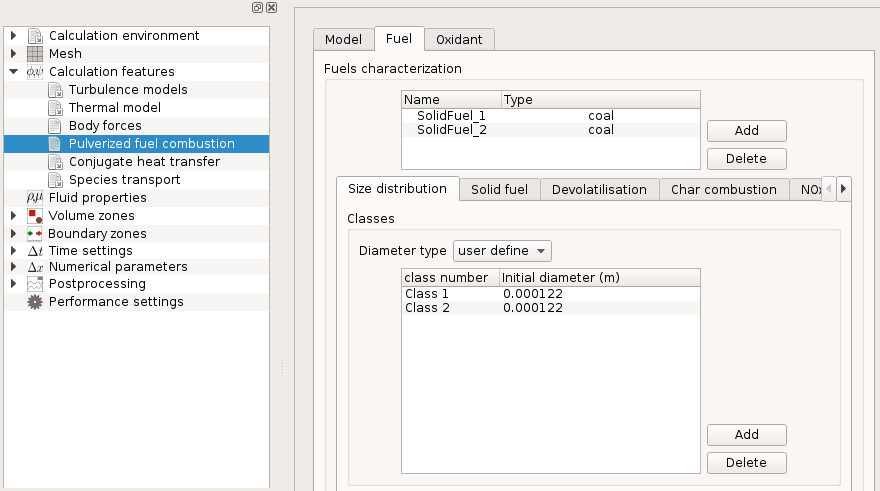
\includegraphics[width=12cm]{gui_coal_classes}
\caption{Thermophysical models - Pulverized coal combustion, coal classes}
\label{fig:Ini-coal1}
\end{center}
\end{figure}

\begin{figure}[!ht]
\begin{center}
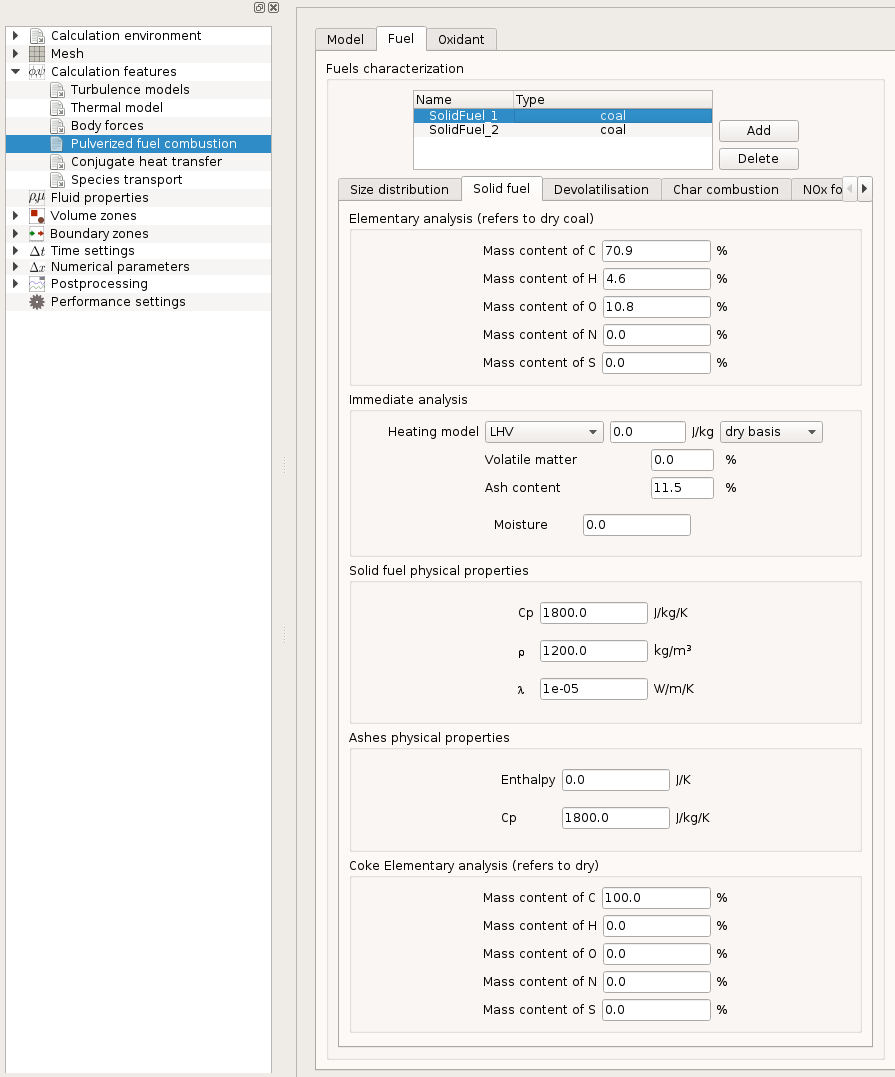
\includegraphics[width=11cm]{gui_coal_composition}
\caption{Pulverized coal combustion, coal composition}
\label{fig:Ini-coal3}
\end{center}
\end{figure}

\begin{figure}[!ht]
\begin{center}
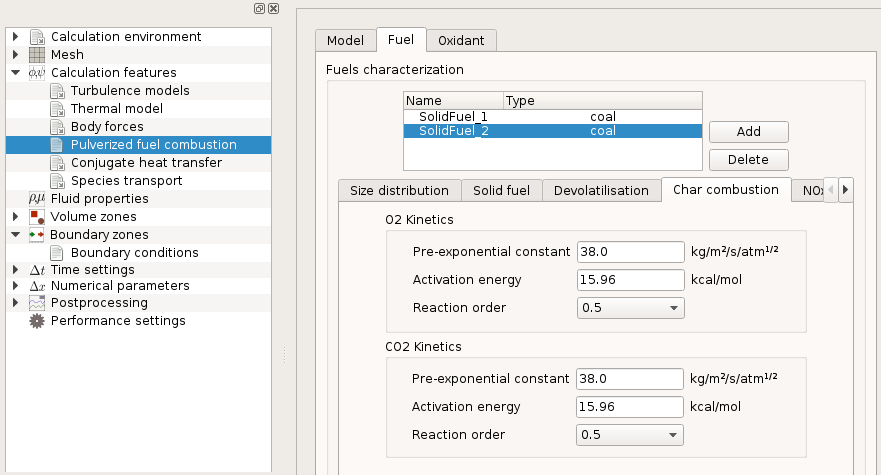
\includegraphics[width=11cm]{gui_coal_reaction}
\caption{Pulverized coal combustion, reaction parameters}
\label{fig:Ini-coal4}
\end{center}
\end{figure}

\begin{figure}[!ht]
\begin{center}
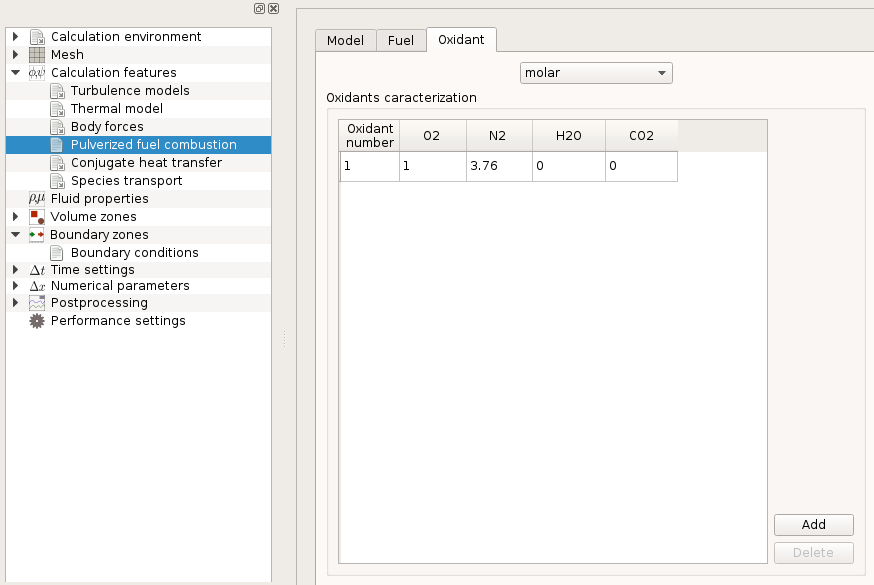
\includegraphics[width=11cm]{gui_coal_oxydant}
\caption{Pulverized coal combustion, oxydant}
\label{fig:Ini-coal5}
\end{center}
\end{figure}

If the user deals with gas combustion or if he (or she) does not want to use the
GUI for coal combustion, the subroutine \texttt{cs\_user\_initialization} must be used (only during the calculation initialisation).\\
In this section, ``specific physics'' will refer to gas combustion or
to pulverised coal combustion.

These subroutines allow the user to initialise some variables specific
to the specific physics activated {\em via} \texttt{usppmo}. As usual,
the user may have access to several geometric variables to discriminate
between different initialisation zones if needed.

It should be recalled again that the user can access the array of values of the
variables as described in the \doxygenfile{field.html}{the \texttt{doxygen}
documentation dedicated to the fields management}. In the following description,
only variables indices \texttt{ivar} are given, but field indices can be
retrieved easily by using \texttt{ivarfl(ivar)}.

{\em WARNING: in the case of a specific physics modelling, all the
variables will be initialised here, even the potential user scalars: {\em
\texttt{cs\_user\_initialization}} is no longer used.}


\begin{list}{$\bullet$}{}
       \item in the case of the EBU pre-mixed flame module, the user can
             initialise in every cell \texttt{iel}: the mixing rate
             \texttt{isca(ifm)} in variable richness, the
             fresh gas mass fraction \\
             \texttt{isca(iygfm\index{iygfm})}
             and the mixture enthalpy \texttt{isca(iscalt)} in
             permeatic conditions

        \item in the case of the rapid complete chemistry diffusion flame
             module, the user can initialise in every cell \texttt{iel}: the
             mixing rate \texttt{isca(ifm\index{ifm})}, its variance
             \texttt{isca(ifp2m\index{ifp2m})} and the mixture mass
             enthalpy \texttt{isca(iscalt)} in permeatic conditions

        \item in the case of the pulverised coal combustion module, the
             user can initialise in every cell \texttt{iel}:
              \begin{list}{$\rightarrow$}{}
                     \item the transport variables related to the solid phase
                           \begin{list}{}{}
                                  \item \texttt{isca(ixch\index{ixch}(icla))}
                                  the reactive coal mass fraction related to the
                                  class \texttt{icla} (\texttt{icla} from 1 to
                                  \texttt{nclacp} which is the total number of
                                  classes, {\em i.e.} for all the coal type)
                                  \item \texttt{isca(ixck(\index{ixck}icla))}
                                  the coke mass fraction related to the class
                                  \texttt{icla}
                                  \item \texttt{isca(inp\index{inp}(icla))} the
                                  number of particles related to class
                                  \texttt{icla} per kg of air-coal mixture
                                  \item \texttt{isca(ih2\index{ih2}(icla))} the
                                   mass enthalpy related to the class
                                   \texttt{icla} in permeatic conditions
                           \end{list}
                     \item \texttt{isca(iscalt)} the mixture enthalpy
                     \item the transport variables related to the gas phase
                           \begin{list}{}{}
                                  \item
                                       \texttt{isca(if1m\index{if1m}(icha))} the
                                       mean value of the tracer 1 representing
                                       the light volatile matters released by
                                       the coal \texttt{icha}
                                  \item
                                       \texttt{isca(if2m\index{if2m}(icha))} the
                                        mean value of the tracer 2 representing
                                        the heavy volatile matters released by
                                        the coal \texttt{icha}
                                  \item \texttt{isca(if3m\index{if3m})}
                                        the mean value of the tracer 3
                                        representing the carbon released
                                        as CO during coke burnout
                                  \item \texttt{isca(if4p2m\index{if4p2m})} the
                                  variance associated with the tracer 4
                                  representing the air (the mean value of this
                                  tracer is not transported, it can be deduced
                                  directly from the three others)
                                  \item \texttt{isca(ifp3m\index{ifp3m})} the
                                  variance associated with the tracer 3
                           \end{list}
              \end{list}
\end{list}

%==================================
\subsubsection{Boundary conditions}\label{sec:coal-cl}
%==================================
In this section, ``specific physics'' refers to gas combustion or
to pulverised coal combustion.\\
For coal combustion, it is possible to manage the boundary conditions in the Graphical User Interface (GUI). When the coal combustion physics is selected in the heading ``Thermophysical models'', specific boundary conditions are activated for inlets, see \figurename~\ref{fig:cond_lim-coal}. The user fills for each type of coal previously defined (see \S~\ref{sec:Ini-coal}) the initial temperature and initial composition of the inlet flow, as well as the mass flow rate.

\begin{figure}[!ht]
\begin{center}
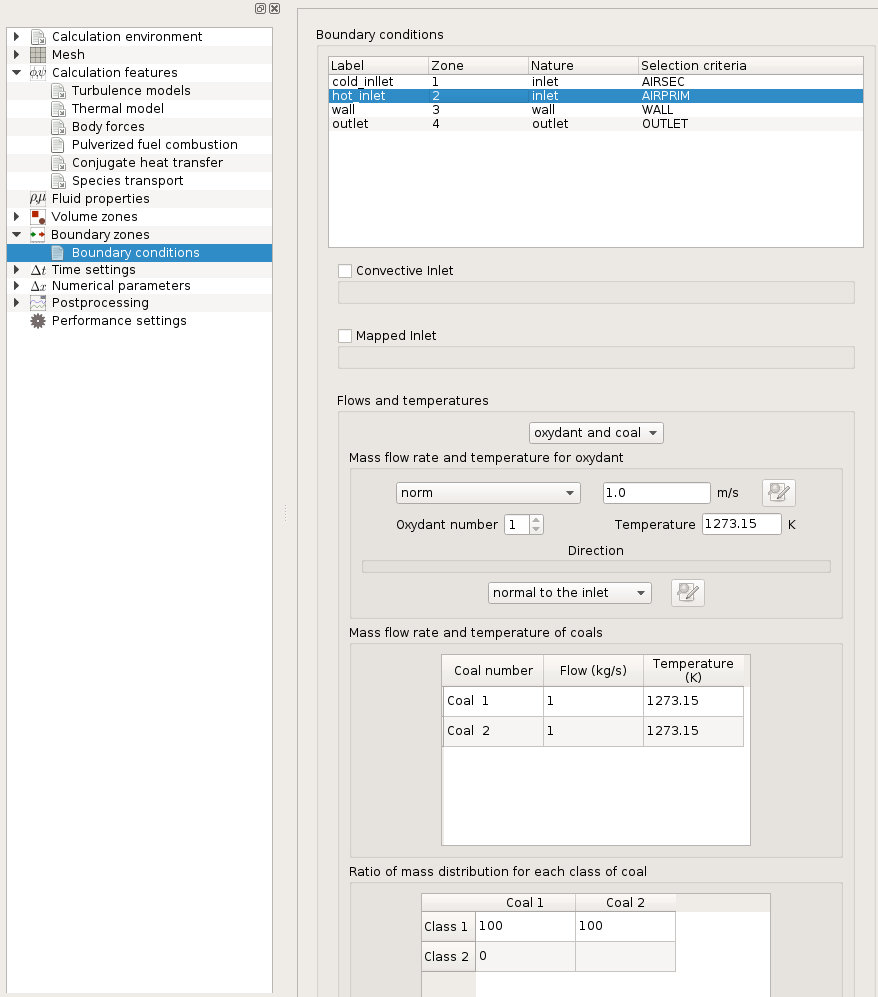
\includegraphics[width=13cm]{gui_coal_bc}
\caption{Boundary conditions for the combustion of coal}
\label{fig:cond_lim-coal}
\end{center}
\end{figure}

For gas combustion or if the GUI is not used for coal combustion, the use of
\texttt{cs\_user\_boundary\_conditions} (called at every time step) is as
mandatory as \texttt{cs\_user\_parameters.f90} and \texttt{usppmo} to run a calculation involving specific physics. The way of using them is the same as using
 in the framework of standard calculations, that is, run several loops on the boundary faces lists (cf. \S\ref{sec:fvm_selector})
marked out by their colors, groups, or  geometrical criterion, where
the type of face, the type of boundary condition for each variable and
eventually the value of each variable are defined.

{\em WARNING: In the case of a specific physics modelling, all the
boundary conditions for every variable must be defined here, even for
the eventual user scalars: {\em \texttt{cs\_user\_boundary\_conditions}} is not used at all.}\\

In the case of a specific physics modelling, a zone number \texttt{izone}
\footnote{\texttt{izone} must be less than the maximum number of boundary
zone allowable by the code, \texttt{nozppm}. This is fixed at 2000 in
 \texttt{pppvar};not to be modified} (for
instance the color \texttt{icoul}) is associated with every boundary face, in
order to gather together all the boundary faces of the same type. In
comparison to \texttt{cs\_user\_boundary\_conditions}, the main change from the user point of
view concerns the faces whose boundary conditions belong to the type
\texttt{itypfb=ientre\index{ientre}}:

\begin{list}{$\bullet$}{}
       \item for the EBU pre-mixed flame module:
             \begin{list}{$\rightarrow$}{}
                    \item the user can choose between the ``burned gas
                          inlet'' type (marked out by the burned gas indicator
                          \texttt{ientgb\index{ientgb}(izone\index{izone})}=1) and the
                          ``fresh gas inlet'' type (marked out by
                          the fresh gas indicator
                          \texttt{ientgf\index{ientgf}(izone)}=1)
                    \item for each inlet type (fresh or burned
                          gas), a mass flow or a velocity must be imposed:

                          \begin{list}{-}{}
                                 \item to impose the mass flow,
                                     \begin{list}{-}{}
                                       \item the user gives to
                                             the indicator
                                             \texttt{iqimp\index{iqimp}(izone)}
                                             the value 1,
                                       \item  the
                                             mass flow value is set in
                                             \texttt{qimp\index{qimp}(izone)}
                                             (positive value, in $kgs^{-1}$)
                                       \item finally he imposes the
                                             velocity vector direction
                                             by giving the components of
                                             a direction vector in
                                             \texttt{rcodcl\index{rcodcl}(ifac,iu\index{iu})}, \texttt{rcodcl(ifac,iv\index{iv})} and \texttt{rcodcl(ifac,iw\index{iw})}
                                     \end{list}

{\em WARNING:
\begin{list}{-}{}
\item the variable \texttt{qimp(izone)} refers to the mass flow across the whole
      zone \texttt{izone} and not across a boundary face (specifically for the axi-symmetric calculations, the inlet surface of the mesh must be broken up)
\item the variable \texttt{qimp(izone)} deals with the inflow across the area \texttt{izoz} and only across this zone; it is recommended to pay attention to the boundary conditions.
\item the velocity direction vector is neither necessarily normed, nor
      necessarily incoming.
\end{list}}

                                 \item to impose a velocity, the user
                                       must give to the indicator
                                       \texttt{iqimp(izone)} the value 0 and set
                                       the three velocity components (in
                                       $m.s^{-1}$) in
                                       \texttt{rcodcl(ifac,iu)},
                                       \texttt{rcodcl(ifac,iv)} and
                                       \texttt{rcodcl(ifac,iw)}
                          \end{list}
                    \item finally he specifies for each gas inlet type
                          the mixing rate \texttt{fment\index{fment}(izone)} and
                          the temperature \texttt{tkent\index{tkent}(izone)} in Kelvin
             \end{list}

       \item for the ``3 points'' diffusion flame module:
             \begin{list}{$\rightarrow$}{}
                    \item the user can choose between the ``oxidiser
                          inlet'' type marked out by
                          \texttt{ientox\index{ientox}(izone)}=1 and the ``fuel
                          inlet'' type marked out by
                          \texttt{ientfu\index{ientfu}(izone)}=1
                    \item concerning the input mass flow or the input
                          velocity, the method is the same as for the
                          EBU pre-mixed flame module
                    \item finally, the user sets the temperatures
                          \texttt{tinoxy\index{tinoxy}} for each oxidiser inlet
                          and \texttt{tinfue\index{tinfue}}, for each fuel inlet

{\em Note: In the standard version, only the cases with only one
                          oxidising inlet type and one fuel inlet type
                          can be treated. In particular, there must be
                          only one input temperature for the oxidiser
                          (\texttt{tinoxy}) and one input temperature for the
                          fuel (\texttt{tinfuel}).}
             \end{list}

       \item for the pulverised coal module:
             \begin{list}{$\rightarrow$}{}
                    \item the inlet faces can belong to the ``primary
                          air and pulverised coal inlet'' type, marked
                          out by \texttt{ientcp\index{ientcp}(izone)}=1, or to
                          the ``secondary or tertiary air inlet'' type,
                          marked out by \texttt{ientat\index{ientat}(izone)}=1
                    \item in a way which is similar to the process
                          described in the framework of the EBU module,
                          the user chooses for every inlet face to
                          impose the mass flow or not (\texttt{iqimp(izone)}=1 or
                          0). If the mass flow is imposed, the user
                          must set the air mass flow value
                          \texttt{qimpat\index{qimpat}(izone)}, its direction in
                          \texttt{rcodcl(ifac,iu)}, \texttt{rcodcl(ifac,iv)}
                          and \\ \texttt{rcodcl(ifac,iw)} and if
                    \item incoming air temperature \texttt{timpat\index{timpat}(izone)} in
                          Kelvin. If the velocity is imposed, he must
                          set  \texttt{rcodcl(ifac,iu)}, \\
                          \texttt{rcodcl(ifac,iv)} and \texttt{rcodcl(ifac,iw)}.

                    \item if the inlet belongs to the ``primary air and
                          pluverised coal'' \texttt{type (ientcp(izone) = 1)} the
                          user must also define for each coal type \texttt{icha}:
                          the mass flow
                          \texttt{qimpcp\index{qimpcp}(izone,icha)}, the
                          granulometric distribution
                          \texttt{distch\index{distch}(izone,icha,iclapc)}
                          related to each class \texttt{iclacp}, and the
                          injection temperature
                          \texttt{timpcp\index{timpcp}(izone,icha)}

             \end{list}
\end{list}

%==================================
\subsubsection{Initialisation of the options of the variables}
%==================================
In the case of coal combustion, time averages, chronological records and logss follow-ups can be set in the Graphical User Interface (GUI) or in the subroutines \texttt{cs\_user\_combustion}. In the GUI, under the heading ``Calculation control'', additional variables appear in the list in the items ``Time averages'' and ``Profiles'', as well as in the item Volume solution control'', see \figurename~\ref{fig:t_average-coal} and \figurename~\ref{fig:V_control-coal}.

\begin{figure}[!ht]
\begin{center}
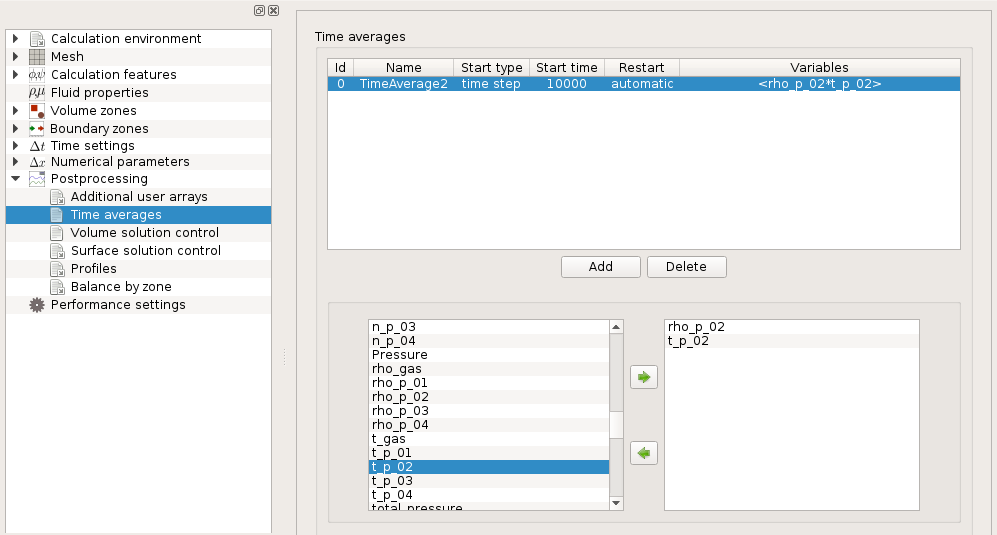
\includegraphics[width=12cm]{gui_coal_time_average}
\caption{Calculation control - Time averages}
\label{fig:t_average-coal}
\end{center}
\end{figure}

\begin{figure}[!ht]
\begin{center}
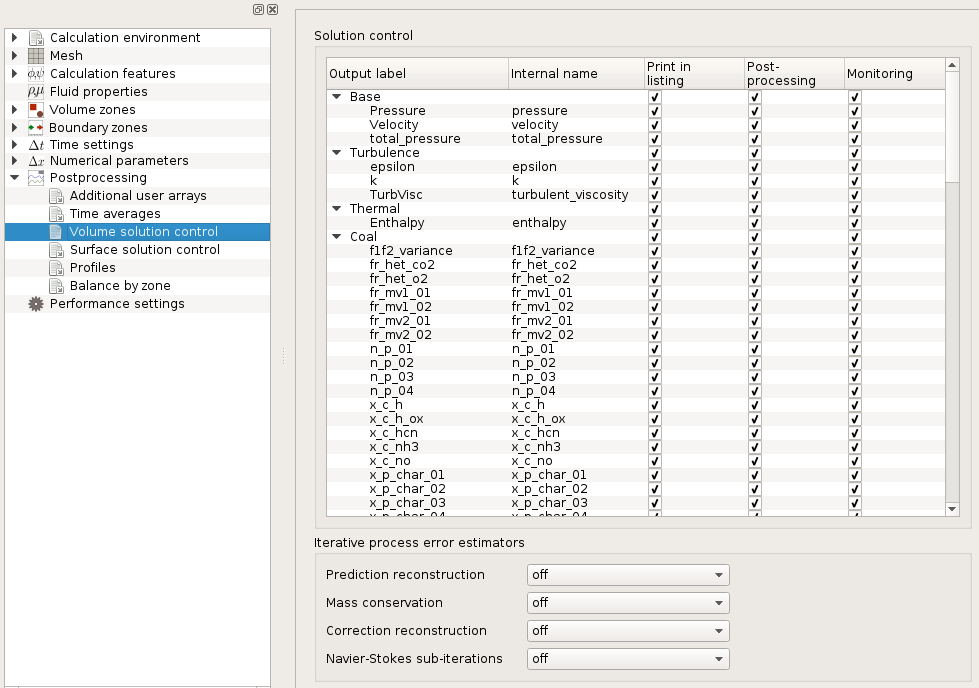
\includegraphics[width=13cm]{gui_coal_solution_control}
\caption{Calculation control - Volume solution control}
\label{fig:V_control-coal}
\end{center}
\end{figure}

In this section, ``specific physics'' refers to gas combustion or
pulverised coal combustion.

For gas combustion or if the GUI is not used for coal combustion, the 3
subroutines \texttt{cs\_user\_combustion} can be used to complete
\texttt{cs\_user\_parameters.f90} for the considered specific physics. These
subroutines are called at the calculation start.
They allow to:
\begin{list}{$\bullet$}{}
\item activate, for the variables which are specific to the activated specific
      physics module, chronological records at the probes defined in
      \texttt{cs\_user\_parameters.f90}.\\
      Concerning the main variables (velocity, pressure, etc ...) the user
      must still complete \texttt{cs\_user\_parameters.f90} if he wants to get
      chronological records, printings in the log or chronological
      outputs.
      The variables which can be activated by the user for each specific
      physics are listed below. The solved variables (of variable indices
      \texttt{ivar}) and the properties of indices \texttt{iprop} (defined at
      the cell \texttt{iel} by \texttt{cpro\_prop(iel)} which is obtained
      by calling \texttt{field\_get\_val\_s(iprop, cpro\_prop)})
      are listed below:
      \begin{list}{$\rightarrow$}{}
       \item EBU pre-mixed flame modelling:
       \begin{list}{-}{}
        \item Solved variables
              \begin{list}{\texttt{ivar} = }{}
               \item \texttt{isca(iygfm\index{iygfm})} fresh gas mass fraction
               \item \texttt{isca(ifm\index{ifm})} mixing rate
               \item \texttt{isca(ihm\index{ihm})} enthalpy, if transported
              \end{list}
        \item Properties \texttt{cpro\_prop(iel)}
              \begin{list}{\texttt{iprop} = }{}
               \item \texttt{itemp\index{itemp}} temperature
               \item \texttt{iym(1)\index{iym(1)}} fuel mass fraction
               \item \texttt{iym(2)\index{iym(2)}} oxidiser mass fraction
               \item \texttt{iym(3)\index{iym(3)}} product mass fraction
               \item \texttt{ickabs\index{ickabs}} absorption
                     coefficient, when the radiation modelling is
                     activated
               \item \texttt{it3m\index{it3m}} and \texttt{it4m\index{it4m}}
                     ``$T^3$'' and ``$T^4$'' terms, when the radiation
                     modelling is activated
              \end{list}
       \end{list}
       \item rapid complete chemistry diffusion flame modelling:
             \begin{list}{}{}
              \item  everything is identical to the ``EBU'' case, except
                     the fresh gas mass fraction which is replaced by the
                     variance of the mixing rate
                     \texttt{ivar=isca(ifp2m\index{ifp2m})}
             \end{list}
       \item pulverised coal modelling with 3 combustibles:
             \begin{list}{}{}
              \item {\em variables shared by the two phases}:
                    \begin{list}{-}{}
                     \item Solved variables
                           \begin{list}{\texttt{ivar} = }{}
                            \item \texttt{isca(ihm\index{ihm})}: gas-coal
                                  mixture enthalpy
                            \item \texttt{isca(immel\index{immel})}: molar mass
                                  of the gas mixture
                           \end{list}
                    \end{list}
              \item {\em variables specific to the dispersed phase}:
              \begin{list}{-}{}
               \item Solved variables
                     \begin{list}{\texttt{ivar} = }{}
                      \item \texttt{isca(ixck\index{ixck}(icla))}: coke mass
                            fraction related to the class \texttt{icla}
                      \item \texttt{isca(ixch\index{ixch}(icla))}: reactive coal
                            mass fraction related to the class \texttt{icla}
                      \item \texttt{isca(inp\index{inp}(icla))}: number of
                            particles of the class \texttt{icla} per kg of
                            air-coal mixture
                      \item \texttt{isca(ih2\index{ih2}(icla))}: mass enthalpy
                            of the coal of class \texttt{icla}, if we are in
                            permeatic conditions
                     \end{list}
               \item Properties \texttt{cpro\_prop(iel)}
                     \begin{list}{\texttt{iprop} = }{}
                      \item \texttt{immel\index{immel}}: molar mass of the gas
                            mixture
                      \item \texttt{itemp2\index{itemp2}(icla)}: temperature of
                            the particles of the class \texttt{icla}
                      \item \texttt{irom2\index{irom2}(icla)}: density of
                            the particles of the class \texttt{icla}
                      \item \texttt{idiam2\index{idiam2}(icla)}: diameter of the
                            particles of the class \texttt{icla}
                      \item \texttt{igmdch\index{igmdch}(icla)}: disappearance
                            rate of the reactive coal of the class \texttt{icla}
                      \item \texttt{igmdv1\index{igmdv1}(icla)}: mass transfer
                            caused by the release of light volatiles
                            from the class \texttt{icla}
                      \item \texttt{igmdv2\index{igmdv2}(icla)}: mass transfer
                            caused by the release of heavy volatiles
                            from the class \texttt{icla}
                      \item \texttt{igmhet\index{igmhet}(icla)}: coke
                            disappearance rate during the coke burnout
                            of the class \texttt{icla}
                      \item \texttt{ix2\index{ix2}(icla)}: solid mass fraction
                            of the class \texttt{icla}
                     \end{list}
              \end{list}
              \item {\em variables specific to the continuous phase}:
              \begin{list}{-}{}
               \item Solved variables
                     \begin{list}{\texttt{ivar} = }{}
                      \item \texttt{isca(if1m\index{if1m}(icha))}: mean value of
                            the tracer 1 representing the light
                            volatiles released by the coal \texttt{icha}
                      \item \texttt{isca(if2m\index{if2m}(icha))}: mean value of
                            the tracer 2 representing the heavy
                            volatiles released by the coal \texttt{icha}
                      \item \texttt{isca(if3m)\index{if3m}}: mean value of the
                            tracer 3 representing the carbon released as
                            CO during coke burnout
                      \item \texttt{isca(if4pm\index{if4pm})}: variance of the
                            tracer 4 representing the air
                      \item \texttt{isca(if3p2m\index{if3p2m})}: variance of the
                            tracer 3
                     \end{list}
               \item Properties \texttt{cpro\_prop(iel)}
                     \begin{list}{\texttt{iprop} = }{}
                      \item \texttt{itemp1\index{itemp1}}: temperature of the
                            gas mixture
                      \item \texttt{iym1(1)\index{iym1(1)}}: mass fraction of
                            $CH_{X1m}$ (light volatiles) in the gas
                            mixture
                      \item \texttt{iym1(2)\index{iym1(2)}}: mass fraction of
                            $CH_{X2m}$ (heavy volatiles) in the gas
                            mixture
                      \item \texttt{iym1(3)\index{iym1(3)}}: mass fraction of
                            CO in the gas mixture
                      \item \texttt{iym1(4)\index{iym1(4)}}: mass fraction of
                            $O_2$ in the gas mixture
                      \item \texttt{iym1(5)\index{iym1(5)}}: mass fraction of
                            $CO_2$ in the gas mixture
                      \item \texttt{iym1(6)\index{iym1(6)}}: mass fraction of
                            $H_2O$ in the gas mixture
                      \item \texttt{iym1(7)\index{iym1(7)}}: mass fraction of
                            $N_2$ in the gas mixture
                     \end{list}
              \end{list}
             \end{list}
      \end{list}

 \item set the relaxation coefficient of the density \texttt{srrom}, with \\
$\rho^{n+1}=\texttt{srrom}*\rho^{n}+(1-\texttt{srrom})\rho^{n+1}$\\
(the default value is \texttt{srrom\index{srrom}} = 0.8. At the
      beginning of a calculation, a sub-relaxation of 0.95 may reduce
      the numerical ``shocks'').

 \item set the dynamic viscosity \texttt{diftl0}. By default
      \texttt{diftl0\index{diftl0}}= 4.25 $kgm^{-1}s^{-1}$
(the dynamic diffusivity being the ratio between the thermal
      conductivity $\lambda$ and the mixture specific heat $C_p$ in the
      equation of enthalpy).

 \item set the value of the constant \texttt{cebu\index{cebu}} of the Eddy Break
      Up model (only in \texttt{cs\_user\_combustion}. By default \texttt{cebu}=2.5)
\end{list}

%==================================
\subsection{Heavy fuel oil combustion module}
%==================================
%==================================
\subsubsection{Initialisation of transported variables}
%==================================
To initialise or modify (in case of a continuation) values of transported
variables and of the time step, the standard subroutine \texttt{cs\_user\_initialization} is used.

Physical properties are stored using the \texttt{cs\_field} API (cell center). For instance, to obtain \texttt{rom(iel)},
the mean density (in $kg.m^{-3}$), one must declare a \texttt{ncelet} array \texttt{cpro\_rom} and then call
\texttt{call field\_get\_val\_s(icrom, cpro\_rom)}.\\
Physical properties (\texttt{rom, viscl, cp, ...}) are computed in \texttt{ppphyv} and are not to be modified here.

The \texttt{cs\_user\_initialization-fuel.f90} example illustrates how the user
may initialise quantities related to gaseous species and droplets compositions
in addition to the chosen turbulent model.

%==================================
\subsubsection{Boundary conditions}
%==================================
Boundary conditions are defined as usual on a per-face basis in
\texttt{cs\_user\_boundary\_conditions}. They may be assigned in two ways:
\begin{list}{.}{}
\item for ``standard'' boundary conditions (inlet, free outlet, wall, symmetry): a code is defined in the array \texttt{itypfb} (of dimensions equal to the number of boundary faces). This code will then be used by a non-user subroutine to assign the conditions.
\item for ``non-standard'' conditions: see details given in
  \texttt{cs\_user\_boundary\_conditions-fuel.f90} example.
\end{list}

%==================================
\subsection{Radiative thermal transfers in semi-transparent gray media}
%==================================
%==================================
\subsubsection{Initialisation of the radiation main parameters}
%==================================

The main radiation parameters can be initialise in the Graphical User Interface (GUI) or in the user subroutine \texttt{cs\_user\_radiative\_transfer\_param}. In the GUI, under the heading ``Thermophysical models'', when one of the two thermal radiative transfers models is selected, see \figurename~\ref{fig:0_ray}, additional items appear. The user is asked to choose the number of directions for angular discretisation, to define the absorption coefficient and select if the radiative calculation are restarted or not,
see \figurename~\ref{fig:1_ray} and \figurename~\ref{fig:3_ray}. When ``Advanced options'' is selected for both models \figurename~\ref{fig:2_ray} or \figurename~\ref{fig:4_ray} appear, the user must fill the resolution frequency and verbosity levels. In addition, the activation of the radiative transfer leads to the creation of an item ``Surface solution control'' under the heading ``Calculation control'',
see \figurename~\ref{fig:5_ray}, where radiative transfer variables can be selected to appear in the output log.

\begin{figure}[ht]
\begin{center}
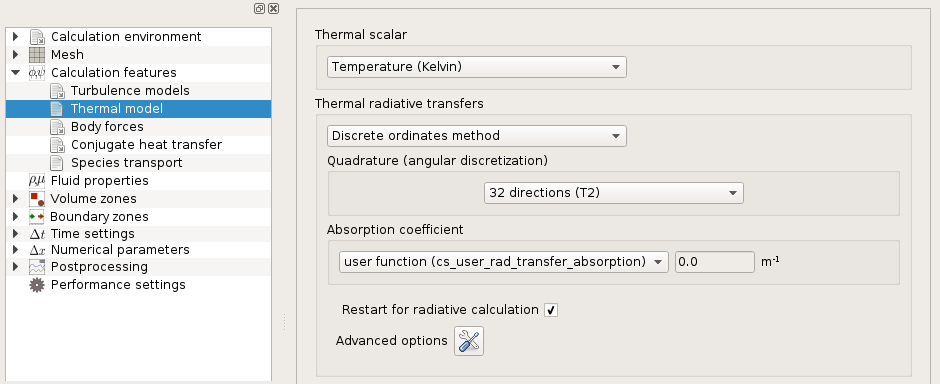
\includegraphics[width=0.9\textwidth]{gui_rad_transf_do_params}
\caption{Radiative transfers - parameters of the DO method}
\label{fig:1_ray}
\end{center}
\end{figure}

\begin{figure}[ht]
\begin{center}
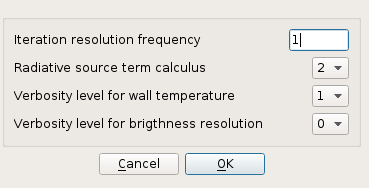
\includegraphics[width=7cm]{gui_rad_transf_do_advanced}
\caption{Radiative transfers - advanced parameters of the DO method}
\label{fig:2_ray}
\end{center}
\end{figure}

\begin{figure}[ht]
\begin{center}
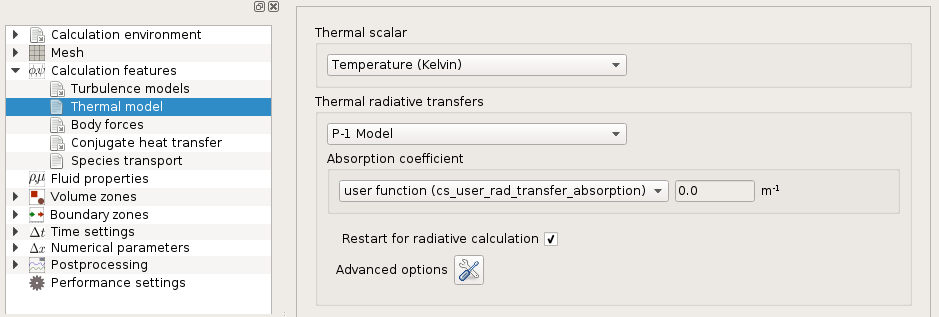
\includegraphics[width=0.9\textwidth]{gui_rad_transf_p1_params}
\caption{Radiative transfers - parameters of the P-1 model}
\label{fig:3_ray}
\end{center}
\end{figure}

\begin{figure}[ht]
\begin{center}
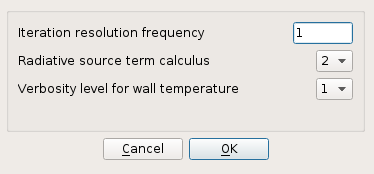
\includegraphics[width=7cm]{gui_rad_transf_p1_advanced}
\caption{Radiative transfers - advanced parameters of the P-1 model}
\label{fig:4_ray}
\end{center}
\end{figure}

\begin{figure}[ht]
\begin{center}
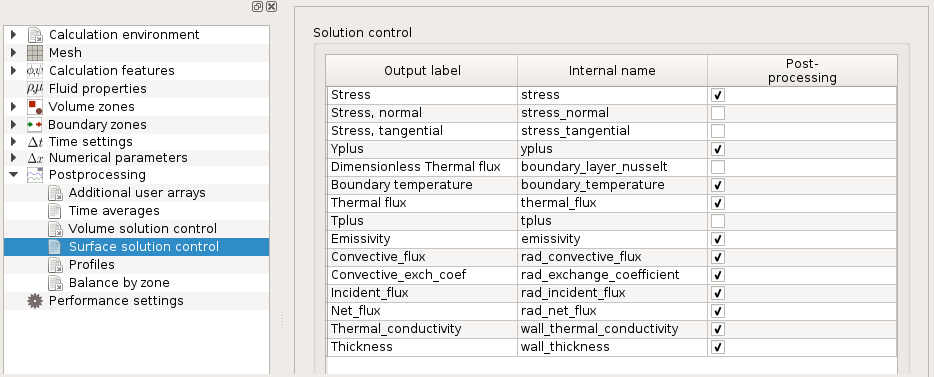
\includegraphics[width=0.9\textwidth]{gui_rad_transf_post_output}
\caption{Calculation control - Radiative transfers post-processing output}
\label{fig:5_ray}
\end{center}
\end{figure}

If the GUI is not used, \texttt{cs\_user\_radiative\_transfer\_param} is one of the two subroutine which must be completed by the user for all
calculations including radiative thermal transfers. It is called only during the calculation initialisation. It is composed of three headings. The first one is dedicated to the activation
of the radiation module, only in the case of classic physics. \\
{\em WARNING: when a calculation is ran using a specific physics module,
this first heading must not be completed. The radiation module is then
activated or not, according to the parameter file related to the considered
specific physics.} \\

\noindent
In the second heading the basic parameters of the radiation module are indicated.\\
Finally, the third heading deals with the selection of the
post-processing graphic outputs. The variables to treat are splitted
into two categories: the volumetric variables and those related to the
boundary faces.\\

\noindent
For more details about the different parameters, the user may refer to the
keyword list (\S~\ref{sec:prg_motscles}).


%==================================
\subsubsection{Radiative transfers boundary conditions}
%==================================
These informations can be filled by the user through the Graphical User Interface
(GUI) or by using the subroutine \texttt{cs\_user\_radiative\_transfer\_bcs.c} (called every time step). If the
interface is used, when one of the ``Radiative transfers'' options is selected in
\figurename~\ref{fig:gui_thermal_scalar}, it activates specific boundary conditions each time
a ``Wall'' is defined, see \figurename~\ref{fig:6_ray}. The user can then choose
between 3 cases. The parameters the user must specify are displayed for one of
them in \figurename~\ref{fig:7_ray}.

\begin{figure}[ht]
\begin{center}
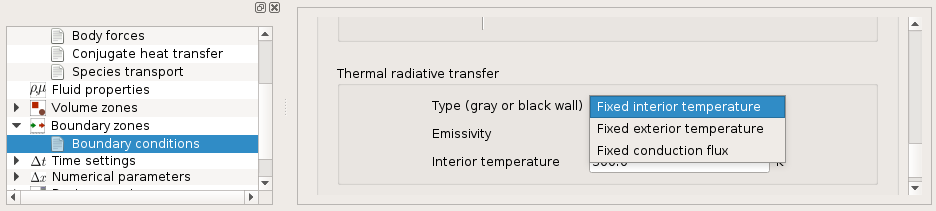
\includegraphics[width=0.9\textwidth]{gui_rad_transf_wall_model}
\caption{Boundary conditions - choice of wall thermal radiative transfers}
\label{fig:6_ray}
\end{center}
\end{figure}

\begin{figure}[ht]
\begin{center}
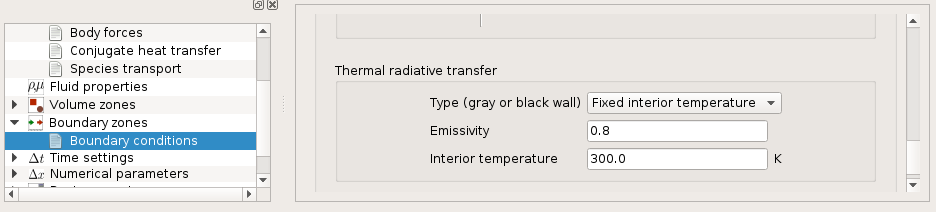
\includegraphics[width=0.9\textwidth]{gui_rad_transf_wall_params}
\caption{Boundary conditions - example of wall thermal radiative transfer}
\label{fig:7_ray}
\end{center}
\end{figure}

When the GUI is not used, \texttt{cs\_user\_radiative\_transfer\_bcs.f90} is the second subroutine necessary for
every calculation which includes radiative thermal transfers. It is used to give all the
necessary parameters concerning, in the one case, the wall temperature
calculation, and in the other, the coupling between the thermal
scalar (temperature or enthalpy), and the radiation module at the
calculation domain boundaries. It must be noted that the boundary conditions
concerning the thermal scalar which may have been defined in the
subroutine \texttt{cs\_user\_boundary\_conditions} will be modified by the radiation module
according to the data given in \texttt{cs\_user\_radiative\_transfer\_bcs.f90} (cf. \S\ref{sec:fvm_selector}).\\
A zone number must be given to each boundary face \footnote{This must be less
 than the maximum allowable by the code, \texttt{nozrdm}. This is fixed at 2000
 in \texttt{radiat} and cannot be modified.} and, specifically for
the walls, a boundary condition type and an initialisation temperature
(in Kelvin). The initialisation temperature is only used to make the
solving implicit at the first time step. The zone number allows assigning
an arbitrary integer to a set of boundary faces having the same
radiation boundary condition type. This gathering is used by the
calculation, and in the log to print some physical values (mean
temperature, net radiative flux ...). An independent graphic output in
{\em EnSight} format is associated with each zone and allows the display on
the boundary faces of the variables selected in the third heading of the
subroutine \texttt{cs\_user\_radiative\_transfer\_param}.\\
A boundary condition type stored in the array ISOTHP is associated with
each boundary face. There are five different types:

\begin{list}{$\bullet$}{}

\item \texttt{\textbf{itpimp}}: wall face with imposed temperature,

\item \texttt{\textbf{ipgrno}}: for a grey or black wall face, calculation of the
      temperature by means of a flux balance,

\item \texttt{\textbf{iprefl}}: for a reflecting wall face, calculation of the
      temperature by means of a flux balance.
 This is fixed at 2000 in \texttt{radiat} and cannot be modified.

\item \texttt{\textbf{ifgrno}}: grey or black wall face to which a conduction
      flux is imposed,

\item \texttt{\textbf{ifrefl}}: reflecting wall face to which a conduction
      flux is imposed, which is equivalent to impose this flux directly
      to the fluid.

\item \texttt{\textbf{ifinfe}}: for an open boundary (inlet or outlet) or symmetry face,
      simulate an infinite extrusion by applying a Neumann condition to
      the radiation equations,

\end{list}

\noindent
Depending on the selected boundary condition type at every wall face,
the code needs to be given some additional information:

\begin{list}{$\bullet$}{}

\item \texttt{\textbf{itpimp}}: the array \texttt{tintp} must be completed
      with the imposed temperature value and the array \texttt{epsp} must
      be completed with the emissivity value (strictly positive).

\item \texttt{\textbf{ipgrno}}: must be given: an initialisation temperature in
      the array \texttt{tintp}, the wall emissivity (strictly positive, in
      \texttt{epsp}), thickness (in \texttt{epap}), thermal conductivity
      (in \texttt{xlamp}) and an external temperature (in \texttt{textp})
      in order to calculate a conduction flux across the wall.

\item \texttt{\textbf{iprefl}}: must be given: an initialisation temperature (in
      \texttt{tintp}), the wall thickness (in \texttt{epap}) and thermal conductivity (in
      \texttt{xlamp}) and an external temperature (in \texttt{textp}).

\item \texttt{\textbf{ifgrno}}: must be given: an initialisation temperature (in
      \texttt{tintp}), the wall emissivity (in \texttt{epsp}) and the conduction
      flux (in $W/m^2$ whatever the thermal scalar, enthalpy or temperature) in
      the array \texttt{rcodcl}. The value of \texttt{rcodcl} is positive when the
      conduction flux is directed from the inside of the fluid domain to the
      outside (for instance, when the fluid heats the walls). If the
      conduction flux is null, the wall is adiabatic.

\item \texttt{\textbf{ifrefl}}: must be given: an initialisation temperature (in
      \texttt{tintp}) and the conduction flux (in $W/m^2$ whatever the thermal
      scalar) in the array \texttt{rcodcl}. The value of \texttt{rcodcl} is
      positive when the conduction flux is directed from the inside of the
      fluid domain to the outside (for instance, when the fluid heats the
      walls). If the conduction flux is null, the wall is adiabatic. The flux
      received by \texttt{rcodcl} is directly imposed as boundary condition for
      the fluid.

\end{list}

\noindent
{\em WARNING: it is mandatory to set a zone number to every boundary
face, even those which are not wall faces. These zones will be used during the
printing in the log. It is recommended to gather together the
boundary faces of the same type, in order to ease the reading of
run\_solver.log.}\\

%==================================
\subsubsection{Absorption coefficient of the medium, boundary conditions
   for the luminance and calculation of the net radiative flux}
%==================================

When the absorption coefficient is not constant, the subroutine
\texttt{cs\_user\_rad\_transfer\_absorption} is called instead at each time
step. It is composed of three parts. In the first one, the user
must provide the absorption coefficient of the medium in the array CK,
for each cell of the fluid mesh. By default, the absorption coefficient
of the medium is 0, which corresponds to a transparent medium.\\

{\em WARNING: when a specific physics is activated, it is forbidden to
give a value to the absorption coefficient in this subroutine. In this
case, the coefficient is either calculated automatically, or provided by the user {\em via} a
thermo-chemical parameter file (dp\_C3P or dp\_C3PSJ for gas combustion,
and dp\_FCP for pulverised coal combustion).}\\

\noindent
The two following parts of this subroutine concern a more advanced use
of the radiation module. It is about imposing boundary conditions to the
equation of radiative transfer and net radiative flux calculation, in
coherence with the luminance at the boundary faces, when the user wants
to give it a particular value. In most cases, the given examples do not
need to be modified.

%==================================
\subsection{Conjugate heat transfer}
%==================================

%========================================
\subsubsection{Thermal module in a 1D wall}
%========================================

\noindent
\textit{subroutine called at every time step}

This subroutine takes into account the wall-affected thermal inertia.
 Some boundary faces are treated as a solid wall with a given thickness, on
 which the code resolves a one-dimensional equation for the heat conduction.
 The coupling between the 1D module and the fluid works in a similar way to
 the coupling with the \syrthes. By construction, the user is not able to
 account for the heat transfer between different parts of the wall. A physical
 analysis of each problem, case by case is required in order to evaluate the relevance
 of its usage by way of a report of the simple conditions (temperature, zero-flux
 ) or a coupling with \syrthes.\\

The use of this code requires that the thermal scalar is
defined as (\texttt{iscalt}$>0$).

{\em WARNING: The 1D thermal module is developed assuming the thermal scalar
 as a temperature. If the thermal scalar is an enthalpy, the code calls the
 subroutine \texttt{usthht} for each transfer of data between the fluid
 and the wall in order to convert the enthalpy to temperature and vice-versa.
 This function has not been tested and is firmly discouraged. If the thermal
 variable is the total (compressible) energy, the thermal module will not work.}

%==================================
\subsubsection{Fluid-Thermal coupling with \syrthes}
%==================================
When the user wishes to couple \CS with \syrthes to include heat transfers, he can do so with using with the Graphical User Interface (GUI) or the
\texttt{cs\_syrthes\_coupling} user function.
To set such a coupling in the Graphic User Interfacee (GUI), a thermal scalar must be
selected first in the item ``Thermal scalar'' under the heading ``Thermophysical models''.
Then the item ``Conjugate heat transfer'' will appear, see \figurename\ref{fig:syrthes}.
The zones where the coupling occurs must be defined and a projection axis can be
specified in case of 2D coupling.

\begin{figure}[ht]
\begin{center}
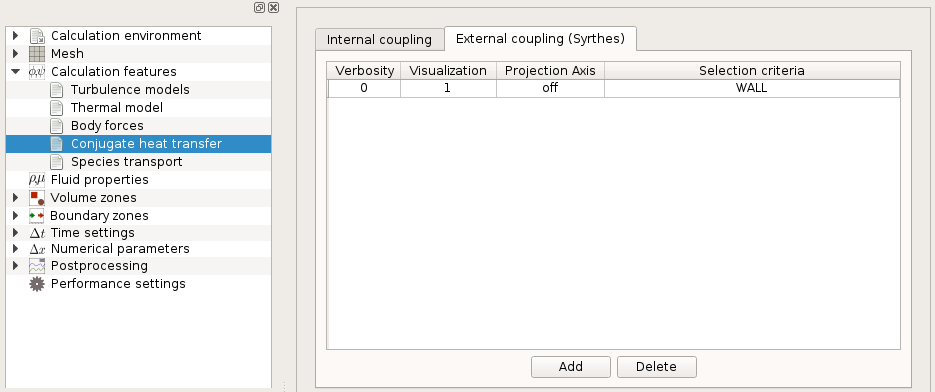
\includegraphics[width=0.9\textwidth]{gui_syrthes_coupling}
\caption{Thermophysical models - coupling with \syrthes}
\label{fig:syrthes}
\end{center}
\end{figure}

If the function \texttt{cs\_user\_syrthes\_coupling} is used, the user must
specify the arguments passed to the '\texttt{cs\_syr\_coupling\_define}' function.
 These arguments are:
\begin{list}{-}{}
 \item \texttt{syrthes\_name} is the matching \syrthes application name (useful only when more than one \syrthes and one \CS domain are present),
 \item \texttt{boundary\_criteria} is the surface selection criteria,
 \item \texttt{volume\_criteria} is the volume selection criteria,
 \item \texttt{projection\_axis}: ' ' if the user wishes to use a 3D standard coupling,
 or specify '$x$', '$y$', or '$z$' as the projection axis if a 2D coupling with \syrthes is used,
 \item \texttt{verbosity} is the verbosity level.
 \item \texttt{visualization} is the visualization level.
\end{list}
Examples are provided in \texttt{cs\_user\_coupling.c}.

The user may also define global coupling options relative to the handling of
time-stepping, by adapting the example \texttt{cs\_user\_coupling}
in the \texttt{cs\_user\_coupling.c} file. In the case of multiple couplings,
these options are global to all \syrthes and \CS couplings.

%==================================
\subsection{Particle-tracking (Lagrangian) Module}
%==================================

%==================================
\subsubsection{General information}\label{sec:over-lag}
%==================================

\begin{itemize}

\item[-] The particle-tracking (or Lagrangian) module enables the simulation of poly-dispersed particulate flows, by calculating the trajectories of individual particles, mainly characterized by their diameter and density (if no heat nor mass transfer between particle and fluid are activated).

\item[-] The standard use of the particle-tracking module follows the \textbf{Moments/PDF approach}: the instantaneous properties of the underlying flow needed to calculate the particle motion are reconstructed from the averaged values (obtained by Reynolds-Averaged Navier-Stokes simulation) by using stochastic processes. The statistics of interest are then obtained through Monte-Carlo simulation.

\item[-] As a consequence, is is important to emphasize that the most important (and physically meaningful) results of a particle-tracking calculation following the Moments/PDF approach are \mbox{\textbf{statistics}}. Volume and surface statistics, steady or unsteady, can be calculated. Individual particle trajectories (as 1D, \textit{EnSight}-readable cases) and displacements (as \textit{EnSight}-readable animations) can also be provided, but only for illustrative purposes.

\end{itemize}

%==================================
\subsubsection{Activating the particle-tracking module}\label{sec:acti-lag}
%==================================

The activation of the particle-tracking module is performed either:
%
\begin{itemize}
 \item [$\bullet$] in the Graphical User Interface (GUI): \texttt{Calculation features} $\rightarrow$ \texttt{Thermophysical models} $\rightarrow$ \texttt{Eulerian-Lagrangian multi-phase treatment}~$\rightarrow$ ~\texttt{particles and droplets tracking}
 \item [$\bullet$] or in the user function \texttt{cs\_user\_lagr\_model}.
\end{itemize}

%==================================
\subsubsection{Basic guidelines for standard simulations}
%==================================

Except for cases in which the flow conditions depend on time, it is generally recommended to perform a first Lagrangian calculation whose aim is to reach a steady-state (i.e. to reach a time starting from which the relevant statistics do not depend on time anymore). In a second step, a calculation restart is done to calculate the statistics. When the single-phase flow is steady and the particle volume fraction is low enough to neglect the particles influence on the continuous phase behaviour, it is recommended to perform a Lagrangian calculation on a frozen field.\\

It is then possible to calculate steady-state volumetric statistics and to give a statistical weight higher than 1 to the particles, in order to reduce the number of simulated (``numerical'') particles to treat while keeping the right concentrations. Otherwise, when the continuous phase flow is steady, but the two-coupling coupling must be taken into consideration, it is still possible to activate steady statistics. \\
When the continuous phase flow is unsteady, it is no longer possible to use steady statistics. To have correct statistics at every moment in the whole calculation domain, it is imperative to have an established particle seeding and it is recommended (when it is possible) not to impose statistical weights different from the unity. \\

Finally, when the so-called complete model is used for turbulent dispersion modelling, the user must make sure that the volumetric statistics are directly used for the calculation of the locally undisturbed fluid flow field.\\

When the thermal evolution of the particles is activated, the associated particulate scalars are always the inclusion temperature and the locally undisturbed fluid flow temperature expressed in degrees Celsius, whatever the thermal scalar associated with the continuous phase is ({\em i.e.} temperature or enthalpy). If the
thermal scalar associated with the continuous phase is the temperature in Kelvin, the unit is converted automatically into Celsius. If the thermal scalar associated with the continuous phase is the enthalpy, the enthalpy-temperature conversion subroutine \texttt{usthht} must be completed for \texttt{mode}=1, and must express temperatures in degrees Celsius. In all cases, the thermal backward coupling of the dispersed phase on the continuous phase is adapted to the thermal scalar transported by the fluid.


%==================================
\subsubsection{Prescribing the main modelling parameters (GUI and/or \texttt{cs\_user\_lagr\_model})}\label{sec:Ini-lag}
%==================================

\minititre{Use of the GUI}

In the GUI, the selection of the Lagrangian module activates the heading \texttt{Particle and droplets tracking} in the tree menu. The initialization is performed in the three items included in this heading:
%
\begin{itemize}
 \item [$\bullet$] \texttt{Global settings}. The user defines in this item the kind of Euler/Lagrange multi-phase treatment, the main parameters, the specific physics associated with the particles and advanced numerical options, see ~\figurename~\ref {fig:Ini-Lag1} to \figurename\ref {fig:Ini-Lag3}.
 \item [$\bullet$] \texttt{Statistics}. The user can select the volume and boundary statistics to be post-processed.
 \item [$\bullet$] \texttt{Output}. The user defines the output frequency and post-processing options for particles and select the variables that will appear in the log.
\end{itemize}

\begin{figure}[ht]
\begin{center}
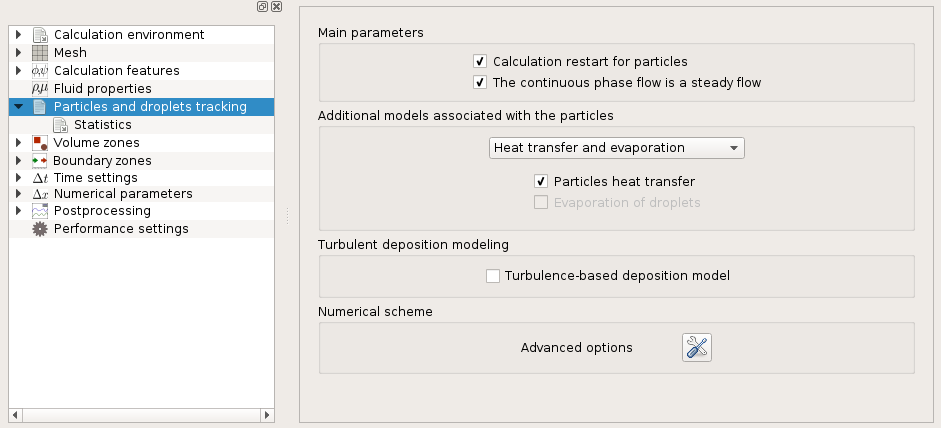
\includegraphics[width=0.9\textwidth]{gui_lagr_global_settings}
\caption{Lagrangian module - View of the \texttt{Global Settings} page}
\label{fig:Ini-Lag1}
\end{center}
\end{figure}
%
 \begin{figure}[ht]
 \begin{center}
 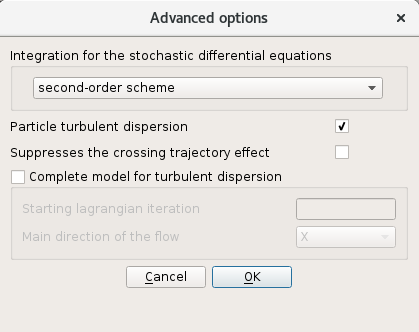
\includegraphics[width=8cm]{gui_lagr_global_advanced}
 \caption{Lagrangian module - Global Settings, advanced numerical options}
 \label{fig:Ini-Lag3}
 \end{center}
 \end{figure}
%
% \begin{figure}[ht]
% \begin{center}
% 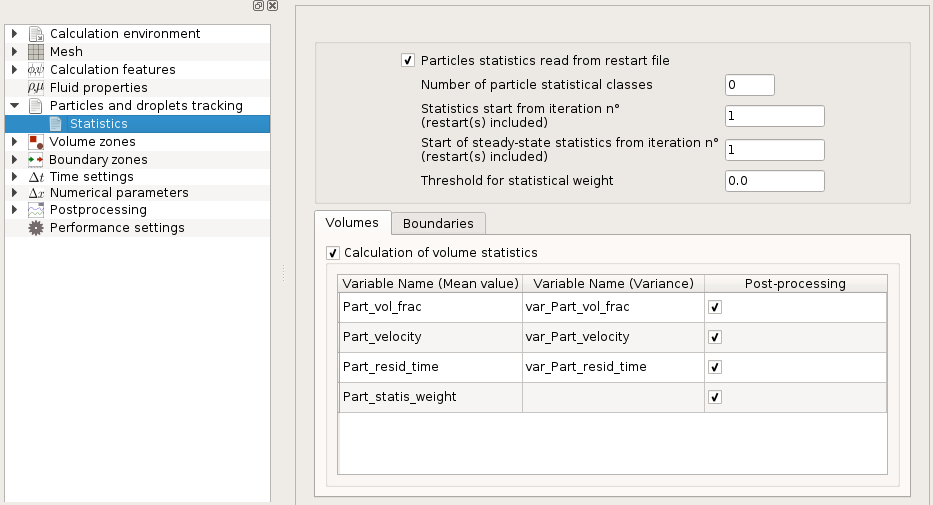
\includegraphics[width=11cm]{gui_lagr_statistics}
% \caption{Lagrangian module - statistics}
% \label{fig:Ini-Lag4}
% \end{center}
% \end{figure}
%
% \begin{figure}[ht]
% \begin{center}
% 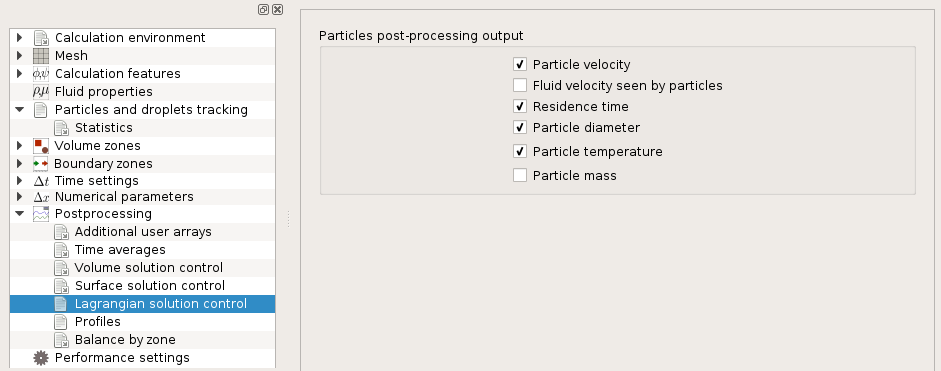
\includegraphics[width=11cm]{gui_lagr_output}
% \caption{Lagrangian module - output}
% \label{fig:Ini-Lag5}
% \end{center}
% \end{figure}

\minititre{Use of the subroutine \texttt{cs\_user\_lagr\_model}}

\noindent
When the GUI is not used, \texttt{cs\_user\_lagr\_model} must be completed. This function
gathers in different headings all the keywords which are
necessary to configure the Lagrangian module. The different headings refer to:
\begin{list}{$\bullet$}{}
\item the global configuration parameters
\item the specific physical models describing the particle behaviour
\item the backward coupling (influence of the dispersed phase on the
      continuous phase)
\item the numerical parameters
\item the volumetric statistics
\item the boundary statistics
\end{list}
%
\noindent
For more details about the different parameters, the user may refer to the
keyword list (\S~\ref{sec:prg_motscles_lagr}).%FIXME


%==================================
\subsubsection{Prescribing particle boundary conditions (GUI and/or \texttt{cs\_user\_lagr\_boundary\_conditions.c})}
%==================================
In the framework of the multiphase Lagrangian modelling, the management of the boundary conditions concerns the particle behaviour when there is an interaction between its trajectory and a boundary face. These boundary conditions may be imposed independently of those concerning the Eulerian fluid phase (but they are of course generally consistent). The boundary condition zones are actually redefined by the Lagrangian module (cf. \S\ref{sec:fvm_selector}), and a type of particle behaviour is associated with each one. The boundary conditions related to particles can be defined in the Graphical User Interface (GUI) or in the \texttt{cs\_user\_lagr\_boundary\_conditions.c} file. More advanced user-defined boundary conditions can be prescribed in the \texttt{cs\_user\_lagr\_in function} from \texttt{cs\_user\_lagr\_particle.c}.

\minititre{Use of the GUI}

 In the GUI, selecting the Lagrangian module in the activates the item \texttt{Particle boundary conditions} under the heading \texttt{Boundary conditions} in the tree menu. Different options are available depending on the type of standard boundary conditions selected (wall, inlet/outlet, etc...),
 see \figurename~\ref{fig:CL-Lag}.

\begin{figure}[ht]
\begin{center}
\includegraphics[width=0.9\textwidth]{gui_lagr_bc}
\caption{Lagrangian module - boundary conditions}
\label{fig:CL-Lag}
\end{center}
\end{figure}

%==================================
\subsubsection{Advanced particle-tracking set-up}
%==================================

In this section, some information is provided for a more advanced numerical set-up of a particle-tracking simulation.

\minititre{User-defined stochastic differential equations}
%-------------------------------------------------

\noindent
An adaptation in the \texttt{cs\_user\_lagr\_sde} function is required if
supplementary user variables are added to the particle state vector.
This function is called at each Lagrangian sub-step.

\noindent
The integration of the stochastic differential equations associated with
supplementary particulate variables is done in this function. \\
When the integration scheme of the stochastic differential equations is
a first-order (\texttt{nordre} = 1), this subroutine is called once every
Lagrangian iteration, if it is a second-order (\texttt{nordre} = 2), it is called
twice. \\

\noindent
The solved stochastic differential equations must be written in the
form:
\begin{displaymath}
\frac{d \Phi_p}{dt} \,=\, - \frac{\Phi_p - \Pi}{\tau_\phi}
\end{displaymath}
where $\Phi_p$ is the I\textit{th} supplementary user variable,
$\tau_\phi$ is a quantity homogeneous to a characteristic time, and $\Pi$ is
a coefficient which may be expressed as a function of the other
particulate variables. \\
In order to do the integration of this equation, the following
parameters must be provided:
\begin{list}{-}{}
\item $\tau_\phi$, equation characteristic time
      every particle,
\item $\Pi$ , equation coefficient. If the
      integration scheme is a first-order, then $\Pi$ is expressed as a
      function of the particulate variables at the previous iteration,
      stored in the array \texttt{eptpa}. If the chosen scheme is a second-order,
      then $\Pi$ is expressed at the first call of the function
      (prediction step) as a function of the variables at the
      previous iteration, then at the second call
      (correction step) as a function of the predicted variables.
\end{list}

\noindent
If necessary, the thermal characteristic time $\tau_c$, whose calculation can be modified by the user in the function
\texttt{cs\_user\_lagr\_rt}.

\minititre{User-defined particle relaxation time}
%-------------------------------------------------

\noindent
The particle relaxation time may be modified in the \texttt{cs\_user\_lagr\_rt} function according to the chosen formulation of the drag coefficient. The particle relaxation time, modified or not by the user, is available in the array \texttt{taup}.

\minititre{User-defined particle thermal characteristic time}
%-------------------------------------------

\noindent
The particle thermal characteristic time may be modified in the \texttt{cs\_user\_lagr\_rt\_t} function according to the chosen correlation for the calculation of the
Nusselt number. This function is called at each Lagrangian sub-step.


%==================================
\subsection{Compressible module}
%==================================

When the compressible module\footnote{For more details concerning the
compressible version, the user may refer to the theory guide \cite{theory} and the document ``Implantation
d'un algorithme compressible dans \CS'', Rapport EDF 2003,
HI-83/03/016/A, P. Mathon, F. Archambeau et J.-M. H\'erard.} is
activated, it is recommended to:
\begin{list}{-}{}
 \item use the option ``time step variable in time and uniform in
       space'' (\texttt{idtvar}=1) with a maximum Courant number of 0.4
       (\texttt{coumax}=0.4): these choices must be written in \texttt{cs\_user\_parameters.f90}
       or specified with the GUI.
 \item keep the convective numerical schemes proposed by default (\textit{i.e.}: upwind scheme).
\end{list}
With the compressible algorithm, the specific total energy is a new solved variable
\texttt{isca(ienerg)}). The temperature variable deduced from the specific
total energy variable is \texttt{isca(itempk)} for the compressible module.\\
Initialisation of the options of the variables, boundary conditions, initialisation of the variables and
management of variable physical properties can be done with the GUI. We describe below the subroutines
the user has to fill in without the GUI.

%==================================
\subsubsection{ Initialisation of the options of the variables}
%==================================
\label{prg_uscfx12}%
\noindent
\textit{Subroutines called at each time step.}

When the GUI is not being used, the subroutines \texttt{uscfx1} and \texttt{uscfx2} in \texttt{cs\_user\_parameters.f90}
must be completed by the user.

\texttt{uscfx1} allows to specify:
\begin{list}{-}{}
\item \texttt{ieos}: equation of state (only perfect gas with a constant adiabatic coefficient,
                      \texttt{ieos=1} is available, but the user can complete the subroutine
                      \texttt{cfther}, which is not a user subroutine, to add new equations of state).
\item \texttt{call field\_set\_key\_int(ivarfl(isca(itempk)), kivisl, ...)}: molecular thermal conductivity, constant (\texttt{-1}) or variable (\texttt{0}).
\item  \texttt{iviscv}: volumetric molecular viscosity, constant (\texttt{0}) or variable (\texttt{1}).
\end{list}

\texttt{uscfx2} allows to specify:
\begin{list}{-}{}
  \item \texttt{ivivar}: molecular viscosity, constant (\texttt{0}) or variable (\texttt{1}).
  \item \texttt{visls0(itempk)}: reference molecular thermal conductivity.
  \item \texttt{viscv0}: reference volumetric molecular viscosity.
  \item \texttt{xmasmr}: molar mass of the perfect gas (\texttt{ieos=1}).
  \item \texttt{icfgrp}: specify if the hydrostatic equilibrium must be accounted for in the
                         boundary conditions.
\end{list}

%==================================
\subsubsection{Management of the boundary conditions}
%==================================

\noindent
\textit{Subroutine called at each time step.}

When running the compressible module without a GUI, the \texttt{cs\_user\_boundary\_conditions} subroutine can be used to define specific boundary conditions
(see the \texttt{cs\_user\_boundary\_conditions-compressible} file in the directory \texttt{EXAMPLES}
for examples of boundary conditions with the compressible module).

With the compressible module, the following types of boundary condition are avaliable:

\begin{list}{-}{}
  \item Inlet/outlet for which velocity and two thermodynamics variables are known.
  \item Subsonic inlet with imposed total pressure and total energy.
  \item Subsonic outlet with imposed static pressure.
  \item Supersonic outlet.
  \item Wall (adiabatic or not).
  \item Symmetry.
\end{list}

It is advised to only use these predefined boundary conditions type for the compressible module.

%==================================
\subsubsection{Initialisation of the variables}
%==================================

\noindent
\textit{Subroutine called only at the initialisation of the calculation}

When the GUI is not used, the subroutine \texttt{cs\_user\_initialization} is used
initialize the velocity, turbulence and passive scalars (see
the \texttt{cs\_user\_initialization-compressible} file in the directory \texttt{EXAMPLES}
for examples of initialisations with the compressible module). Concerning
pressure, density, temperature and specific total energy, only 2 variables out
of these 4 are independent. The user may then initialise the desired variable pair
(apart from temperature-energy) and the two other variables will be
calculated automatically by giving the right value to the variable
\texttt{ithvar} used for the call to the subroutine \texttt{cfther}.

%==================================
\subsubsection{Management of variable physical properties}
%==================================

\noindent
\textit{Subroutine called at each time step.}

Without the GUI, all of the laws governing the physical properties of the fluid
(molecular viscosity, molecular volumetric viscosity, molecular thermal conductivity and
molecular diffusivity of the user-defined scalars) can be specified in the subroutine \texttt{usphyv} of
the \texttt{cs\_user\_physical\_properties} file,
which is then called at each time step. This subroutine replaces and is similar to \texttt{usphyv}.

The user should check that the defined laws are valid for
the whole variation range of the variables. Moreover, as only the perfect gas with a constant
adiabatic coefficient equation of state is available, it is not advised to give a law for the isobaric
specific heat without modifying the equation of state in the subroutine \texttt{cfther} which is not
a user subroutine.

%==================================
\subsection{Management of the electric arcs module}
%==================================

%==================================
\subsubsection{Activating the electric arcs module}\label{sec:acti-lag}
%==================================

The electric arcs module is activated either:
%
\begin{itemize}
 \item [$\bullet$] in the Graphical User Interface (GUI): \texttt{Calculation features} $\rightarrow$ \texttt{Electrical models}
 \item [$\bullet$] or in the user subroutine \texttt{usppmo}, by setting the \texttt{ielarc} or \texttt{ieljou} parameter to a non-null value.
\end{itemize}

%==================================
\subsubsection{Initialisation of the variables}
%==================================

\noindent
\textit{Subroutine called only at initialisation of the calculation}

The subroutine \texttt{cs\_user\_initialization} allows the user to initialise some of the specific physics variables prompted via \texttt{usppmo}. It is called only during the initialisation of the calculation. As usual,the user has access to many geometric variables so
 that the zones can be treated separately if needed.

The values of potential and its constituents are initialised if required.

It should be noted that the enthalpy is relevant.

\begin{list}{-}{}
\item For the electric arcs module, the enthalpy value is taken from the temperature
 of reference \texttt{t0} (given in \texttt{cs\_user\_parameters.f90}) from the temperature-enthalpy
 tables
 supplied in the data file \texttt{dp\_ELE.} The user must not intervene here.
\item For the Joule effect module, the value of enthalpy must be specified by the user
. An example is given of how to obtain the enthalpy from the temperature of reference
 \texttt{t0}(given in \texttt{cs\_user\_parameters.f90}), the temperature-enthalpy law must be
supplied. A code is suggested in the \texttt{usthht} subroutine (provided for
 the determination of physical properties).
\end{list}

%==================================
\subsubsection{Variable physical properties}
%==================================

All the laws of the variation of physical data of the fluid are written (when necessary)
in the subroutine \texttt{cs\_user\_physical\_properties}. It is called at each time step.

{\em WARNING: For the electric module, it is here that all the physical variables are defined
 (including the relative cells and the eventual user scalars):} \texttt{cs\_user\_physical\_properties} {\em {is not used.}}

The user should ensure that the defined variation laws are valid for the whole range of
variables. Particular care should be taken with non-linear laws (for example, a
 $3^{rd}$ degree polynomial law giving negative values of density)

{\em WARNING: In the electric module, all of the physical properties are considered as variables
 and are therefore stored using the \texttt{cs\_field} API. \texttt{cp0}, \texttt{viscls0} and \texttt{viscl0}
 are not used}

For the Joule effect, the user is required to supply the physical properties in the
subroutine. Examples are given which are to be adapted by the user. If the temperature is
to be determined to calculate the physical properties, the solved variable, enthalpy must
 be deduced. The preferred temperature-enthalpy law can be selected in the subroutine
 \texttt{usthht} (an example of the interpolation is given from the law table. This
subroutine can be re-used for the initialisation of the variables(\texttt{cs\_user\_initialization}))
 For the electric arcs module, the physical properties are interpolated from the data file
 \texttt{dp\_ELE} supplied by the user. Modifications are generally not necessary.

%==================================
\subsubsection{Boundary conditions}
%==================================

For the electric module,each boundary face in \texttt{cs\_user\_boundary\_conditions} should be associated with a
 \texttt{izone} number \footnote{\texttt{izone} must be less than the maximum
 value allowed by the code, \texttt{nozzppm}. This is fixed at 2000 in \texttt
{ppvar} and cannot be modified.}(the color \texttt{icoul} for example) in
 order to group together all the boundary faces of the same type. In the
 \texttt{cs\_user\_boundary\_conditions} report, the main change from the users point of view concerns the
 specification of the boundary conditions of the potential, which isn't
 implied by default. The Dirichlet and Neumann conditions must be imposed
 explicitly using \texttt{icodcl} and \texttt{rcodcl} (as would be done for
 the classical scalar).

Furthermore, if one wishes to slow down the power dissipation (Joule
effect module) or the current (electric arcs module) from the imposed values
\texttt{(puismp\index{puismp}} and \texttt{couimp\index{couimp}} respectively),
 they can be changed by the potential scalar as shown below:

\begin{list}{-}{}
\item For the electric arcs, the imposed potential difference can be a fixed variable:
 for example, the cathode can be fixed at 0 and the potential at the anode
 contains the variable \texttt{dpot}. This variable is initialised in
in \texttt{cs\_user\_parameters.c}
 by an estimated potential difference. If \texttt{ielcor}=1 (see
 \texttt{cs\_user\_parameters.c}), \texttt{dpot} is updated automatically during the
 calculation to obtain the required current.
\item For the Joule effect module, \texttt{dpot} is again used with the same
 signification as in the electric arcs module. If \texttt{dpot} is not wanted
 in the setting of the boundary conditions, the variable \texttt{coejou} can be
 used. \texttt{coejou} is the coefficient by which the potential difference is
 multiplied to obtain the desired power dissipation. By default this begins at
 1 and is updated automatically. If \texttt{ielcor}=1 (see \texttt
{cs\_user\_parameters.c}), multiply the imposed potentials in
\texttt{cs\_user\_boundary\_conditions} by \texttt{coejou} at each time step to
achieve the desired power dissipation.
 \end{list}

 {\em WARNING: In the case of alternating current, attention should be paid to the values of potential
 imposed at the limits: the variable named "real potential" represents an affective
 value if the current is in single phase, and a "real part" if not.}
\begin{list}{-}{}
\item For the Joule studies, a complex potential is sometimes needed
 (\texttt{ippmod(ieljou)}=2): this is the  case in particular where the current
 has three phases. To have access to the phase of the potential, and not just to its
 amplitude, the two variables must be deleted: in \CS, there are two arrays
 specified for this role, the real part and the imaginary
 part of the potential. For use in the code, these variables are named
 ``real potential'' and ``imaginary potential''. For an alternative
 sinusoidal potential $Pp$, the maximum value is noted as $Pp_\text{max}$,
 the phase is noted as $\phi$, the real potential
 and the imaginary potential are respectively $Pp_\text{max}\,cos\phi$ and
$Pp_\text{max}\,sin\phi$.
\item For the Joule studies in which one does not have access to the phases, the real
 potential (imaginary part =0) will suffice (\texttt{ippmod(ieljou)=1}): this is
 obviously the case with
 continuous current, but also with single phase alternative current. In \CS
there is only 1 variable for the potential,  called "real potential". Pay attention to
 the fact that in alternate current, the "real potential" represents a effective value
 of potential , $\frac{1}{\sqrt{2}}\,Pp_\text{max}$ (in continuous current there is no
 such ambiguity).
\end{list}

\minititre{Additions for transformers}

The following additional boundary conditions must be defined for tansformers:
\begin{list}{$\bullet$}{}
\item  the intensity at each electrode
\item  the voltage on each terminal of transformers. To achieve it, the intensity,
 the rvoltage at each termin, the Rvoltage, and the total intensity of the
transformer are calculated.
\end{list}

Finally, a test is performed to check if the offset is zero or if a boundary
 face is in contact with the ground.

%====================================
\subsubsection {Initialisation of the variable options}
%==================================
\label{prg_cs_user_parameters}%

The subroutine \texttt{cs\_user\_parameters} (in \texttt{cs\_user\_parameters.c})
 is called at each time step. It allows:
\begin{list}{$\bullet$}{}
\item to give the coefficient of relaxation of the density \texttt{srrom}:\\
$\rho^{n+1}=\texttt{srrom}*\rho^{n}+(1-\texttt{srrom})\rho^{n}$\\
(for the electric arcs, the sub-relaxation is taken into account during the 2nd time
 step;)

\item to indicate if the data will be fixed in the power dissipation or
 in the current, done in \texttt{ielcor}.
\item target either the current fixed as \texttt{couimp} (electric arcs module)
 or the power dissipation \texttt{puism} (Joule module effect).
\item to fix the initial value of potential difference \texttt{dpot},
 the for the calculations with a single fixed parameter as \texttt{couimp}
 or \texttt{puism}.
\item to define type of scaling model for electric arcs \texttt{modrec}. If scaling
by a resetting plane is choosen then \texttt{idreca} defines the current density component
and \texttt{crit\_reca} the plane used for resetting of electromagnetic variables.
\end{list}

%==================================
\subsubsection[{\em EnSight} output]
{Post-processing output}
%==================================

The algebraic variables related to the electric module are provided by default:
\begin{list}{-}{}
\item gradient of real potential in $V m^{-1}$ ($\grad Pot_R = -\vect{E}$)
\item density of real current in $A m^{-2}$  ($\vect{j}=\sigma \vect{E}$)
\end{list}
specifically for the Joule module effect with \texttt{ippmod(ieljou)}=2~:
\begin{list}{-}{}
\item gradient of imaginary potential in $V m^{-1}$
\item density of real current in $A m^{-2}$
\end{list}
specifically for the electric arcs module with \texttt{ippmod(ielarc)}=2~:
\begin{list}{-}{}
\item magnetic field in $T$ (\vect{B} = \vect{rot}\,\vect{A})
\end{list}

The post-processing output will be created automatically (on all output volume
meshes for which the automatic output of main variables is active).

%==================================
\subsection{\CS-\CS coupling}
%==================================

\noindent
\textit{Subroutine called once during the calculation initialisation.}

The user function \texttt{cs\_user\_saturne\_coupling} (in
 \texttt{cs\_user\_coupling.c} is used to couple \CS with itself.
 It is used for turbo-machine applications for instance, the first \CS managing
 the fluid around the rotor and the other the fluid around the stator.
In the case of a coupling between two \CS instances, first argument \texttt{saturne\_name}
 of the function '\texttt{cs\_sat\_coupling\_define}' is ignored.
 In case of multiple couplings, a coupling will be matched with available \CS
 instances based on that argument, which should match the directory name for the
 given coupled domain..\\
The arguments of '\texttt{cs\_sat\_coupling\_define}' are:
\begin{list}{-}{}
\item \texttt{saturne\_name}: the matching \CS application name,
\item \texttt{volume\_sup\_criteria}: the cell selection criteria for support,
\item \texttt{boundary\_sup\_criteria}: the boundary face selection criteria for support (not functional),
\item \texttt{volume\_cpl\_criteria}: the cell selection criteria for coupled cells,
\item \texttt{boundary\_cpl\_criteria}: the boundary face selection criteria for coupled faces,
\item \texttt{verbosity}: the verbosity level.
\end{list}


%==================================
\subsection{Fluid-Structure external coupling}
%==================================

\noindent
\textit{Subroutine called only once}

The subroutine \texttt{usaste} belongs to the module dedicated to external
 Fluid-Structure coupling with \textit{Code\_Aster}. Here one defines the boundary
 faces coupled with \textit{Code\_Aster} and the fluid forces components which are
 given to structural calculation. When using external coupling with \textit{Code\_Aster},
 structure numbers necessarily need to be negative; the references of coupled faces being
 i.e. -1, -2, \emph{etc.}
The subroutine performs the following operations:
\begin{list}{-}{}
 \item '\texttt{getfbr}' is called to get a list of elements matching a
geometrical criterion or reference number then a structure number (negative value) is associated
 to these elements.
 \item the value passed to \texttt{asddlf}, for user-chosen component, for every negative
 structure number, defines the movement imposed to the external structure.
\end{list}
%
\clearpage
%
%==================================
\subsection{ALE module}
%==================================
%==================================
\subsubsection{Initialisation of the options}
%==================================
This initialisation can be performed in the Graphical User Interface (GUI)
 or in the subroutines \texttt{usipph} and \texttt{usstr1}. Firstly,
 when the ``Mobile mesh'' is selected in GUI under the ``Calculation features''
 heading, additional options are displayed. The user must choose the type of mesh
 viscosity and describe its spatial distribution, see \figurename~\ref{fig:Ini-ale}.
%
\begin{figure}[!ht]
\begin{center}
\includegraphics[width=12cm]{gui_ale_mei}
\caption{Thermophysical models - mobile mesh (ALE method)}
\label{fig:Ini-ale}
\end{center}
\end{figure}
%
The following paragraphs are relevant if the GUI is not used.

\minititre{Subroutine \texttt{usipph}}
\noindent
\textit{Subroutine called at the beginning.}
This subroutine completes \texttt{cs\_user\_parameters.f90}.

\texttt{usipph} allows setting options for the ALE module, and in
particular to activate the ALE module (\texttt{iale=1}).

\minititre{Subroutine \texttt{usstr1}}

This subroutine reads in \texttt{cs\_user\_fluid\_structure\_interaction.f90}. It allows to specify the following pieces of information for the structure module:
\begin{list}{-}{}
  \item the index of the structure, (\texttt{idfstr(ifac)} where \texttt{ifac} is the index of the face). Then the total number of structures \texttt{nbstru} is automatically computed by the code. Be careful, the value must belong to 1, ..., \texttt{nbstru}.
  \item the initial value of displacement, velocity and acceleration
    (\texttt{xstr0}, \texttt{xstreq} and \texttt{vstr0}).
\end{list}

Below is a list of the different variables that might be modified:

\begin{list}{$\bullet$}{}

\item{\texttt{idfstr(ifac)}} \\
{the index of the structure, (\texttt{idfstr(ifac)} where \texttt{ifac} is the index of the face), 0 if the face is not coupled to any structure.}

\item{\texttt{xstr0(i,k)}} \\
{initial position of a structure, where \texttt{i} is the dimension of space
and \texttt{k} the index of the structure}

\item{\texttt{xstreq(i,k)}} \\
{equilibrum position of a structure, where \texttt{i} is the dimension of space
and \texttt{k} the index of the structure}

\item{\texttt{vstr0(i,k)}} \\
{initial velicity of a structure, where \texttt{i} is the dimension of space
and \texttt{k} the index of the structure }
\end{list}

%==================================
\subsubsection{Mesh velocity boundary conditions}
%==================================
These boundary conditions can be managed through the Graphical User Interface (GUI)
 or using the subroutine \texttt{usalcl} (called at each time step). With the GUI,
 when the item ``Mobile mesh'' is activated  the item ``Fluid structure interaction''
 appears under the heading ``Boundary conditions''. Two types of fluid-structure
 coupling are offered. The first one is internal, using a simplified structure
 model and the second is external with \textit{Code\_Aster}, see \figurename~
 \ref{fig:CL-ale1} and \figurename~\ref{fig:CL-ale2}.
%
\begin{figure}[ht]
\begin{center}
\includegraphics[width=0.9\textwidth]{gui_ale_internal}
\caption{Boundary conditions - internal coupling}
\label{fig:CL-ale1}
\end{center}
\end{figure}
%
\begin{figure}[ht]
\begin{center}
\includegraphics[width=0.9\textwidth]{gui_ale_external}
\caption{Boundary conditions - external coupling}
\label{fig:CL-ale2}
\end{center}
\end{figure}

\minititre{Subroutine \texttt{usalcl}}
When the GUI is not used, the use of \texttt{usalcl} is mandatory to run
a calculation using
the ale module just as it is in \texttt{cs\_user\_parameters.f90}. It is used the same way as
\texttt{cs\_user\_boundary\_conditions} in the framework of
standard calculations, that is to say a loop on the boundary faces
marked out by their colour (or more generally by a property of their
family), where the type of mesh velocity boundary condition is definied for
each variable.

The main numerical variables are described below.

\variab{ialtyb}{ialtyb(nfabor)}{ia}{In the ale module, the user
defines the mesh velocity from the colour of the boundary faces, or
more generally from their properties (colours, groups, ...), from the
boundary conditions defined in \texttt{cs\_user\_boundary\_conditions}, or even from their
coordinates. To do so, the array \texttt{ialtyb(nfabor)} gives for each face
\texttt{ifac} the mesh velocity boundary condition types marked out by the key
words \texttt{ivimpo\index{ivimpo}}, \texttt{igliss\index{igliss}},
\texttt{ibfixe\index{ibfixe}} or \texttt{ifresf\index{ifresf}}}.

\begin{list}{$\bullet$}{}

\item If \texttt{ialtyb(ifac) = ivimpo}: imposed velocity.

\begin{list}{$\rightarrow$}{}
\item In the cases where all the nodes of a face have a imposed displacement,
 it is not necessary to fill the tables with mesh velocity boundary conditions
 for this face, these will be erased. In the other case,
 the value of the Dirichlet must be given in \texttt{rcodcl(ifac,ivar,1)} for
 every value of \texttt{ivar} (\texttt{iuma}, \texttt{ivma} and \texttt{iwma}).
 The other boxes of \texttt{rcodcl} and \texttt{icodcl} are completed automatically.

 The tangential mesh velocity is taken like a tape speed under the
 boundary conditions of wall for the fluid, except if wall fluid velocity
 was specified by the user in the interface or \texttt{cs\_user\_boundary\_conditions} (in which case
 it is this speed which is considered).
\end{list}

 \item if \texttt{ialtyb(ifac) = ibfixe}: fixed wall
\begin{list}{$\rightarrow$}{}
 \item the velocity is null.
\end{list}

 \item if \texttt{ialtyb(ifac) = igliss}: sliding wall
\begin{list}{$\rightarrow$}{}
\item symmetry boundary condition on the mesh velocity vector, which means a homogeneous Neumann on the tangential mesh velocity and a zero Dirichlet on the normal mesh velocity.
\end{list}

 \item if \texttt{ialtyb(ifac) = ifresf}: free-surface
\begin{list}{$\rightarrow$}{}
\item an imposed mesh velocity such that the fluid mass flux is equal to the mesh displacement in order to mimic the free-surface automatically. Note that the boundary condition on the fluid velocity must be set separately (homogeneous Neumann conditionfor instance).
\end{list}

\end{list}
}

%==================================
\subsubsection{Modification of the mesh viscosity}
%==================================

The user subroutine \texttt{cs\_user\_physical\_properties} can be used along the ALE (Arbitrary Lagrangian Eulerian
 Method) module, and allows modifying the mesh viscosity.
 It is called before the time loop, and before reading restart files
 (so the mesh is always in its initial position at this stage).
The user can modify mesh viscosity values to prevent cells and nodes from huge
 displacements in awkward areas, such as boundary layer for example.

Note that for more complex settings, the mesh viscosity could be modified in
 \texttt{cs\_user\_initialization} or \texttt{cs\_user\_extra\_operations}.
 The matching field's name is \texttt{mesh\_viscosity}.

%==================================
\subsubsection{Fluid - Structure internal coupling}\label{sec:ALE}
%==================================

In the subroutine \texttt{cs\_user\_fluid\_structure\_interaction} the user provides the parameters of two other subroutines.
\texttt{usstr1} is called at the beginning of the calculation. It is used to define
 and initialise the internal structures where fluid-Structure coupling occurs.
For each boundary face \texttt{ifac}, \texttt{idfstr(ifac)} is the index of the structure
 the face belongs to (if \texttt{idfstr(ifac)} = 0, the face \texttt{ifac} doesn't belong
 to any structure). When using internal coupling, structure index necessarily must be
 strictly positive and smaller than the number of structures. The number of "internal" structures is automatically defined with the maximum
 value of the \texttt{idfstr} table, meaning that internal structure numbers must be defined
 sequentially with positive values, beginning with integer value '1'.

For each internal structure the user can define:
\begin{list}{-}{}
 \item an initial velocity \texttt{vstr0}
 \item an initial displacement \texttt{xstr0} ({\em i.e.} \texttt{xstr0} is the value of the
 displacement \texttt{xstr} compared to the initial mesh at time t = 0)
 \item a displacement compared to equilibrium  \texttt{xstreq} (i.e. \texttt{xstreq}
 is the initial displacement of the internal structure compared to its position at
 equilibrium; at each time step t and for a displacement \text{xstr}(t), the associated
 internal structure will undergo a force $-k*(\text{}t+XSTREQ)$ due to the spring).
\end{list}
\text{xstr0} and \text{vstr0} are initialised with the value 0.
When starting a calculation using ALE, or re-starting a calculation with ALE, based
 on a first calculation without ALE, an initial iteration 0 is automatically performed
 in order to take initial arrays \text{xstr0}, \text{vstr0} and \text{xstreq} into
 account. In any other case, add the following expression '\text{italin=1}' in subroutine
 \text{usipsu}, so that the code can deal with the arrays \text{xstr0}, \text{vstr0} and \text{xstreq}.

When \texttt{ihistr} is set to 1, the code writes in the output the history of the
 displacement, of the structural velocity, of the structural acceleration and of the
 fluid force. The value of structural history output step is the same as the one for
 standard variables \text{nthist}.

The second subroutine, \text{usstr2}, is called at each iteration. One defines in this
 subroutine structural parameters (considered as potentially time dependent): {\em i.e.},
 mass m \text{xmstru}, friction coefficients c \text{xcstru}, and stiffness k \text{xkstru}.
 \text{forstr} array gives fluid stresses acting on each internal structure. Moreover it is also
 possible to take external forces (gravity for example ) into account.
\begin{list}{.}{}
 \item the \text{xstr} array indicates the displacement of the structure compared to its position in the initial mesh,
 \item the \text{xstr0} array gives the displacement of the structures in the initial mesh
 compared to structural equilibrium,
 \item the \text{vstr} array stands for structural velocity.
\end{list}
\text{xstr}, \text{xstr0} and \text{vstr} are \text{DATA} tables that can be used to
 define the  Mass, Friction and Stiffness arays. These are not to be modified.

The 3D structural equation that is solved is the following one:
\begin{equation}\label{eq:FluidStruct}
\displaystyle
\tens{m}.\partial_{tt}\vect{x}+\tens{c}.\partial_{t}\vect{x}+\tens{k}.\left(\vect{x}+\vect{x_0}\right)=\vect{f},
\end{equation}
where $x$ stands for the structural displacement compared to initial mesh position
 \text{xstr}, $x_0$ represents
 the displacement of the structure in initial mesh compared to equilibrium.
Note that $\tens{m}$,$\tens{c}$, and $\tens{k}$ are 3\text{x}3 matrices.
Equation \eqref{eq:FluidStruct} is solved using a Newmark HHT algorithm.
Note that the time step used to solve this equation, \text{dtstr}, can be
 different from the one of fluid calculations. The user is free to define \text{dtstr}
 array. At the beginning of the calculation \text{dtstr} is initialised to the value of
 \text{dtcel} (fluid time step).

%==================================
\subsection{Management of the structure property}
%==================================

The use of \texttt{usstr2} is mandatory to run a calculation using the ALE
 module with a structure module. It is called at each time step.

For each structure, the system that will be solved is:

\begin{equation}
M.x^{''}+C.x^{''}+K.(x-x_{0} = 0
\end{equation}

where

\begin{list}{-}{}
 \item $M$ is the mass structure (\texttt{xmstru}).
 \item $C$ is the damping coefficient of the structure (\texttt{xcstru}).
 \item $K$ is the spring constant or force constant of the structure (\texttt{xkstru}).
 \item $x_{0}$ is the initial position.
\end{list}

Below is a list of the different variables that might be modified:

\begin{list}{$\bullet$}{}

\item{\texttt{xmstru(i,j,k})} \\
{mass matrix of the structure, where \texttt{i},\texttt{j} is
the array of mass structure and \texttt{k} the index of the structure.}

\item{\texttt{xcstru(i,j,k})}\\
{damping matrix coefficient of the structure, where \texttt{i},\texttt{j} is the array of
damping coefficient and \texttt{k} the index of the structure.}

\item{\texttt{xkstru(i,j,k)}}\\
{spring matrix constant of the structure, where \texttt{i},\texttt{j} is the array of spring
constant and \texttt{k} the index of the structure.}

\item{\texttt{forstr(i,k)}}\\
{force vector of the structure, where \texttt{i} is the force vector and
\texttt{k} the index of the structure.}
\end{list}

%===========================================================
\subsection{Management of the atmospheric module}
%===========================================================

This section describes how to set a calculation using the atmospheric module
of \CS. Each paragraph describes a step of the data setting process.

\subsubsection{Directory structure}\label{sec:atmo_struct}
%
The flowchart (\figurename~\ref{fig:organisation}) recalls the directory
structure of a study generated by \CS (see also \ref{sec:prg_architecture}).
When using the atmospheric module, the structure is identical but a file called
\texttt{meteo} may be added to the data settings in order to provide vertical
profiles of the main variables. This file should be put in the \texttt{DATA}
directory. For more details about the \texttt{meteo} file, see \S~
~\ref{sec:atmo_BCs}).
%
\begin{figure}[ht]
 \centerline{\includegraphics[width=0.6\textwidth]{gui_atmospheric_user_s_guide_v91.png}}
 \caption{Organization of a study (specific files of atmospheric version in bold type)}
 \label{fig:organisation}
\end{figure}
%
\subsubsection{The atmospheric mesh features}
%
An atmospheric mesh has the following specific features:
%
\begin{itemize}
\item The boundary located at the top of the domain should be a plane.
So, horizontal wind speed at a given altitude can be prescribed at the top
face as an inlet boundary.
\item Cells may have very different sizes, from very small (near ground or
buildings) to very large (near the top of domain or far from zone of interest).
\item Vertical resolution: from tiny cells (e.g. $\Delta $\upshape z = 1 m) near
the ground to a few hundreds of meters at the top.
\item Horizontal resolution: from a few meters to hundreds of meters.
\item The length ratio between two adjacent cells (in each direction) should
preferably be between $0.7$ and $1.3$.
\item The z axis represents the vertical axis.
\end{itemize}
%
A topography map can be used to generate a mesh. In this case, the preprocessor
 mode is particularly useful to check the quality of the mesh (run type Mesh
quality criteria).
%
\subsubsection{Atmospheric flow model and steady/unsteady algorithm}
%
The Graphical User Interface (GUI) may be used to enable the atmospheric flow
module and set up the following calculation parameters in the
\texttt{Thermophysical models}-\texttt{Calculation features} page
(see \figurename~\ref{fig:steady}):
%
\subsubsubsection{The atmospheric flow model}
%
The user can choose one of the following atmospheric flow models:
%
\begin{itemize}
\item \textbf{Constant density}: To simulate neutral atmosphere.
\item \textbf{Dry atmosphere}: To simulate dry, thermally-stratified
atmospheric flows (enables \texttt{Potential temperature} as thermal model).
\item \textbf{Humid atmosphere}: To simulate thermally stratified atmospheric
flows (air-water mixture) with phase changes (enables \texttt{Liquid potential
temperature} as thermal model). The model is described in
Bouzereau \cite{bouzereau}.
\end{itemize}
%
\subsubsubsection{The time algorithm}
%
\begin{itemize}
\item Steady flow algorithm: is the one usually set. It sets a time step
variable in space and time. It has to be selected if constant boundary
conditions are used.
\item Unsteady flow algorithm has to be selected for time varying boundary
conditions (the time step can then be variable in time or constant).
\end{itemize}
%
\begin{figure}[ht]
\centerline{\includegraphics[width=0.7\textwidth]{gui_atmospheric_user_s_guide_v92.png}}
\caption{Selection of atmospheric model}
\label{fig:steady}
\end{figure}
%
\begin{figure}[ht]
\centerline{\includegraphics[width=0.9\textwidth]{gui_atmospheric_user_s_guide_v93.png}}
\caption{Selection of steady/unsteady flow algorithm}
\label{fig:global}
\end{figure}
%
Table \tablename~\ref{tab:param_list} can help to choose the right parameters
depending on the type of atmospheric flow.
%
\subsubsubsection{Warnings}
The following points have to be considered when setting the parameters
described above:
\begin{itemize}
\item The potential temperature thermal model and the liquid potential
temperature one (see the paragraph ``Atmospheric main variables'' for the
definition) requires that the vertical component of the gravity is set to
$g_z=-9.81 m.s^{-2}$ ($g_x=g_y=0 m.s^{-2}$),
otherwise pressure and density won't be correctly computed.
\item As well, the use of scalar with drift for atmospheric dispersion requires
the gravity to be set to $g_z=-9.81$ ($g_x=g_y=0 m.s^{-2}$), even if the density
is constant.
\end{itemize}
%
\subsubsection{Physical properties}
%
The specific heat value has to be set to the atmospheric value
$C_{p}=1005 J/kg/K$.
%
\begin{table}[ht]\label{tab:param_list}
\begin{center}
\begin{tabular}{|p{80pt}|p{70pt}|p{70pt}|p{80pt}|p{100pt}|}
\hline
\textbf{Parameters} & \textbf{Constant density} & \textbf{Dry atmosphere} & \textbf{Humid atmosphere} & \textbf{Explanation} \\
\hline
pressure boundary condition & Neumann first order & Extrapolation & Extrapolation &
In case of \textbf{Extrapolation}, the pressure gradient is assumed (and set) constant, whereas in case of \textbf{Neumann first order},
the pressure gradient is assumed (and set) to zero. \\
\hline
Improved pressure interpolation in stratified flows & no & yes & yes & If yes, exact balance between the hydrostatic part of the pressure gradient and the gravity term $\rho g$ is numerically ensured. \\
\hline
Gravity (gravity is assumed aligned with the z-axis) & $g_z=0$ or $g_z=-9.81 m.s^{-2}$ (the latter is useful for scalar with drift) & $g_z=-9.81 m.s^{-2}$ & $g_z=-9.81 m.s^{-2}$ &  \\
\hline
Thermal variable & no & potential temperature & liquid potential temperature &  \\
\hline
Others variables & no & no & total water content, droplets number &  \\
\hline
\end{tabular}\label{tab1}
\caption[List of parameters]{List of parameters}
\end{center}
\end{table}
%
\subsubsection{Boundary and initial conditions}\label{sec:atmo_BCs}
%
The \texttt{meteo} file can be used to define initial conditions for the
different fields and to set up the inlet boundary conditions. For the velocity
field, \CS can automatically detect if the boundary is an inlet boundary or an
outflow boundary, according to the wind speed components given in the
\texttt{meteo} file with respect to the boundary face orientation. This is often
used for the lateral boundaries of the atmospheric domain, especially if the
profile is evolving in time. In the case of inlet flow, the data given in the
\texttt{meteo} file will be used as the input data (Dirichlet boundary condition)
for velocity, temperature, humidity and turbulent variables. In the case of
outflow, a Neumann boundary condition is automatically imposed (except for the
pressure). The unit of temperature in the \texttt{meteo} file is the degree
Celsius whereas the unit in the GUI is the kelvin.

To be taken into account, the \texttt{meteo} file has to be selected in the GUI
(\texttt{Atmospheric flows} page, see \figurename~\ref{fig:meteo}) and the check
box on the side ticked. This file gives the profiles of prognostic atmospheric
variables containing one or a list of time stamps. The file has to be put in the
\texttt{DATA} directory.
%
\begin{figure}[htbp]
\centerline{\includegraphics[width=0.9\textwidth]{gui_atmo_read.png}}
\caption{Selection of the \texttt{meteo} file}
\label{fig:meteo}
\end{figure}
%
An example of file \texttt{meteo} is given in the directory
\texttt{DATA/REFERENCE/}. The file format has to be strictly respected.
The horizontal coordinates are not used at the present time (except when
boundary conditions are based on several meteorological vertical profiles)
and the vertical profiles are defined with the altitude above sea level. The
highest altitude of the profile should be above the top of the simulation domain
and the lowest altitude of the profile should be below or equal to the lowest
level of the simulation domain. The line at the end of the \texttt{meteo} file
should not be empty.

If the boundary conditions are variable in time, the vertical profiles for
the different time stamps have to be written sequentially in the \texttt{meteo}
file.

You can also set the profiles of atmospheric variables directly in the GUI.
The following boundary conditions can be selected in the GUI:
%
\begin{itemize}
\item Inlet/Outlet is automatically calculated for lateral boundaries
(e.g. North, West\textellipsis ) of the computational domain
(see \figurename~\ref{fig:inlet}).
\item Inlet for the top of the domain (see \figurename~\ref{fig:top}).
\item Rough wall for building walls (see \figurename~\ref{fig:walls}) or for
the ground (see \figurename~\ref{fig:ground}).
The user has to enter the roughness length. In case of variable roughness
length, the user has to provide the land use data and the association
between the roughness length values and land use categories.
\end{itemize}
%
\begin{figure}[htbp]
\centerline{\includegraphics[width=0.9\textwidth]{gui_atmospheric_user_s_guide_v95.png}}
\caption{Selection of automatic inlet/ outlet for boundary conditions }
\label{fig:inlet}
\end{figure}
%
\begin{figure}[htbp]
\centerline{\includegraphics[width=0.9\textwidth]{gui_atmospheric_user_s_guide_v96.png}}
\caption{Selection of the boundary condition for the top of the domain }
\label{fig:top}
\end{figure}
%
\begin{figure}[htbp]
\centerline{\includegraphics[width=0.9\textwidth]{gui_atmospheric_user_s_guide_v97.png}}
\caption{Selection of the boundary condition for building walls}
\label{fig:walls}
\end{figure}
%
\begin{figure}[htbp]
\centerline{\includegraphics[width=0.9\textwidth]{gui_atmospheric_user_s_guide_v98.png}}
\caption{Selection of the boundary condition for the ground}
\label{fig:ground}
\end{figure}

\paragraph{Remark:} If a meteorological file is given, it is used by default to
initialize the variables. If a meteorological file is not given, the user can
use the standard \CS initial and boundary conditions set up but has to be aware
that even small inconsistencies can create very large buoyancy forces and
spurious circulations.

\subsubsubsection{Boundary conditions based on several meteorological vertical profiles}

In some cases, especially when outputs of a mesoscale model are used, you
need to build input boundary conditions from several meteorological vertical
wind profiles. Cressman interpolation is then used to create the boundary
conditions. The following files need to be put in the \texttt{DATA} directory:
\begin{itemize}
\item All \texttt{meteo} files giving the different vertical profiles of
prognostic variables (wind, temperature, turbulent kinetic energy and
dissipation).
\item A file called \texttt{imbrication\_files\_list.txt} which is a list
of the \texttt{meteo} files used.
\item A separate \texttt{meteo} file which is used for the initial conditions
and to impose inlet boundary conditions for the variables for which Cressman
interpolation is not used (for example: temperature, turbulent kinetic energy).
This file must follow the rules indicated previously.
\end{itemize}
The following files should be put in the SRC directory:
\begin{itemize}
\item The user source file \texttt{cs\_user\_parameters.f90}. In this file, set
the \texttt{cressman\_} flag of each variable, for which the Cressman
interpolation should be enabled, to \texttt{.true.}.
\end{itemize}
%
\subsubsection{User subroutines}
%
The user subroutines are used when the graphical user interface is not
sufficient to set up the calculation. We give some examples of user file for
atmospheric application:
\begin{itemize}
\item \texttt{cs\_user\_source\_terms.f90}: to add a source term in the
prognostic equations for forest canopy modelling, wind turbine wake modelling...
See the associated \doxygenfile{cs_user_source_terms.html}{\texttt{doxygen} documentation
for examples of use of \texttt{cs\_user\_source\_terms.f90}}.
\item \texttt{cs\_user\_parameters.f90}: to activate the Cressman interpolation.
For example, it is used to impose inhomogeneous boundary conditions. See the associated
\doxygenfile{f_parameters.html}{\texttt{doxygen} documentation for examples of use of
\texttt{cs\_user\_parameters.f90}}.
\item \texttt{cs\_user\_extra\_operations-extract.f90}: to generate vertical
profiles for post processing. See the associated
\doxygenfile{cs_user_extra_operations_examples.html}{\texttt{doxygen} documentation
for examples of use of \texttt{cs\_user\_extra\_operations.f90}}.
\item \texttt{cs\_user\_boundary\_conditions-atmospheric.f90}: show how to set
up the boundary conditions and to put a heterogeneous roughness length...
See the associated \doxygenfile{cs_user_boundary_conditions_examples.html}{\texttt{doxygen}
documentation for examples of use of \texttt{cs\_user\_boundary\_conditions.f90}}.
\end{itemize}
%
\paragraph{Remark:}
If the computation is set without the GUI, other user subroutines such as the
following have to be used:
\begin{itemize}
\item \texttt{cs\_user\_initialization-atmospheric.f90}: allows to initialize
or modify (in case of a restarted calculation) the calculation variables and
the values of the time step. See the associated
\doxygenfile{user_initialization.html}{\texttt{doxygen} documentation for
examples of use of \texttt{cs\_user\_initialization.f90}}.

\item \texttt{cs\_user\_boundary\_conditions-atmospheric.f90}: allows to define
all the boundary conditions. For each type of boundary condition, faces should
be grouped as physical zones characterized by an arbitrary number \texttt{izone}
chosen by the user. If a boundary condition is retrieved from a meteorological
profile, the variable \texttt{iprofm(izone)} of the zone has to be set to 1.
The vertical profiles of atmospheric variables can be described in this file.
\end{itemize}
%
Examples are available in the directory \texttt{SRC/EXAMPLE}.
%
\subsubsection{Physical models}
%
\subsubsubsection{Atmospheric dispersion of pollutants}
%
To simulate the atmospheric dispersion of pollutant, one first need to define
the source(s) term(s). That is to say the location i.e. the list of cells or
boundary faces, the total air flow, the emitted mass fraction of pollutant,
the emission temperature and the speed with the associated turbulent parameters.
The mass fraction of pollutant is simulated through a user added scalar that
could be a `scalar with drift' if wanted (aerosols for example).

The simulations can be done using 3 different methods:
\begin{enumerate}
\item Using a mass source term, that is added in the Navier-Stokes
equations using the \texttt{cs\_user\_mass\_source\_terms.f90} user subroutine.

\item Prescribing a boundary condition code ``total imposed mass flux`` for
some boundary faces using the \texttt{cs\_user\_boundary\_conditions.f90} user
subroutine.

\item Using a scalar source term. In this case, the air inflow is not taken
into account. The user has to add an explicit part to the equations
for the scalar through the \texttt{cs\_user\_source\_terms.f90} file. This is
done by selecting the cells and adding the source term \texttt{crvexp (cells)}
which equals to the air flux multiplied by the mass fraction, while the
implicit part \texttt{crvimp} is set to zero.
\end{enumerate}

The first method is recommended, but one must take care that each source
influences the dispersion of the others, which is physically realistic. So
if the impact of several sources has to be analyzed independently it has first
to be verified that these influences are negligible or as many simulations
as there are sources have to be run.

With the second method, the same problem of sources interactions appears, and
moreover standard Dirichlet conditions should not be used (use
\texttt{itypfb=i\_convective\_inlet} and \texttt{icodcl=13} instead) as
the exact emission rate cannot be prescribed because the diffusive part
(usually negligible) cannot be quantified. Additionally, it requires that
the boundary faces of the emission are explicitly represented in the mesh.

Finally the third method does not take into account the jet effect of the
emission and so must be used only if it is sure that the emission does not
modify the flow.

Whatever solution is chosen, the mass conservation should be verified by using
for example the
\texttt{cs\_user\_extra\_operations-scalar\_balance\_by\_zone.f90} file.

\subsubsubsection{Soil/atmosphere interaction model}

This model is based on the force restore model (Deardorff \cite{deardorff}).
It takes into account heat and humidity exchanges between the ground and the
atmosphere at daily scale and the time evolution of ground surface temperature
and humidity. Surface temperature is calculated with a prognostic equation
whereas a 2-layers model is used to compute surface humidity.

The parameter \texttt{iatsoil} in the file \texttt{atini0.f90} needs to be equal to one to
activate the model. Then, the source file \texttt{solvar.f90} is used.

Three variables need to be initialized in the file \texttt{atini0.f90}: deep soil
temperature, surface temperature and humidity.

The user needs to give the values of the model constants in the file
\texttt{solcat.f90}: roughness length, albedo, emissivity...

In case of a 3D simulation domain, land use data has to be provided for the domain.
Values of model constants for the land use categories have also to be
provided.

\subsubsubsection{Radiative model (1D)}

The 1D-radiative model calculates the radiative exchange between different
atmospheric layers and the surface radiative fluxes.

The radiative exchange is computed separately for two wave lengths intervals

\begin{itemize}
\item Calculation in the infrared spectral domain (file \texttt{rayir.f90})
\item Calculation in the spectral range of solar radiation (file
\texttt{rayso.f90})
\end{itemize}
This 1D-radiative model is needed if the soil/atmosphere interaction model
is activated.

This model is activated if the parameter \texttt{iatra1} is equal to one in the
file \texttt{cs\_users\_parameters.f90}.

\subsubsection{Atmospheric main variables}

For more details on the topic of atmospheric boundary layers, see  Stull
\cite{stull}.
%
\begin{itemize}
\item Definition of the potential temperature:
\[
\theta =T\left(\frac{P}{P_{r}}\right)^{-\frac{R_{d}}{C_{p}}}
\]
\item Definition of liquid potential temperature:
\[
\theta_{l} = \theta \left( 1-\frac{L}{C_{p}T} q_{l} \right)
\]
\item Definition of virtual temperature:
\[
T_{v} = \left(1+0.61q\right)T
\]
\item Gas law:
\[
P = \rho \frac{R}{M_{d}}\left(1+0,61q\right)T
\]
with $R=R_{d} M_{d}$.
\item Hydrostatic state:
\[
\frac{\partial P}{\partial z} = -\rho g
\]
\end{itemize}
%
\begin{table}[htbp]
\begin{center}
\begin{tabular}{|l|l|l|l|}
\hline
\textbf{Constant name} & \textbf{Symbol} & \textbf{Values} & \textbf{Unit} \\
\hline
Gravity acceleration at sea level & $g$ & $9.81$ & $m.s^{-2}$ \\
\hline
Effective Molecular Mass for dry air & $M_{d}$ & $28.97$ & $kg.kmol^{-1}$ \\
\hline
Standard reference pressure & $P_{r}$ & $10^{5}$ & $Pa$ \\
\hline
Universal gas constant & $R$ & $8.3143$ & $J.K^{-1}.mol$ \\
\hline
Gas constant for dry air & $R_{d}$ & $287$ & $J.kg^{-1}.K^{-1}$ \\
\hline
\end{tabular}\label{tab2}
\end{center}
\caption{Constant name}
\end{table}

\begin{table}[htbp]
\begin{center}
\begin{tabular}{|l|p{113pt}|}
\hline
\textbf{Variable name} &\textbf{Symbol} \\
\hline
Specific heat capacity of dry air & $C_{p}$ \\
\hline
Atmospheric pressure & $P$ \\
\hline
Specific humidity & $q$ \\
\hline
Specific content for liquid water & $q_{l}$ \\
\hline
Temperature & $T$ \\
\hline
Virtual temperature & $T_{v}$ \\
\hline
Potential temperature & $\theta$ \\
\hline
Liquid potential temperature & $\theta_{l}$ \\
\hline
Latent heat of vaporization & $L$ \\
\hline
Density & $\rho $ \\
\hline
Altitude & $z$ \\
\hline
\end{tabular}\label{tab3}
\caption{Variable name}
\end{center}
\end{table}
%
\subsubsection{Recommendations}\label{subsubsec:recommendations}
%
This part is a list of recommendations for atmospheric numerical simulations.
%
\begin{itemize}
\item Enough probes at different vertical levels in the domain should be used
to check the convergence of the calculation.
\item An inflow boundary condition at the top level of the domain should be set
(symmetry and automatic inlet/outlet are not appropriate).
\item A Courant number too small or too big has to be avoided (see \CS Best
Practice Guidelines). That is the reason why the option \texttt{variable time
step in space and in time} is recommended for steady simulations when there are
large differences of cell size inside the domain (which is generally the case
for atmospheric simulations). With this option, it can be necessary to change
the reference time step and the time step maximal increase (by default, the time
step increase rate is $10\%$).
\end{itemize}
%
In some cases, results can be improved with the following modifications:
%
\begin{itemize}
\item In some case, the turbulent eddy viscosity can drop to unrealistically low
values (especially with $k-\varepsilon$ model in stable atmospheric condition).
In those cases, it is suggested to put an artificial molecular viscosity around
$0.1 m^{2}.s^{-1}$.
\item If the main direction of wind is parallel to the boundary of your computing
domain, try to set symmetry boundary conditions for the lateral boundaries to
avoid inflow and outflow on the same boundary zone (side of your domain).
Another possibility is to use a cylindrical mesh.
\item To avoid inflow and outflow on the same boundary zone (side of your domain),
avoid the case of vertical profile in the input data \texttt{meteo} file with
changes of the sign of velocity of wind ($V_x$ or/and $V_y$).
\end{itemize}

%==================================
%\subsection{Cooling tower modelling}
%==================================

%==================================
%\subsubsection{Parameters}
%==================================

%\noindent
%\textit{Subroutine called only during calculation initialisation? OR AT EACH ITERATION?.}

%The subroutine \texttt{uscti1} contains calculation parameters such as:
%\begin{list}{-}{}
% \item  temperature parameters,
% \item  the number of exchange zones at various locations,
% \item  the air properties.
%\end{list}

%==================================
%\subsubsection{Initialisation of the variables}
%==================================

%With the additional variables introduced with the air-cooling module, the
%following quantities may be initialized by  \texttt{cs\_user\_initialization} in
%user selected zones in addition to the usual quantities:
%\begin{list}{-}{}
% \item the air temperature, variable of index \texttt{isca(ihumid)},
% \item the air humidity, variable of index \texttt{isca(itemp4)},
%\end{list}
%where \texttt{iel} can be an element found in a list returned by the routine
% '\texttt{getcel}'.

%==================================
%\subsubsection{Definition of the exchange zones}
%==================================

%The subroutine \texttt{usctdz} is used to define the exchange zones of a cooling
% tower. The user provides the following parameters:
%\begin{list}{-}{}
% \item \texttt{imzech}: its value is related to the model used:
%      \begin{list}{$\rightarrow$}{}
%       \item 0: no model is used,
%       \item 1: Merkel model is used,
%       \item 2: Poppe model is used,
%      \end{list}
% \item 10 exchange zone parameters.
%\end{list}
%These arguments are passed to the subroutine '\texttt{defct}' along with a
%geometrical selection criterion.

%==================================
\subsection{Turbomachinery computations}
%==================================

\subsubsection{Introduction}

Two classical models are available in \CS for rotor/stator
interactions modelling in turbomachinery computations: the steady
approach which is based on the so-called \emph{Frozen Rotor} modelling
and the \emph{transient rotor/stator} approach which is based on a
sliding mesh technique.

\underline{\emph{Warning:}} This section describes these functionalities based on
a single \CS computation. An alternative rotor/stator coupling based
on coupling of boundary conditions is also possible (and only briefly
described in this section) but it is not recommended.

\subsubsection{Meshing reccomendations}\label{tbm_mesh}

\paragraph{Periodicity}\label{tbm_mesh_perio}

The rotational periodicity treatment is possible only in \emph{Frozen
Rotor}. However, the interface plane between rotor and stator
must match in the azimutal $\theta$ direction:
$$\theta_{\text{min}}^{\text{rotor}}(z)=\theta_{\text{min}}^{\text{stator}}(z),\quad\theta_{\text{max}}^{\text{rotor}}(z)=\theta_{\text{max}}^{\text{stator}}(z)$$
for all $z$ through the rotation axis direction.

\paragraph{Rotor/stator interface}\label{tbm_mesh_interface}
\begin{itemize}
\item \emph{Unsteady rotor/stator}: in the input mesh(es), the
  interface between rotor and stator domains has to be composed of
  \underline{boundary faces}. Then the interface boundary faces are joined
  during the computation and become internal faces, as is usual for
  mesh joining in the preprocessing stage. A simple way to ensure
  joining is not done prematurely is to provide
  \underline{separated meshes} for each rotor or stator domain.
\item \emph{Frozen Rotor}: the interface can be composed of boundary
   faces (in which case the interface boundary faces are joined at
   the beginning of the computation) or of internal faces.
\end{itemize}

\paragraph{Meshing of the interface region}\label{tbm_user_bpg_mesh}

As mentioned above, when a rotor/stator interface boundary exists (in
particular for the \emph{unsteady rotor/stator} model), boundary faces
are joined by the solver during the computation, based on the current
rotor position. It is thus important to be aware that the success of
a joining operation is strongly dependant on the
\underline{quality of the mesh at the interface}. More precisely,
the refinement must be as similar as possible at both sides of the
interface. Moreover, it is reminded that the tolerance parameter of
a joining is a fraction of the shortest edge linked with a vertex of
a joined face. Consequently, cells with high aspect ratios where the
refinement in the azimutal $\theta$ direction is much coarser than
those in one of the two others can also lead to a joining failure.
In particular, the user should be careful to avoid elongated
viscous layer type cells in curved areas such as a rotor-stator interface.

If the meshes at both sides of the interface are very different
such that the joining fails, advanced joining parameters are
available. However, modifying the mesh is more likely to
succeed. The introduction of a somekind of buffer cells layer on
both sides of the interface should be very valuable. Ideally, each
of the two layers should have the same refinement and a constant
azimutal step (this latter recommandation is relevant only for
\emph{unsteady rotor/stator} model).

\paragraph{Alternative rotor/stator coupling}\label{tbm_user_bpg_cpl}

If the meshes at both sides of the interface are very different and
can not be modified, a fallback solution is to use the rotor/stator model
based on the boundary conditions coupling.

\underline{\emph{Warning:}} Contrarily to the mesh joining approach, the
boundary conditions coupling approach is not fully conservative.

\subsubsection{Turbomachinery dedicated postprocessing functions}\label{tbm_user_post}

Useful postprocessing functions relative to the machinery
characteristics are available: postprocessing of the couple on the
rotor walls and postprocessing of the head generated by the machinery.

\subsubsection{Data setting, keywords and examples}\label{tbm_date_setting}
Data setting, keywords and examples for turbomachinery computations
(mesh joining or boundary conditions coupling), are provided in
\doxygenfile{turbomachinery.html}{the dedicated \texttt{doxygen}
documentation}.

%==================================
\subsection{Cavitation module}
%==================================

The cavitation module is based on an homogeneous mixture model. The
physical properties (density and dynamic viscosity) of the mixture
depends on a resolved void fraction and constant reference properties
of the liquid phase and the gas phase.

For a description of the user management of the cavitation module,
please refer to \doxygenfile{cavit.html}{the dedicated
  \texttt{doxygen} documentation}.

%-------------------------------------------------------------------------------

% This file is part of Code_Saturne, a general-purpose CFD tool.
%
% Copyright (C) 1998-2020 EDF S.A.
%
% This program is free software; you can redistribute it and/or modify it under
% the terms of the GNU General Public License as published by the Free Software
% Foundation; either version 2 of the License, or (at your option) any later
% version.
%
% This program is distributed in the hope that it will be useful, but WITHOUT
% ANY WARRANTY; without even the implied warranty of MERCHANTABILITY or FITNESS
% FOR A PARTICULAR PURPOSE.  See the GNU General Public License for more
% details.
%
% You should have received a copy of the GNU General Public License along with
% this program; if not, write to the Free Software Foundation, Inc., 51 Franklin
% Street, Fifth Floor, Boston, MA 02110-1301, USA.

%-------------------------------------------------------------------------------

%==================================
%==================================
\section{Keyword list}
%==================================
%==================================
\label{sec:prg_motscles}

The keywords are classified under relevant headings. For each keyword of \CS Kernel,
the following informations are given:

\noindent
\makebox[2.5cm][l]{Variable name}\makebox[1.3cm][l]{Type}%
\makebox[5cm][l]{Allowed values}%
\makebox[4.cm][l]{[Default]}O/C\hspace{1cm}Level\\
\hspace*{2.5cm}Description\\
\hspace*{2.5cm}Potential dependences


\begin{list}{$\bullet$}{}
\item \textbf{Variable name}: Name of the variable containing the keyword.

\item \textbf{Type}: a (Array), i (Integer), r (Real number), c
      (Character string).

\item \textbf{Allowed values}: list or range of allowed values.

\item \textbf{Default}: value defined by the code before any user
      modification (every keyword has one). In some cases, a
      non-allowed value is given (generally $-999$ or $-10^{12}$), forcing the
      user to specify a value. If he does not do it, the code may:
\begin{list}{-}{}
\item automatically use a recommended value (for example, automatic
      choice of the variables for which chronological records will be
      generated).

\item stop, if the keyword is essential.
\end{list}

\item \textbf{O/C}: Optional/Compulsory
\begin{list}{-}{}
\item O: optional keyword, whose default value may be enough.

\item C: keyword which must imperatively be specified.
\end{list}

\item \textbf{Level}: L1, L2 or L3
\begin{list}{-}{}
\item L1 (level 1): the users will have to modify it in the framework of
      standard applications. The L1 keywords are written in bold.

\item L2 (level 2): the users may have to modify it in the framework of
      advanced applications. The L2 keywords are all optional.

\item L3 (level 3): the developers may have to modify it; it keeps its
      default value in any other case. The L3 keywords are all optional.
\end{list}

\item \textbf{Description}:  keyword description, with its potential
      dependences.

\end{list}

The L1 keywords can be modified through the Graphical Use Interface or
in the \texttt{cs\_user\_parameters.f90} file. L2 and L3 keywords can only be modified through
the \texttt{cs\_user\_parameters.f90} file, even if they do not appear in the version proposed
as example it the \texttt{SRC/REFERENCE/base} directory.\\
It is however recommended not to modify the keywords which do not belong to the L1
level.

The alphabetical keyword list is displayed in the index, in the end of
this report.

\minititre{Notes}
$\bullet\ $The notation ``d'' refers to a double precision real. For
           instance, 1.8d-2 means 0.018. \\
$\bullet\ $The notation ``{\tt grand}'' (which can be used in the code)
corresponds to $10^{12}$.

%==================================
\subsection{Input-output}
%==================================

\minititre{Notes}
\begin{list}{$\bullet$}{}
\item Two different files can have neither the same unit number nor the
      same name.
\end{list}

%==================================
\subsubsection{''Calculation'' files}
%==================================

\minititre{General}

%\minititre{1D wall thermal module}
\minititre{Vortex method for LES}

For calculation files related to the vortex method for LES,
please refer to the dedicated \doxygenfile{group__entsor.html}{\texttt{Doxygen} documentation}.

%\minititre{Radiation}
\minititre{Thermochemistry}

For the calculation file related to the thermochemistry, please refer
to the dedicated \doxygenfile{group__userfile.html}{\texttt{Doxygen} documentation}.

%==================================
\subsubsection{Post-processing for {\em EnSight} or other tools}
%==================================

\minititre{Notes}
$\bullet\quad$The format depends on the user choices, and most options
are defined using the GUI or \\
\texttt{cs\_user\_postprocess.c}.\\
$\bullet\quad$The post-processing files can be of the following formats: {\em Ensight Gold},
{\em MED} or {\em CGNS}. The use of the two latter formats depends on
the installation of the corresponding external libraries.\\
$\bullet\quad$For each quantity (problem unknown, preselected numerical
variable or preselected physical parameter), the user specifies if a
post-processing output is wanted. The output frequency can be set.\\

See the dedicated \doxygenanchor{group__entsor.html\#keyvis}{\texttt{Doxygen}
documentation about \texttt{keyvis}}.

%==================================
\subsubsection{Chronological records of the variables on specific points}
%==================================

\minititre{Standard use through Interface or \texttt{cs\_user\_parameters.f90}}
For each quantity (problem unknown, preselected numerical variable or
preselected physical parameter), the user indicates whether chronological records
should be generated, the output period and the position of the
probes. The code generates chronological records at the cell centers located
closest to the geometric points defined by the user by means of their
coordinates. For each quantity, the number of probes and their
index-numbers must be specified (it is not mandatory to generate all
the variables at all the probes).

Please refer to the dedicated \doxygenfile{group__history.html}{\texttt{Doxygen} documentation}.

%==================================
\subsubsection{Time averages}
%==================================
See \doxygenfile{parameters.html}{the dedicated \texttt{Doxygen} documentation}.

%==================================
\subsubsection{Others}
%==================================

For user calculation file, see the following \doxygenfile{group_userfile.html}{\texttt{Doxygen}
documentation}. For other printing options, please refer to the
\doxygenfile{group_entsor.html}{\texttt{Doxygen} documentation} dealing with input/output options.

%==================================
\subsection{Numerical options}
%==================================
\subsubsection{Calculation management}
%==================================

The following \doxygenfile{group__time__step__options.html}{\texttt{Doxygen} documentation}
provides information about the various calculation management options available
in \CS such as \texttt{ntmabs}, \texttt{ntcabs}, etc.

%==================================
\subsubsection{Scalar unknowns}
%==================================

Several keywords refering to the scalar unknowns are
detailed in the following
\doxygenfile{structcs__thermal__model__t.html}{\texttt{Doxygen}
documentation}. The \doxygenfile{structcs__stokes__model__t.html}{\texttt{Doxygen} page}
of the Stokes model structure also contains some keywords such as \texttt{icpsyr},
\texttt{iclvfl} or \texttt{itbrrb}.
For other keywords, please refer to the following \texttt{Doxygen} pages refering to
\doxygenanchor{group__main__variables.html\#nscaus}{\texttt{nscaus}} and
\doxygenanchor{group__scalar__params.html\#iscacp}{\texttt{iscacp}}.

%==================================
\subsubsection{Definition of the equations}
%==================================

For informations about \texttt{istat}, \texttt{iconv}, \texttt{idiff}
or \texttt{idifft}, please refer to the following
\doxygenfile{structcs__var__cal__opt__t.html}{\texttt{Doxygen} documentation}.

Moreover, one can find details about the \texttt{idircl} keyword
\doxygenanchor{group__linear__solver.html\#idircl}{here} and about the
\texttt{ivisse} keyword \doxygenanchor{structcs__stokes__model__t.html\#ivisse}{there}.

%==================================
\subsubsection{Definition of the time advancement}
%==================================

\motcleb{idilat}{i}{1, 2, 3, 4}{1}{O}{L1}
{Algorithm to take into account the density variation in time\\
\hspace*{1.3cm}= 1: steady dilatable flow algorithm (default)\\
\hspace*{1.3cm}= 2: unsteady dilatable flow algorithm\\
\hspace*{1.3cm}= 3: low-Mach number algorithm\\
\hspace*{1.3cm}= 4: non conservative algorithm for fire simulation\\
always useful}

\motcleb{cdtvar}{ra}{strictly positive real number}{1}{O}{L1}
{multiplicative factor applied to the time step for each scalar\\
Hence, the time step used when solving the evolution equation for the
variable is the time step used for the dynamic equations (velocity/pressure)
multiplied by {\tt cdtvar}.\\
The size of the array {\tt cdtvar} is {\tt nvar}. For instance, the multiplicative
coefficient applied to the scalar 2 is {\tt cdtvar(isca(2))}). Yet, the value of
{\tt cdtvar} for the velocity components and the pressure is not used. Also,
although it is possible to change the value of {\tt cdtvar} for the turbulent
variables, it is highly not recommended\\
useful if and only if {\tt nscal} $\geqslant$ 1}

\motcle{varrdt}{r}{strictly positive real number}{0.1}{O}{L3}
{maximum allowed relative increase in the calculated time step value
between two successive time steps (to ensure stability, any decrease in the time step
is immediate and without limit)\\
useful if {\tt idtvar} $\ne$ 0}

For details about time stepping options, please refer to the
dedicated \doxygenfile{group__time__step__options.html}{\texttt{Doxygen}
documentation}.

\minititre{Non-constant time step}
The calculation of the time step uses a reference time step {\tt dtref} (at
the calculation beginning). Later, every time step, the time step value
is calculated by taking into account the different existing limits, in
the following order: \\
\hspace*{1.cm}$\bullet$ {\tt coumax}, {\tt foumax}: the more restrictive limit between
both is used (in the compressible module, the acoustic limitation is added),\\
\hspace*{1.cm}$\bullet$ {\tt varrdt}:  progressive increase and immediate
decrease in the time step,\\
\hspace*{1.cm}$\bullet$ {\tt iptlro}: limitation by the thermal time step,\\
\hspace*{1.cm}$\bullet$ {\tt dtmax} and {\tt dtmin}: clipping of the time step to
the maximum, then to the minimum limit.\\


%==================================
\subsubsection{Turbulence}
%==================================

The $k-\varepsilon$ (standard and linearized production) and $R_{ij}-\varepsilon$
(LRR and SSG) turbulence
models implemented in \CS are ``High-Reynolds'' models. It is therefore
necessary to make sure that the thickness of the first cell neighboring
the wall is larger than the thickness of the viscous sub-layer (at the
wall, $y^+>2.5$ is required as a minimum, and preferably between 30 and
100)\footnote{While creating the mesh, $y^+=\frac{yu*}{\nu}$ is
generally unknown. It can be roughly estimated as $\frac{yU}{10\nu}$, where
$U$ is the characteristic velocity, $\nu$ is the kinematic viscosity of the fluid
 and $y$ is the mid-height of the first cell near the wall.}. If the mesh does
 not respect this condition, the results may be biased
(particularly if thermal processes are involved). Using scalable wall-functions
(cf. keyword {\tt iwallf}) may help avoiding this problem.\\
The v2-f model is a ``Low-Reynolds'' model, it is therefore necessary to
make sure that the thickness of the first cell neighboring the wall is
smaller than the thickness of the viscous sub-layer ($y^+<1$).\\
The $k-\omega$ SST model provides correct results whatever the thickness of the first cell.
Yet, it requires the knowledge of the distance to the wall in every
cell of the calculation domain. The user may refer to the keyword
{\tt icdpar\index{icdpar}} for more details about the potential limitations.\\
The $k-\varepsilon$ model with linear production allows to correct the
known flaw of the standard $k-\varepsilon$ model which overestimates the
turbulence level in case of strong velocity gradients (stopping point).\\
With LES, the wall functions are usually not greatly adapted. It is generally more advisable
(if possible) to refine the mesh towards the wall so that the first cell is in the
viscous sub-layer, where the boundary conditions are simple natural no-slip conditions.\\
Concerning the LES model, the user may refer to the subroutine
\texttt{ussmag} for complements about the dynamic model. Its usage
and the interpretation of its results require particular attention.
In addition, the user must pay further attention when using the dynamic
model with the least squares method based on a partial extended
neighbourhood ({\tt imrgra}=3). Indeed, the results may be degraded if the user
does not implement his own way of averaging the dynamic constant in
\texttt{ussmag} (\textit{i.e.} if the user keeps the local average based
on the extended neighbourhood).\\

For further details, please refer to the following \texttt{Doxygen} documentation
dealing with \doxygenfile{group__turbulence.html}{turbulence options} and
\doxygenfile{group__csttur.html}{turbulence constants}.

%==================================
\subsubsection{Time scheme}
%==================================

By default, the standard time scheme is a first-order.
A second-order scheme is activated automatically with LES modelling.
On the other hand, when ``specific physics'' (gas combustion, pulverised coal,
compressible module) are activated, the second-order scheme is not allowed.

In the current version, the second-order time scheme is not compatible
with the estimators ({\tt iescal}), the velocity-pressure coupling
({\tt ipucou}), the modelling of hydrostatic pressure ({\tt icalhy} and
{\tt iphydr}) and the time- or space-variable time step ({\tt idtvar}).

Also, in the case of a rotation periodicity, a proper second-order is not
ensured for the velocity, but calculations remain possible.

It is recommended to keep the default values of the variables listed
below. Hence, in standard cases, the user does not need to specify these
options.

Please refer to the dedicated
\doxygenfile{group__time__stepping.html}{\texttt{Doxygen} documentation}
for detailed informations about the time stepping parameters.

%==================================
\subsubsection{Gradient reconstruction}
%==================================

The gradient reconstruction keywords such as \texttt{imrgra}, \texttt{nswrgr},
\texttt{epsrgr}, \texttt{imligr}, \texttt{climgr} or \texttt{extrag} are members
of the \texttt{cs\_var\_cal\_opt\_t} structure for which informations can be
found in the following \doxygenfile{structcs__var__cal__opt__t.html}{\texttt{Doxygen}
documentation}.

Details on the \texttt{anomax} keyword can be found
\doxygenanchor{structcs__space__disc__t.html\#anomax}{here} as well.

%==================================
\subsubsection{Solution of the linear systems}
%==================================

See \doxygenfile{parameters.html}{the dedicated \texttt{Doxygen} documentation}
for most settings related to linear solver options.

More informations on these settings can also be found
\doxygenanchor{structcs__var__cal__opt__t.html\#epsilo}{here}.

%==================================
\subsubsection{Convective scheme}
%==================================

For informations on the keywords related to the convective scheme
(i.e. \texttt{blencv}, \texttt{ischcv}, \texttt{isstpc}) please
refer to the following \doxygenfile{structcs__var__cal__opt__t.html}{\texttt{Doxygen}
documentation}.

%==================================
\subsubsection{Pressure-continuity step}
%==================================

Several options related to the pressure-continuity step
are available and can be modified by the user. These options
can be found in the following
\doxygenfile{structcs__stokes__model__t.html}{\texttt{Doxygen} documentation}.
For details about the porosity keyword \texttt{iporos}, please refer to
the dedicated \doxygenanchor{group__additional__source__terms.html\#iporos}{\texttt{Doxygen}
documentation}.

%==================================
\subsubsection{Error estimators for Navier-Stokes}
%==================================

There are currently {\tt nestmx\index{nestmx}}=4 types of local estimators
provided at every time step, with two possible definitions for
each\footnote{Choice made by the user}. These scalars indicate the areas
(cells) in which some error types may be important. They are
stored using the \texttt{cs\_field} API (see
\texttt{field\_get\_val\_s(iestim(iestim), c\_estim)}).
For each estimator, the code writes the minimum and maximum values
in the log and generates post-processing outputs along with
the other variables.

The additional memory cost is about one real number per cell and per
estimator. The additional calculation cost is variable. For instance, on a
simple test case, the total estimator {\tt iestot} generates an additional cost
of 15 to 20 $\%$ on the CPU time\footnote{Indeed, all the first-order in
space differential terms have to be recalculated at the time $t^{\,n+1}$};
the cost of the three others may be neglected. If the user wants to
avoid the calculation of the estimators during the computation, it is
possible to run a calculation without estimators first, and then activate them on
a restart of one or two time steps.

It is recommended to use the estimators only for visual and qualitative
analysis. Also, their use is compatible neither with a second-order time scheme
nor with a calculation with a frozen velocity field.

{\tt \bf iest = iespre\index{iespre}: prediction} (default name: EsPre).
After the velocity prediction step (yielding $\vect{\widetilde{u}}$), the
estimator $\eta^{\,pred}_{\,i,k}(\vect{\widetilde{u}})$, local variable calculated
at every cell $\Omega_i$, is created from $\vect{\mathcal
R}^{\,pred}(\vect{\widetilde{u}})$, which represents the residual of the equation
solved during this step:
\begin{equation*}
\begin{array}{r c l}
\vect{\mathcal{R}}^{\,pred}(\vect{\widetilde{u}})&= & \rho^n
    \dfrac{\vect{\widetilde{u}}-\vect{u}^n}{\Delta t}
  + \gradt \left(\vect{\widetilde{u}} \right) \cdot \left(\rho  \vect{u}\right)^n
              - \divv \left((\mu+\mu_t)^n \gradt(\vect{\widetilde{u}}) \right)
              + \grad(P^n)     \\
              &- &\text{rest of the right-hand side}
                        (\vect{u}^n, P^n, \text{other variables}^n)
\end{array}
\end{equation*}

By definition:
$$ \eta^{\,pred}_{\,i,k}(\vect{\widetilde{u}})= {|\Omega_i|}^{\,(k-2)/2}\ ||\vect{\mathcal R}^{\,pred}(\vect{\widetilde{u}})||
_{{\mathbb{L}}^{2}(\Omega_i)}$$
%
\begin{itemize}
\item The first family, $k=1$, suppresses the
volume $|\Omega_i|$ which intrinsically appears with the norm
${{\mathbb{L}}^{2}(\Omega_i)}$.
\item The second family, $k=2$, exactly represents the norm
${{\mathbb{L}}^{2}(\Omega_i)}$. The size of the cell therefore
appears in its calculation and induces a weighting effect.
\end{itemize}
$ \eta^{\,pred}_{\,i,k}(\vect{\widetilde{u}})$  is ideally equal to zero when the
reconstruction methods are perfect and the associated system is
solved exactly.

{\tt \bf iest = iesder\index{iesder}: drift}  (default name: EsDer).
The estimator $\eta^{\,der}_{\,i,k}(\vect{u}^{\,n+1})$ is based on the
following quantity (intrinsic to the code):
\begin{equation}
\begin{array}{lll}
 \eta^{der}_{i,k}(\vect{u}^{n+1})
&=& {|\Omega_i|}^{\,(k-2)/2}
||\divs \left(\text{corrected mass flow after the pressure step}\right)
                                              -\ \Gamma||_{{L}^{2}(\Omega_i)} \\
&=& {|\Omega_i|}^{\,(1-k)/2}
|div (\text{corrected mass flow after the pressure step})-\ \Gamma|
\end{array}
\end{equation}
Ideally, it is equal to zero when the Poisson equation related to the pressure is
solved exactly.

{\tt \bf iest = iescor\index{iescor}: correction}  (default name: EsCor).
The estimator $ \eta^{\,corr}_{\,i,k}(\vect{u}^{\,n+1})$ comes directly
from the mass flow calculated with the updated velocity field:
\begin{eqnarray*}
            \eta^{\,corr}_{\,i,k}(\vect{u}^{\,n+1})=
|\Omega_i|^{\,\delta_{\,2,k}}\ |div (\rho^n \vect{u}^{n+1}) -\ \Gamma|
\end{eqnarray*}
The velocities $\vect{u}^{n+1}$ are taken at the cell centers,
the divergence is calculated after projection on the faces.\\
            $ \,\delta_{\,2,k}$ represents the Kronecker symbol.\\
\hspace*{0.5cm}$\bullet$ The first family, $k=1$, is the absolute raw
value of the divergence of the mass flow minus the mass source term.\\
\hspace*{0.5cm}$\bullet$ The second family, $k=2$, represents a physical
property and allows to evaluate the difference in $kg.s^{\,-1}$.\\
Ideally, it is equal to zero when the Poisson equation is solved exactly and
the projection from the mass flux at the faces to the velocity at the cell
centers is made in a set of  functions with null divergence.

{\tt \bf iest = iestot\index{iestot}: total} (default name: EsTot).
The estimator $ \eta^{tot}_{\,i,k}(\vect{u}^{n+1})$, local variable
calculated at every cell $\Omega_i$, is based on the quantity
$\vect{\mathcal R}^{tot}(\vect{u}^{\,n+1})$, which represents the
residual of the equation using the updated values of
$\vect{u}$ and $P$:
\begin{equation*}
\begin{array}{@{}r@{\,} c@{\,} l}
\vect{\mathcal{R}}^{tot}({\vect{u}^{n+1}})&= & \rho^n
    \dfrac{{\vect{u}^{n+1}}-\vect{u}^n}{\Delta t}
  + \gradt \left({\vect{u}^{n+1}} \right) \cdot {\left(\rho  \vect{u}\right)}^{n+1}
              - \divv \left((\mu+\mu_t)^n \gradt({\vect{u}^{n+1}}) \right)
              + \grad({P^{n+1}})     \\
              &- &\text{rest of the right-hand side}
                        ({\vect{u}^{n+1}}, {P^{n+1}}, \text{other variables}^n)
\end{array}
\end{equation*}
%
By definition:
$$ \eta^{tot}_{i,k}(\vect{u}^{n+1})= {|\Omega_i|}^{\,(k-2)/2}\ ||\vect{\mathcal R}^{tot}(\vect{u}^{\,n+1})||
_{\mathbb{L}^{2}(\Omega_i)}$$

The mass flux in the convective term is recalculated from $\vect{u}^{n+1}$
expressed at the cell centres (and not taken from the updated mass flow at the
faces).\\

As for the prediction estimator:
\begin{itemize}
\item The first family, $k=1$, suppresses the
volume $|\Omega_i|$ which intrinsicly appears  with the norm
${\mathbb{L}^{2}(\Omega_i)}$.
\item The second family, $k=2$, exactly represents the norm
${\mathbb{L}^{2}(\Omega_i)}$. The size of the cell therefore
appears in its calculation and induces a weighting effect.
\end{itemize}

The estimators are evaluated depending on the values of {\tt iescal}.

%==================================
\subsubsection{Calculation of the distance to the wall}
%==================================

The options related to the calculation of the distance to the wall are described in
the following \doxygenfile{group__num__wall__distance.html}{\texttt{Doxygen} documentation}.
Some options are used only in the case of the calculation of the non-dimensional distance
to the wall $y^+$ (LES model with van Driest damping). Most of the keywords are simple copies of the
keywords for the numerical options of the general equations, with a potentially
specific value in the case of the calculation of the distance to the wall.\\

%==================================
\subsubsection{Others}
%==================================

Informations concerning the remaining keywords can be reached
through the following \texttt{Doxygen} pages:

\begin{itemize}
\item \doxygenfile{structcs__stokes__model__t.html}{\texttt{iccvfg}
and \texttt{ipucou}}
\item \doxygenfile{structcs__piso__t.html}{\texttt{nterup}
and \texttt{epsup}}
\item \doxygenanchor{structcs__space__disc__t.html\#imvisf}{\texttt{imvisf}}
\item \doxygenfile{structcs__var__cal__opt__t.html}{\texttt{irclu},
\texttt{nswrsm} and \texttt{epsrsm}}
\item \doxygenanchor{group__optcal.html\#isuit1}{\texttt{isuit1}}
\end{itemize}

%====================================================================================
\subsection{Numerical, physical and modelling parameters}
%=============================================================================
\subsubsection{Numeric parameters}
%================================

These parameters correspond to numeric reference values in the code.
They can be used but shall not be modified (they are defined as \texttt{parameter}).

For a list of these physical parameters, please refer to the following
\doxygenfile{group__cstnum.html}{\texttt{Doxygen} documentation}.


%==================================
\subsubsection{Physical parameters}
%==================================

These parameters correspond to physical reference values in the code. They
can be used but shall not be modified (they are defined as {\tt parameter}).

For a list of these physical parameters, please refer to the following
\doxygenfile{group__cstphy.html}{\texttt{Doxygen} documentation}.

%==================================
\subsubsection{Physical variables}
%==================================

Most physical variables are listed in the following
\doxygenfile{group__cstphy.html}{\texttt{Doxygen} documentation}.

Other physical variables such as \texttt{diftl0}, \texttt{srrom},
\texttt{visls0}, \texttt{sigmas} or \texttt{rvarfl} are described in the following
\texttt{Doxygen} pages :
\begin{itemize}
\item \doxygenanchor{group__thermophysical.html\#diftl0}{\texttt{diftl0}},
\item \doxygenanchor{group__enthalpy.html\#srrom}{\texttt{srrom}},
\item \doxygenfile{group__scalar__params.html}{\texttt{visls0}, \texttt{sigmas},
\texttt{rvarfl}}.
\end{itemize}

%==================================
\subsubsection{Modelling parameters}
%==================================

Please refer to the following
\doxygenfile{group__csttur.html}{\texttt{Doxygen} documentation} for
more informations about modelling parameters such as \texttt{xlomlg},
\texttt{almax} or \texttt{uref}.

%==================================
\subsection{ALE}
%==================================

For further details about the ALE calculation options,
please refer to the dedicated \texttt{Doxygen} pages
\doxygenfile{group__albase.html}{here} and
\doxygenfile{group__alstru.html}{there}. The following
\doxygenanchor{group__conv__scheme.html\#iflxmw}{\texttt{Doxygen}
documentation} might be useful as well.

%==================================
\subsection{Thermal radiative transfers: global settings}
%==================================

Most of radiative module keywords may be modified in the user subroutines
\texttt{cs\_user\_radiative\_*} (or, for some of them, through the
thermochemical data files).

For a detailed list of these keywords, please refer to the following
\doxygenfile{structcs__rad__transfer__params__t.html}{\texttt{Doxygen}
documentation}.

%==================================
\subsection{Electric module (Joule effect and electric arcs): specificities}
%==================================

The electric module is composed of a Joule effect module
(\texttt{ippmod(ieljou)\index{ieljou}}) and an electric arcs module
(\texttt{ippmod(ielarc)\index{ielarc}}).

The Joule effect module is designed to take into account the Joule effect
(for instance in glass furnaces) with real or complex potential in the
enthalpy equation. The Laplace forces are not taken into account in the
impulse momentum equation. Specific boundary conditions can be applied to
account for the coupled effect of transformers (offset) in glass furnaces.

The electric arcs module is designed to take into account the Joule effect
(only with real potential) in the enthalpy equation. The Laplace forces
are taken into account in the impulse momentum equation.

The different keywords used in the electric module are detailed in
the following \doxygenfile{structcs__elec__option__t.html}{\texttt{Doxygen}
documentation}.

%=================================================
\subsection{Compressible module: specificities}
%==================================

The keywords used in the global settings are quite few. They are
found in the subroutines \texttt{uscfx1} and \texttt{uscfx2}, in
the \texttt{cs\_user\_parameters.f90} file (see the
description of these user subroutines, \S\ref{prg_uscfx12}).

Detailed informations can be found
\doxygenfile{group__common.html}{here} for the keywords
\texttt{igrdpp}, \texttt{viscv0} and \texttt{icfgrp}.

For \texttt{iviscv}, \texttt{ieos} and \texttt{xmasmr},
please refer to the dedicated
\doxygenfile{structcs__fluid__properties__t.html}{\texttt{Doxygen} documentation}.


%
%%%%%%%%%%%%%%%%%%%%%%%%%%%%%%%%%%%%%%%%%%%%%%%%%%%%%%%%%%%%%%%%%%%%%%
% REFERENCES
%-------------------------------------------------------------------------------

% This file is part of Code_Saturne, a general-purpose CFD tool.
%
% Copyright (C) 1998-2020 EDF S.A.
%
% This program is free software; you can redistribute it and/or modify it under
% the terms of the GNU General Public License as published by the Free Software
% Foundation; either version 2 of the License, or (at your option) any later
% version.
%
% This program is distributed in the hope that it will be useful, but WITHOUT
% ANY WARRANTY; without even the implied warranty of MERCHANTABILITY or FITNESS
% FOR A PARTICULAR PURPOSE.  See the GNU General Public License for more
% details.
%
% You should have received a copy of the GNU General Public License along with
% this program; if not, write to the Free Software Foundation, Inc., 51 Franklin
% Street, Fifth Floor, Boston, MA 02110-1301, USA.

%-------------------------------------------------------------------------------

%==================================
%==================================
\section*{Bibliography}
%==================================
%==================================
\begin{thebibliography}{3}

\bibitem{valid110} {\sc F. Archambeau, {\em et al.}},\\
{\em Note de validation de \CS version 1.1.0},\\
EDF Report HI-83/04/003/A, 2004 (in French).

\bibitem{benhamadouche01} {\sc S. Benhamadouche},\\
{\em Mod�lisation de sous-maille pour la LES - Validation avec la Turbulence
Homog�ne Isotrope (THI) dans une version de d�veloppement de \CS},\\
EDF Report HI-83/01/033/A, 2001 (in French).

\bibitem{boucker00} {\sc M. Boucker, F. Archambeau, N. M�chitoua},\\
{\em Quelques �l�ments concernant la structure informatique du Solveur Commun -
Version 1.0\_init0},\\
Compte-rendu express EDF I81-00-8, 2000 (in French).

\bibitem{Douce02} {\sc A. Douce, \sc N. M�chitoua},\\
{\em Mise en {\oe}uvre dans \CS des physiques particuli�res. Tome3~:
Transfert thermique radiatif en milieu gris semi-transparent},\\
EDF Report HI-81/02/019/A, 2002 (in French).

\bibitem {ref_intro_LAGR} {\sc A. Douce},\\
{\em Physiques particuli�res dans \CS 1.1,  Tome 5~: mod�lisation
stochastique lagrangienne d'�coulements turbulents diphasiques polydispers�s},\\
EDF Report, HI-81/04/03/A, 2005 (in French).

\bibitem {Escaich01}{\sc A. Escaich, P. Plion},
{\em Mise en {\oe}uvre dans \CS des mod�lisations physiques
particuli�res.  Tome 1~: Combustion en phase gaz}, \\
EDF Report, HI-81/02/03/A, 2002 (in French).

\bibitem {Escaich02}{\sc A. Escaich},
{\em Mise en {\oe}uvre dans \CS des mod�lisations physiques
particuli�res.  Tome 2~: Combustion du charbon pulv�ris�}, \\
EDF Report, HI-81/02/09/A, 2002 (in French).

\bibitem{mechitoua98} {\sc N. M�chitoua, F. Archambeau},\\
{\em Prototype de solveur volumes finis co-localis� sur maillage non-structur�
pour les �quations de Navier-Stokes 3D incompressibles et dilatables avec
turbulence et scalaire passif},\\
EDF Report HE-41/98/010/B, 1998 (in French).

\bibitem{theory} {\sc \CS documentation},\\
{\em \CS \verscs Theory and Programmer's guide},\\
on line with the release of \CS \verscs (\texttt{info\_cs theory}).

\bibitem{valid120} {\sc M. Sakiz, Validation team},\\
{\em Validation de \CS version 1.2~: note de synth�se},\\
EDF Report H-I83-2006-00818-FR, 2006 (in French).

\bibitem{ref_intro_RAY2} {\sc M. Tagorti., S. Dal-Secco, A. Douce, N. M�chitoua},\\
{\em Physiques particuli�res dans \CS,
tome 4~: le mod�le P-1 pour la mod�lisation des transferts thermiques
radiatifs en milieu gris semi-transparent},\\
EDF Report HI-81/03/017/A, 2003 (in French).

\end{thebibliography}


%
%%%%%%%%%%%%%%%%%%%%%%%%%%%%%%%%%%%%%%%%%%%%%%%%%%%%%%%%%%%%%%%%%%%%%%
% ANNEXES
%\passepage
\phantomsection\addcontentsline{toc}{section}{\indexname}
\printindex
%
%%%%%%%%%%%%%%%%%%%%%%%%%%%%%%%%%%%%%%%%%%%%%%%%%%%%%%%%%%%%%%%%%%%%%%
% FIN DU DOCUMENT
\end{document}
%
%%%%%%%%%%%%%%%%%%%%%%%%%%%%%%%%%%%%%%%%%%%%%%%%%%%%%%%%%%%%%%%%%%%%%%
